\documentclass[12pt,a4paper,oneside]{report}
% ============================================================
% PRÉAMBULE — Rapport ARGOS — Thème bleu professionnel
% ============================================================

% ---- Langue et encodage ----
\usepackage[utf8]{inputenc}
\usepackage[T1]{fontenc}
\usepackage[french]{babel}
\addto\captionsfrench{\renewcommand{\listfigurename}{Liste des figures}}
\usepackage{pdfpages}
\frenchbsetup{StandardLists=true}

% ---- Géométrie de page ----
\usepackage[a4paper,left=2.6cm,right=2.3cm,top=3cm,bottom=2.35cm,
            headheight=24pt,headsep=0.6cm]{geometry}
\usepackage[edges]{forest}  % Arborescences / graphes

% ---- Polices & Interligne ----
\usepackage{newtxmath}
\usepackage[scaled=1.04]{newtxtext} % Grossit la police de 3% pour matcher Word
\usepackage{helvet}             % Helvetica (Titre/sans-serif)
\usepackage{microtype}          % Micro-typographie (évite les débordements de texte)
\usepackage{setspace}
\setstretch{1.5}                % Mise en page plus compacte et lisible

% ---- Réglages de justification & prévention des débordements ----
\tolerance=1000
\emergencystretch=3em
\hfuzz=0.5pt

% ---- Unités, chiffres et graphiques ----
\usepackage{pgfplots}
\pgfplotsset{compat=1.18}
\usepackage{siunitx}
\usepackage{textcomp}
\usepackage{shorttoc}

% ---- Couleurs : thème bleu unique ----
\usepackage{xcolor}
\definecolor{argosnavy}{HTML}{102A43}     % bleu marine — texte fort
\definecolor{argosblue}{HTML}{1A365D}     % bleu principal — titres
\definecolor{argosmid}{HTML}{2C5282}      % bleu moyen — liens, accents
\definecolor{argoslight}{HTML}{B7D3F2}    % bleu clair soutenu — fonds de lignes
\definecolor{argospale}{HTML}{F3F7FC}     % bleu très pâle
\definecolor{argosrule}{HTML}{7EA6CF}     % bleu gris — filets
\definecolor{argosgray}{HTML}{4A5568}     % gris-bleu — texte secondaire
\definecolor{argostablehead}{RGB}{32,62,96}   % bleu nuit légèrement éclairci
\definecolor{argostablerow}{RGB}{183,211,242}
\definecolor{argostablerule}{RGB}{55,78,108}  % traits foncés et bien visibles


% ---- Tableaux ----
\usepackage{array}
\usepackage{tabularx}
\usepackage{longtable}
\usepackage{multirow}
\usepackage{colortbl}
\usepackage{xltabular}

\usepackage{booktabs}
\usepackage{etoolbox}
% Style commun à tous les tableaux du rapport.
\renewcommand{\arraystretch}{1.32}
\setlength{\extrarowheight}{1.2pt}
\setlength{\heavyrulewidth}{0.9pt}
\setlength{\lightrulewidth}{0.55pt}
\setlength{\cmidrulewidth}{0.45pt}
\setlength{\aboverulesep}{0pt}
\setlength{\belowrulesep}{0pt}
\renewcommand{\topfraction}{0.85}       % Autorise les figures à occuper 85% du haut de la page
\renewcommand{\bottomfraction}{0.75}    % Autorise les figures à occuper 75% du bas de la page
\renewcommand{\textfraction}{0.1}       % Laisse seulement 10% minimum pour le texte sur une page-figure
\renewcommand{\floatpagefraction}{0.8}  % Évite qu'une page ne soit réservée qu'aux figures si elle ne remplit pas 80%
\setlength{\tabcolsep}{4pt}
\setlength{\arrayrulewidth}{0.9pt}
\setlength{\LTleft}{0pt}
\setlength{\LTright}{0pt}
\arrayrulecolor{argostablerule}

\newcommand{\tableheadrow}{\rowcolor{argostablehead}}
\newcommand{\tablespecrow}{\rowcolor{argostablerow}}

% Grille et bandes de lecture uniformes : les lignes de données restent
% lisibles sur toute leur largeur, y compris dans les tableaux multipages.
\AtBeginEnvironment{tabular}{\setstretch{1}\arrayrulecolor{argostablerule}\rowcolors{2}{argostablerow}{white}\small\setlength{\tabcolsep}{4pt}}
\AtBeginEnvironment{tabularx}{\setstretch{1}\arrayrulecolor{argostablerule}\rowcolors{2}{argostablerow}{white}\small\setlength{\tabcolsep}{4pt}}
\AtBeginEnvironment{longtable}{\setstretch{1}\arrayrulecolor{argostablerule}\rowcolors{2}{argostablerow}{white}\footnotesize\setlength{\tabcolsep}{3.5pt}\setlength{\LTleft}{0pt}\setlength{\LTright}{0pt}\sloppy}
\AtBeginEnvironment{xltabular}{\setstretch{1}\arrayrulecolor{argostablerule}\rowcolors{2}{argostablerow}{white}\footnotesize\setlength{\tabcolsep}{3.5pt}\setlength{\LTleft}{0pt}\setlength{\LTright}{0pt}\sloppy}

\newcommand{\thc}[1]{\textcolor{white}{\textbf{#1}}}
\newcommand{\tablebottomrule}{\noalign{\hrule height 1.2pt}} 
\newcommand{\tablesourcepromoteurs}{%
  \par\smallskip{\raggedleft\footnotesize\itshape Source : Promoteurs{2025-2026}\par}}
\makeatletter
\newcommand{\tablerole}{%
  \par\smallskip{\raggedright\footnotesize\itshape
  \textbf{Rôle du tableau :} ce tableau constitue un support de synthèse pour
  l'étude de « \@currentlabelname ». Il organise les éléments nécessaires à la
  justification des choix, à la vérification des résultats et à la prise de
  décision dans la suite du rapport.\par}}
\makeatother

\usepackage{adjustbox}
\usepackage{pgf-pie}

% ---- Légendes des figures / tableaux ----
\usepackage{caption}
\usepackage{subcaption}
\captionsetup{
  font={small},
  labelfont={bf,color=argosblue},
  textfont={color=black},
  margin=10pt,
  belowskip=2pt,
  aboveskip=3pt
}
\captionsetup[table]{position=top}
\captionsetup[figure]{position=bottom}

% ---- Listes ----
\usepackage{enumitem}
\setlist[itemize,1]{label=\textcolor{argosblue}{\bfseries\textgreater}}
% Définition du nouveau style de puce flèche
\newcommand{\argospuce}{\textcolor{argosblue}{\textbf{$\gtr5$}}}

% ---- Images, pages paysage, TikZ ----
\usepackage{graphicx}
\graphicspath{{figures/}{figures/outils/}{figures/images/}}
\usepackage{pdflscape}
\usepackage{float}
\usepackage[section]{placeins}
\usepackage{flafter}
\usepackage{tikz}
\usetikzlibrary{arrows.meta,calc,fit,positioning,shapes.geometric,shapes.multipart}
\setlength{\textfloatsep}{10pt plus 2pt minus 3pt}
\setlength{\intextsep}{8pt plus 2pt minus 2pt}
\setlength{\floatsep}{7pt plus 2pt minus 2pt}

% Maintient chaque illustration à proximité immédiate de son point d'appel.
% Les barrières empêchent aussi plusieurs figures différées de se regrouper
% plus loin dans le document ou de franchir un titre de section.
\BeforeBeginEnvironment{figure}{\FloatBarrier}
\AfterEndEnvironment{figure}{\FloatBarrier}

% ---- Maths (Correction du conflit newtxmath / amssymb) ----
\usepackage{amsmath}
\let\Bbbk\undefined % Annule la définition préalable pour éviter l'erreur de compilation
\usepackage{amssymb}

% ---- Pages auxiliaires ----
\usepackage{needspace}
\usepackage{csquotes}

% ============================================================
% TITRES (HIÉRARCHIE VISUELLE SOBRE ET DISTINCTE)
% ============================================================
\usepackage{titlesec}

% Partie : Très grand (~29pt)
\titleformat{\part}[display]
  {\normalfont\sffamily\Huge\bfseries\color{argosblue}\centering}
  {\textcolor{argosmid}{\Large PARTIE \thepart}}
  {8pt}
  {\titlerule[1.2pt]\vspace{10pt}\MakeUppercase}

% Chapitre : compact et placé près du haut de la page
\titleformat{\chapter}[display]
  {\normalfont\sffamily\LARGE\bfseries\color{argosblue}\centering}
  {\textcolor{argosmid}{\normalsize CHAPITRE \thechapter}}
  {4pt}
  {\titlerule[1pt]\vspace{4pt}\MakeUppercase}
\titlespacing*{\chapter}{0pt}{-24pt}{14pt}

% Titres non numérotés sans barre décorative : résumé, abstract, sigles,
% introduction générale, conclusion et références.
\titleformat{name=\chapter,numberless}[display]
  {\normalfont\sffamily\LARGE\bfseries\color{argosblue}\centering}
  {}
  {0pt}
  {\MakeUppercase}

% Section : Moyen-Grand (~17pt) -> Modifié avec \MakeUppercase ici
\titleformat{\section}
  {\normalfont\sffamily\Large\bfseries\color{argosblue}\centering}
  {\thesection}{10pt}{\MakeUppercase}
\titlespacing*{\section}{0pt}{14pt plus 3pt minus 2pt}{8pt plus 2pt minus 1pt}

% Sous-section : Moyen (~14pt)
\titleformat{\subsection}
  {\normalfont\sffamily\large\bfseries\color{argosmid}}
  {\thesubsection}{8pt}{}
\titlespacing*{\subsection}{0pt}{11pt plus 2pt minus 2pt}{5pt plus 1pt minus 1pt}

% Sous-sous-section : Gras (~12pt)
\titleformat{\subsubsection}
  {\normalfont\sffamily\normalsize\bfseries\color{argosnavy}}
  {\thesubsubsection}{8pt}{}
\titlespacing*{\subsubsection}{0pt}{8pt plus 2pt minus 1pt}{3pt plus 1pt minus 1pt}

% ============================================================
% En-têtes et pieds de page
% ============================================================
\usepackage{fancyhdr}
\newcommand{\currentpartmark}{}
\newcommand{\argossetpart}[1]{%
  \gdef\currentpartmark{#1}%
  \markboth{\currentpartmark}{}%
}
\newcommand{\argossetchapter}[1]{%
  \markboth{\currentpartmark}{#1}%
}
\renewcommand{\chaptermark}[1]{%
  \argossetchapter{#1}%
}
\renewcommand{\sectionmark}[1]{}

% Pages précédant la liste des sigles : pied de page uniquement.
\fancypagestyle{argosfront}{%
  \fancyhf{}
  \fancyfoot[R]{\small\sffamily\color{argosblue}\thepage}
  \renewcommand{\headrulewidth}{0pt}
  \renewcommand{\footrulewidth}{0pt}
}
\fancypagestyle{plain}{%
  \fancyhf{}
  \fancyfoot[R]{\small\sffamily\color{argosblue}\thepage}
  \renewcommand{\headrulewidth}{0pt}
  \renewcommand{\footrulewidth}{0pt}
}

% En-tête et pied de page principaux du rapport.
\newcommand{\argosgradientrule}{%
  \hbox{%
    \color{argospale}\rule{0.15\headwidth}{1.2pt}%
    \color{argoslight}\rule{0.20\headwidth}{1.2pt}%
    \color{argosnavy}\rule{0.30\headwidth}{1.2pt}%
    \color{argoslight}\rule{0.20\headwidth}{1.2pt}%
    \color{argospale}\rule{0.15\headwidth}{1.2pt}%
  }%
}
% La mise en forme est appliquée ici, et non dans les marques LaTeX :
% les titres restent ainsi visibles après les changements de page, les
% flottants et les pages en orientation paysage.
\newcommand{\argosheadertext}[1]{%
  \sffamily\footnotesize\bfseries\color{argosnavy}\nouppercase{#1}%
}
\fancypagestyle{argosmain}{%
  \fancyhf{}
  \fancyhead[L]{\argosheadertext{\leftmark}}
  \fancyhead[R]{\argosheadertext{\rightmark}}
  \fancyfoot[L]{\sffamily\small\bfseries\color{argosnavy}ARGOS}
  \fancyfoot[R]{\small\sffamily\color{argosblue}\thepage}
  \renewcommand{\headrulewidth}{1.2pt}
  \renewcommand{\footrulewidth}{1.2pt}
  \renewcommand{\headrule}{\argosgradientrule\vskip-1.2pt}
  \renewcommand{\footrule}{\argosgradientrule\vskip2pt}
}
\newcommand{\argosactivateheaders}{%
  \pagestyle{argosmain}%
  \fancypagestyle{plain}{%
    \fancyhf{}
    \fancyhead[L]{\argosheadertext{\leftmark}}
    \fancyhead[R]{\argosheadertext{\rightmark}}
    \fancyfoot[L]{\sffamily\small\bfseries\color{argosnavy}ARGOS}
    \fancyfoot[R]{\small\sffamily\color{argosblue}\thepage}
    \renewcommand{\headrulewidth}{1.2pt}
    \renewcommand{\footrulewidth}{1.2pt}
    \renewcommand{\headrule}{\argosgradientrule\vskip-1.2pt}
    \renewcommand{\footrule}{\argosgradientrule\vskip2pt}%
  }%
}

% Catalogue unique : chaque entrée alimente à la fois la bibliographie finale
% et les notes de bas de page. Les URL enregistrées dans le catalogue ne sont
% jamais imprimées : les appels \cite affichent la référence complète en note.
\makeatletter
\newcommand{\DeclareArgosReference}[3]{%
  \expandafter\gdef\csname argosbib@title@#2\endcsname{#3}%
  \expandafter\gdef\csname argosbib@label@#2\endcsname{#1}%
}
\newcommand{\DeclareArgosUrl}[2]{%
  \expandafter\gdef\csname argosbib@url@#1\endcsname{#2}%
}
\newcommand{\argosbibitem}[1]{%
  \item[\hbox{[\csname argosbib@label@#1\endcsname]}]%
  \begingroup\let\url\@gobble
    \csname argosbib@title@#1\endcsname
  \endgroup
}
\newcommand{\argosonefootcite}[1]{%
  \ifcsname argosbib@title@#1\endcsname
    \footnote{\begingroup\let\url\@gobble
      \csname argosbib@title@#1\endcsname
    \endgroup}%
  \else
    \PackageWarning{argos}{Référence bibliographique inconnue : #1}%
  \fi
}
\newcommand{\bibfootcite}[1]{\forcsvlist{\argosonefootcite}{#1}}
\renewcommand{\cite}[1]{\bibfootcite{#1}}
% Catalogue documentaire unique du rapport ARGOS.
% Format : \DeclareArgosReference{indice}{clé}{référence complète avec URL éventuelle}

% URL seules utilisées dans les notes de bas de page.
\DeclareArgosUrl{unctad2025}{https://unctad.org/publication/review-maritime-transport-2025}
\DeclareArgosUrl{cts2025}{https://containerstatistics.com/december-2025-press-release/}
\DeclareArgosUrl{gmi2025}{https://www.gminsights.com/industry-analysis/shipping-containers-market}
\DeclareArgosUrl{omi2026}{https://www.imo.org/en/mediacentre/pressbriefings/pages/raft-of-shipping-rules-in-force-from-1-january-2026.aspx}
\DeclareArgosUrl{pad2025}{https://www.diaspocamtv.com/news/details/transport-maritime-7-372-mouvements-de-navires-enregistres-dans-les-ports-de-douala-et-kribi-entre-2021-et-2025}
\DeclareArgosUrl{corridor2025}{https://lefisk.cm/blog/transit-marchandises-cameroun-tchad-rca-ttu-corridors}
\DeclareArgosUrl{pak2026}{https://pak.cm/fr/port-de-kribi-la-performance-au-service-de-la-nation/}
\DeclareArgosUrl{imo_web}{https://www.imo.org/}
\DeclareArgosUrl{banquemondiale2025}{https://www.banquemondiale.org/fr/topic/trade/publication/the-african-continental-free-trade-area}
\DeclareArgosUrl{tresor2025}{https://www.tresor.economie.gouv.fr/Pays/CM/indicateurs-et-conjoncture}
\DeclareArgosUrl{cemac2025}{https://cemac.int/wp-content/uploads/2025/12/Rapport-de-Surveillance-Multilaterale-2024-et-Perspectives-2025-et-2026.pdf}
\DeclareArgosUrl{agenceecofin}{https://www.agenceecofin.com/actualites-infrastructures/2204-137774-infrastructures-routieres-1-6-milliard-pour-rehabiliter-la-section-camerounaise-du-corridor-douala-bangui}
\DeclareArgosUrl{flask}{https://flask.palletsprojects.com/}
\DeclareArgosUrl{corridor_transit}{https://lefisk.cm/blog/transit-marchandises-cameroun-tchad-rca-ttu-corridors}
\DeclareArgosUrl{postgresql}{https://www.postgresql.org/docs/16/}
\DeclareArgosUrl{playwright}{https://playwright.dev/python/docs/intro}
\DeclareArgosUrl{tailwind}{https://tailwindcss.com/docs}
\DeclareArgosUrl{esp32}{https://www.espressif.com/en/products/socs/esp32-s3}
\DeclareArgosUrl{ublox}{https://www.u-blox.com/en/product/neo-m8u-module}
\DeclareArgosUrl{sim7000}{https://www.simcom.com/}
\DeclareArgosUrl{lcsc}{https://www.lcsc.com/}
\DeclareArgosUrl{leaflet}{https://leafletjs.com/}
\DeclareArgosUrl{chartjs}{https://www.chartjs.org/}
\DeclareArgosUrl{mermaid}{https://mermaid.js.org/}
\DeclareArgosUrl{logcluster}{https://lca.logcluster.org/23-central-african-republic-reseau-routier}
\DeclareArgosUrl{art}{http://www.art.cm/}
\DeclareArgosUrl{antic}{http://www.antic.cm/}
\DeclareArgosUrl{bpifrance}{https://bpifrance-creation.fr/encyclopedie/structures-juridiques/choix-du-statut-generalites/apports-societe}
\DeclareArgosUrl{vernimmen_dalloz}{https://www.librairiedalloz.fr/livre/9782247208562-finance-d-entreprise-edition-2022-pascal-quiry-yann-le-fur-pierre-vernimmen/}
\DeclareArgosUrl{vernimmen_fnac}{https://www.fnac.com/a15983411/Yann-Le-Fur-Finance-d-entreprise-2022-20ed}
\DeclareArgosUrl{iso21502}{https://committee.iso.org/sites/tc258/home/projects/published/iso-21502.html}
\DeclareArgosUrl{cncc_missions}{https://www.cncc.cm/fr/a-propos/historique}
\DeclareArgosUrl{apn_missions}{https://www.apn.cm/missions-et-vision-de-apn/}
\DeclareArgosUrl{ohada_auscgie}{https://www.ohada.org/droit-des-societes-commerciales-et-du-gie/}
\DeclareArgosUrl{cgi_cameroun}{https://www.impots.cm/fr/actualites/code-general-des-impots-mis-jour-au-1er-janvier-2023}
\DeclareArgosUrl{cnps_employeurs}{https://www.cnps.cm/fr/employeurs/regles-generales-pour-les-employeurs1.html}
\DeclareArgosUrl{loi2024_donnees}{https://www.prc.cm/files/2b/9f/21/1055fa3c2251b4c4248fd301f584daaf.pdf}
\DeclareArgosUrl{minpmeesa_cfce}{https://www.minpmeesa.cm/site/inhoud/uploads/2023/11/sopecam2022.pdf}
\DeclareArgosUrl{art_homologation}{https://www.art.cm/fr/node/17334}
\DeclareArgosUrl{imo_solas}{https://www.imo.org/en/about/conventions/pages/international-convention-for-the-safety-of-life-at-sea-(solas),-1974.aspx}
\DeclareArgosUrl{imo_imdg}{https://www.imo.org/en/ourwork/safety/pages/dangerousgoods-default.aspx}
\DeclareArgosUrl{rgpd_officiel}{https://eur-lex.europa.eu/eli/reg/2016/679/oj?locale=fr}
\DeclareArgosUrl{incitations2025}{https://www.prc.cm/fr/actualites/actes/lois/8095-loi-n-2025-015-du-17-decembre-2025-portant-ratification-de-l-ordonnance-n-2025-002-du-18-juillet-2025-fixant-les-incitations-a-l-investissement-en-republique-du-cameroun}

\DeclareArgosReference{1}{unctad2025}{UNCTAD, 2025. \textit{Review of Maritime Transport 2025}. Genève~: Nations Unies. \url{https://unctad.org/publication/review-maritime-transport-2025} (consulté le 2~juin~2026)}
\DeclareArgosReference{2}{cts2025}{Container Trades Statistics (CTS), 2025. \textit{December 2025 Press Release -- Volume des échanges conteneurisés mondiaux}. \url{https://containerstatistics.com/december-2025-press-release/} (consulté le 3~juin~2026)}
\DeclareArgosReference{3}{gmi2025}{Global Market Insights, 2025. \textit{Shipping Containers Market Size, Growth, Industry Analysis, 2025–2035}. \url{https://www.gminsights.com/industry-analysis/shipping-containers-market} (consulté le 4~juin~2026)}
\DeclareArgosReference{4}{omi2026}{Organisation Maritime Internationale (OMI), 2026. \textit{Résolutions MSC.550(108) et MEPC.384(81) -- Amendements aux conventions internationales SOLAS (règle V/31-32) et MARPOL (Protocole I art. V) relatifs au signalement obligatoire des pertes de conteneurs en mer}, en vigueur au 1\textsuperscript{er}~janvier~2026. \url{https://www.imo.org/en/mediacentre/pressbriefings/pages/raft-of-shipping-rules-in-force-from-1-january-2026.aspx} (consulté le 5~juin~2026)}
\DeclareArgosReference{5}{pad2025}{PAKAZURE, 2026. \textit{Analyse consolidée du trafic maritime camerounais entre 2021 et 2025}, relayée par Diaspocam TV le 1\textsuperscript{er}~février~2026. \url{https://www.diaspocamtv.com/news/details/transport-maritime-7-372-mouvements-de-navires-enregistres-dans-les-ports-de-douala-et-kribi-entre-2021-et-2025} (consulté le 28~mai~2026)}
\DeclareArgosReference{6}{corridor2025}{Plateforme Logistique des Corridors, 2025. \textit{Transit des marchandises sur le corridor Douala-N'Djamena-Bangui et dépendance des pays enclavés}. \url{https://lefisk.cm/blog/transit-marchandises-cameroun-tchad-rca-ttu-corridors} (consulté le 6~juin~2026)}
\DeclareArgosReference{7}{pak2026}{Port Autonome de Kribi (PAK), 2026. \textit{Port de Kribi : la performance au service de la Nation}, publié le 21~avril~2026. \url{https://pak.cm/fr/port-de-kribi-la-performance-au-service-de-la-nation/} (consulté le 24~juin~2026)}
\DeclareArgosReference{20}{iso2018}{Organisation Internationale de Normalisation (ISO), 2018. \textit{Norme ISO~18185:2018 -- Conteneurs du commerce -- Sceaux électroniques (E-Seals) -- Parties~1 à~5}. Genève~: Secrétariat central de l'ISO (consulté le 8~septembre~2026).}
\DeclareArgosReference{22}{imo_web}{International Maritime Organization (IMO)~: conventions de sécurité maritime SOLAS et réglementation du fret connecté. \url{https://www.imo.org/} (consulté le 7~juin~2026)}
\DeclareArgosReference{23}{wsc2025}{World Shipping Council (WSC), 2025. \textit{Report on Containers Lost at Sea -- 2025 Update} (données statistiques et enjeux de la traçabilité active du fret). Washington D.C.~: WSC Communications (consulté le 8~septembre~2026).}
\DeclareArgosReference{8}{banquemondiale2025}{Banque mondiale, 2025. \textit{The African Continental Free Trade Area: Economic and Distributional Effects}. \url{https://www.banquemondiale.org/fr/topic/trade/publication/the-african-continental-free-trade-area} (consulté le 8~juin~2026)}
\DeclareArgosReference{9}{tresor2025}{Direction générale du Trésor (France) et BEAC, 2025. \textit{Cameroun -- Indicateurs et conjoncture 2025} et \textit{Rapport annuel 2024}. \url{https://www.tresor.economie.gouv.fr/Pays/CM/indicateurs-et-conjoncture} (consulté le 9~juin~2026)}
\DeclareArgosReference{10}{cemac2025}{Commission de la CEMAC, 2025. \textit{Rapport de Surveillance Multilatérale 2024 et Perspectives 2025-2026}. \url{https://cemac.int/wp-content/uploads/2025/12/Rapport-de-Surveillance-Multilaterale-2024-et-Perspectives-2025-et-2026.pdf} (consulté le 10~juin~2026)}
\DeclareArgosReference{11}{cncc2025}{Conseil National des Chargeurs du Cameroun (CNCC), 2025. \textit{Rapport annuel sur l'état des litiges et de la sécurité des marchandises sur les corridors de transit Douala-N'Djamena et Kribi-Bangui}. Douala~: Publications du CNCC (consulté le 8~septembre~2026).}
\DeclareArgosReference{12}{agenceecofin}{Agence Ecofin, 2025. \textit{Infrastructures et corridors -- Le Tchad se tourne vers la Banque mondiale pour couvrir 500 zones blanches et réhabiliter le corridor}. \url{https://www.agenceecofin.com/actualites-infrastructures/2204-137774-infrastructures-routieres-1-6-milliard-pour-rehabiliter-la-section-camerounaise-du-corridor-douala-bangui} (consulté le 11~juin~2026)}
\DeclareArgosReference{44}{supptic2024}{SUP'PTIC, 2024. \textit{Conception et réalisation d'une plateforme d'alerte en cas de détresse et de suivi des enfants (Helpscape~X)}. Mémoire de fin d'études d'ingénieur des travaux des télécommunications. Yaoundé~: Bibliothèque de SUP'PTIC (consulté le 8~septembre~2026).}
\DeclareArgosReference{19}{loi2010_tel}{République du Cameroun, 2010. \textit{Loi n°\,2010/013 du 21~décembre~2010 régissant les communications électroniques au Cameroun}. Yaoundé~: Journal Officiel (consulté le 8~septembre~2026).}
\DeclareArgosReference{25}{loi2010_cyber}{République du Cameroun, 2010. \textit{Loi n°\,2010/012 du 21~décembre~2010 relative à la cybersécurité et à la cybercriminalité au Cameroun}. Yaoundé~: Journal Officiel (consulté le 8~septembre~2026).}
\DeclareArgosReference{50}{babu_mbuangi2023}{F. BABU et A. MBUANGI-MAVUNGU, \textit{Manuel simplifié du droit des transports routier et maritime (OHADA et CEMAC)}, Le Lys Bleu Éditions, 2023 (consulté le 8~septembre~2026).}
\DeclareArgosReference{39}{flask}{Pallets Projects (Flask), \textit{Official Documentation for Python/Flask Framework}. \url{https://flask.palletsprojects.com/} (consulté le 12~juin~2026)}
\DeclareArgosReference{43}{corridor_transit}{Plateforme Logistique des Corridors, 2025. \textit{Transit des marchandises sur le corridor Douala-N'Djamena-Bangui et dépendance des pays enclavés}. \url{https://lefisk.cm/blog/transit-marchandises-cameroun-tchad-rca-ttu-corridors} (consulté le 6~juin~2026)}
\DeclareArgosReference{40}{postgresql}{PostgreSQL Global Development Group, \textit{PostgreSQL 16 Documentation \& pgcrypto Extension Architecture}. \url{https://www.postgresql.org/docs/16/} (consulté le 13~juin~2026)}
\DeclareArgosReference{45}{playwright}{Playwright for Python, \textit{End-to-End Visual UI Testing and Automation Framework}. \url{https://playwright.dev/python/docs/intro} (consulté le 14~juin~2026)}
\DeclareArgosReference{46}{tailwind}{Tailwind Labs, \textit{Tailwind CSS Utility-First Framework Documentation}. \url{https://tailwindcss.com/docs} (consulté le 15~juin~2026)}
\DeclareArgosReference{13}{esp32}{Espressif Systems, \textit{ESP32-S3 Series Microcontroller Hardware Design and Technical Reference}. \url{https://www.espressif.com/en/products/socs/esp32-s3} (consulté le 16~juin~2026)}
\DeclareArgosReference{15}{ublox}{u-blox AG, \textit{NEO-M8U Untethered Dead Reckoning (UDR) Module Technical Specifications}. \url{https://www.u-blox.com/en/product/neo-m8u-module} (consulté le 17~juin~2026)}
\DeclareArgosReference{14}{sim7000}{SIMCom Wireless Solutions, \textit{SIM7000G Cellular LTE-M and NB-IoT Module Datasheet \& MQTT Application Notes}. \url{https://www.simcom.com/} (consulté le 18~juin~2026)}
\DeclareArgosReference{47}{lcsc}{LCSC Electronics, catalogues d'approvisionnement des composants microélectroniques industriels. \url{https://www.lcsc.com/} (consulté le 19~juin~2026)}
\DeclareArgosReference{41}{leaflet}{Leaflet.js, \textit{Open-Source JavaScript Library for Mobile-Friendly Interactive Maps}. \url{https://leafletjs.com/} (consulté le 20~juin~2026)}
\DeclareArgosReference{42}{chartjs}{Chart.js, \textit{Simple yet Flexible JavaScript Charting for Designers \& Developers}. \url{https://www.chartjs.org/} (consulté le 21~juin~2026)}
\DeclareArgosReference{48}{mermaid}{Mermaid.js, \textit{Diagramming and Charting Tool for Documenting Architecture Code}. \url{https://mermaid.js.org/} (consulté le 22~juin~2026)}
\DeclareArgosReference{24}{logcluster}{Logistics Cluster, 2025. \textit{Digital Logistics Capacity Assessments -- Fiche RCA : Réseau routier et infrastructures}. \url{https://lca.logcluster.org/23-central-african-republic-reseau-routier} (consulté le 23~juin~2026)}
\DeclareArgosReference{21}{art}{Agence de Régulation des Télécommunications (ART), procédures d'homologation des équipements terminaux radio au Cameroun. \url{http://www.art.cm/} (consulté le 25~juin~2026)}
\DeclareArgosReference{49}{antic}{Agence Nationale des Technologies de l'Information et de la Communication (ANTIC), normes de sécurité et d'audit des plateformes Cloud applicatives. \url{http://www.antic.cm/} (consulté le 26~juin~2026)}
\DeclareArgosReference{36}{bpifrance}{Bpifrance Création, \textit{Choix du statut -- généralités : apports en société}. \url{https://bpifrance-creation.fr/encyclopedie/structures-juridiques/choix-du-statut-generalites/apports-societe} (consulté le 27~juin~2026)}
\DeclareArgosReference{37}{vernimmen_dalloz}{P. Vernimmen, P. Quiry et Y. Le Fur, \textit{Finance d'entreprise}, édition 2022, Dalloz. \url{https://www.librairiedalloz.fr/livre/9782247208562-finance-d-entreprise-edition-2022-pascal-quiry-yann-le-fur-pierre-vernimmen/} (consulté le 28~juin~2026)}
\DeclareArgosReference{38}{vernimmen_fnac}{Y. Le Fur, P. Quiry et P. Vernimmen, \textit{Finance d'entreprise 2022}, fiche bibliographique FNAC. \url{https://www.fnac.com/a15983411/Yann-Le-Fur-Finance-d-entreprise-2022-20ed} (consulté le 28~juin~2026)}
\DeclareArgosReference{16}{iso21502}{Organisation internationale de normalisation, \textit{ISO~21502:2020 -- Management de projets, programmes et portefeuilles : recommandations sur le management de projets}. \url{https://committee.iso.org/sites/tc258/home/projects/published/iso-21502.html} (consulté le 29~juin~2026)}
\DeclareArgosReference{17}{cncc_missions}{Conseil National des Chargeurs du Cameroun, \textit{Historique, vision et mission globale du CNCC}. \url{https://www.cncc.cm/fr/a-propos/historique} (consulté le 1\textsuperscript{er}~juin~2026)}
\DeclareArgosReference{18}{apn_missions}{Autorité Portuaire Nationale, \textit{Missions et vision de l'APN}. \url{https://www.apn.cm/missions-et-vision-de-apn/} (consulté le 2~juin~2026)}
\DeclareArgosReference{30}{ohada_auscgie}{OHADA, \textit{Acte uniforme relatif au droit des sociétés commerciales et du groupement d'intérêt économique}, adopté le 30~janvier~2014. \url{https://www.ohada.org/droit-des-societes-commerciales-et-du-gie/} (consulté le 3~juin~2026)}
\DeclareArgosReference{31}{cgi_cameroun}{Direction générale des impôts du Cameroun, \textit{Code général des impôts}, version officielle publiée par la DGI. \url{https://www.impots.cm/fr/actualites/code-general-des-impots-mis-jour-au-1er-janvier-2023} (consulté le 4~juin~2026)}
\DeclareArgosReference{33}{cnps_employeurs}{Caisse Nationale de Prévoyance Sociale du Cameroun, \textit{Règles générales pour les employeurs}. \url{https://www.cnps.cm/fr/employeurs/regles-generales-pour-les-employeurs1.html} (consulté le 5~juin~2026)}
\DeclareArgosReference{34}{loi2024_donnees}{République du Cameroun, \textit{Loi n°2024/017 du 23 décembre 2024 relative à la protection des données à caractère personnel}. \url{https://www.prc.cm/files/2b/9f/21/1055fa3c2251b4c4248fd301f584daaf.pdf} (consulté le 6~juin~2026)}
\DeclareArgosReference{35}{minpmeesa_cfce}{MINPMEESA, \textit{La création d'entreprise : formalités auprès des Centres de Formalités de Création d'Entreprises}. \url{https://www.minpmeesa.cm/site/inhoud/uploads/2023/11/sopecam2022.pdf} (consulté le 7~juin~2026)}
\DeclareArgosReference{29}{art_homologation}{Agence de Régulation des Télécommunications, \textit{Demande d'homologation d'un équipement de communications électroniques ou d'une installation radioélectrique}. \url{https://www.art.cm/fr/node/17334} (consulté le 8~juin~2026)}
\DeclareArgosReference{26}{imo_solas}{Organisation maritime internationale, \textit{Convention internationale de 1974 pour la sauvegarde de la vie humaine en mer (SOLAS)}. \url{https://www.imo.org/en/about/conventions/pages/international-convention-for-the-safety-of-life-at-sea-(solas),-1974.aspx} (consulté le 9~juin~2026)}
\DeclareArgosReference{27}{imo_imdg}{Organisation maritime internationale, \textit{Code maritime international des marchandises dangereuses (Code IMDG)}. \url{https://www.imo.org/en/ourwork/safety/pages/dangerousgoods-default.aspx} (consulté le 10~juin~2026)}
\DeclareArgosReference{28}{rgpd_officiel}{Union européenne, \textit{Règlement (UE) 2016/679 du 27 avril 2016 (RGPD)}. \url{https://eur-lex.europa.eu/eli/reg/2016/679/oj?locale=fr} (consulté le 11~juin~2026)}
\DeclareArgosReference{32}{incitations2025}{République du Cameroun, \textit{Loi n°2025/015 du 17 décembre 2025 portant ratification de l'ordonnance n°2025/002 fixant les incitations à l'investissement}. \url{https://www.prc.cm/fr/actualites/actes/lois/8095-loi-n-2025-015-du-17-decembre-2025-portant-ratification-de-l-ordonnance-n-2025-002-du-18-juillet-2025-fixant-les-incitations-a-l-investissement-en-republique-du-cameroun} (consulté le 12~juin~2026)}

\renewenvironment{thebibliography}[1]{%
  \list{}% 
    {\setlength{\leftmargin}{3em}%
     \setlength{\itemindent}{0pt}%
     \setlength{\labelwidth}{2.5em}%
     \setlength{\labelsep}{0.7em}%
     \setlength{\itemsep}{0.5em}%
     \setlength{\parsep}{0pt}%
     \setlength{\topsep}{0pt}%
     \setlength{\partopsep}{0pt}%
     \setlength{\listparindent}{0pt}%
     \setlength{\rightmargin}{0pt}}%
  \sloppy
  \clubpenalty4000
  \widowpenalty4000
  \sfcode`\.\@m}
  {\endlist}
\makeatother

% ============================================================
% Liste des figures / tableaux / Table des matières
% ============================================================
\usepackage{tocloft}
\renewcommand{\cftpartfont}{\sffamily\bfseries\color{argosblue}}
\renewcommand{\cftchapfont}{\sffamily\bfseries\color{argosblue}}
\renewcommand{\cftsecfont}{\sffamily\color{argosnavy}}
\renewcommand{\cftsubsecfont}{\sffamily\color{argosgray}}
\renewcommand{\cftchappagefont}{\sffamily\color{argosblue}}
\renewcommand{\cftpartpagefont}{\sffamily\color{argosblue}}
\renewcommand{\cftfigfont}{\sffamily\color{argosnavy}}
\renewcommand{\cfttabfont}{\sffamily\color{argosnavy}}
\renewcommand{\cftfigpagefont}{\sffamily\color{argosgray}}
\renewcommand{\cfttabpagefont}{\sffamily\color{argosgray}}
\setlength{\cftbeforechapskip}{6pt}

% ---- AJOUT POUR AFFICHER LES POINTS DE SUITE (Sommaire/Table des matières) ----
\renewcommand{\cftpartleader}{\color{argosblue}\cftdotfill{\cftdotsep}}
\renewcommand{\cftchapleader}{\color{argosblue}\cftdotfill{\cftdotsep}}

% ============================================================
% Hyperliens & References
% ============================================================
% Les tableaux xltabular sont mesurés en plusieurs passes. Des noms d'ancrage
% fondés uniquement sur les compteurs produiraient alors des destinations PDF
% dupliquées (table.4.7, table.4.8, etc.). Les identifiants séquentiels évitent
% ces collisions tout en conservant les liens, renvois et signets visibles.
\usepackage[colorlinks=true,linkcolor=argosmid,citecolor=argosmid,urlcolor=argosmid,
            bookmarksopen=true,bookmarksnumbered=true,pdfborder={0 0 0},
            hypertexnames=false]{hyperref}
\usepackage{xurl}
\usepackage[capitalise,french]{cleveref}

% ============================================================
% Encadrés sobres
% ============================================================
\usepackage{mdframed}

\mdfdefinestyle{argosbox}{%
  linecolor=argosmid,
  linewidth=1.1pt,
  leftline=true,rightline=false,topline=false,bottomline=false,
  backgroundcolor=argospale,
  innertopmargin=8pt,innerbottommargin=8pt,
  innerleftmargin=11pt,innerrightmargin=11pt,
  skipabove=11pt,skipbelow=11pt
}
\newenvironment{encadre}[1]
 {\begin{mdframed}[style=argosbox]\sffamily\bfseries\color{argosblue}#1\par\nopagebreak\smallskip\normalfont\rmfamily\color{black}}
 {\end{mdframed}}

\newcommand{\code}[1]{\texttt{\small #1}}

% ============================================================
% Numérotation et profondeur
% ============================================================
\counterwithin{figure}{chapter}
\counterwithin{table}{chapter}

\setcounter{tocdepth}{2}
\setcounter{secnumdepth}{3}


\begin{document}
	\pagestyle{argosfront}
	
	% ============================================================
	% PAGE DE GARDE
	% ============================================================
	\pagenumbering{gobble}
	% % PAGE DE GARDE — adaptée au modèle SUP'PTIC officiel et sécurisée pour le logo
\begin{titlepage}
\newgeometry{left=1.55cm,right=1.55cm,top=1.2cm,bottom=1.2cm}
\centering

% Cadre décoratif extérieur
\begin{tikzpicture}[remember picture,overlay]
  \draw[argosnavy,line width=1.2pt,rounded corners=2pt]
    ($(current page.north west)+(0.75cm,-0.75cm)$) rectangle
    ($(current page.south east)+(-0.75cm,0.75cm)$);
\end{tikzpicture}

% En-tête bilingue avec logo central sécurisé
\begin{minipage}[t]{0.41\textwidth}\centering\sffamily\tiny\bfseries
RÉPUBLIQUE DU CAMEROUN\\[-2pt]\mdseries Paix -- Travail -- Patrie\\[3pt]
ÉCOLE NATIONALE SUPÉRIEURE DES POSTES, DES TÉLÉCOMMUNICATIONS, DES TECHNOLOGIES DE L'INFORMATION ET DE LA COMMUNICATION\\« SUP'PTIC »
\end{minipage}%
\begin{minipage}[t]{0.18\textwidth}\centering
    \IfFileExists{logo_supptic.png}{
        \includegraphics[width=2cm]{logo_supptic.png}
    }{
        % Encadré de secours si le fichier png n'est pas encore dans le dossier
        \fbox{\begin{minipage}[c][1.5cm][c]{1.8cm}\centering\tiny\sffamily Logo SUP'PTIC\end{minipage}}
    }
\end{minipage}%
\begin{minipage}[t]{0.41\textwidth}\centering\sffamily\tiny\bfseries
REPUBLIC OF CAMEROON\\[-2pt]\mdseries Peace -- Work -- Fatherland\\[3pt]
NATIONAL ADVANCED SCHOOL OF POST, TELECOMMUNICATION AND INFORMATION AND COMMUNICATION TECHNOLOGIES\\« SUP'PTIC »
\end{minipage}

\vspace{6pt}
{\sffamily\large\bfseries\color{argosblue}PROJET DE FIN D'ÉTUDES\par}
\vspace{10pt}

% Boîte du titre du projet
\begin{tikzpicture}\node[draw=argosmid,line width=1.0pt,rounded corners=10pt,inner sep=10pt] {\begin{minipage}{0.82\textwidth}\centering\sffamily\normalsize\bfseries\color{argosnavy}
CONCEPTION ET RÉALISATION D'UNE BOÎTE NOIRE LOGISTIQUE POUR LA GEOLOCALISATION CONTINUE ET LE CONTROLE DE L'INTEGRITE PHYSIQUE DES CONTENEURS (ARGOS)
\end{minipage}};\end{tikzpicture}

\vspace{8pt}
{\sffamily\footnotesize Rédigé et présenté en vue de l'obtention des Diplômes d'Ingénieur des Travaux des Télécommunications\par}
\vspace{6pt}

{\sffamily\bfseries Par :\par}
\vspace{4pt}

% Tableau des auteurs
\noindent\begin{tabular}{|l|l|}
\hline
\multicolumn{1}{|c|}{\sffamily\bfseries Nom et Prénoms} & \multicolumn{1}{c|}{\sffamily\bfseries Spécialité} \\ \hline
ATANGANA NJOH Marius Forlan & Réseaux et Télécommunications \\ \hline
KENNE METEU Jessica Loganne & Réseaux et Télécommunications \\ \hline
MAPPOU ZOUA Ashley Dorlette & Management \\ \hline
MEKE NANILAOU Brady Mickaël & Informatique Des Réseaux \\ \hline
SIRRI NEH Precious Nche & Comptable \\ \hline
\end{tabular}

\vspace{6pt}
{\sffamily\small\bfseries Promotion 2025--2026\par}
\vspace{4pt}
\underline{\sffamily\bfseries Sous l'encadrement}\par
\vspace{6pt}

% Blocs d'encadrement (Académique & Professionnel)
\noindent\begin{minipage}[t]{0.48\textwidth}\centering\sffamily\footnotesize
\underline{\textbf{Académique de :}}\\[3pt]
\textbf{[M. SASSA GIQUEL THERANCE,]}\\[2pt]
Ingénieur des Télécommunications\\[2pt]
Enseignant permanent (SUP'PTIC)
\end{minipage}\hfill
\begin{minipage}[t]{0.48\textwidth}\centering\sffamily\footnotesize
\underline{\textbf{Professionnel de :}}\\[3pt]
\textbf{[M. NOUNBISSI SIMO]}\\[2pt]
[Votre Maître de Stage / Expert]\\[2pt]
[Nom de l'Entreprise Partenaire]
\end{minipage}

\vfill
\begin{tikzpicture}\node[draw=argosmid,rounded corners=6pt,inner sep=4pt]{\sffamily\bfseries\small Année académique 2025--2026};\end{tikzpicture}
\end{titlepage}
\restoregeometry
	
	% ============================================================
	% SOMMAIRE COURT (début du document)
	% ============================================================
	\cleardoublepage
	\pagenumbering{roman}
	\setcounter{page}{1}
	% ============================================================
% PAGE DES DÉDICACES
% ============================================================
\cleardoublepage
\thispagestyle{empty}

\begin{center}
    {\sffamily\Huge\bfseries\color{argosblue}
        DEDICACES
    }
\end{center}


\vspace*{\fill}

\begin{center}
    {\sffamily\Huge\bfseries\color{argosblue}
    À NOS FAMILLES RESPECTIVES
    }
\end{center}

\vspace*{\fill}
	\chapter*{Remerciements}
\addcontentsline{toc}{chapter}{Remerciements}
\markboth{REMERCIEMENTS}{REMERCIEMENTS}

La réalisation de ce projet de fin d’études et sa soutenance marque la fin du cycle Licence respectivement d’ingénieurs et inspecteurs des postes et télécommunications au sein de l’École Nationale Supérieure des Postes, des Télécommunications et des Technologies de l’Information et de la Communication de Yaoundé (SUP’PTIC). Différentes personnes ont contribué à la réalisation de ce projet. Nous tenons à remercier de façon particulière :

\begin{itemize}
    \item \textbf{M. FELIX WATCHING}, Directeur de l’école National Supérieur des Postes, télécommunications et des TIC, pour le cadre adéquat mis à notre disposition tout au long de cette formation ;
    
    \item \textbf{M. SASSA GIQUEL THERANCE}, notre encadreur académique, pour avoir accepté de nous encadrer, pour son accompagnement rigoureux, ses orientations méthodologiques et ses observations toujours pertinentes qui ont su guider notre réflexion tout au long de la réalisation de ce travail ;
    
    \item \textbf{M. NUEBISSI SIMO LANDRY}, notre encadreur professionnel, pour sa disponibilité, ses conseils techniques et sa capacité à traduire nos idées en réalités concrètes ;
    
    \item \textbf{Au corps enseignant et administratif de SUP’PTIC Yaoundé}, pour la qualité des enseignements et le cadre d’étude propice qui a été mis à notre disposition durant cette formation ;
    
    \item \textbf{Les membres de nos familles}, pour leur amour indéfectible et leur confiance qui ont été le socle de notre persévérance tout au long de ce parcours exigeant ;
    
    \item \textbf{Tous nos camarades de promotion} avec qui nous avons traversé de multiples épreuves ;
    
    \item \textbf{Tous ceux} qui de près ou de loin ont contribué à l’élaboration de ce travail et dont les noms ne figurent malheureusement pas sur ces pages. Qu’ils trouvent ici le témoignage de notre estime et de notre gratitude.
\end{itemize}

	% --- Sommaire : seuls les titres de niveau 1 (parties et chapitres) ---
	\markboth{\sffamily\small\textsc{Sommaire}}{}
	\shorttoc{Sommaire}{0}   % profondeur 1 : parties et chapitres
	
	% ============================================================
	% LISTES (figures et tableaux)
	\argosactivateheaders

	\cleardoublepage
    \listoffigures
    \thispagestyle{plain}
    \addcontentsline{toc}{chapter}{\textcolor{argosblue}{Liste des figures}}

    \cleardoublepage
    \listoftables
    \thispagestyle{plain}
    \addcontentsline{toc}{chapter}{\textcolor{argosblue}{Liste des tableaux}}

	\cleardoublepage
	\argossetpart{}
	% ============================================================
% LISTE DES SIGLES ET ABRÉVIATIONS
% ============================================================
\chapter*{Liste des sigles et abréviations}
\addcontentsline{toc}{chapter}{Liste des sigles et abréviations}
\argossetchapter{Liste des sigles et abréviations}

\begin{longtable}{@{}p{3.2cm}p{11.4cm}@{}}
\rowcolor{argosblue}\textcolor{white}{\bfseries Sigle} & \textcolor{white}{\bfseries Signification} \\
\endfirsthead
\rowcolor{argosblue}\textcolor{white}{\bfseries Sigle} & \textcolor{white}{\bfseries Signification} \\
\endhead
\hline
\multicolumn{2}{r}{\small\textit{suite page suivante}}\\
\endfoot
\hline
\endlastfoot
	
	ABS & Acrylonitrile Butadiène Styrène \\
	ANTIC & Agence Nationale des Technologies de l'Information et de la Communication \\
	API & Application Programming Interface (interface de programmation) \\
	APN & Access Point Name (nom du point d'accès) \\
	ART & Agence de Régulation des Télécommunications (Cameroun) \\
	ATEX & Atmosphères Explosibles \\
	B2B & Business to Business (commerce interentreprises) \\
	BIC & Bénéfices Industriels et Commerciaux \\
	CA & Chiffre d'Affaires \\
	CAC & Centimes Additionnels Communaux \\
	CAPEX & Capital Expenditure (dépenses d'investissement) \\
	CEM & Compatibilité Électromagnétique \\
	CEMAC & Communauté Économique et Monétaire de l'Afrique Centrale \\
	CF & Charges Fixes \\
	CFCE & Centre de Formalités de Création d'Entreprises \\
	CGI & Code Général des Impôts \\
	CNCC & Conseil National des Chargeurs du Cameroun \\
	CNPS & Caisse Nationale de Prévoyance Sociale \\
	CRC & Contrôle de Redondance Cyclique \\
	CRM & Customer Relationship Management (gestion de la relation client) \\
	CSS & Cascading Style Sheets (feuilles de style en cascade) \\
	CV & Charges Variables \\
	DAS & Débit d'Absorption Spécifique \\
	DGD & Direction Générale des Douanes \\
	DPO & Data Protection Officer (délégué à la protection des données) \\
	DRCI & Délai de Récupération du Capital Investi \\
	DSDM & Dynamic Systems Development Method \\
	EBE & Excédent Brut d'Exploitation \\
	ERP & Enterprise Resource Planning (progiciel de gestion intégré) \\
	ESP32 & Microcontrôleur à connectivité Wi-Fi et Bluetooth d'Espressif \\
	ETSI & European Telecommunications Standards Institute \\
	EVP & Équivalent Vingt Pieds (unité de mesure de conteneurs, TEU) \\
	FaaS & Function as a Service \\
	FCC & Federal Communications Commission \\
	FCFA & Franc de la Coopération Financière en Afrique centrale \\
	FRAM & Ferroelectric Random Access Memory \\
	GIE & Groupement d'Intérêt Économique \\
	GNSS & Global Navigation Satellite System \\
	GPIO & General Purpose Input/Output (entrée-sortie à usage général) \\
	GPS & Global Positioning System \\
	LTE-M & Long Term Evolution for Machines \\
	LoRaWAN & Long Range Wide Area Network \\
	NB-IoT & Narrowband Internet of Things \\
	HTML & HyperText Markup Language \\
	HTTP & HyperText Transfer Protocol \\
	HTTPS & HyperText Transfer Protocol Secure \\
	IA & Intelligence Artificielle \\
	IEC & International Electrotechnical Commission \\
	IIoT & Industrial Internet of Things \\
	IMO / OMI & International Maritime Organization / Organisation Maritime Internationale \\
	IoT & Internet of Things (Internet des Objets) \\
	IP & Indice de Profitabilité \\
	IP67 & Indice de Protection 67 (étanchéité poussière/eau, norme IEC 60529) \\
	IRPP & Impôt sur le Revenu des Personnes Physiques \\
	IS & Impôt sur les Sociétés \\
	ISO & International Organization for Standardization \\
	IUMI & International Union of Marine Insurance \\
	JSON & JavaScript Object Notation \\
	JWT & JSON Web Token \\
	KPI & Key Performance Indicator (indicateur clé de performance) \\
	LTE & Long Term Evolution \\
	LTE-M & Long Term Evolution for Machines \\
	M2M & Machine to Machine (communication entre machines) \\
	MARPOL & International Convention for the Prevention of Pollution from Ships \\
	MCV & Marge sur Coûts Variables \\
	MINT & Ministère des Transports (Cameroun) \\
	MoSCoW & Must have, Should have, Could have, Won't have (méthode de priorisation) \\
	MQTT(S) & Message Queuing Telemetry Transport (Secure) \\
	MVP & Minimum Viable Product (produit minimum viable) \\
	NB-IoT & Narrowband Internet of Things \\
	NF & Besoin Non Fonctionnel (code de spécification) \\
	NIU & Numéro d'Identifiant Unique \\
	NSP & Ne Sait Pas \\
	ORM & Object-Relational Mapping (mapping objet-relationnel) \\
	OTA & Over-The-Air (mise à jour à distance) \\
	PAD & Port Autonome de Douala \\
	PAK & Port Autonome de Kribi (complexe industrialo-portuaire) \\
	PDF & Portable Document Format \\
	PM & Point Mort \\
	PME & Petite et Moyenne Entreprise \\
	PTIC & Poste de Télécommunications et Technologies de l'Information et de la Communication \\
	PWA & Progressive Web Application \\
	QoS & Quality of Service (qualité de service) \\
	QR & Quick Response (code à réponse rapide) \\
	RBAC & Role-Based Access Control (contrôle d'accès basé sur les rôles) \\
	RC Pro & Responsabilité Civile Professionnelle \\
	RCA & République Centrafricaine \\
	RCCM & Registre du Commerce et du Crédit Mobilier \\
	RDC & République Démocratique du Congo \\
	REST & Representational State Transfer \\
	RH & Ressources Humaines \\
	SaaS & Software as a Service \\
	SARL & Société à Responsabilité Limitée \\
	SBF & Spécification des Besoins Fonctionnels \\
	SBNF & Spécification des Besoins Non Fonctionnels \\
	SBT & Salaire Brut Taxable \\
	SF & Besoin Fonctionnel (code de spécification) \\
	SHA-256 & Secure Hash Algorithm 256 bits \\
	SIM & Subscriber Identity Module (module d'identification de l'abonné) \\
	SNT & Salaire Net Taxable \\
	SOLAS & Safety of Life at Sea (convention internationale) \\
	SPA & Single Page Application \\
	SPI & Serial Peripheral Interface \\
	SPIFFS & Serial Peripheral Interface Flash File System \\
	SQL & Structured Query Language \\
	SR & Seuil de Rentabilité \\
	SSL & Secure Sockets Layer (protocole de chiffrement) \\
	SWOT & Strengths, Weaknesses, Opportunities and Threats \\
	SUP'PTIC & École Nationale Supérieure des Postes, des Télécommunications et des Technologies de l'Information et de la Communication \\
	TIC & Technologies de l'Information et de la Communication \\
	TLS & Transport Layer Security \\
	TMCV & Taux de Marge sur Coût Variable \\
	TMS & Transport Management System \\
	TOS & Terminal Operating System \\
	TVA & Taxe sur la Valeur Ajoutée \\
	UART & Universal Asynchronous Receiver-Transmitter \\
	UAT & User Acceptance Testing (recette utilisateur) \\
	UDR & Untethered Dead Reckoning \\
	UI & User Interface (interface utilisateur) \\
	UML & Unified Modeling Language \\
	USB & Universal Serial Bus \\
	UTC & Temps Universel Coordonné \\
	UUID & Universally Unique Identifier \\
	VAN & Valeur Actuelle Nette \\
	VNC & Valeur Nette Comptable \\
	VPS & Virtual Private Server (serveur privé virtuel) \\
	WAV & Waveform Audio File Format \\
	WMS & Warehouse Management System \\
	WSC & World Shipping Council \\
	WSGI & Web Server Gateway Interface \\
	ZLECAf & Zone de Libre-Échange Continentale Africaine \\
	
\end{longtable}
\tablesourcepromoteurs


	\chapter*{Résumé}
\addcontentsline{toc}{chapter}{Résumé}
\argossetchapter{Résumé}


Le transport maritime conteneurisé assure aujourd'hui plus de 80\% du volume du commerce mondial et repose sur un outil en apparence robuste mais structurellement vulnérable : une fois scellé, le conteneur devient un « géant aveugle », dépourvu de visibilité sur l'état de sa cargaison. La majorité des unités sèches, sans alimentation électrique ni connectivité embarquées, ne permettent aucun suivi de leur intégrité physique durant le transit, ce qui engendre des litiges, des avaries non documentées et des pertes financières importantes pour les chargeurs, transporteurs et assureurs. Cet enjeu est renforcé par l'entrée en vigueur, en janvier 2026, des amendements aux conventions SOLAS et MARPOL de l'Organisation Maritime Internationale, qui imposent désormais un signalement rapide de toute perte de conteneur en mer, et prend une acuité particulière en Afrique centrale, où les corridors camerounais (ports de Douala et de Kribi) irriguent également le Tchad et la République Centrafricaine.
Face à ce constat, le projet ARGOS propose de concevoir et de déployer une boîte noire logistique connectée, inspirée des enregistreurs de vol aéronautiques, capable de collecter, horodater et transmettre en temps réel les données d'intégrité physique d'un conteneur (température, humidité, chocs, ouverture non autorisée, position). Le présent mémoire développe cette solution suivant trois volets complémentaires : une étude de marché validant la pertinence commerciale d'un modèle de service indexé sur la valeur de la marchandise, une étude de faisabilité et de viabilité financière démontrant la robustesse économique du projet (valeur actuelle nette positive, taux de rentabilité interne de 89,5 \%), et une étude technique aboutissant à la conception et à la réalisation d'un prototype fonctionnel articulé autour d'un microcontrôleur ESP32, d'un module de communication hybride SIM7000G et d'un récepteur GNSS, couplé à une plateforme web (Flask/PostgreSQL).
ARGOS transforme le conteneur passif en un nœud d'information actif et digne de confiance, ouvrant la voie à une contribution africaine aux enjeux mondiaux de sécurisation du fret maritime.
\vspace{1cm}\noindent 

\textbf{Mots-clés :} traçabilité maritime, boîte noire logistique, Internet des objets (IoT), intégrité des conteneurs, chaîne de blocs (blockchain).

\cleardoublepage
\chapter*{Abstract}
\addcontentsline{toc}{chapter}{Abstract}
\argossetchapter{Abstract}

Containerized maritime transport currently accounts for over 80\% of global trade volume and relies on a tool that is seemingly robust yet structurally vulnerable: once sealed, the container becomes a "blind giant," devoid of any visibility over the condition of its cargo. The majority of dry units, lacking onboard power or connectivity, do not allow for any monitoring of their physical integrity during transit, which leads to disputes, undocumented damage, and significant financial losses for shippers, carriers, and insurers. This issue is heightened by the entry into force, in January 2026, of amendments to the International Maritime Organization's SOLAS and MARPOL conventions, which now mandate the rapid reporting of any container lost at sea, and it takes on particular acuteness in Central Africa, where the Cameroonian corridors (ports of Douala and Kribi) also supply Chad and the Central African Republic.

Faced with this situation, the ARGOS project proposes to design and deploy a connected logistics black box, inspired by aeronautical flight recorders, capable of collecting, time-stamping, and transmitting a container's physical integrity data (temperature, humidity, shocks, unauthorized opening, position) in real time. The present thesis develops this solution across three complementary sections: a market study validating the commercial relevance of a service model indexed to the value of the goods, a feasibility and financial viability study demonstrating the project's economic robustness (positive net present value, internal rate of return of 89.5 \%), and a technical study leading to the design and realization of a functional prototype built around an ESP32 microcontroller, a SIM7000G hybrid communication module, and a GNSS receiver, coupled with a web platform (Flask/PostgreSQL).

ARGOS transforms the passive container into an active and trustworthy information node, paving the way for an African contribution to the global challenges of securing maritime freight.

\vspace{1cm}\noindent 

\textbf{Keywords:} maritime traceability, logistics black box, Internet of Things (IoT), container integrity, blockchain.

	
	% ============================================================
	% CORPS DU DOCUMENT
	% ============================================================
	\cleardoublepage
	\pagenumbering{arabic}
	\setcounter{page}{1}
	
	\chapter*{Introduction générale}
\addcontentsline{toc}{chapter}{Introduction générale}
\argossetchapter{Introduction générale}

Aujourd’hui, le transport maritime constitue la colonne vertébrale de l’économie globale, assurant plus de 80\,\% du volume du commerce mondial, d'après le rapport \textit{Review of Maritime Transport 2025} de la CNUCED\cite{unctad2025}. En 2025, le volume des échanges conteneurisés a atteint un niveau historique de près de 192,9~millions d’EVP, selon Container Trades Statistics (CTS)\cite{cts2025}. Cette dynamique repose sur un outil standardisé~: le conteneur maritime, clé de voûte de la chaîne logistique multimodale, dont le marché mondial devrait croître de 4,1\,\% par an jusqu’en 2035, selon Global Market Insights (2025)\cite{gmi2025}.

Pourtant, derrière cette robustesse mécanique se cache une vulnérabilité majeure~: une fois scellé et chargé, le conteneur devient un véritable «~géant aveugle~». Si les systèmes d’information portuaires permettent une traçabilité géographique globale, le suivi en temps réel de l’intégrité physique de la marchandise reste un défi complexe, la majorité des conteneurs (\textit{dry}) étant des unités passives, sans alimentation ni connectivité embarquées, contrairement aux \textit{reefers}, equiper chaque unité d’un capteur autonome pose des contraintes de coût, d’autonomie énergétique et de couverture réseau en haute mer. Durant des voyages de plusieurs semaines, les parties prenantes manquent ainsi d’une visibilité cruciale. En cas d’avarie, de variation thermique ou de rupture de scellé, le constat du sinistre s'effectue fréquemment à la destination finale, entraînant une dilution des responsabilités. La détermination de l'instant précis de l'incident devient alors une épreuve probatoire complexe, justifiant toute l'importance des mécanismes de présomption de responsabilité du transporteur mis en lumière par Frederick Babu et Aimé Mbuangi-Mavungu dans le cadre normatif de l'OHADA et de la CEMAC\cite{babu_mbuangi2023}.

Cette opacité engendre un flou réglementaire que les nouvelles réglementations internationales viennent durcir. Depuis le 1\textsuperscript{er}~janvier 2026, les amendements aux conventions SOLAS (règle V/31-32) et MARPOL (Protocole I art. V) de l’OMI\cite{omi2026} obligent les navires à déclarer sans délai toute perte de conteneur en mer, rendant une traçabilité active indispensable.

Cet enjeu prend une dimension critique en Afrique centrale, et particulièrement au Cameroun. Le Port Autonome de Douala concentre un marché conteneurisé national de 183\,956~EVP en 2025\cite{pad2025}, tout en assurant le transit vital vers le Tchad et la République Centrafricaine, dont respectivement environ 80\,\% et 90\,\% des importations dépendent des ports camerounais\cite{corridor2025}. Le complexe portuaire de Kribi s’affirme quant à lui avec une croissance fulgurante, atteignant 555\,398~EVP en 2025, soit un bond de 82\,\% en un an porté par la phase II de son terminal\cite{pak2026}. Or, malgré ces volumes et la modernisation des infrastructures, l’intégrité de la cargaison reste hors du contrôle direct des opérateurs logistiques, le caractère scellé des conteneurs empêchant toute inspection sans rompre l’intégrité douanière.

\textbf{D’où la question de savoir comment garantir la traçabilité continue et l’intégrité physique vérifiable d’une cargaison enfermée dans un environnement métallique hostile et fréquemment isolé des réseaux, tout en produisant une preuve fiable et conforme aux exigences de l’OMI en cas d’avarie ou de litige ?}

Pour transformer ce maillon aveugle en nœud d'information transparent, ce projet vise à développer une solution embarquée de nouvelle génération : une boîte noire logistique, inspirée des enregistreurs de vol aéronautiques et adaptée aux contraintes du transport en Afrique centrale. Ce dispositif devra collecter, horodater et transmettre de manière autonome des données critiques (température, humidité, chocs, ouvertures, géolocalisation)

Le présent document s'articule autour de trois parties. La première, « Cadre opératoire du projet », dresse un état des lieux du transport conteneurisé et identifie les failles actuelles en matière de traçabilité, à travers la présentation du projet et l'étude de marché. La deuxième, « Évaluation du projet », se concentre sur les études de faisabilité et de viabilité, et démontre la pertinence de l'initiative sur les plans technique, juridique, opérationnel et financier. La troisième, « Étude technique et implémentation de la solution », détaille l'ingénierie de la boîte noire ARGOS~: architecture matérielle, protocoles de communication et mise en œuvre concrète du dispositif.

	
	% \argossetpart{CADRE OPÉRATOIRE DU PROJET}
	\part{CADRE OPERATOIRE DU PROJET}
	\argossetpart{CADRE OPÉRATOIRE DU PROJET}
	\label{part-1}
	\chapter{Présentation du projet}
\label{chap-presentation}

Avant de concevoir les circuits électroniques, de coder les algorithmes ou d’établir le budget, il faut poser des bases solides. Ce chapitre pose le cadre du projet ARGOS : pourquoi il est nécessaire, en quoi il consiste et à qui il s’adresse. Tout ceci à travers le contexte et la justification du projet, l’analyse du problème, puis les parties prenantes concernées.

\section{Contexte et justification}

Cette section pose les bases du projet ARGOS en situant son environnement d'apparition. Elle présente d'abord le contexte général dans lequel le projet s'inscrit, à savoir les mutations technologiques et réglementaires que connaît la logistique maritime, avant de se resserrer sur la réalité régionale de l'Afrique centrale et du Cameroun. Elle expose ensuite les raisons qui justifient la mise en place d'ARGOS, en articulant cette justification autour de quatre axes complémentaires : technique, économique, réglementaire et stratégique. L'objectif est de montrer que le projet ne répond pas à un besoin isolé, mais à une nécessité clairement ancrée dans son époque et son territoire.

\subsection{Contexte}

La logistique maritime mondiale traverse actuellement l’une des mutations les plus profondes de son histoire, marquant le passage de l’ère de la manutention purement physique à celle de la « Supply Chain 4.0 ». Si le conteneur standardisé a révolutionné les échanges mondiaux au XXe siècle, son modèle passif atteint aujourd’hui ses limites. À l’heure où les technologies de l’information, le Big Data et l’Internet des Objets Industriel (IoT) redéfinissent les standards de performance, la marchandise ne peut plus se contenter d’être transportée ; elle doit désormais être « connectée ». L’industrie évolue vers un paradigme où l’information sur le statut du fret possède autant de valeur, voire plus, que le fret lui-même. En 2025, le volume des échanges conteneurisés a atteint un niveau historique de près de 192,9 millions d’EVP (Équivalent Vingt Pieds), selon Container Trades Statistics\cite{cts2025}, porté par une croissance constante. Cette dynamique repose sur le conteneur maritime dont le marché mondial devrait croître de 4,1\,\% par an jusqu’en 2035\cite{gmi2025}.

Cette évolution vers le tout connecté s’accélère sous l’effet d’un changement réglementaire majeur. Depuis le 1er janvier 2026, l’entrée en vigueur des nouveaux amendements aux conventions SOLAS et MARPOL de l’Organisation Maritime Internationale (OMI) impose une obligation stricte de signalement rapide en cas de perte de conteneurs en mer, révélant un besoin plus large de télémétrie et de suivi proactif que l’industrie doit désormais anticiper\cite{omi2026}. Le « Smart Container » s’impose dès lors comme la norme de demain, un marché technologique émergent où tout reste à concevoir et à optimiser.

Au niveau régional, l’Afrique centrale se trouve à la croisée des chemins de cette révolution. L’opérationnalisation progressive de la Zone de Libre-Échange Continentale Africaine (ZLECAf) devrait, selon les projections de la Banque mondiale, augmenter les échanges intra-africains de plus de 52\,\%\cite{banquemondiale2025}, créant un potentiel de croissance majeur pour les flux logistiques régionaux. Le Cameroun, véritable poumon économique de la CEMAC, se positionne en première ligne avec 42,1\,\% du PIB de la CEMAC\cite{tresor2025}\ ; cette position dominante se maintient en 2025-2026\cite{cemac2025}. Ses plateformes portuaires (le Port Autonome de Douala (PAD) et le complexe industrialo-portuaire de Kribi (PAK)) traitent des volumes massifs, irriguant non seulement le marché national, mais servant également de ligne de vie logistique pour l’hinterland (Tchad, République Centrafricaine)\cite{cncc2025}.

Cependant, les infrastructures de communication et de suivi sur ces corridors de transit terrestres et maritimes accusent un retard technologique\cite{agenceecofin}. L’interopérabilité des réseaux, la persistance des zones de non-couverture cellulaire, et la complexité des protocoles d’échange de données dans des environnements métalliques confinés freinent l’adoption des standards internationaux. Pour sécuriser ces flux et garantir la compétitivité de ses corridors, le Cameroun ne peut se contenter d’importer des solutions technologiques génériques souvent inadaptées à ses contraintes climatiques et réseau. L’avenir du transit régional repose sur l’ingénierie d’une souveraineté technologique locale, capable d’hybrider les télécommunications modernes pour transformer chaque conteneur en un agent actif et communicant de la chaîne logistique. C’est précisément dans cette dynamique de modernisation incontournable que s’inscrit le projet ARGOS.

\subsection{Justification}

Le déploiement du projet ARGOS répond à des enjeux majeurs à la fois techniques, économiques, réglementaires et stratégiques. Ces quatre dimensions guident la conception d'une solution embarquée sur mesure, dont l'objectif est d'accompagner l'Afrique centrale dans sa transition vers la Supply Chain~4.0.

\subsubsection*{Justification technique}
La maturité de l’Internet des Objets Industriel, des protocoles cellulaires (LTE-M, NB-IoT) et de la microélectronique basse consommation permet de transformer ce \enquote{géant aveugle} en un nœud d’information actif et communicant\footnote{MEKKI, Kais, BAJIC, Eddy, CHAXEL, Frédéric, \textit{et al.} \enquote{A comparative study of LPWAN technologies for large-scale IoT deployment}. \textit{ICT Express}, 2019, vol. 5, n\textsuperscript{o} 1, p. 1-7. (consulter le 8 sept 2026)}. Articulée autour d’un microcontrôleur ESP32, d’un module de communication hybride SIM7000G et d’un GPS NEO-M8U à estimation de position par inertie, l’architecture d’ARGOS assure une acquisition ininterrompue des données environnementales (température, humidité, chocs). 

Ce choix architectural répond précisément aux impératifs de traçabilité en milieu contraint\footnote{BECHA, Hanane, \textit{et al.} \textit{UN/CEFACT Smart Container Business Requirements Specification (BRS) (consulter le 8 sept 2026)}. Livre blanc, Centre des Nations Unies pour la facilitation du commerce et les transactions électroniques, 2020.}. En effet, les travaux du CEFACT-ONU sur les conteneurs intelligents, dirigés par le D\textsuperscript{r} Hanane Becha, soulignent que pour garantir une visibilité de bout en bout, le dispositif doit s'affranchir de l'intermittence des réseaux. Le standard recommande ainsi de coupler des protocoles à faible consommation avec une intelligence embarquée capable de sauvegarder les données hors ligne, condition essentielle pour préserver l'intégrité de l'information en haute mer ou dans les zones non couvertes.

En parfaite adéquation avec cette logique de \textit{store-and-forward} (stockage et retransmission) prônée par l'industrie, les données acquises par ARGOS sont stockées localement en zone aveugle et retransmises automatiquement dès la reconnexion au réseau, assurant ainsi une résilience technique totale sur 90 jours d’autonomie.


\subsubsection*{Justification économique}
Le manque de visibilité constitue un centre de coûts majeur : les données du Conseil National des Chargeurs du Cameroun (CNCC) illustrent la vulnérabilité des PME locales face aux avaries sur facultés, aux vols et aux litiges prolongés, qu'ARGOS adresse directement en permettant, grâce à l'horodatage précis d'un dommage, d'identifier formellement le tiers responsable et d'accélérer les indemnisations\cite{cncc2025}.

\subsubsection*{Justification réglementaire}

L'entrée en vigueur des récents amendements SOLAS et MARPOL de l'Organisation Maritime Internationale (OMI) impose aux opérateurs maritimes des obligations strictes de déclaration immédiate en cas d'incident ou de perte de conteneurs\cite{omi2026}. Sans dispositif IoT embarqué, le respect de cette exigence s'avère d'une grande complexité opérationnelle et juridique. 

Cette difficulté est particulièrement mise en lumière par Mikael Lind et Richard T. Watson, chercheurs de référence et co-auteurs de l'ouvrage fondamental \textit{Maritime Informatics}\footnote{LIND, Mikael, WATSON, Richard T., \textit{et al.} \textit{Maritime Informatics}. Springer, 2021. Cet ouvrage démontre comment la télématique embarquée est devenue une solution incontournable pour répondre aux obligations environnementales et sécuritaires contemporaines.}. Les auteurs démontrent en effet que l'opacité inhérente aux chaînes de transport maritime traditionnelles rend la détection et la notification instantanées des sinistres en mer très difficiles. Selon leurs travaux, l'intégration de dispositifs télématiques autonomes est désormais nécessaire pour transformer le conteneur physique en un agent de conformité réglementaire, capable d'enregistrer et de transmettre les événements avec la promptitude exigée par les autorités.

C'est précisément pour pallier cette carence que les données générées par ARGOS , rigoureusement horodatées par GPS, sécurisées par contrôle de redondance cyclique (CRC) et archivables sur trois ans , prennent tout leur sens. En automatisant la remontée d'informations fiables, elles constituent une preuve numérique inaltérable et directement opposable devant les juridictions commerciales en cas de contentieux.

\subsubsection*{Justification stratégique}
Enfin, conçu par des ingénieurs de SUP'PTIC, ARGOS prouve la capacité du Cameroun à développer une ingénierie de pointe calibrée pour ses propres réalités climatiques et infrastructurelles, affranchissant le pays d'une dépendance aux solutions occidentales inadaptées, tout en sécurisant les flux vitaux de la sous-région CEMAC et en consolidant sa position de hub logistique régional.

\medskip
\section{Analyse du problème}

Cette partie a pour rôle d'identifier et de formuler avec précision la difficulté centrale à laquelle le projet ARGOS entend répondre. Elle décrit le problème principal, puis en explique les causes et les conséquences concrètes pour les différents acteurs concernés. Cette analyse constitue une étape essentielle avant toute proposition de solution, car elle permet de comprendre en profondeur la nature du besoin auquel le projet doit répondre.

\subsection{Problème central}
Le problème majeur identifié est l'\textbf{opacité opérationnelle du transport conteneurisé et l'insuffisance de moyens technologiques autonomes pour horodater, localiser et documenter les sinistres tout au long de la chaîne logistique}. 
Cette opacité entrave considérablement l'attribution précise des responsabilités en cas de dommage. Pour expliquer cette dynamique, les travaux de Gho Mary Soledad Chifu sur le contentieux logistique dans la zone CEMAC démontrent que le manque de visibilité continue engendre inévitablement une zone d'ombre juridique.
En laissant ainsi les acteurs sans moyens de prévention ni de preuve objective, cette situation favorise les litiges prolongés. Elle entraîne en cascade des pertes de marchandises, des détériorations évitables, et une dégradation globale des performances de la chaîne logistique.

\subsection{Identification des causes}

Plusieurs facteurs structurels expliquent cette fracture entre le flux physique des marchandises et leur suivi informationnel. Elles se regroupent en quatre catégories de causes a savoir :

\subsubsection*{a) Causes techniques et technologiques}

  sur le plan technique et technologique, ces causes sont alimentées par les contraintes suivantes :
\begin{itemize}[label=\textcolor{argosblue}{\textbf{>}}]
\item \textbf{Limitation des solutions d'enregistrement}~: si des dispositifs de traçabilité existent pour des cargaisons spécifiques (frigorifiques ou haute valeur), la grande majorité des conteneurs standard circulent sans aucun enregistrement embarqué des conditions internes (chocs, humidité, intrusion).
\item \textbf{Contraintes de connectivité}~: la structure métallique du conteneur (effet cage de Faraday) et les zones de couverture réseau défaillantes sur les corridors terrestres et maritimes limitent drastiquement la remontée d'informations en temps réel.
\item \textbf{Déficit d'interopérabilité}~: l'absence d'un langage de données commun empêche les systèmes d'information des ports, des transporteurs et des clients de communiquer entre eux de manière fluide.
\end{itemize}

\subsubsection*{b) Causes organisationnelles et opérationnelles}
  sur le plan organisationnelles et opérationnelles, ces causes sont alimentées par les contraintes suivantes :
\begin{itemize}
\item \textbf{Fragmentation de l'information (silos)}~: les données sont cloisonnées entre les différents intervenants (transitaires, autorités portuaires, armateurs), empêchant une vision globale du transit intermodal.
\item \textbf{Prédominance des processus manuels}~: la gestion administrative repose encore largement sur des supports papier ou des saisies décalées, créant une latence décisionnelle préjudiciable en cas d'anomalie.
\end{itemize}

\subsubsection*{c) Causes réglementaires}
   
  sur le plan réglementaires, ces causes sont alimentées par les contraintes suivantes :
\begin{itemize}
\item \textbf{Non-respect des exigences de l’OMI}~: les opérateurs continuent de fonctionner avec des méthodes de suivi manuelles, discontinues ou reposant uniquement sur des systèmes de traçabilité géographique globale sans capacité de surveiller en continu l'état interne du conteneur.
\item \textbf{Complexité et lourdeurs des procédures douanières régionales}~: les régimes de transit exigent déjà des balises GPS obligatoires, mais sans standard technique harmonisé entre pays voisins, ce qui complique l’interopérabilité des données et la conformité transfrontalière.
\end{itemize}

\subsubsection*{d) Causes sécuritaires}

  sur le plan sécuritaires, ces causes sont alimentées par les contraintes suivantes :
\begin{itemize}
\item \textbf{Risques de manutention et de sécurité}~: les chocs lors des transbordements multimodaux et les risques d’intrusions frauduleuses dans les ports sont des menaces permanentes, souvent détectées trop tardivement pour être endiguées.
\end{itemize}

\subsection{Identification des conséquences}

Les effets de cette rupture de traçabilité se font ressentir sur plusieurs plans critiques a savoir:
\begin{itemize}
\item \textbf{Conséquences économiques}~: pertes financières directes estimées à des milliards de dollars en avaries de marchandises non indemnisables, faute de preuves d’origine du sinistre.
\item \textbf{Conséquences juridiques}~: litiges longs et coûteux entre partenaires commerciaux (6 à 18 mois), faute d’un historique numérique fiable, car sans preuve l’assurance ne rembourse pas.
\item \textbf{Conséquences stratégiques}~: avaries des marchandises, produits périmés, produits endommagés ce qui entraîne une mauvaise satisfaction des clients et une mauvaise réputation.
\item \textbf{Conséquences réglementaires}~: une image de marque dégradée pour les corridors de transit, qui peinent à attirer des investissements internationaux faute de transparence opérationnelle comparable aux standards de la Supply Chain~4.0.
\end{itemize}

L'arbre à problèmes de la \cref{fig-arbre-probleme} formalise la chaîne causale et les causes du défaut de traçabilité. Il se lit du bas vers le haut : les causes profondes alimentent les causes directes, lesquelles produisent le problème central ; celui-ci engendre ensuite des effets immédiats puis des impacts finaux.

\begin{figure}
    \centering
    % Arbre à problèmes ARGOS — lecture causale ascendante, structurée par niveaux.
% Ce fragment est inclus depuis 02_chap1_presentation.tex sur une page paysage.
\resizebox{0.98\linewidth}{!}{%
\begin{tikzpicture}[
  font=\sffamily\small,
  every node/.style={align=center},
  leveltag/.style={
    draw=argosnavy, rounded corners=3pt, fill=argosnavy,
    text=white, font=\sffamily\bfseries\small,
    text width=2.7cm, minimum height=0.8cm, inner sep=4pt
  },
  impact/.style={
    draw=orange!75!black, rounded corners=4pt, fill=orange!12,
    text width=5.2cm, minimum height=1.45cm, inner sep=5pt
  },
  directeffect/.style={
    draw=orange!65!black, rounded corners=4pt, fill=orange!7,
    text width=5.2cm, minimum height=1.45cm, inner sep=5pt
  },
  central/.style={
    draw=red!75!black, line width=1.3pt, rounded corners=5pt,
    fill=red!13, text width=17.4cm, minimum height=1.65cm,
    inner sep=7pt, font=\sffamily\bfseries\large
  },
  directcause/.style={
    draw=argosmid, line width=0.9pt, rounded corners=4pt,
    fill=argoslight, text width=5.2cm, minimum height=1.55cm,
    inner sep=5pt, font=\sffamily\bfseries\small
  },
  rootcause/.style={
    draw=argosrule, rounded corners=4pt, fill=argospale,
    text width=3.35cm, minimum height=2.05cm,
    inner sep=4pt, font=\sffamily\scriptsize
  },
  effectedge/.style={-{Stealth[length=2.7mm]}, line width=1pt,
    draw=orange!75!black, rounded corners=3pt},
  causeedge/.style={-{Stealth[length=2.7mm]}, line width=1pt,
    draw=argosmid, rounded corners=3pt}
]

% ------------------------- NIVEAU 5 : IMPACTS -------------------------
\node[leveltag] (tag5) at (-17.4,12.9) {NIVEAU 5\\Impacts finaux};
\node[impact] (i1) at (-11.7,12.9) {Conséquences économiques :\\Pertes liées aux avaries et\\retards d'indemnisation};
\node[impact] (i2) at (-3.9,12.9) {Conséquences juridiques :\\Litiges longs et coûteux\\entre les parties prenantes};
\node[impact] (i3) at (3.9,12.9) {Conséquences stratégiques :\\Marchandises dégradées,\\insatisfaction et réputation affaiblie};
\node[impact] (i4) at (11.7,12.9) {Conséquences réglementaires :\\Corridors moins attractifs\\pour les investissements};

% --------------------- NIVEAU 4 : EFFETS DIRECTS ----------------------
\node[leveltag] (tag4) at (-17.4,9.4) {NIVEAU 4\\Effets directs};
\node[directeffect] (e1) at (-11.7,9.4) {Chocs, intrusions et avaries\\détectés trop tardivement};
\node[directeffect] (e2) at (-3.9,9.4) {Historique incomplet de l'état\\et de la position du conteneur};
\node[directeffect] (e3) at (3.9,9.4) {Alertes tardives et décisions\\prises avec des données incomplètes};
\node[directeffect] (e4) at (11.7,9.4) {Responsabilités difficiles à établir\\après un incident};

% -------------------- NIVEAU 3 : PROBLÈME CENTRAL ---------------------
\node[leveltag] (tag3) at (-17.4,5.9) {NIVEAU 3\\Problème central};
\node[central] (p) at (0,5.9) {Opacité opérationnelle du transport conteneurisé et insuffisance de moyens autonomes\\pour horodater, localiser et documenter les sinistres le long de la chaîne logistique};

% ---------------------- NIVEAU 2 : CAUSES DIRECTES --------------------
\node[leveltag] (tag2) at (-17.4,2.15) {NIVEAU 2\\Causes directes};
\node[directcause] (c1) at (-11.7,2.15) {Moyens d'enregistrement limités\\et connectivité défaillante};
\node[directcause] (c2) at (-3.9,2.15) {Données fragmentées\\et processus manuels};
\node[directcause] (c3) at (3.9,2.15) {Suivi peu conforme aux exigences\\et complexité douanière};
\node[directcause] (c4) at (11.7,2.15) {Risques de manutention\\et failles de sécurité};

% ---------------------- NIVEAU 1 : CAUSES RACINES ---------------------
\node[leveltag] (tag1) at (-17.4,-2.2) {NIVEAU 1\\Causes profondes};
\node[rootcause] (r11) at (-13.3,-2.2) {Capteurs et enregistrements internes\\peu déployés sur les\\conteneurs standard};
\node[rootcause] (r12) at (-9.5,-2.2) {Effet cage de Faraday et zones\\blanches sur les corridors\\terrestres et maritimes};

\node[rootcause] (r21) at (-5.7,-2.2) {Données cloisonnées en silos\\entre les différents acteurs\\(transitaires, ports, armateurs)};
\node[rootcause] (r22) at (-1.9,-2.2) {Prédominance des processus\\sur support papier et saisies\\administratives décalées};

\node[rootcause] (r31) at (1.9,-2.2) {Méthodes de suivi manuelles\\et discontinues, centrées sur\\la position géographique};
\node[rootcause] (r32) at (5.7,-2.2) {Standards techniques hétérogènes\\entre pays voisins\\pour les transits};

\node[rootcause] (r41) at (9.5,-2.2) {Chocs violents lors des\\transbordements multimodaux\\sur les plateformes};
\node[rootcause] (r42) at (13.3,-2.2) {Intrusions frauduleuses dans\\les ports détectées bien trop\\tardivement};

% Les flèches sont orientées de la cause vers l'effet : lecture de bas en haut.
\draw[causeedge] (r11.north) -- ++(0,0.45) -| ([xshift=-1.1cm]c1.south);
\draw[causeedge] (r12.north) -- ++(0,0.65) -| ([xshift=1.1cm]c1.south);
\draw[causeedge] (r21.north) -- ++(0,0.45) -| ([xshift=-1.1cm]c2.south);
\draw[causeedge] (r22.north) -- ++(0,0.65) -| ([xshift=1.1cm]c2.south);
\draw[causeedge] (r31.north) -- ++(0,0.65) -| ([xshift=-1.1cm]c3.south);
\draw[causeedge] (r32.north) -- ++(0,0.45) -| ([xshift=1.1cm]c3.south);
\draw[causeedge] (r41.north) -- ++(0,0.65) -| ([xshift=-1.1cm]c4.south);
\draw[causeedge] (r42.north) -- ++(0,0.45) -| ([xshift=1.1cm]c4.south);

\draw[causeedge] (c1.north) -- ++(0,0.55) -| ([xshift=-6.3cm]p.south);
\draw[causeedge] (c2.north) -- ++(0,0.75) -| ([xshift=-2.1cm]p.south);
\draw[causeedge] (c3.north) -- ++(0,0.75) -| ([xshift=2.1cm]p.south);
\draw[causeedge] (c4.north) -- ++(0,0.55) -| ([xshift=6.3cm]p.south);

\draw[effectedge] ([xshift=-6.3cm]p.north) -- ++(0,0.55) -| (e1.south);
\draw[effectedge] ([xshift=-2.1cm]p.north) -- ++(0,0.75) -| (e2.south);
\draw[effectedge] ([xshift=2.1cm]p.north) -- ++(0,0.75) -| (e3.south);
\draw[effectedge] ([xshift=6.3cm]p.north) -- ++(0,0.55) -| (e4.south);

\draw[effectedge] (e1.north) -- (i1.south);
\draw[effectedge] (e2.north) -- (i2.south);
\draw[effectedge] (e3.north) -- (i3.south);
\draw[effectedge] (e4.north) -- (i4.south);

\node[font=\sffamily\scriptsize\itshape, text=argosgray] at (0,-4.0)
  {Sens de lecture causal : causes profondes $\longrightarrow$ causes directes $\longrightarrow$ problème central $\longrightarrow$ effets directs $\longrightarrow$ impacts finaux.};
\end{tikzpicture}%
}

    \caption{Arbre à problèmes d'ARGOS structuré par niveaux causaux}
    \label{fig-arbre-probleme}
\end{figure}
\tablesourcepromoteurs

\section{Analyse des objectifs}

Cette section traduit le problème identifié précédemment en objectifs concrets à atteindre. Elle présente d'abord l'objectif général du projet, puis le décline en objectifs spécifiques, chacun correspondant à une dimension particulière du problème. Elle précise également les résultats attendus au terme du projet ainsi que les différentes parties prenantes concernées par sa réalisation. Cette partie sert ainsi de lien entre le constat établi et les solutions qui seront développées dans la suite du document.

\subsection{Objectif général}

L'analyse du problème et du contexte réglementaire ayant révélé un déficit structurel de visibilité sur l'état et la localisation des conteneurs en transit, ce travail s'articule autour d'un objectif général unique : concevoir et mettre en place un dispositif autonome de type « boîte noire » pour assurer la traçabilité, la surveillance et l'enregistrement intégral des opérations d'un conteneur maritime, du scellage à la livraison, afin de garantir la conformité aux exigences de l’OMI et de réduire les pertes liées aux avaries et litiges.
Cet objectif traduit directement les trois dimensions du problème identifiées précédemment :
\begin{itemize}
  \item L'absence de suivi technique en temps réel; 
  \item L'exposition financière des chargeurs face aux avaries non documentées, 
  \item Et l'incapacité opérationnelle actuelle à se conformer aux nouvelles obligations réglementaires internationales.
\end{itemize}

Il se décline en trois objectifs spécifiques, chacun répondant à l'une de ces causes.

\subsection{Objectifs spécifiques}

Pour atteindre cet objectifs, le projet se décline en trois grands pilier a savoir :

\begin{itemize}[label=\textcolor{argosblue}{\textbf{>}}]
\item \textbf{Assurer la traçabilité et la sécurité du conteneur en temps réel~:}
Cette démarche consiste à doter chaque unité d'un système intelligent capable de collecter en continu des paramètres critiques, la position géographique, la température, l'humidité, les chocs et ouvertures. Ces données sont ensuite transmises via une hybridation des réseaux cellulaires et satellitaires, garantissant une continuité de service y compris dans les zones blanches ou en haute mer.

\item \textbf{Réduire les pertes financières liées aux avaries et litiges~:}
Il s'agit de s'affranchir de l'opacité logistique habituelle qui paralyse l'identification des responsabilités en cas de sinistre. En fournissant un historique horodaté et irréfutable de l'état de la cargaison tout au long du trajet, la solution permet d'accélérer significativement les procédures d'indemnisation auprès des assureurs et de sécuriser les acteurs économiques.

\item \textbf{Garantir l'enregistrement et la preuve de conformité aux normes OMI~:}
Cette exigence vise à assurer l'intégrité, la sécurisation contre toute altération (via des mécanismes de hachage ou de contrôle) et l'archivage pérenne des données collectées. Celles-ci constituent ainsi un dossier de preuve numérique rigoureusement conforme aux réglementations maritimes internationales en vigueur.
\end{itemize}

\subsection{Résultats attendus}

Pour matérialiser l'atteinte de ces objectifs, le projet ARGOS ambitionne de livrer un dispositif embarqué performant, caractérisé par les livrables et performances opérationnelles suivants :

\begin{itemize}[label=\textcolor{argosblue}{\textbf{>}}]
\item \textbf{Autonomie énergétique prolongée}~: 
Déploiement d'un système matériel totalement autonome, capable d'assurer un fonctionnement ininterrompu pendant 90 jours grâce à une gestion optimisée de l'énergie sur batterie.

\item \textbf{Réactivité et alertes en temps réel}~: 
Détection instantanée et transmission d'une alerte en moins de 5 minutes en cas d'ouverture non autorisée du conteneur ou de détection d'un choc mécanique supérieur à 3G hors des zones de tolérance géographiques.

\item \textbf{Disponibilité permanente de la télémétrie}~: 
Accès continu et sécurisé aux données de géolocalisation et aux indicateurs environnementaux du conteneur, disponibles 24h/24 et 7j/7 via une interface de suivi dédiée (plateforme web).
\end{itemize}

\section{Analyse des parties prenantes}

Une partie prenante désigne tout acteur, personne physique ou morale, susceptible d’être concerné directement ou indirectement par le projet ARGOS, de contribuer à sa mise en œuvre ou d’influencer son développement. L’identification des parties prenantes permet de mieux comprendre leur rôle, leurs intérêts, leur niveau d’influence et leurs attentes, conformément aux principes de gouvernance et de gestion des parties prenantes d’un projet\cite{iso21502}.

Dans le cadre du projet ARGOS, l’analyse retient trois catégories adaptées à son organisation : les parties prenantes primaires décisionnelles, les parties prenantes primaires non décisionnelles et les parties prenantes secondaires non décisionnelles. Cette classification résulte du croisement entre le niveau d’influence, la proximité opérationnelle et le pouvoir de décision.

\subsection{Parties prenantes décisionnelles}

Les parties prenantes primaires décisionnelles sont les acteurs directement responsables de l’orientation et des décisions fondamentales relatives au projet ARGOS. Elles disposent d’un pouvoir important sur sa conception, son développement et ses choix stratégiques.

\paragraph{Les promoteurs du projet ARGOS}
Les promoteurs du projet ARGOS sont les initiateurs et porteurs du projet. Ils assurent la conception, la planification et la coordination de l’ensemble des activités nécessaires à la réalisation et au déploiement de la solution.

\begin{xltabular}{\linewidth}{@{}
>{\hsize=0.80\hsize\linewidth=\hsize\raggedright\arraybackslash}X
>{\hsize=1.00\hsize\linewidth=\hsize\raggedright\arraybackslash}X
>{\hsize=1.05\hsize\linewidth=\hsize\raggedright\arraybackslash}X
>{\hsize=0.90\hsize\linewidth=\hsize\raggedright\arraybackslash}X
>{\hsize=1.25\hsize\linewidth=\hsize\raggedright\arraybackslash}X@{}}
\caption{Parties prenantes primaires décisionnelles}\label{tab-parties-prenantes-decisionnelles}\\
\tableheadrow 
\thc{Partie prenante} & \thc{Rôle principal} & \thc{Intérêts stratégiques} & \thc{Influence} & \thc{Attentes clés} \\
\tablebottomrule
\endfirsthead
\tableheadrow 
\thc{Partie prenante} & \thc{Rôle principal} & \thc{Intérêts stratégiques} & \thc{Influence} & \thc{Attentes clés} \\
\tablebottomrule
\endhead

Promoteurs du projet ARGOS & 
Concevoir la boîte noire, assurer le développement matériel, logiciel et réseau, intégrer les différentes composantes et coordonner le projet. & 
Fiabilité du dispositif, viabilité technique et économique, maîtrise de la technologie, souveraineté des données et potentiel d’industrialisation. & 
Directe et très forte : ils définissent les orientations techniques, commerciales et stratégiques du projet. & 
Disposer d’une solution fiable, performante et industrialisable, répondant aux besoins de sécurisation et de traçabilité des conteneurs. \\
\hline
\end{xltabular}
\tablesourcepromoteurs


\subsection{Parties prenantes primaires non décisionnelles}

Les parties prenantes primaires non décisionnelles sont les acteurs qui participent directement à l’environnement de développement, de validation, de financement, d’intégration ou d’utilisation de la solution ARGOS. Bien qu’elles ne prennent pas les décisions fondamentales du projet, leur participation est indispensable à sa mise en œuvre et à son fonctionnement.

\begin{xltabular}{\linewidth}{@{}
>{\hsize=0.80\hsize\linewidth=\hsize\raggedright\arraybackslash}X
>{\hsize=1.00\hsize\linewidth=\hsize\raggedright\arraybackslash}X
>{\hsize=1.05\hsize\linewidth=\hsize\raggedright\arraybackslash}X
>{\hsize=0.90\hsize\linewidth=\hsize\raggedright\arraybackslash}X
>{\hsize=1.25\hsize\linewidth=\hsize\raggedright\arraybackslash}X@{}}
\caption{Parties prenantes primaires non décisionnelles}\label{tab-parties-prenantes-primaires}\\
\tableheadrow 
\thc{Partie prenante} & \thc{Rôle principal} & \thc{Intérêts stratégiques} & \thc{Influence} & \thc{Attentes clés} \\
\tablebottomrule
\endfirsthead
\tableheadrow 
\thc{Partie prenante} & \thc{Rôle principal} & \thc{Intérêts stratégiques} & \thc{Influence} & \thc{Attentes clés} \\
\tablebottomrule
\endhead

Ministère des Transports (MINT) & 
Définition des politiques et orientations relatives au transport et à la modernisation des corridors. & 
Modernisation du secteur, amélioration de la sécurité, réduction des pertes et des incidents et amélioration de la fluidité des corridors. & 
Très forte : il peut orienter et encadrer le déploiement de la solution dans le secteur des transports. & 
Une solution fiable, conforme aux exigences applicables et contribuant à la modernisation, à la sécurité et à la traçabilité du transport. \\

Organisation Maritime Internationale (OMI)\cite{omi2026} & 
Élaboration et suivi des normes et instruments internationaux applicables au transport maritime. & 
Sécurité maritime, harmonisation des pratiques et respect des normes internationales. & 
Normative : ses normes et recommandations constituent un cadre de référence pour le secteur maritime. & 
Des solutions compatibles avec les normes internationales et contribuant à renforcer la sécurité, la traçabilité et le suivi des incidents. \\

Conseil National des Chargeurs du Cameroun (CNCC)\cite{cncc_missions} & 
Protection des intérêts des chargeurs, facilitation et amélioration de l’organisation du transport. & 
Sécurisation des marchandises, réduction des pertes, amélioration de la traçabilité et facilitation du commerce. & 
Forte : il peut favoriser l’adoption de la solution auprès des chargeurs et des acteurs logistiques. & 
Une solution fiable permettant de sécuriser les marchandises, d’améliorer leur traçabilité et de réduire les risques liés au transport. \\

Autorité Portuaire Nationale (APN)\cite{apn_missions} & 
Régulation et coordination des activités portuaires. & 
Modernisation du système portuaire, amélioration de la sécurité et optimisation des flux logistiques. & 
Forte : elle peut faciliter l’intégration de la solution dans l’environnement portuaire. & 
Une solution fiable permettant d’améliorer la surveillance, la traçabilité et l’efficacité des opérations portuaires. \\

Direction Générale des Douanes (DGD) & 
Contrôle du fret et des marchandises, surveillance des frontières, contrôle du transit et lutte contre la fraude et la contrebande. & 
Sécurisation des flux, amélioration de la traçabilité et renforcement du contrôle des marchandises. & 
Critique : les données ARGOS peuvent faciliter les contrôles et la surveillance des mouvements de conteneurs. & 
Un outil numérique fournissant des données fiables et permettant de mieux suivre les mouvements des conteneurs et de lutter contre les irrégularités. \\

Port Autonome de Douala / Port Autonome de Kribi (PAD / PAK)\cite{pad2025,pak2026} & 
Gestion, exploitation et sécurisation des activités portuaires sur leurs plateformes respectives. & 
Fluidité des opérations, réduction des incidents, sécurisation des conteneurs et amélioration de la performance portuaire. & 
Déterminante : ils peuvent faciliter l’expérimentation et l’intégration de la solution dans les ports. & 
Des indicateurs fiables et une solution permettant d’améliorer la sécurité, la traçabilité et la performance des plateformes. \\

Investisseurs / financeurs & 
Financement du développement, de la production et du déploiement commercial de la solution. & 
Rentabilité, potentiel de croissance et positionnement sur le marché des solutions de sécurisation des conteneurs. & 
Élevée : le niveau de financement conditionne le rythme et l’ampleur du développement. & 
Un plan de déploiement réaliste, une bonne maîtrise des coûts et un retour sur investissement satisfaisant. \\

Fournisseurs électroniques & 
Approvisionnement en microcontrôleurs, modules GPS/GNSS, capteurs, composants de communication et autres équipements électroniques. & 
Développement des ventes, sécurisation des commandes et établissement de partenariats commerciaux durables. & 
Directe : ils influencent les coûts, les délais d’approvisionnement et la disponibilité des composants. & 
Des cahiers des charges précis, des commandes régulières, des relations commerciales stables et des paiements dans les délais. \\

Opérateurs de télécommunications\cite{loi2010_tel} & 
Fourniture de la connectivité réseau nécessaire à la transmission des données du dispositif. & 
Développement de nouveaux usages des réseaux, valorisation des services connectés et positionnement dans la logistique connectée. & 
Majeure : la couverture et la qualité du réseau conditionnent la continuité de transmission des données. & 
Des contrats de connectivité durables, des volumes importants et une utilisation régulière de leurs réseaux. \\

Bureaux de classification\cite{iso2018} & 
Évaluation de la conformité technique et de la sécurité du dispositif selon les référentiels applicables. & 
Sécurité et conformité des équipements destinés à l’environnement maritime. & 
Importante : leur évaluation peut conditionner la validation ou la certification du dispositif. & 
Un équipement fiable, documenté et conforme aux référentiels techniques applicables. \\

Cabinets d’homologation au Cameroun\cite{art} & 
Accompagnement des démarches d’homologation et de conformité du dispositif. & 
Accompagnement des projets technologiques et réalisation des procédures réglementaires. & 
Importante : ils facilitent l’obtention des validations et autorisations nécessaires au déploiement. & 
Un dossier technique complet, des équipements conformes et une collaboration efficace avec les promoteurs. \\

Assureurs / experts & 
Évaluation des sinistres, analyse des incidents et appui à la gestion des indemnisations. & 
Réduction de l’incertitude dans l’analyse des sinistres et amélioration de l’évaluation des risques. & 
Significative : ils peuvent exploiter les données ARGOS pour analyser les incidents et les responsabilités. & 
Des données horodatées, fiables, sécurisées et des rapports d’incidents facilement exploitables. \\
\hline
\end{xltabular}
\tablesourcepromoteurs


\subsection{Parties prenantes secondaires non décisionnelles}

Les parties prenantes secondaires non décisionnelles sont les acteurs qui ne participent pas directement à la conception ou au déploiement technique de la solution, mais dont les actions, les perceptions ou l’utilisation peuvent influencer sa visibilité, son acceptation et sa réussite commerciale.

\begin{xltabular}{\linewidth}{@{}
>{\hsize=0.80\hsize\linewidth=\hsize\raggedright\arraybackslash}X
>{\hsize=1.00\hsize\linewidth=\hsize\raggedright\arraybackslash}X
>{\hsize=1.05\hsize\linewidth=\hsize\raggedright\arraybackslash}X
>{\hsize=0.90\hsize\linewidth=\hsize\raggedright\arraybackslash}X
>{\hsize=1.25\hsize\linewidth=\hsize\raggedright\arraybackslash}X@{}}
\caption{Parties prenantes secondaires non décisionnelles}\label{tab-parties-prenantes-secondaires}\\
\tableheadrow 
\thc{Partie prenante} & \thc{Rôle principal} & \thc{Intérêts stratégiques} & \thc{Influence} & \thc{Attentes clés} \\
\tablebottomrule
\endfirsthead
\tableheadrow 
\thc{Partie prenante} & \thc{Rôle principal} & \thc{Intérêts stratégiques} & \thc{Influence} & \thc{Attentes clés} \\
\tablebottomrule
\endhead

Médias & 
Couverture journalistique et vulgarisation de la solution et de ses résultats. & 
Valorisation de l’innovation technologique locale et visibilité des solutions contribuant à la modernisation du secteur logistique. & 
Indirecte : leur couverture peut renforcer la notoriété et la crédibilité du projet. & 
Des informations fiables, des résultats concrets et des contenus vérifiables à diffuser auprès du public. \\

Clients : chargeurs, armateurs, importateurs, exportateurs et transporteurs\cite{cncc_missions} & 
Utilisation de la solution pour suivre, sécuriser et surveiller les conteneurs pendant leur transport. & 
Réduction des vols, pertes et avaries, amélioration de la visibilité sur les trajets et résolution plus rapide des litiges. & 
Très forte : leur adoption et leur satisfaction conditionnent directement la réussite commerciale du projet. & 
Une solution robuste, fiable, simple à utiliser, abordable et compatible avec leurs systèmes de gestion. \\

Transitaires / commissionnaires &
Organisation des opérations de transport et accompagnement des clients dans le suivi et l’acheminement des marchandises. & 
Réduction des délais de suivi, amélioration de la visibilité sur les opérations et amélioration de la qualité du service. & 
Significative : ils peuvent favoriser la diffusion de la solution auprès de leurs clients. & 
Un accès rapide à des informations fiables sur la localisation et l’état des conteneurs afin de mieux informer leurs clients. \\
\hline
\end{xltabular}
\tablesourcepromoteurs

L’écosystème du projet ARGOS repose ainsi sur trois niveaux complémentaires. Les promoteurs constituent les parties prenantes primaires décisionnelles, car ils portent les décisions fondamentales relatives au projet. Les parties prenantes primaires non décisionnelles interviennent directement dans l’environnement réglementaire, technique, financier, portuaire et opérationnel nécessaire au développement et au déploiement de la solution. Enfin, les parties prenantes secondaires non décisionnelles, notamment les médias, les clients et les intermédiaires logistiques, influencent principalement l’adoption, la visibilité et la réussite commerciale d’ARGOS. Cette cartographie devra être réévaluée à chaque phase du projet, puisque l’influence et les attentes des acteurs évoluent entre la conception, l’expérimentation et l’industrialisation\cite{iso21502}.

\par Ce premier chapitre a permis de poser les fondations essentielles du projet ARGOS. Face à la mutation de la logistique mondiale vers la Supply Chain~4.0 et aux failles structurelles de traçabilité des corridors de transit, le développement d'une « boîte noire » connectée apparaît non seulement comme une réponse technologique, mais aussi comme une urgence économique et réglementaire. L'analyse approfondie du problème a mis en évidence la nécessité de transformer le conteneur passif en un nœud d'information actif pour réduire les litiges, sécuriser les marchandises et se conformer aux nouvelles exigences de l'OMI. Par ailleurs, la cartographie détaillée de l'écosystème a permis d'identifier les acteurs clés dont l'implication est déterminante pour la réussite du déploiement. Ce cadre opératoire étant désormais clairement défini, il convient à présent d'évaluer la pertinence commerciale de cette solution à travers une étude de marché approfondie, objet du chapitre suivant

	% ============================================================
% CHAPITRE 2 : ÉTUDE DE MARCHÉ
% ============================================================
\chapter{Étude de marché}
	\indent Dans un contexte où la logistique containerisée est au cœur des échanges commerciaux mondiaux, la question de la sécurité, de la traçabilité et de la transparence des opérations de transport devient un enjeu stratégique majeur. Les acteurs de la chaîne logistique (chargeurs, transporteurs, assureurs, clients finaux) sont confrontés à des risques multiples : vols, avaries, ruptures de chaîne du froid, litiges sur les responsabilités, etc. Face à ces défis, les solutions technologiques de suivi en temps réel, à l’instar des boîtes noires aéronautiques, apparaissent comme une réponse prometteuse pour offrir une visibilité totale et objective sur le parcours des conteneurs.

Le projet ARGOS vise précisément à concevoir et à réaliser une « boîte noire » intelligente pour conteneurs, capable d’enregistrer et de transmettre en continu des données critiques (position, température, chocs, ouvertures de porte, etc.) et de fournir une plateforme logicielle d’analyse et d’alerte. Cette étude de marché a pour objectif d’évaluer la pertinence commerciale, la demande potentielle et les attentes spécifiques des différents acteurs de la chaîne logistique, afin de guider la conception et le positionnement d’Argos.

Pour mener cette analyse, nous nous appuierons sur une enquête quantitative menée auprès d’un échantillon d’acteurs du secteur (clients, transporteurs, etc.), dont les résultats sont présentés dans ce chapitre. Nous identifierons également l’environnement concurrentiel, les forces et faiblesses du projet, et nous élaborerons une stratégie marketing complète (segmentation, ciblage, positionnement, marketing mix) permettant d’assurer le succès commercial d’Argos.

% ============================================================
% I. ANALYSE DE LA CLIENTÈLE
% ============================================================
\section{Analyse de la clientèle}

\indent L’analyse de la clientèle consiste à identifier les besoins, les attentes et les comportements des acteurs susceptibles d’utiliser la solution Argos. Elle s'appuie sur une enquête menée en ligne, couplée à des investigations sur le terrain auprès de professionnels du secteur. Les données ainsi collectées ont ensuite été traitées et analysées.
\subsubsection{Présentation de la méthode utilisée pour l'analyse}

Nous avons diffusé un questionnaire en ligne auprès d’un échantillon représentatif de la chaîne logistique : clients (chargeurs, entreprises de logistique), transporteurs, assureurs, et autres intervenants. Le questionnaire a été structuré en plusieurs sections couvrant les thèmes suivants :

\begin{itemize}
	\item \textbf{Profil du répondant} : rôle dans la chaîne, type d'activité, localisation géographique.
	\item \textbf{Problématiques rencontrées} : manque de transparence, litiges, vols, avaries, pertes financières.
	\item \textbf{Attentes vis-à-vis d'un dispositif de traçabilité} : spécifications techniques, fonctionnalités, modalités de suivi.
	\item \textbf{Préférences en matière de tarification et de service} : abonnement, budget, partage d'informations.
	\item \textbf{Confiance et perception des risques} : craintes liées au transport, intérêt pour une solution de type Argos.
\end{itemize}

L'enquête a été diffusée par courrier électronique et via des réseaux. Au total, 300 réponses ont été collectées. Le tableau \ref{tab:synthese-enquete} et le graphique associé récapitulent les caractéristiques de l'échantillon.

\begin{table}[H]
    \centering
    \caption{Synthèse de l’enquête (objectif de consolidation)}
    \label{tab:synthese-enquete}
    \begin{tabularx}{\textwidth}{@{}X>{\centering\arraybackslash}p{2.7cm}>{\centering\arraybackslash}p{2.2cm}@{}}
        \toprule
        \tableheadrow \thc{Éléments} & \thc{Taux cible} & \thc{Effectif} \\
        \midrule
        Questionnaires expédiés      & 100\,\% & 300 \\
        Questionnaires retournés     & 90\,\% & 270 \\
        Questionnaires non retournés & 10\,\% & 30 \\
        Questionnaires exploitables  & 83\,\% & 249 \\
        Questionnaires non exploitables & 7\,\% & 21 \\
        \bottomrule
    \end{tabularx}
    \tablesourcepromoteurs
\end{table}

\indent Le tableau récapitulatif de l’enquête met en évidence un taux de retour très satisfaisant de 90\,\% (270 questionnaires reçus sur 300 expédiés), témoignant de l'implication des parties prenantes ciblées. Parmi ces retours, une large majorité s'avère exploitable, représentant un taux de 83\,\% (249 questionnaires), tandis que la part des questionnaires non exploitables se limite à 7\,\% (21 questionnaires). Cette base de données finale offre ainsi un échantillon solide, rigoureux et statistiquement représentatif pour appuyer l'analyse et la consolidation des résultats du projet ARGOS.

\begin{figure}[H]
	\centering
	\begin{tikzpicture}
		\begin{axis}[
			title={Synthèse quantitative de l'enquête},
			ybar,
			enlargelimits=0.2,
			ylabel={Taux (\%)},
			symbolic x coords={Expédiés, Retournés, Non retournés, Exploitables, Non exploitables},
			xtick=data,
			x tick label style={rotate=25, anchor=east, font=\sffamily\small},
			nodes near coords,
			nodes near coords align={vertical},
			ymin=0, ymax=115,
			width=0.85\textwidth, height=6cm
		]
		\addplot[fill=blue!80!black] coordinates {
			(Expédiés,100)
			(Retournés,90)
			(Non retournés,10)
			(Exploitables,83)
			(Non exploitables,7)
		};
		\end{axis}
	\end{tikzpicture}
	\caption{Synthèse quantitative de l'enquête (Objectif de consolidation)}
	\label{fig-synthese-enquete-graphe}
    \tablesourcepromoteurs
\end{figure}

\subsubsection{Analyse des résultats}

Les résultats de l'enquête fournissent des indications claires sur les besoins, les attentes et les freins potentiels des acteurs de la logistique en matière de traçabilité des conteneurs.

\textbf{Question 1 : Quel est votre rôle dans la chaîne de distribution ?}

\begin{figure}[H]
	\centering
	\shorthandoff{:} % Désactive le double-point français pour éviter le bug
	\begin{tikzpicture}
		\pie[color={cyan!40, blue!80!black}]{86.8/Clients, 13.2/Transporteurs}
	\end{tikzpicture}
	\shorthandon{:} % Réactive le double-point français
	\caption{Répartition des répondants par rôle}
	\label{fig:roles}
    \tablesourcepromoteurs

\end{figure}

Les clients (industriels, particuliers) représentent 86,8\,\%, tandis que les transporteurs comptent 13,2\,\%. La très grande majorité des répondants sont donc des clients, ce qui reflète une demande forte et directe de la part des utilisateurs finaux de la chaîne logistique, qui sont en première ligne face aux aléas du transport. Les transporteurs, bien que moins nombreux, constituent un segment clé en tant qu’utilisateurs potentiels du dispositif embarqué.

\textbf{Question 2 : Existe-t-il une transparence dans la relation entre vous et les acteurs de logistique ?}

\begin{figure}[H]
	\centering
	\shorthandoff{:}
	\begin{tikzpicture}
		\pie[color={cyan!40, blue!80!black}]{34.1/Oui, 65.9/Non}
	\end{tikzpicture}
	\shorthandon{:}
	\caption{Perception de la transparence}
	\label{fig:transparence}
    \tablesourcepromoteurs

\end{figure}

Seulement 34,1\,\% des répondants estiment qu’il existe une transparence satisfaisante. Près de 65,9\,\% déclarent explicitement un manque de transparence. Ce constat est alarmant et souligne un besoin criant de solutions permettant de rendre les opérations plus lisibles et plus fiables.

\textbf{Question 3 : Considérez-vous qu’un équipement + un logiciel pourrait rendre la transparence plus claire ?}

\begin{figure}[H]
	\centering
	\shorthandoff{:}
	\begin{tikzpicture}
		\pie[color={cyan!40}]{100/Oui}
	\end{tikzpicture}
	\shorthandon{:}
	\caption{Intérêt pour une solution de traçabilité}
	\label{fig:interet}
    \tablesourcepromoteurs

\end{figure}

Une écrasante majorité (100\,\%) estime qu’un équipement de suivi associé à un logiciel pourrait améliorer la transparence. Ce résultat confirme l’opportunité commerciale d’Argos : les acteurs sont conscients que la technologie peut apporter une solution tangible à leurs difficultés de traçabilité et de confiance.

\textbf{Question 4 : Quelles spécifications techniques attendez-vous d’un tel dispositif ?}

Les réponses ouvertes ont été catégorisées ; les principales attentes sont résumées dans le tableau \ref{tab:spec-techniques}.

\begin{table}[H]
	\centering
	\caption{Spécifications techniques attendues}
	\label{tab:spec-techniques}
	\begin{tabularx}{\textwidth}{@{}X>{\centering\arraybackslash}p{3cm}@{}}
		\toprule
		\tableheadrow \thc{Spécification technique} & \thc{Citations (\%)} \\
		\midrule
		Résistance aux chocs / robustesse & 25,5\,\% \\
		Certification IP67 (étanchéité, poussière) & 13,5\,\% \\
		Autonomie longue durée (batterie) & 12,3\,\% \\
		Connectivité GSM / GPRS / satellite & 15,0\,\% \\
		Certifications ISO (qualité, sécurité) & 8,0\,\% \\
		Capteurs de température / humidité & 7,0\,\% \\
		Détection d’ouverture non autorisée (porte) & 18,7\,\% \\
		\bottomrule
	\end{tabularx}
    \tablesourcepromoteurs

\end{table}

\textbf{Question 5 : Quelles spécifications fonctionnelles attendez-vous ?}

\begin{table}[H]
	\centering
	\caption{Spécifications fonctionnelles attendues}
	\label{tab:spec-fonctionnelles}
	\begin{tabularx}{\textwidth}{@{}X>{\centering\arraybackslash}p{3cm}@{}}
		\toprule
		\tableheadrow \thc{Spécification fonctionnelle} & \thc{Pourcentage (\%)} \\
		\midrule
		Suivi en temps réel (position) & 39,5\,\% \\
		Alertes en cas d’anomalie (sortie de zone, choc) & 21,3\,\% \\
		Historique des trajets / tracé point par point & 10,2\,\% \\
		Accès auditeur / rapport d’incident & 10,8\,\% \\
		Partage de lien de suivi avec clients & 9,9\,\% \\
		Analyse des données (température, humidité) & 8,3\,\% \\
		\bottomrule
	\end{tabularx}
    \tablesourcepromoteurs

\end{table}

\textbf{Question 6 : Quelles sont vos principales craintes concernant le transport de marchandises ?}

\begin{figure}[H]
	\centering
	\begin{tikzpicture}
		\begin{axis}[
			title={Principales craintes (réponses multiples)},
			ybar,
			enlargelimits=0.15,
			ylabel={Pourcentage (\%)},
			symbolic x coords={Vol, Accidents, Retards, Climat},
			xtick=data,
			nodes near coords,
			nodes near coords align={vertical},
			ymin=0, ymax=70,
			width=0.8\textwidth, height=6cm
		]
		\addplot[fill=blue!80!black] coordinates {
			(Vol,57.9)
			(Accidents,50.0)
			(Retards,42.1)
			(Climat,26.3)
		};
		\end{axis}
	\end{tikzpicture}
	\caption{Principales craintes}
	\label{fig:craintes}
    \tablesourcepromoteurs

\end{figure}

Le vol arrive en tête avec 57,9\,\% des répondants, suivi des accidents avec 50,0\,\%, des retards avec 42,1\,\% et des risques climatiques avec 26,3\,\%. Comme il s’agit d’une question à réponses multiples, la somme des pourcentages peut dépasser 100\,\%. Ces résultats confirment que la sécurité physique des biens, la continuité du transport et la préservation de l’intégrité des marchandises sont au cœur des préoccupations. Argos, grâce à ses capteurs et à ses alertes, répond directement à ces risques.

\textbf{Question 7 : Quel pourcentage de la valeur de la marchandise seriez-vous prêt à investir pour garantir sa traçabilité ?}

\begin{figure}[H]
    \centering
    \begin{tikzpicture}
        \begin{axis}[
            title={Consentement à payer pour la sécurisation},
            ybar,
            enlargelimits=0.15,
            ylabel={Proportion de répondants (\%)},
            xlabel={Part de la valeur de la marchandise},
            symbolic x coords={3 \%, 4 \%, 6 \%, 7 \%, 10 \%},
            xtick=data,
            nodes near coords,
            nodes near coords align={vertical},
            ymin=0, ymax=60,
            width=0.8\textwidth, height=6cm,
            bar width=1cm
        ]
        \addplot[fill=cyan!40] coordinates {
            (3 \%,58)
            (4 \%,25)
            (6 \%,12)
            (7 \%,5)  % <--- CORRECTION ICI : "7 \%" au lieu de "7\%"
            (10 \%,0)
        };
        \end{axis}
    \end{tikzpicture}
    \caption{Consentement à payer pour la traçabilité des conteneurs}
    \label{fig:consentement_prix}
    \tablesourcepromoteurs
\end{figure}

Les résultats montrent que la majorité des acteurs (58\,\%) sont prêts à allouer jusqu'à 3\,\% de la valeur totale de leur marchandise pour s'assurer d'un suivi fiable et transparent. Seule une minorité est prête à investir 4\,\% ou 6\,\%, ce qui nous donne un excellent indicateur pour fixer la limite psychologique de notre tarification finale.

\textbf{Question 8 : Préférez-vous un abonnement annuel au logiciel ou un abonnement pour la durée du transit ?}

\begin{figure}[H]
	\centering
	\begin{tikzpicture}
		\begin{axis}[
			title={Préférence pour le type d’abonnement},
			ybar,
			enlargelimits=0.15,
			ylabel={Pourcentage (\%)},
			symbolic x coords={Par transit, Annuel, NSP},
			xtick=data,
			nodes near coords,
			nodes near coords align={vertical},
			ymin=0, ymax=50,
			width=0.7\textwidth, height=5.5cm
		]
		\addplot[fill=cyan!40] coordinates {
			(Par transit,42.1)
			(Annuel,36.8)
			(NSP,21.1)
		};
		\end{axis}
	\end{tikzpicture}
	\caption{Préférence pour le type d’abonnement}
	\label{fig:abonnement}
    \tablesourcepromoteurs

\end{figure}

Les préférences sont relativement partagées : 42,1\,\% des répondants privilégient une formule par transit, 36,8\,\% préfèrent un abonnement annuel, et 21,1\,\% ne se prononcent pas (NSP). Cette répartition justifie le maintien de plusieurs formules adaptées aux utilisateurs réguliers et ponctuels.

\subsection{Synthèse globale des principaux renseignements}

Globalement, l’enquête met en évidence une adhésion élevée à la proposition de valeur d’Argos : 89,5\,\% estiment qu’un équipement associé à un logiciel peut améliorer la transparence et 73,7\,\% se déclarent intéressés par la surveillance à distance.

Les attentes se concentrent sur la robustesse, l’autonomie, la connectivité, la géolocalisation et les capteurs de condition. Les principales craintes exprimées sont le vol (57,9\,\%), les accidents (50,0\,\%), les retards (42,1\,\%) et les risques climatiques (26,3\,\%). Concernant les fonctions prioritaires, la géolocalisation recueille 39,5\,\% des citations, devant la détection d’ouverture (26,3\,\%), les alertes (23,7\,\%), la température (21,1\,\%) et la caméra (7,9\,\%).

Sur le plan commercial et financier, 42,1\,\% des répondants préfèrent une formule d'abonnement par transit et 36,8\,\% une formule annuelle. De plus, l'enquête révèle qu'une majorité d'acteurs (45\,\%) est disposée à investir jusqu'à 3\,\% de la valeur totale de leur marchandise pour en garantir la traçabilité. Argos a donc intérêt à proposer une tarification flexible (combinant achat du matériel avec abonnement SaaS ou location de dispositif avec services inclus), tout en veillant à ce que le coût global de la solution n'excède pas ce seuil psychologique de 3\,\%.

Ces tendances soutiennent la pertinence du projet pour orienter le prototype et la stratégie commerciale. Leur généralisation au marché devra toutefois être confirmée par l’échantillon élargi prévu dans le tableau de synthèse et par des entretiens ciblés avec les décideurs portuaires, maritimes, logistiques et assurantiels.
% ============================================================
% II. ANALYSE DE LA CONCURRENCE
% ============================================================
\section{Analyse de la concurrence}

L'environnement concurrentiel du projet Argos regroupe un ensemble de solutions de suivi et de traçabilité de conteneurs, allant des trackers GPS aux systèmes IoT embarqués, en passant par les plateformes logistiques et les services d'assurance spécialisés. 

Afin d'évaluer la position stratégique du projet sur le marché, l'étude concurrentielle s'articule autour de deux catégories distinctes d'acteurs, synthétisées dans les sections et tableaux ci-après.

\subsubsection{Concurrents directs} 

\indent Cette première catégorie regroupe les entreprises proposant des solutions matérielles et logicielles directement concurrentes, dotées de fonctionnalités similaires en matière de géolocalisation, de télémétrie et d'alertes en temps réel. Le Tableau \ref{tab:concurrents-directs} met en lumière les forces et les faiblesses de ces acteurs de référence sur le marché international.


\begin{table}[H]
    \centering
    \caption{Analyse des concurrents directs}
    \label{tab:concurrents-directs}
    \begin{tabularx}{\textwidth}{@{}>{\raggedright\arraybackslash}p{0.23\textwidth}XX@{}}
        \toprule
        \tableheadrow \thc{Concurrent} & \thc{Forces} & \thc{Faiblesses} \\
        \midrule
        \textbf{Tive} & Technologie avancée, plateforme web complète, notoriété internationale. & Coût élevé, abonnement onéreux, inadapté aux réalités locales. \\
        \textbf{Roambee} & Capteurs multiples, analyse prédictive, intégration ERP. & Prix élevé, dépendance au réseau cellulaire, complexité. \\
        \textbf{Nexxiot} & Approche cargo-intelligence, partenariats assureurs. & Solution industrielle, coût d'entrée élevé. \\
        \bottomrule
    \end{tabularx}
    \tablesourcepromoteurs
\end{table}

\subsubsection{Concurrents indirects} 

\indent L'analyse se poursuit avec les solutions alternatives qui répondent partiellement aux besoins de traçabilité du fret, tout en présentant des limites fonctionnelles majeures face à l'approche intégrée d'Argos. Les caractéristiques de ces offres sont détaillées dans le Tableau \ref{tab:concurrents-indirects}.

\begin{table}[H]
    \centering
    \caption{Analyse des concurrents indirects}
    \label{tab:concurrents-indirects}
    \begin{tabularx}{\textwidth}{@{}>{\raggedright\arraybackslash}p{0.23\textwidth}XX@{}}
        \toprule
        \tableheadrow \thc{Concurrent} & \thc{Forces} & \thc{Faiblesses} \\
        \midrule
        \textbf{Trackers GPS standards} & Faible coût, autonomie longue. & Pas de capteurs environnementaux, données brutes. \\
        \textbf{Solutions d'assurance} & Intégration dans les polices, réduction de prime. & Limité au suivi de position, manque de flexibilité. \\
        \bottomrule
    \end{tabularx}
    \tablesourcepromoteurs
\end{table}
\subsection{Analyse SWOT}
L’analyse SWOT (Forces, Faiblesses, Opportunités, Menaces) permet de synthétiser les atouts et les défis du projet Argos. Afin de positionner stratégiquement la solution face aux réalités du marché et aux exigences technologiques, le Tableau \ref{tab:swot} dresse un panorama croisé de l'environnement interne et externe du projet.
\begin{table}[H]
    \caption{Analyse SWOT d’Argos}
    \label{tab:swot}
    \renewcommand{\arraystretch}{1.3} % Donne un peu plus d'espace aux lignes
    \begin{tabularx}{\textwidth}{@{}XX@{}}
        \toprule
        \tableheadrow \thc{Forces} & \thc{Faiblesses} \\
        \midrule
        \textbullet~ Solution complète (matériel + logiciel) adaptée aux besoins des acteurs locaux et internationaux.
        
        \textbullet~ Maîtrise des nouvelles technologies de géolocalisation, IoT, capteurs et communication de données.
        
        \textbullet~ Conception orientée vers le respect des exigences applicables de l’OMI et des standards internationaux de sécurité des conteneurs \cite{omi2026,iso2018}.
        
        \textbullet~ Production de preuves numériques horodatées et sécurisées, conçues pour être difficilement altérables lors des litiges ou pertes.
        & 
        \textbullet~ Coût initial élevé (matériel, certification, cloud et déploiement).
        
        \textbullet~ Dépendance à la couverture réseau dans certaines zones.
        
        \textbullet~ Sensibilisation du marché nécessaire pour expliquer les bénéfices.
        
        \textbullet~ Besoins d’homologation et de standardisation avant un déploiement à grande échelle. \\
        
        \midrule
        \tableheadrow \thc{Opportunités} & \thc{Menaces} \\
        \midrule
        \textbullet~ Croissance du commerce mondial et du transport conteneurisé.
        
        \textbullet~ Demande accrue de traçabilité et de transparence de la part des clients finaux.
        
        \textbullet~ Renforcement des exigences OMI et de la numérisation maritime : évolution susceptible de favoriser à terme l’adoption des conteneurs intelligents. À ce jour, aucune obligation générale de l’OMI n’impose les smart containers \cite{imo_web,wsc2025}.
        
        \textbullet~ Potentiel d’innovation dans l’analyse prédictive (IA) et la blockchain pour la traçabilité.
        & 
        \textbullet~ Arrivée de nouveaux concurrents avec des technologies avancées.
        
        \textbullet~ Brouillage du GPS et cyberattaques pouvant perturber la disponibilité ou l’intégrité des données.
        
        \textbullet~ Détournement ou manipulation physique du dispositif et du conteneur.
        
        \textbullet~ Résistance au changement de certains acteurs traditionnels. \\
        \bottomrule
    \end{tabularx}
    \tablesourcepromoteurs
\end{table}

\noindent \textbf{Bilan de l'analyse stratégique~:} 
Il ressort de cette matrice que le projet ARGOS dispose d'une réelle valeur ajoutée technologique et d'un positionnement opportun face aux mutations de la supply chain. Si les faiblesses et menaces identifiées, telles que les coûts initiaux, les barrières d'homologation ou les risques cyber, nécessitent une gestion rigoureuse des risques et une stratégie d'accompagnement du marché, les opportunités de croissance et l'alignement avec les exigences normatives confirment la viabilité et la pertinence à long terme de la solution.
% ============================================================
% III. STRATÉGIE MARKETING ET MARKETING-MIX (4P)
% ============================================================
\section{Élaboration de la stratégie marketing}
La stratégie marketing d’Argos marque une rupture avec les modèles traditionnels : nous ne vendons pas de matériel. Argos se positionne comme un fournisseur de services de traçabilité (Traçabilité as a Service - TaaS). L'objectif est d'équiper massivement les flottes de conteneurs pour sécuriser le fret à forte valeur ajoutée.
\subsection{Segmentation du marché}
Afin d'adresser efficacement les spécificités de la chaîne logistique, le marché potentiel d'Argos a été segmenté selon les critères structurants suivants :
\begin{itemize}[label=\textcolor{argosblue}{\textbf{>}}]
    \item \textbf{Type d’acteur}~: Distinction entre les propriétaires de conteneurs (compagnies maritimes, loueurs) qui gèrent les actifs physiques et les utilisateurs finaux (chargeurs, industriels, exportateurs) qui en supportent les risques opérationnels.
    \item \textbf{Nature de la marchandise}~: Segmentation par niveau de criticité, ciblant prioritairement les marchandises à forte valeur ajoutée ou sensibles (produits pharmaceutiques, équipements électroniques, denrées périssables), pour lesquelles le coût de la sécurité demeure marginal au regard de la valeur du fret.
    \item \textbf{Critères géographiques}~: Cartographie des hubs logistiques majeurs et des corridors de transit terrestre présentant des zones de vulnérabilité élevée (risques de vols, de retards ou de dégradations structurelles)\cite{logcluster}.
\end{itemize}

\subsection{Ciblage du marché et modèle économique}

Le ciblage d'Argos repose sur une synergie vertueuse entre les détenteurs d'actifs logistiques et les expéditeurs de marchandises.

\subsubsection{Cible principale (Les partenaires d'équipement)}
L'engagement de ces acteurs clés s'articule autour des dimensions suivantes :
\begin{itemize}[label=\textcolor{argosblue}{\textbf{>}}]
    \item \textbf{Acteurs}~: Compagnies maritimes, armateurs, et agences propriétaires de flottes de conteneurs.
    \item \textbf{Besoins}~: Moderniser leur parc vers le concept de \textit{smart containers} sans supporter d'investissement en capital lourd (Capex), fidéliser leur clientèle par un service à forte valeur ajoutée, et générer de nouveaux flux de revenus récurrents.
    \item \textbf{Notre offre (Le partenariat)}~: Nous leur fournissons et installons le dispositif Argos \textbf{gratuitement}. En contrepartie, ces partenaires intègrent notre solution directement au cœur de leur offre logistique.
\end{itemize}

\subsubsection{Cible secondaire}
La réponse aux exigences de ces utilisateurs finaux se structure de la manière suivante :
\begin{itemize}[label=\textcolor{argosblue}{\textbf{>}}]
    \item \textbf{Acteurs}~: Chargeurs, importateurs/exportateurs, et industriels.
    \item \textbf{Besoins}~: Garantie absolue d’intégrité de la cargaison, visibilité logistique de bout en bout et production de preuves juridiques incontestables en cas de litige ou d’avarie.
    \item \textbf{Notre offre (Le service)}~: Ils souscrivent au service de suivi Argos lors de l’expédition afin d'assurer l’intégrité de leur fret et d'accélérer les procédures d'indemnisation.
\end{itemize}

\subsubsection{Le modèle de revenus}
Contrairement aux schémas d'acquisition classiques, Argos adopte un modèle de tarification à l'usage adossé à la valeur réelle de la marchandise transportée :
\begin{itemize}[label=\textcolor{argosblue}{\textbf{>}}]
    \item \textbf{Facturation client}~: À chaque expédition, le client s’acquitte de frais de sécurisation fixés à \textbf{3\,\% de la valeur déclarée de la marchandise}.
    \item \textbf{Rétrocession partenaire (40\,\%)}~: Sur cette redevance, \textbf{40\,\% sont reversés directement à l'agence} propriétaire du conteneur. Ce reversement compense l'hébergement physique du boîtier, couvre les frais de maintenance de premier niveau et absorbe les aléas opérationnels.
    \item \textbf{Revenu Argos (60\,\%)}~: Les \textbf{60\,\% restants} constituent le chiffre d’affaires net d’Argos, destiné à l’amortissement du matériel, aux coûts du cloud, à la connectivité hybride et à l'exploitation de la plateforme logicielle SaaS.
\end{itemize}

\subsection{Marketing-Mix (4P)}

Afin de traduire la stratégie de positionnement d'ARGOS en actions opérationnelles sur le marché, nous avons structuré notre offre autour du modèle du Marketing-Mix (les 4P). Cette démarche permet de décliner concrètement notre approche de « Traçabilité as a Service » (TaaS) à travers quatre axes fondamentaux : la définition exacte du service apporté (Produit), notre modèle tarifaire innovant (Prix), nos canaux de déploiement (Place) et nos actions pour convaincre les acteurs logistiques (Promotion)

\subsubsection{Politique de produit (service)}
L'offre d'Argos ne se résume pas à un simple boîtier matériel, mais constitue une \textbf{solution globale de sécurisation et de télémétrie} structurée autour des prestations suivantes :
\begin{itemize}[label=\textcolor{argosblue}{\textbf{>}}]
    \item Mise à disposition et installation du matériel embarqué (IoT) sur les parcs de conteneurs partenaires.
    \item Accès unifié à une plateforme SaaS en temps réel offrant la géolocalisation continue, le suivi des chocs, de l'humidité, de la température et des alertes d'ouverture.
    \item Édition automatisée de preuves numériques horodatées, sécurisées et juridiquement opposables en cas de litige commercial.
    \item Gestion technique simplifiée via des mises à jour logicielles à distance (OTA) et une maintenance de proximité déléguée au réseau partenaire.
\end{itemize}

\subsubsection{Politique de prix}
La stratégie tarifaire repose sur un modèle disruptif aligné sur le risque et la valeur ajoutée transportée :
\begin{itemize}[label=\textcolor{argosblue}{\textbf{>}}]
    \item \textbf{Prix du matériel}~: 0 FCFA. Le dispositif est déployé sous forme de mise à disposition gratuite.
    \item \textbf{Tarification du service}~: \textbf{3\,\% de la valeur de la marchandise} par trajet effectué.
    \item \textbf{Partage des revenus (Revenue Share)}~: Répartition rigoureuse de 40\,\% au profit du transporteur (frais de gestion et maintenance) et de 60\,\% pour Argos (exploitation SaaS, valorisation des données et rentabilité).
\end{itemize}
\textit{Justification économique}~: Un industriel acheminant pour 100\,000 fcfa de composants électroniques ou de denrées sensibles légitime instantanément un investissement de 3\,000 fcfa pour s'immuniser contre les pertes totales et garantir l'intégrité de son fret.

\subsubsection{Politique de place (distribution)}
L'architecture de distribution combine des accords institutionnels et un canal d'intégration opérationnel :
\begin{itemize}[label=\textcolor{argosblue}{\textbf{>}}]
    \item \textbf{Intégration directe (B2B)}~: La pénétration du marché s'effectue par la signature d'accords-cadres stratégiques conclus directement avec les compagnies maritimes, les armateurs et les gestionnaires de parcs de conteneurs.
    \item \textbf{Canal indirect pour l'utilisateur}~: L'accès au service pour le client final se fait de manière fluide au guichet de son transitaire ou de sa compagnie maritime au moment de la réservation du fret, en sélectionnant l’option de service « Fret Sécurisé ».
\end{itemize}

\subsubsection{Politique de promotion (communication)}
L'effort de communication vise à évangéliser ce nouveau paradigme B2B2C selon les axes opérationnels suivants :
\begin{itemize}[label=\textcolor{argosblue}{\textbf{>}}]
    \item \textbf{Vers les transporteurs (Cible B2B directe)}~: Déploiement d'une prospection active, démonstrations physiques sur les terminaux portuaires, participation active aux salons professionnels de la logistique et mise en avant de l'argument financier.
    \item \textbf{Vers les clients finaux (Cible B2B/B2C)}~: Déploiement d'une stratégie de marketing digital ciblée (campagnes sur les réseaux professionnels et moteurs de recherche axées sur la sécurité logistique) et publication de livres blancs sectoriels dédiés à la réduction des litiges.
\end{itemize}
\begin{longtable}{@{}>{\raggedright\arraybackslash}p{2.5cm} >{\raggedright\arraybackslash}p{6.1cm} >{\centering\arraybackslash}p{1.2cm} >{\centering\arraybackslash}p{2.1cm} >{\centering\arraybackslash}p{2.1cm}@{}}
\caption{Budget prévisionnel de communication} \label{tab:budget_communication} \\
\toprule
\textbf{Supports} & \textbf{Observations} & \textbf{Qté} & \textbf{P.U. (FCFA)} & \textbf{Total (FCFA)} \\
\midrule
\endfirsthead
\multicolumn{5}{c}{\tablename\ \thetable{} -- Suite de la page précédente} \\
\toprule
\textbf{Supports} & \textbf{Observations} & \textbf{Qté} & \textbf{P.U. (FCFA)} & \textbf{Total (FCFA)} \\
\midrule
\endhead
\midrule
\multicolumn{5}{r}{\textit{...}} \\
\endfoot
\bottomrule
\multicolumn{5}{l}{\textit{Source : Les Promoteurs 2025-2026 -- Budget total : 600 000 FCFA}} \\
\endlastfoot
\multicolumn{5}{@{}l@{}}{\textbf{MÉDIAS}} \\
Affichage extérieur & Visibilité dans les zones portuaires et professionnelles & 1 & 100 000 & 100 000 \\
Internet / médias numériques & Site web, LinkedIn, YouTube, Google Ads / LinkedIn Ads et contenus de démonstration & 1 & 250 000 & 250 000 \\
\midrule
\multicolumn{5}{@{}l@{}}{\textbf{HORS MÉDIA}} \\
Salons et conférences & Participation aux événements professionnels du secteur maritime et logistique & 1 & 150 000 & 150 000 \\
Flyers, brochures et goodies & Supports physiques de présentation et de promotion d'ARGOS & 1 & 50 000 & 50 000 \\
Démonstrations / webinaires & Présentation directe du boîtier et démonstrations de la solution & 1 & 50 000 & 50 000 \\
\midrule
\textbf{TOTAL GENERAL} & & & & \textbf{600 000} \\
\end{longtable}

\indent \textbf{Bilan du budget de communication~:} 
L’analyse de la ventilation financière de la campagne met en lumière une orientation résolument numérique et ciblée. Avec une enveloppe globale de 600\,000 FCFA, l'effort promotionnel priorise les médias digitaux et les réseaux professionnels (représentant 250\,000 FCFA, soit plus de 41\,\% du budget), garantissant une visibilité directe auprès des décideurs logistiques et des chargeurs. L'allocation complémentaire vers les salons professionnels (150\,000 FCFA) et l'affichage stratégique en zone portuaire permet d'ancrer la solution dans l'écosystème physique du transport, assurant ainsi un équilibre optimal entre prospection de terrain et notoriété numérique.

% ============================================================
% V. STRATÉGIE DE MARKETING DIGITAL
% ============================================================

\subsection{Stratégie de positionnement}

La stratégie d’Argos s'articule autour d'un dispositif multicanal conçu pour rassurer les grands comptes, asseoir la crédibilité technique de la solution et dynamiser l'acquisition B2B :
\begin{itemize}[label=\textcolor{argosblue}{\textbf{>}}]
    \item \textbf{Présence web institutionnelle}~: Déploiement d’un portail vitrine centralisant les études de cas sectorielles, la documentation sur l'architecture matérielle et logicielle, ainsi que les garanties relatives à la sécurité et à l'intégrité des données transmises.
    
    \item \textbf{Réseau professionnel B2B (LinkedIn)}~: Animation d’une page active axée sur le partage d'expertises (articles techniques sur la gestion des risques liés aux avaries maritimes, la réduction des litiges sur les corridors et les avantages économiques du modèle de \textit{Revenue Share} pour les armateurs).
    
    \item \textbf{Inbound Marketing et conversion}~: Mise en place d’outils interactifs, tels que des simulateurs de retour sur investissement en ligne, permettant aux chargeurs de mesurer instantanément les gains économiques générés par la sécurisation de leur fret au regard de la redevance de service.
    
    \item \textbf{Séminaires et démonstrations sectorielles}~: Organisation d'ateliers professionnels et de présentations physiques ciblées (roadshows) auprès des décideurs portuaires, maritimes et douaniers, leur permettant de tester concrètement la robustesse du dispositif embarqué et la réactivité de la plateforme d'alerte.
    
    \item \textbf{Formation et accompagnement des partenaires}~: Mise en place de modules de capacitation technique et commerciale destinés au personnel de nos partenaires (compagnies maritimes, transitaires, etc). Cet accompagnement garantit une installation fluide des boîtiers sur les conteneurs (onboarding) et assure que leurs équipes de vente maîtrisent parfaitement les arguments pour proposer des meilleurs option aux clients finaux.
\end{itemize}

% ============================================================
% CONCLUSION DU CHAPITRE
% ============================================================
\indent L’étude de marché et la stratégie qui en découle confirment le positionnement innovant d'Argos. En abandonnant la vente de matériel au profit d'un modèle de service indexé sur la valeur de la marchandise (3\,\%), Argos lève la barrière à l'entrée du coût d'équipement pour les transporteurs. Ce modèle tripartite gagnant-gagnant garantit une sécurité maximale aux chargeurs, de nouveaux revenus pour les propriétaires de conteneurs, et une croissance scalable pour Argos. La validation de ce modèle sera éprouvée lors des phases pilotes avec nos premiers partenaires logistiques, abordées dans les études techniques de ce rapport.

	
	\part{Évaluation du projet}
	\argossetpart{ÉVALUATION DU PROJET}
	\label{part-2}
	% % \chapter*{Aperçu de l'évaluation du projet}



	% ============================================================
% CHAPITRE 3 : ÉTUDE DE FAISABILITÉ
% ============================================================

\setcounter{chapter}{2}
\chapter{Étude de la faisabilité}

L'étude de faisabilité consiste à évaluer la faisabilité d'un projet avant sa mise en œuvre. Elle vise à déterminer si le projet est réalisable sur le plan technique, le plan économique, le plan juridique et le plan organisationnel : sur le plan technique, il s'agit de vérifier s'il est possible de réaliser le projet et quelles ressources matérielles, humaines et technologiques sont nécessaires ; sur le plan de la rentabilité économique, d'évaluer la viabilité financière du projet, les coûts prévus, les bénéfices attendus et la rentabilité escomptée ; sur le plan juridique, de vérifier le respect des lois et règlementations en vigueur ainsi que les contraintes légales ou autorisations spécifiques à obtenir ; et sur le plan organisationnel, d'examiner si le projet peut être mis en place dans l'organisation existante et quels changements organisationnels seraient nécessaires. Dans ce chapitre, nous nous attarderons tout d'abord sur l'étude de la faisabilité technique, dans la suite nous présenterons la structure organisationnelle de notre entreprise, et nous finirons par l'étude de la faisabilité fiscale et juridique.

\section{Étude de la faisabilité technique}

L'étude de la faisabilité d'un projet consiste à évaluer la faisabilité technique de la mise en œuvre d'un projet. Elle permet de déterminer si les ressources techniques nécessaires sont disponibles et si elles peuvent être mises en place pour réaliser le projet. Cette étude comprend l'analyse des différentes solutions techniques possibles, la définition des exigences techniques, l'identification des contraintes, risques et des obstacles potentiels techniques associés au projet.

Les différents paramètres légaux, environnementaux et techniques pour le déploiement de notre solution constituent des éléments déterminants. De l'utilisation des différentes technologies, jusqu'aux recherches dans les centres spécialisés, chaque aspect technique a été minutieusement étudié pour garantir la robustesse et la fiabilité d'Argos.

L'étude de la faisabilité technique est essentielle pour garantir que le projet peut être mis en œuvre avec succès et dans les délais impartis.

Sur le plan technique, plusieurs points critiques sont susceptibles de bloquer le projet Argos s'ils ne sont pas anticipés dès la conception. Cinq risques majeurs ont été identifiés, chacun assorti d'une solution technique retenue :

\begin{itemize}
    \item \textbf{Énergie et autonomie :} un trajet maritime Douala--Chine dure environ 45 jours ; si le boîtier tombe en panne d'énergie avant ce délai, aucune donnée n'est disponible sur le reste du trajet. La solution retenue associe une batterie de capacité SOC 12 à un mode « deep sleep », permettant de couvrir jusqu'à 90 jours d'autonomie.
    \item \textbf{Connectivité en haute mer :} près de 70~\% du trajet s'effectue en zone blanche, sans couverture 4G ni Wi-Fi, rendant impossible l'envoi immédiat d'une alerte (par exemple « conteneur ouvert »). La solution combine un stockage local des données avec un envoi en rafale dès l'arrivée au port, complété par une option de communication satellite Iridium pour les alertes critiques ; cette option satellite reste toutefois environ cinq fois plus coûteuse que les autres moyens de transmission.
    \item \textbf{Vol ou destruction du dispositif :} le boîtier peut être arraché ou détérioré par des voleurs ou lors des opérations de manutention portuaire. La solution consiste à utiliser un scellement de type « bolt seal », qui déclenche une alerte en cas d'arrachement.
    \item \textbf{Cybersécurité :} le dispositif est exposé à un risque de piratage visant à falsifier les données collectées. La solution retenue repose sur un chiffrement AES-256 associé à un horodatage des journaux (logs), potentiellement renforcé par une architecture de type blockchain\cite{loi2010_cyber}.
    \item \textbf{Interférences GPS :} un brouillage peut fausser la position rapportée, rendant impossible la preuve du lieu réel d'un vol. La solution combine une antenne GPS multi-constellation et une triangulation LoRa pour fiabiliser la géolocalisation.
\end{itemize}

En conclusion, tous ces points critiques sur le plan technique disposent de solutions identifiées, ce qui confirme la faisabilité technique du projet Argos. Cette analyse est développée plus en détail dans la sous-partie intitulée « Analyse » du chapitre 5 portant sur l'étude technique.


\section{Structure organisationnelle de l'entreprise}

La structure organisationnelle tire son origine de la théorie des organisations. Dans le cas d'une entreprise, elle définit le cadre hiérarchique et fonctionnel de l'entreprise organisant la répartition des tâches, des responsabilités et relations internes afin d'atteindre les différents objectifs. Concrètement, elle permet de préciser les quatre points essentiels qui sont :

\begin{itemize}
    \item Quels sont les différents services de l'organisation ?
    \item Quelles sont les responsabilités de chacun ?
    \item Comment les acteurs collaborent entre eux ?
    \item Comment s'exercent l'autorité et la circulation de l'information ?
\end{itemize}

La structure organisationnelle d'une entreprise permet donc de définir clairement les différents services, les responsabilités de chacun et les relations entre les acteurs. Elle facilite la répartition des tâches, améliore la coordination entre les employés et assure une bonne circulation de l'information à travers les niveaux hiérarchiques. Grâce à elle, chaque membre sait ce qu'il doit faire et à qui il doit rendre compte, ce qui rend le travail plus efficace et mieux organisé. Ainsi, elle joue un rôle essentiel dans le bon fonctionnement, la performance et l'atteinte des objectifs de l'entreprise.

La structure organisationnelle d'une entreprise comprend une représentation graphique dans sa structure appelée organigramme. Permettant de visualiser de manière synthétique la hiérarchie, les relations fonctionnelles ainsi que la répartition des responsabilités entre les différents services et acteurs de l'organisation.

Il nous revient, de présenter l'organigramme de l'entreprise d'abord, ensuite la répartition des responsabilités et des missions fonctionnelles.

\subsection{Organigramme de l'entreprise}

L'organigramme vise à visualiser l'agencement interne de l'entreprise, en mettant donc en évidence la distribution des responsabilités, les relations de subordination ainsi que les interactions entre les différentes entités organisationnelles. L'organigramme présente un intérêt stratégique pour plusieurs catégories d'acteurs :

\begin{itemize}
    \item \textbf{Le personnel :} l'organigramme d'une entreprise permet à chaque personnel de connaître sa position dans l'entreprise, de comprendre ses responsabilités, de savoir à qui rendre compte, et de faciliter la collaboration avec les autres services.
    \item \textbf{La direction générale :} l'organigramme d'une entreprise, vu sous l'angle de la direction générale, lui permet d'avoir une vue globale de l'organisation, de mieux répartir les tâches et responsabilités, de contrôler et coordonner les activités, et afin de faciliter la prise de décisions stratégiques.
    \item \textbf{Les clients de l'entreprise :} l'organigramme permet aux clients d'identifier les différents services de l'entreprise, de savoir à qui s'adresser selon leurs besoins, de mieux comprendre le fonctionnement de l'entreprise.
\end{itemize}

\begin{figure}[htbp]
    \centering
    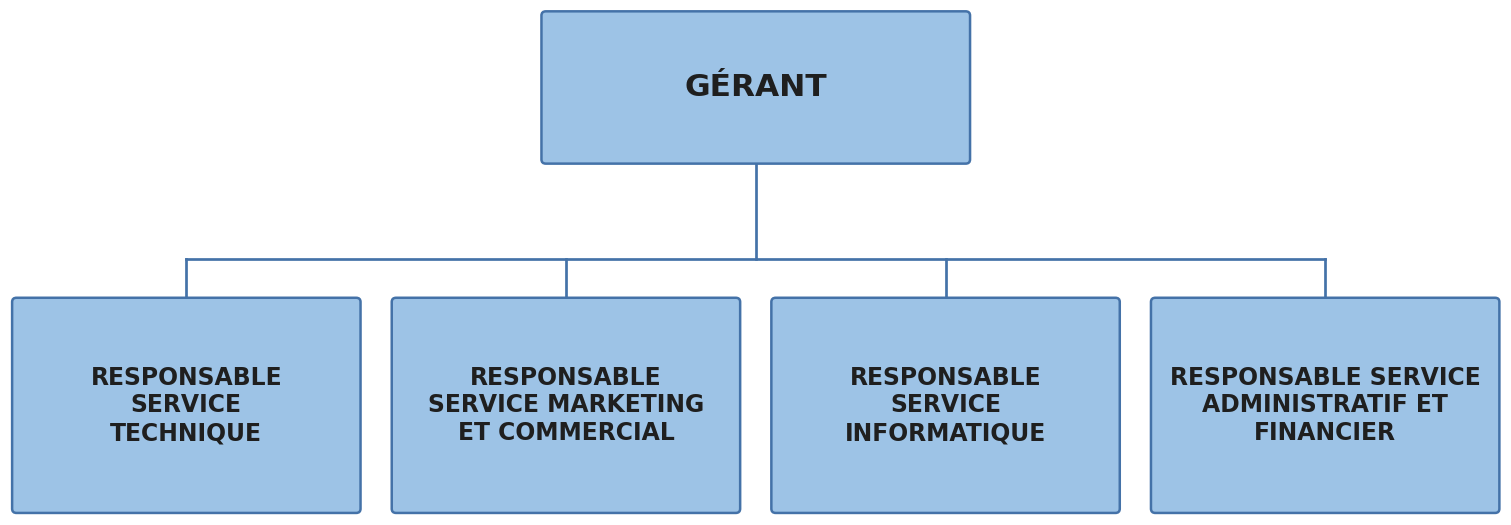
\includegraphics[width=0.9\textwidth]{capt1.png}
    \caption{Organigramme prévisionnel de l'entreprise}
    \label{fig:organigramme}
  \tablesourcepromoteurs

\end{figure}

\subsection{Définition des fonctions et attributions}

Dans toute organisation, chaque poste occupe une place précise et joue un rôle décisif dans le bon fonctionnement de l'ensemble. Les fonctions et attributions permettent de définir clairement les missions confiées à chaque responsable, afin d'assurer une meilleure répartition du travail, une bonne coordination des activités et une meilleure efficacité. La définition des fonctions vise à préciser les tâches, les responsabilités et les domaines d'intervention de chaque acteur de l'entreprise. Les attributions, quant à elles, déterminent les pouvoirs et les actions que chaque responsable est habilité à exercer dans le cadre de ses missions. Cette action d'organisation permet d'éviter les conflits de compétence, de faciliter la communication interne et de garantir l'atteinte des objectifs fixés par l'entreprise. Dans le cadre de ce projet, l'entreprise s'articule autour des postes suivants :
\begin{itemize}
        
    \item \textbf{Le Gérant}
    Il coiffe l'ensemble des autres services de l'entreprise; occupe une place centrale dans la structure organisationnelle et assure la coordination globale des activités en dirigeant, coordonnant, contrôlant et orientant toutes les activités vers la réalisation des objectifs fixés. Veille au fonctionnement intégral de chaque service en s'assurant que toutes les tâches sont correctement exécutées et en conformité avec les objectifs fixés par l'organisation. Le Gérant coordonne, organise et supervise les différentes actions menées au sein de l'entreprise afin d'assurer une bonne cohérence entre les services. En effet, il analyse les résultats obtenus, corrige les éventuels dysfonctionnements et met en place des stratégies pour améliorer la performance globale de l'entreprise. De plus, il sert de lien entre les différents services, favorisant ainsi une meilleure communication interne et une meilleure coordination du travail.

    \item \textbf{Responsable Service Technique}
    Le responsable du service technique constitue le cœur opérationnel du projet. Il est chargé de superviser et de coordonner l'ensemble des activités techniques de l'entreprise. Il veille au bon fonctionnement des équipements et des installations, organise les interventions de maintenance et s'assure de la qualité des travaux réalisés. Il garantit également le respect des normes de sécurité et propose des solutions techniques pour améliorer la performance et l'efficacité des services.

    \item \textbf{Responsable Service Marketing et Commercial}
    Le responsable du service marketing et commercial est un professionnel chargé à la fois de l'analyse du marché, de la définition des stratégies marketing et du développement des ventes de l'entreprise. Il étudie les besoins des consommateurs et la concurrence afin de proposer des actions adaptées pour promouvoir les produits ou services.
    Il met en place des campagnes de communication et des stratégies commerciales visant à attirer de nouveaux clients et à fidéliser la clientèle existante. Il participe également à la fixation des objectifs de vente, à la négociation avec les clients et au suivi des performances commerciales.
    En outre, il veille à la bonne image de l'entreprise, à la satisfaction des clients et à l'amélioration continue du chiffre d'affaires. Ainsi, il occupe un rôle essentiel dans la croissance et la compétitivité de l'organisation.

    \item \textbf{Responsable Service Informatique}
    Le responsable du service informatique est chargé du développement, du déploiement et de la maintenance de la plateforme logicielle d'Argos (application web d'administration, application mobile, API). Il s'occupe de l'administration des systèmes, des bases de données et de l'infrastructure cloud, ainsi que de la sécurité informatique et de la protection des données collectées. Il veille également à l'intégration des dispositifs embarqués avec la plateforme, au bon fonctionnement des serveurs et au support technique informatique auprès des autres services.

    \item \textbf{Responsable Service Administratif et Financier}
    Le responsable du service administratif et financier est chargé de la gestion des ressources financières de l'entreprise. Il veille à la bonne utilisation des fonds, à l'équilibre des dépenses et des recettes, ainsi qu'à la rentabilité des activités. Il élabore et suit le budget, contrôle les opérations comptables et financières, et s'assure du respect des obligations financières et fiscales. Il analyse également la situation financière de l'entreprise afin de proposer des solutions pour optimiser la gestion et soutenir la prise de décision. Sur le plan administratif, il assure également la gestion du personnel et des dossiers administratifs, le suivi des contrats et le respect des obligations légales et réglementaires de l'entreprise.


\end{itemize}
\subsection{Étude des ressources humaines}

Les ressources humaines jouent un rôle important dans le fonctionnement et la performance d'une entreprise. Elles permettent de valoriser le capital humain en assurant une bonne gestion du personnel, depuis le recrutement jusqu'à l'exploitation optimale des compétences de ce dernier. Elles contribuent à affecter les bonnes personnes aux bons postes, ce qui améliore l'efficacité et la productivité de l'organisation.

\subsubsection{Analyse des profils de poste}

Dans le but d'appréhender efficacement la répartition des rôles au sein de l'entreprise, il est nécessaire de procéder à une analyse des profils de poste. Cette démarche met en évidence les exigences propres à chaque fonction, tant en termes de compétences que de responsabilités.


\begin{table}[htbp]
    \centering
    \caption{Compétences relatives à chaque poste de responsabilité}
    \label{tab:competences}
    \renewcommand{\arraystretch}{1.5}
    \begin{tabularx}{\textwidth}{|>{\raggedright\arraybackslash}p{3cm}|X|X|}
        \hline
        \textbf{Postes de responsabilité} & \textbf{Buts recherchés} & \textbf{Compétences clés attendues} \\
        \hline
        \textbf{Gérant} & Veille au bon fonctionnement de chaque service de l'entreprise; oriente toutes les activités vers l'atteinte des objectifs de l'entreprise; s'assure de l'exécution correcte des tâches selon chaque service. & Sens du leadership, une vision globale et stratégique; capacité de prise de décision stratégique rapide et efficace; esprit d'analyse et de synthèse. \\
        \hline
        \textbf{Responsable Service Technique} & Organiser et coordonner les équipes techniques; assurer le bon fonctionnement des équipements et des installations (veiller à la maintenance préventive et corrective du matériel); contrôler la qualité des travaux techniques réalisés et s'assurer du respect des normes de sécurité et des procédures techniques; planifier les interventions techniques et les travaux à effectuer; proposer des solutions techniques pour améliorer les performances. & Sens de l'organisation et de la planification des activités et des équipes; maîtrise de la technologie; réactivité rapide face aux pannes; maîtrise des normes de sécurité; capacité d'adaptation et de résolution des problèmes complexes. \\
        \hline
        \textbf{Responsable Service Marketing et Commercial} & Augmenter le chiffre d'affaires de l'entreprise; attirer en mettant en exergue les campagnes de communication publicitaire; satisfaire et fidéliser la clientèle; proposer des actions pour améliorer le résultat de vente; étudier le marché et la concurrence pour mieux orienter les décisions stratégiques de l'entreprise. & Excellente aptitude en communication et en maîtrise de la gestion marketing; sens de l'organisation; connaissance suffisante de la concurrence et du marché; esprit de créativité; compétence avérée dans la conception et la mise en place de stratégie marketing efficace. \\
        \hline
        \textbf{Responsable du service informatique} & Développer et maintenir la plateforme logicielle d'Argos (application web, application mobile, API); administrer les serveurs, bases de données et l'infrastructure cloud; assurer la sécurité informatique et la protection des données collectées; intégrer les dispositifs embarqués à la plateforme et assurer le support technique informatique auprès des autres services. & Maîtrise du développement logiciel et des bases de données; connaissance des architectures cloud et des API; sens de la sécurité informatique; capacité à diagnostiquer et résoudre rapidement les incidents techniques; compétence en intégration de systèmes embarqués et de plateformes web/mobile. \\
        \hline
        \textbf{Responsable du service Administratif et Financier} & Gérer les ressources financières de l'entreprise et en optimiser la rentabilité ; élaborer et suivre le budget annuel ; garantir le respect des obligations fiscales, comptables et réglementaires ; assurer la gestion administrative du personnel. & Maîtrise de la comptabilité, de la finance d'entreprise et de la fiscalité ; grande rigueur, intégrité et esprit de synthèse ; connaissance du droit du travail et des affaires ; maîtrise des logiciels de gestion (ERP) ; capacité d'anticipation et d'analyse financière. \\
        \hline
    \end{tabularx}
  \tablesourcepromoteurs
\end{table}

\noindent cette répartition des responsabilités met en évidence une structure organisationnelle à la fois resserrée et hautement qualifiée, garantissant une couverture complète de la chaîne de valeur du projet ARGOS. De la direction générale, qui impulse la vision stratégique, aux pôles opérationnels spécialisés dans la technique, le commercial et l'informatique, chaque poste est adossé à des compétences clés rigoureusement adaptées aux exigences technologiques et logistiques du marché. Cette synergie des expertises assure une maîtrise globale du projet, allant de l'innovation IoT embarquée jusqu'à la commercialisation de la solution ARGOS.

\subsubsection{Équipe managériale}

Une équipe managériale désigne l'ensemble des personnes chargées de diriger, organiser et piloter les activités d'une organisation. Autrement dit, dans le cadre de notre projet, ce sont les principaux responsables des différents postes de responsabilité. Cette équipe se doit de posséder des compétences clés pour assurer pleinement son poste de responsabilité.

\begin{figure}[htbp]
    \centering
    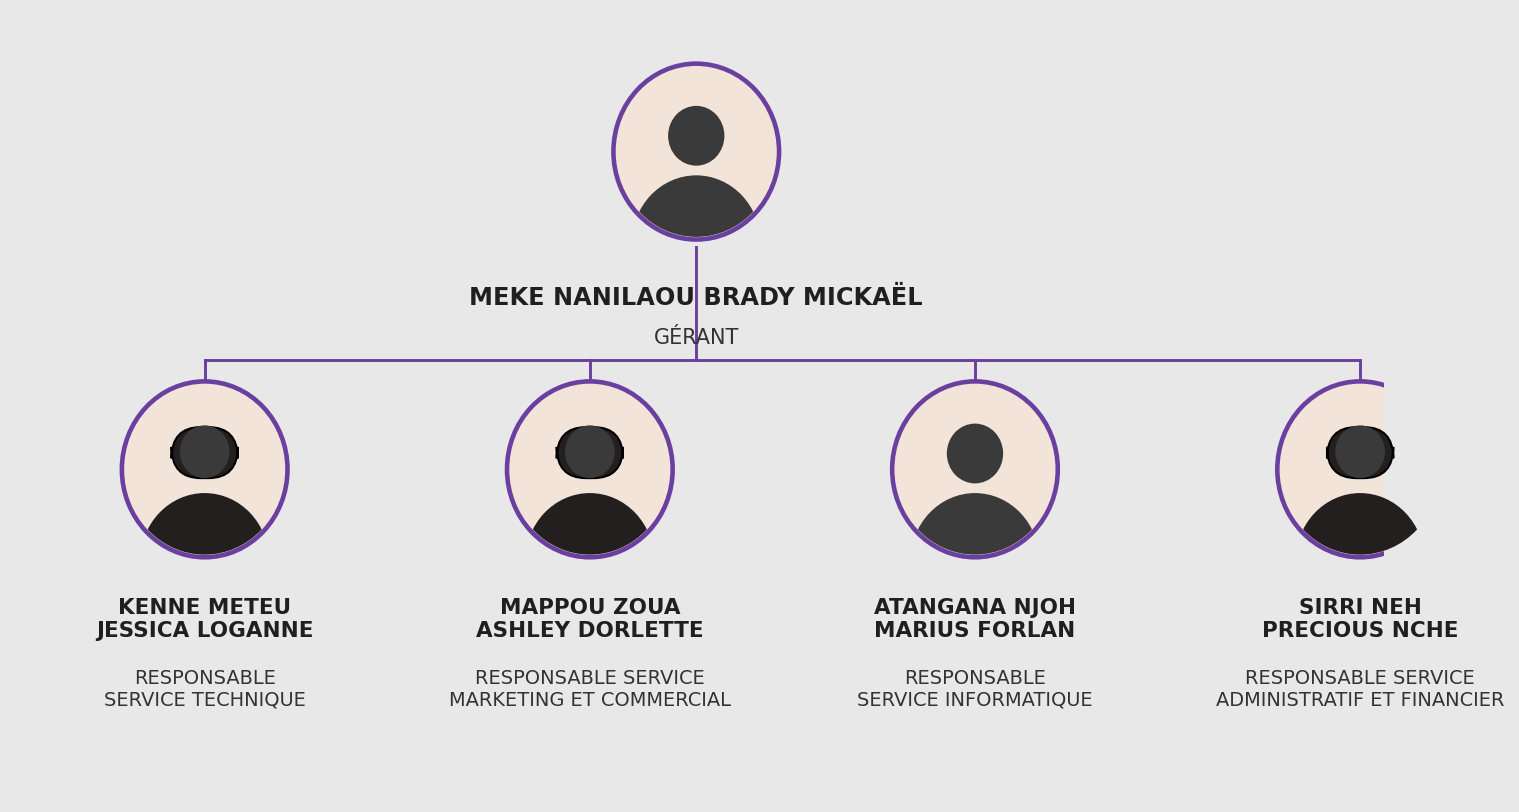
\includegraphics[width=0.9\textwidth]{capt2.png}
    \caption{Équipe managériale}
    \label{fig:equipe_manageriale}
    \tablesourcepromoteurs

\end{figure}

Le tableau ci-après présente une synthèse structurée des membres de l'équipe managériale, en mettant en lumière leurs fonctions respectives ainsi que leurs qualifications.

\begin{table}[htbp]
    \centering
    \caption{Composition de l'équipe managériale}
    \label{tab:composition_equipe}
    \renewcommand{\arraystretch}{1.5}
    \begin{tabularx}{\textwidth}{|>{\raggedright\arraybackslash}p{4cm}|>{\raggedright\arraybackslash}p{4.5cm}|X|}
        \hline
        \textbf{Postes de responsabilité} & \textbf{Responsables} & \textbf{Qualifications} \\
        \hline
        Gérant & MEKE NANILAOU BRADY MIKAEL & Ingénieur des travaux de télécommunications option Informatique et Réseau \\
        \hline
        Responsable Service Technique & KENNE METEU JESSICA LOGANNE & Ingénieur des travaux de télécommunications option Radiocommunication \\
        \hline
        Responsable Service Marketing et Commercial & MAPPOU ZOUA ASHLEY DORLETTE & Inspecteur des postes et télécommunications option Management des Télécommunications \\
        \hline
        Responsable du service informatique & ATANGANA NJOH MARIUS FORLAN & Ingénieur des travaux de télécommunications option Réseau et Télécommunications \\
        \hline
        Responsable Service Administratif et Financier & SIRRI NEH PRECIOUS NCHE & Inspecteur des postes et télécommunications option Comptabilité et Finance \\
        \hline
    \end{tabularx}
    \tablesourcepromoteurs

\end{table}

\subsubsection{Personnels à recruter}

Pour assurer le bon fonctionnement et le développement de notre système de boîte noire dédié aux conteneurs maritimes, nous allons procéder au recrutement de personnels qualifiés dont les profils, qualifications et compétences requises sont détaillés dans le tableau ci-dessous.

\begin{xltabular}{\textwidth}{|>{\raggedright\arraybackslash}p{3.4cm}|>{\centering\arraybackslash}p{0.8cm}|>{\raggedright\arraybackslash}p{3.1cm}|X|}
    \caption{Personnels à recruter} \label{tab:personnels_recruter} \\
    \hline
    \tableheadrow\thc{Poste} & \thc{Nb.} & \thc{Qualification} & \thc{Compétences} \\
    \hline
    \endfirsthead

    \multicolumn{4}{c}{\tablename~\thetable{} -- Personnels à recruter} \\
    \hline
    \tableheadrow\thc{Poste} & \thc{Nb.} & \thc{Qualification} & \thc{Compétences} \\
    \hline
    \endhead

    \endfoot
    
    \hline
    \endlastfoot

    Ingénieur en systèmes embarqués & 1 & BAC+5 en génie électronique & 
    \begin{itemize}[leftmargin=*, nosep, before=\vspace{-0.5\baselineskip}, after=\vspace{-0.5\baselineskip}]
        \item Conception et développement de systèmes d'acquisition de données embarqués
        \item Maîtrise des protocoles de communication (GPS, GPRS, satellite)
        \item Connaissance des normes maritimes (IMO, SOLAS)
        \item Intégration des capteurs (température, humidité, chocs, géolocalisation)
        \item Tests et validation des systèmes embarqués
    \end{itemize} \\
    \hline
    Ingénieur en développement logiciel & 1 & BAC+5 en informatique / Data Engineering & 
    \begin{itemize}[leftmargin=*, nosep, before=\vspace{-0.5\baselineskip}, after=\vspace{-0.5\baselineskip}]
        \item Développement d'applications de traitement et d'analyse de données
        \item Maîtrise des bases de données temps réel et des architectures cloud
        \item Développement d'interfaces de suivi et de visualisation cartographique
        \item Sécurisation des données et mise en œuvre de la cryptographie
        \item Connaissance des API de géolocalisation et de cartographie
    \end{itemize} \\
    \hline
    Responsable Technique et Qualité & 1 & BAC+3 en génie industriel / qualité & 
    \begin{itemize}[leftmargin=*, nosep, before=\vspace{-0.5\baselineskip}, after=\vspace{-0.5\baselineskip}]
        \item Assurer la conformité aux normes maritimes internationales (ISO, CE)
        \item Gestion des tests de résistance, d'étanchéité et certification (IP68, ATEX)
        \item Suivi et gestion des audits qualité et de la documentation technique
        \item Pilotage de la maintenance préventive et corrective des équipements
        \item Rédaction et mise à jour des rapports techniques et procédures qualité
    \end{itemize} \\
    \hline
    Responsable Commercial et Marketing & 1 & BAC+3 en commerce international & 
    \begin{itemize}[leftmargin=*, nosep, before=\vspace{-0.5\baselineskip}, after=\vspace{-0.5\baselineskip}]
        \item Développement et fidélisation du portefeuille clients dans le secteur
        \item Maîtrise des techniques de négociation et de vente B2B
        \item Connaissance approfondie du marché du transport maritime mondial
        \item Négociation des contrats avec les armateurs, transitaires et opérateurs
        \item Veille concurrentielle et analyse du marché
    \end{itemize} \\
    \hline
    Techniciens d'installation et de maintenance & 2 & BAC+2 en électronique / maintenance industrielle & 
    \begin{itemize}[leftmargin=*, nosep, before=\vspace{-0.5\baselineskip}, after=\vspace{-0.5\baselineskip}]
        \item Installation et configuration des boîtes noires sur les conteneurs
        \item Maintenance préventive et corrective des équipements électroniques
        \item Diagnostic et résolution des pannes matérielles et logicielles
        \item Formation et assistance technique des utilisateurs finaux
        \item Rédaction des rapports d'intervention et de suivi de maintenance
    \end{itemize} \\
    \hline
    Responsable Administratif et Juridique & 1 & BAC+3/5 en droit des affaires / administration & 
    \begin{itemize}[leftmargin=*, nosep, before=\vspace{-0.5\baselineskip}, after=\vspace{-0.5\baselineskip}]
        \item Assurer une veille juridique et réglementaire liée au secteur maritime
        \item Rédaction et suivi des contrats commerciaux, accords et conventions
        \item Gestion des contentieux et représentation de l'entreprise (justice)
        \item Capacité à planifier et organiser les tâches administratives
        \item Assurer le respect des obligations légales, fiscales et réglementaires
        \item Compétence dans la gestion de projets administratifs et institutionnels
    \end{itemize} \\
    \hline
    Secrétaire & 1 & BAC+2 en secrétariat / bureautique & 
    \begin{itemize}[leftmargin=*, nosep, before=\vspace{-0.5\baselineskip}, after=\vspace{-0.5\baselineskip}]
        \item Maîtrise des outils bureautiques (Word, Excel, PowerPoint)
        \item Rédaction et mise en forme de courriers, rapports et comptes-rendus
        \item Gestion du courrier entrant et sortant et archivage des documents
        \item Accueil physique et téléphonique des visiteurs et partenaires
        \item Organisation des réunions, agendas et déplacements professionnels
        \item Gestion administrative et suivi des dossiers du personnel
    \end{itemize} \\
    \hline
    Ménagère & 1 & BEPC / niveau primaire & 
    \begin{itemize}[leftmargin=*, nosep, before=\vspace{-0.5\baselineskip}, after=\vspace{-0.5\baselineskip}]
        \item Nettoyage et entretien quotidien des bureaux et espaces communs
        \item Lavage, repassage et entretien du linge de service
        \item Gestion et approvisionnement des produits d'entretien et ménagers
        \item Préparation et service des repas pour le personnel si nécessaire
        \item Maintien de l'hygiène et de la propreté de l'ensemble des locaux
        \item Gestion des déchets et respect des normes d'hygiène en vigueur
    \end{itemize} \\
    \hline
    Vigile & 1 & BEPC / formation en sécurité & 
    \begin{itemize}[leftmargin=*, nosep, before=\vspace{-0.5\baselineskip}, after=\vspace{-0.5\baselineskip}]
        \item Bonne condition physique et résistance à l'effort
        \item Surveillance et contrôle des accès aux locaux et installations
        \item Capacité à intervenir rapidement en cas d'incident ou d'intrusion
        \item Maîtrise des techniques de défense et de gestion des conflits
        \item Rédaction des rapports de ronde et d'incidents de sécurité
        \item Sens de la vigilance, rigueur et aptitude au travail de nuit
    \end{itemize} \\
\end{xltabular}
\noindent \textit{Source : Promoteurs 2025-2026}


\section{Étude de la faisabilité juridique et fiscale}

La présente étude vise à déterminer si et à quelles conditions le projet ARGOS est réalisable au regard des contraintes légales et fiscales applicables au Cameroun. Elle aboutit à des recommandations à mettre en œuvre, notamment en termes contractuel et fiscal, et constitue une étape primordiale afin de ne pas s'engager dans un projet qui pourrait se révéler illégal après avoir consenti des investissements importants.


\subsection{Faisabilité juridique}

Afin de préserver la force probante des données et de garantir la conformité réglementaire de la solution, plusieurs risques juridiques critiques doivent être anticipés dès la phase de conception a savoir :
\begin{itemize}
    \item \textbf{Preuve légale des données :} en cas de litige, la valeur probante des données dépend notamment de la capacité à démontrer leur intégrité, leur traçabilité et les conditions de leur conservation. Une évaluation technique indépendante du dispositif et de la chaîne de données peut renforcer cette démonstration, sans constituer à elle seule une garantie automatique d'admission de la preuve.
    \item \textbf{Conformité maritime :} l'emploi du dispositif doit être examiné au regard des règles applicables au conteneur et à la cargaison, notamment la convention SOLAS et, en présence de marchandises dangereuses, le code IMDG\cite{imo_solas,imo_imdg}. L'OMI édicte ces instruments internationaux, mais n'homologue pas directement chaque boîtier commercialisé. Les essais, homologations et certificats requis doivent être obtenus auprès des autorités nationales compétentes et, selon le cas, d'organismes techniques reconnus.
    \item \textbf{Protection des données et RGPD :} le RGPD s'applique lorsque le traitement entre dans son champ territorial et porte sur des données relatives à une personne physique identifiée ou identifiable, notamment des données de localisation. Le simple transit d'un conteneur dans l'Union européenne ne suffit donc pas, à lui seul, à déclencher l'application du règlement\cite{rgpd_officiel}.
    \item \textbf{Télécommunications et importation :} les équipements de communications électroniques ou installations radioélectriques doivent faire l'objet des formalités d'homologation applicables auprès de l'Agence de Régulation des Télécommunications (ART). Le dossier comprend notamment les spécifications techniques, la déclaration de conformité du fabricant et les rapports d'essais\cite{art_homologation}. Le classement tarifaire et les droits de douane doivent être confirmés auprès de la Direction Générale des Douanes avant l'importation ; aucun taux forfaitaire de 40~\% n'est retenu ici faute de source officielle vérifiée.
\end{itemize}

La maîtrise de ces quatre enjeux juridiques des valeur probante des données, des conformité maritime internationale, des protection des données personnelles et régularité douanière et conditionne la solidité juridique du projet Argos et confirme sa faisabilité sur ce plan, sous réserve des démarches de certification et d'homologation évoquées.

\subsubsection{Statut juridique}

La forme de statut juridique (ou forme juridique) d'une entreprise désigne le cadre légal imposé à une activité économique. L'article 4 de l'Acte uniforme OHADA relatif au droit des sociétés commerciales et du groupement d'intérêt économique dispose :

« la société commerciale est créée par deux ou plusieurs personnes qui conviennent par contrat, d'affecter à une activité, des biens en numéraire ou en nature, dans le but de partager les bénéfices ou de profiter de l'économie qui pourra en résulter »\cite{ohada_auscgie}.

Les règles applicables régissant l'activité de l'entreprise sont donc tributaires de ce statut. Le choix du statut entraîne diverses conséquences notamment juridiques au sein d'une entreprise.

Dans le cadre de notre projet ARGOS, nous optons pour le statut de Société à Responsabilité Limitée (SARL) pour les raisons suivantes :

\begin{table}[htbp]
    \centering
    \caption{Justification du choix de la SARL}
    \label{tab:choix_sarl}
    \renewcommand{\arraystretch}{1.5}
    \begin{tabularx}{\textwidth}{|>{\raggedright\arraybackslash}p{4cm}|X|}
        \hline
        \textbf{Critère} & \textbf{Justification} \\
        \hline
        Limitation des risques & La responsibilite des associés est limitée à leurs apports, protégeant ainsi le patrimoine personnel des promoteurs. \\
        \hline
        Protection sociale & Affiliation à la CNPS des travailleurs salariés employés par la société, dans les conditions prévues par la réglementation sociale. \\
        \hline
        Accès au code des investissements & Possibilité de bénéficier des mesures incitatives prévues par la réglementation camerounaise. \\
        \hline
        Capital social & Capital fixé par les associés dans le respect des dispositions OHADA et nationales applicables. \\
        \hline
        Protection patrimoniale & Protection du patrimoine personnel en cas de faillite. \\
        \hline
        Crédibilité & Recherche d'une crédibilité auprès des investisseurs et partenaires institutionnels. \\
        \hline
    \end{tabularx}
    \tablesourcepromoteurs
\end{table}
La fiche d'identité de l'entreprise se présente comme suit :
\begin{table}[htbp]
    \centering
    \caption{Fiche d'identité de l'entreprise ARGOS}
    \label{tab:fiche_identite}
    \renewcommand{\arraystretch}{1.5}
    \begin{tabularx}{\textwidth}{|>{\raggedright\arraybackslash}p{4cm}|X|}
        \hline
        \textbf{Élément} & \textbf{Information} \\
        \hline
        Raison sociale & ARGOS SARL \\
        \hline
        Forme juridique & SARL \\
        \hline
        Capital & 20 000 000 FCFA \\
        \hline
        Activité & Conception, fabrication et commercialisation de solutions de traçabilité et de monitoring intelligent pour conteneurs maritimes \\
        \hline
        Secteur d'activité & Télécommunications, TIC, Électronique, IoT (Internet des Objets) \\
        \hline
        Produits & Dispositif embarqué « boîte noire » ARGOS + Plateforme de supervision logicielle \\
        \hline
        Siège social & Douala (zone portuaire stratégique) \\
        \hline
        Téléphone & 220 10 29 07 \\
        \hline
        E-mail & Argos@argos-sarl.com \\
        \hline
        Année de création & 2026 \\
        \hline
    \end{tabularx}
    \tablesourcepromoteurs
\end{table}

L’analyse comparative des statuts juridiques conduit à l'adoption de la Société à Responsabilité Limitée (SARL), dont les motivations stratégiques sont synthétisées dans le Tableau \ref{tab:choix_sarl}. Ce tableau met en lumière les avantages majeurs de cette forme juridique, notamment la limitation de la responsabilité des associés à leurs apports et protégeant ainsi leur patrimoine personnel, leur accès aux avantages du Code des investissements au Cameroun, ainsi qu'une crédibilité renforcée auprès des partenaires financiers et institutionnels.

Dans la continuité de ce choix organisationnel, la formalisation de l'entreprise se concrétise à travers sa carte d'identité officielle présentée dans le Tableau \ref{tab:fiche_identite}. Ce récapitulatif structure l'ensemble des informations clés d'ARGOS SARL et de sa raison sociale à son capital social fixé à 20\,000\,000 FCFA, en passant par son positionnement au cœur du pôle stratégique de Douala et ses domaines d'expertise en IoT et télécommunications. Ce tableau constitue ainsi la boussole institutionnelle de l'entreprise, garantissant sa lisibilité auprès des autorités réglementaires et des acteurs de la chaîne logistique.

\subsubsection{Régime d'imposition de l'entreprise}

Le régime d'imposition est un dispositif fiscal qui fixe l'ensemble des règles facilitant la détermination des impôts et des taxes. Conformément aux dispositions de l'article 93 du Code Général des Impôts (CGI), les contribuables relèvent des régimes ci-après, déterminés notamment en fonction du chiffre d'affaires réalisé\cite{cgi_cameroun}.

\begin{table}[htbp]
    \centering
    \caption{Régimes d'imposition au Cameroun}
    \label{tab:regimes_imposition}
    \renewcommand{\arraystretch}{1.5}
    \begin{tabularx}{\textwidth}{|>{\raggedright\arraybackslash}p{4cm}|>{\raggedright\arraybackslash}p{5cm}|X|}
        \hline
        \textbf{Régime} & \textbf{Conditions} & \textbf{Caractéristiques} \\
        \hline
        Régime de l'impôt libératoire & CA annuel HT $<$ 10 000 000 FCFA & Entreprises individuelles uniquement \\
        \hline
        Régime simplifié & CA annuel HT $\geq$ 10 000 000 FCFA et $<$ 50 000 000 FCFA & Entreprises individuelles et personnes morales \\
        \hline
        Régime du réel & CA annuel HT $\geq$ 50 000 000 FCFA & Entreprises individuelles et personnes morales \\
        \hline
    \end{tabularx}
    \tablesourcepromoteurs

\end{table}

\paragraph{Régime applicable à ARGOS :}
Au vu de notre chiffre d'affaires prévisionnel (186 685 000 FCFA la première année, 465 500 000 FCFA la deuxième année, 928 300 000 FCFA la troisième année), notre entreprise relèvera du régime réel dès la première année d'activité\cite{cgi_cameroun}.

\paragraph{L'impôt sur les sociétés (IS) applicable aux SARL :}
Les SARL entrent dans le champ de l'impôt sur les sociétés. Le CGI fixe le taux de droit commun à 30~\% et prévoit un taux de 25~\% pour les contribuables dont le chiffre d'affaires est inférieur ou égal à 3 milliards de FCFA, sous réserve des autres conditions et régimes particuliers prévus par les textes\cite{cgi_cameroun}.

\paragraph{Exonérations fiscales pour les nouvelles entreprises (Loi de Finances 2025) :}
La fiscalité camerounaise prévoit des mesures incitatives, mais celles-ci ne sont pas automatiques du seul fait de la création d'une société ou de son activité dans les TIC. Leur bénéfice dépend de l'éligibilité du projet, de l'obtention de l'agrément requis et du respect des obligations prévues par le régime applicable\cite{incitations2025}.

ARGOS devra donc vérifier son éligibilité avant d'inscrire un avantage fiscal dans ses prévisions. Les avantages susceptibles d'être sollicités peuvent porter sur :
\begin{itemize}
    \item les mesures prévues par le régime d'incitation à l'investissement auquel le projet serait agréé ;
    \item les facilités fiscales ou douanières expressément mentionnées dans la décision d'agrément ;
    \item les dispositifs sectoriels auxquels l'entreprise démontrerait son éligibilité.
\end{itemize}
\textbf{Attention :} Les exonérations sont conditionnées au respect des obligations déclaratives et comptables. En cas de non-respect, l'administration fiscale peut retirer l'avantage et appliquer l'IS rétroactivement.

\subsubsection{Obligations de l'entreprise}

Les obligations sociales de notre entreprise ARGOS sont nombreuses. Nous les présentons ci-après.
\begin{table}[htbp]
    \centering
    \caption{Obligations fiscales de l'entreprise}
    \label{tab:obligations_fiscales}
    \renewcommand{\arraystretch}{1.5}
    \begin{tabularx}{\textwidth}{|>{\raggedright\arraybackslash}p{4cm}|X|p{3cm}|}
        \hline
        \textbf{Obligation} & \textbf{Description} & \textbf{Échéance} \\
        \hline
        Numéro de contribuable & Acquisition obligatoire avant le début de l'activité & Immédiat \\
        \hline
        IRPP & Déclaration et paiement des retenues sur salaires & Mensuel \\
        \hline
        Immatriculation fiscale & Obtention de l'attestation d'immatriculation fiscale & À la création \\
        \hline
        Enregistrement du bail & 10~\% du montant global du loyer annuel si l'entreprise est locataire & À la signature \\
        \hline
        Précompte sur loyer & Retenue de 5~\% sur le loyer & Mensuel \\
        \hline
        Taxe sur la publicité & Plaques publicitaires site commerciale. & Annuel \\
        \hline
        TVA & Déclaration et paiement (taux : 19,25~\%) & Mensuel/Trimestriel \\
        \hline
        Patente & Déclaration et paiement, sauf exonération expressément applicable & Annuel \\
        \hline
        Acompte sur IS & 1,5~\% + CAC sur l'IS & Mensuel \\
        \hline
        IS de clôture & Complément d'impôt sur les sociétés en fin d'exercice & Annuel \\
        \hline
    \end{tabularx}
    \noindent\textit{Source : Promoteurs, à partir du Code général des impôts\cite{cgi_cameroun}.}
\end{table}

\noindent Le Tableau~\ref{tab:obligations_fiscales} dresse un panorama exhaustif du cadre fiscal régissant les activités d'ARGOS SARL au Cameroun. L'importance de ce tableau réside dans sa capacité à cartographier rigoureusement les différentes échéances (mensuelles, annuelles ou ponctuelles) et les taxes applicables (TVA, IRPP, acomptes sur IS). Cette visibilité fiscale est indispensable pour l'entreprise afin d'anticiper sa trésorerie, de planifier ses charges d'exploitation et de garantir une conformité totale avec l'administration fiscale, sécurisant ainsi la pérennité financière de la structure.

\bigskip

\begin{table}[htbp]
    \centering
    \caption{Obligations sociales de l'entreprise}
    \label{tab:obligations_sociales}
    \renewcommand{\arraystretch}{1.5}
    \begin{tabularx}{\textwidth}{|>{\raggedright\arraybackslash}p{4cm}|X|}
        \hline
        \textbf{Obligation} & \textbf{Description} \\
        \hline
        Immatriculation du personnel & Déclaration à la CNPS de tout personnel employé \\
        \hline
        Cotisations CNPS & Déclaration et paiement des retenues sur salaire (allocations familiales, pension vieillesse, accidents de travail) \\
        \hline
        DIPE & Tenue du Document d'Information sur le Personnel Employé \\
        \hline
        Registres obligatoires & Tenue du livret de paie, du registre du personnel, du règlement intérieur, des fascicules 1, 2 et 3 du personnel employé \\
        \hline
    \end{tabularx}
    \noindent\textit{Source : CNPS et Code général des impôts\cite{cnps_employeurs,cgi_cameroun}.}
\end{table}

\noindent le Tableau~\ref{tab:obligations_sociales} synthétise les exigences réglementaires en matière de gestion des ressources humaines et de protection sociale. Ce récapitulatif met en lumière l'engagement de l'entreprise envers ses collaborateurs à travers l'immatriculation auprès de la CNPS, la gestion rigoureuse des cotisations et la tenue des documents obligatoires (DIPE, registres de paie). L'importance de ce dispositif réside dans le respect des droits des salariés, la prévention des risques de contentieux avec les institutions de contrôle du travail et la construction d'un climat social stable et professionnel au sein d'ARGOS SARL.

\paragraph{Obligations liées à la protection des données personnelles (Loi n°2024/017) :}
La loi n°2024/017 du 23 décembre 2024 encadre au Cameroun la collecte et les autres opérations de traitement portant sur des données à caractère personnel. Les traitements mis en œuvre par ARGOS doivent être examinés et mis en conformité avec ce texte\cite{loi2024_donnees}.
Notre plateforme ARGOS étant amenée à traiter des données de géolocalisation et des informations sensibles sur les marchandises et les conteneurs, nous devons Obtenir le consentement explicite des utilisateurs pour la collecte et le traitement des données , Assurer la transparence sur les finalités du traitement , Garantir les droits des personnes (accès, rectification, effacement, opposition, portabilité) ,Notifier toute violation de données à l'autorité compétente ,Encadrer les transferts internationaux de données.

\textbf{Sanctions :} le non-respect de la loi expose le responsable du traitement aux sanctions administratives et pénales prévues par ce texte\cite{loi2024_donnees}.

\subsubsection{Processus de création de l'entreprise}

La formalisation d'une société s'effectue auprès du Centre de Formalités de Création d'Entreprises (CFCE), qui centralise les principales démarches de création. Le dossier d'une société commerciale comprend notamment les statuts, la déclaration requise pour la SARL, la liste des dirigeants ou associés et un plan de localisation\cite{minpmeesa_cfce}.

\paragraph{Phase 1 : Création de l'entreprise au CFCE }

\indent Pour une SARL, la procédure comprend notamment les opérations suivantes :
\begin{itemize}
    \item établissement des statuts dans la forme requise et préparation des déclarations de constitution ;
    \item dépôt du dossier au CFCE pour l'immatriculation au RCCM, l'immatriculation fiscale et les formalités sociales applicables.
\end{itemize}

\paragraph{Phase 2 : Enregistrement de l'entreprise}

\indent Les documents nécessaires pour l'enregistrement auprès du centre des impôts sont :
\begin{itemize}
    \item Le Registre du commerce ;
    \item Les statuts ;
    \item L'attestation d'immatriculation ;
    \item Le plan de localisation ;
    \item Le contrat de bail.
\end{itemize}

\subsubsection{Bilan du coût total de création d'entreprise}

La création légale de la société ARGOS SARL implique un ensemble de démarches administratives, notariales et fiscales. Afin de budgétiser précisément la phase de lancement, le tableau ci-dessous récapitule l'intégralité des frais liés à l'immatriculation et à l'obtention des documents officiels. Ce bilan financier constitue le coût d'entrée indispensable pour formaliser l'existence juridique de l'entreprise.

\begin{table}[H]
    \centering
    \caption{Coût de création de l'entreprise}
    \label{tab:cout_creation}
    \renewcommand{\arraystretch}{1.5}
    \begin{tabularx}{\textwidth}{|>{\raggedright\arraybackslash}p{3.5cm}|>{\raggedright\arraybackslash}p{4cm}|c|X|}
        \hline
        \textbf{Organe concerné} & \textbf{Pièces à obtenir} & \textbf{Montant (FCFA)} & \textbf{Observation} \\
        \hline
        Greffe du tribunal de 1ère instance & Extrait du casier judiciaire & 12 500 & 2 500 FCFA $\times$ 5 associés \\
        \hline
        CNPS & Attestation de soumission CNPS & 8 000 & 6 000 FCFA + 2 timbres de 1 000 FCFA \\
        \hline
        CNPS & Attestation de non-utilisation du personnel salarié & 2 500 & \\
        \hline
        Centre des impôts & Carte de contribuable & Exonéré & Exonération pendant les 5 premières années \\
        \hline
        Centre des impôts & Attestation d'exonération à la patente & Exonéré & Exonération pendant les 5 premières années \\
        \hline
        RCCM & Attestation d'immatriculation & 41 500 minimum & Montant minimal publié par le MINPMEESA ; coût variable selon le dossier \\
        \hline
        Notaire & Frais notariés & 80 000 & Mise en place de la SARL \\
        \hline
        \textbf{Total estimatif} & \multicolumn{3}{l|}{\textbf{144 500 FCFA minimum, à confirmer par devis et quittances}} \\
        \hline
    \end{tabularx}
    \noindent\textit{Source : estimations des promoteurs ; montant minimal du RCCM vérifié auprès du MINPMEESA\cite{minpmeesa_cfce}.}
\end{table}

\subsubsection{Bilan des risques et opportunités}

Le déploiement d'une solution technologique innovante dans le secteur maritime expose naturellement l'entreprise à divers aléas. Pour garantir la viabilité du projet ARGOS, il est crucial de cartographier ces menaces potentielles. Le tableau suivant identifie et catégorise les principaux risques juridiques, fiscaux et sectoriels susceptibles d'impacter nos opérations.

\begin{table}[H]
    \centering
    \caption{Identification des risques}
    \label{tab:identification_risques}
    \renewcommand{\arraystretch}{1.5}
    \begin{tabularx}{\textwidth}{|>{\raggedright\arraybackslash}p{4cm}|X|}
        \hline
        \textbf{Catégorie} & \textbf{Description des risques} \\
        \hline
        Risques juridiques & Non-conformité à la loi 2024/017 sur la protection des données personnelles; Contentieux liés à la responsabilité des données de localisation; Évolution des réglementations maritimes (OMI). \\
        \hline
        Risques fiscaux & Perte des avantages fiscaux en cas de non-respect des obligations déclaratives; Requalification fiscale du régime d'imposition; Changement de la législation fiscale. \\
        \hline
        Risques sectoriels & Concurrence des multinationales; Évolution rapide des technologies; Dépendance aux fournisseurs de composants électroniques. \\
        \hline
    \end{tabularx}
    \tablesourcepromoteurs
\end{table}

L'identification de ces vulnérabilités n'est qu'une première étape ; elle doit impérativement s'accompagner de mesures préventives et correctives. Ainsi, le tableau ci-après détaille la stratégie de gestion des risques adoptée par ARGOS pour atténuer ces menaces, sécuriser l'investissement et transformer ces défis en avantages concurrentiels.

\begin{table}[H]
    \centering
    \caption{Plan d'action contre les risques}
    \label{tab:plan_action_risques}
    \renewcommand{\arraystretch}{1.5}
    \begin{tabularx}{\textwidth}{|>{\raggedright\arraybackslash}p{4cm}|X|}
        \hline
        \textbf{Risque} & \textbf{Plan d'action} \\
        \hline
        Risques juridiques & Désigner un Délégué à la Protection des Données (DPO); Mettre en conformité la plateforme avant le 23 juin 2026; Rédiger des conditions générales d'utilisation et une politique de confidentialité claires. \\
        \hline
        Risques fiscaux & Se faire accompagner par un expert-comptable; Respecter scrupuleusement les délais de déclaration; Conserver toutes les preuves d'éligibilité aux exonérations. \\
        \hline
        Risques sectoriels & Placer l'innovation au cœur de la stratégie; Diversifier les fournisseurs; Surveiller l'évolution de la concurrence et du marché. \\
        \hline
    \end{tabularx}
    \tablesourcepromoteurs
\end{table}


\subsection{Étude de la faisabilité fiscale}

Sur le plan fiscal, plusieurs démarches conditionnent la viabilité du projet ARGOS et doivent être anticipées afin d'éviter tout blocage administratif ou surcoût imprévu, lesquelles s'articulent autour des points suivants :
\begin{itemize}
    \item \textbf{Agrément aux incitations à l'investissement :} ARGOS peut déposer une demande auprès du guichet compétent prévu par le régime des incitations à l'investissement. La nature et la durée des avantages ne doivent être intégrées au plan financier qu'après vérification de l'éligibilité et délivrance d'un agrément précisant les facilités accordées\cite{incitations2025}.
    \item \textbf{Classement tarifaire douanier :} il est nécessaire de démontrer auprès de la Direction Générale des Douanes (DGD) que le boîtier Argos ne relève pas de la catégorie générique des « appareils électroniques », dont le taux de taxation est plus élevé, mais d'une catégorie plus adaptée à sa fonction de dispositif de traçabilité logistique, afin d'obtenir un classement tarifaire plus favorable.
    \item \textbf{Autorisations techniques et coordination portuaire :} une coordination avec le Port Autonome de Douala peut faciliter l'expérimentation en zone portuaire, mais elle ne supprime pas automatiquement les taxes ou redevances applicables. L'homologation d'un équipement de communications électroniques ou radioélectrique relève de la procédure publiée par l'ART\cite{art_homologation}.
\end{itemize}

La sécurisation de ces trois démarches fiscales et douanières conditionne la rentabilité du modèle économique d'Argos et confirme la faisabilité fiscale du projet, sous réserve de leur mise en œuvre effective.


\subsubsection{Synthèse}

L'étude de faisabilité juridique et fiscale du projet ARGOS démontre que la création d'une SARL est juridiquement viable et fiscalement avantageuse dans le contexte camerounais actuel.

\begin{table}[htbp]
    \centering
    \caption{Synthèse de l'étude juridique et fiscale}
    \label{tab:synthese_etude}
    \renewcommand{\arraystretch}{1.5}
    \begin{tabularx}{\textwidth}{|>{\raggedright\arraybackslash}p{4cm}|X|}
        \hline
        \textbf{Aspect} & \textbf{Constat} \\
        \hline
        Statut juridique & SARL adaptée pour limiter les risques et bénéficier d'une crédibilité auprès des investisseurs. \\
        \hline
        Régime fiscal & Régime réel dès la première année au regard du chiffre d'affaires prévisionnel ; avantages fiscaux uniquement sous réserve d'éligibilité et d'agrément. \\
        \hline
        Protection des données & Obligation de conformité des traitements à la loi n°2024/017. \\
        \hline
        Coût de création & Environ 124 500 FCFA (hors capital social). \\
        \hline
        Capital social & 20 000 000 FCFA (apports des 5 associés fondateurs). \\
        \hline
    \end{tabularx}
    \tablesourcepromoteurs
\end{table}

 ce chapitre a permis de démontrer la faisabilité globale du projet ARGOS en validant successivement ses dimensions technique, organisationnelle, juridique et fiscale. Sur le plan technique, les solutions apportées pour surmonter les défis critiques — tels que l'autonomie énergétique en haute mer, la connectivité en zone blanche, la sécurité physique du boîtier et la cybersécurité des données confirment la robustesse de l'architecture retenue. L'analyse organisationnelle a mis en évidence une structure managériale solide (SARL) portée par une équipe aux compétences complémentaires, soutenue par un plan de recrutement ciblé pour accompagner la croissance de l'entreprise. Enfin, l'étude juridique et fiscale a validé le choix de la Société à Responsabilité Limitée (SARL), garantissant une protection patrimoniale adéquate, une conformité stricte aux réglementations en vigueur (notamment la loi n°2024/017 sur la protection des données) et un accès stratégique aux mesures incitatives du code des investissements camerounais. Ces fondations étant posées et sécurisées, il convient à présent d'évaluer la rentabilité et la robustesse économique de ce modèle à travers l'étude de viabilité financière, objet du chapitre suivant.

	% --- Définition des couleurs institutionnelles (Bleu Nuit & Bleu Clair) ---
% Couleurs historiques des tableaux du chapitre 4.
\colorlet{BleuNuit}{argostablehead}
\colorlet{BleuClair}{argostablerow}
% La couleur des filets est gérée globalement par le préambule.
% Certaines lignes historiques appliquent \rowcolor dans chaque cellule.
% \cellcolor conserve le rendu attendu sans provoquer d'erreur d'alignement.
\renewcommand{\rowcolor}[1]{\cellcolor{#1}}

\chapter{Étude de la viabilité}
\label{chap:viabilite_financière}

L’étude de la viabilité financière permet d’évaluer la rentabilité prévisionnelle pour notre projet ARGOS a généré une technique de gestion qui a pour objectif de donner une vision synthétique de la situation financière d’un projet. Elle consiste également à valoriser les flux financiers résultant des études précédentes afin de déterminer la rentabilité d’un projet, tout ceci sur la base des prévisions financières qui seront ressorties. Cette étude constitue un outil d’aide à la décision stratégique. Elle s’adresse aux porteurs de projet, aux partenaires financiers et aux investisseurs désireux de s’assurer de la solidité économique du projet. Pour y parvenir, nous allons élaborer les différents états financiers prévisionnels ensuite présenter quelques indicateurs de la rentabilité du projet.

\section{Prévisions financières}
L’établissement de nos prévisions financières s’appuie sur les différentes hypothèses issues de l’étude de marché et de l’analyse stratégique menées dans les chapitres précédents. Cette partie nous permet d’évaluer le coût total de notre projet et de ressortir l’origine des ressources financières. Pour réaliser notre projet, nous aurons besoin de matériels informatiques, logiciels et matériels de bureau qui favoriseront le démarrage de notre activité. Nous allons aussi évaluer le montant de la charge salariale qui nous aidera à estimer notre besoin en fonds de roulement initial (BFR).

% \\\\\\\\\\\\\\\\\\\\\\\\\\\\\\\\\\\\\\\\\\\\\\\\\\\\\\\\\\\\\  analyse previsionnels


\subsection{Analyse fréquentielle des flux de conteneurs en Afrique centrale}

La rentabilité du modèle économique ARGOS repose sur un nombre suffisant de trajets de conteneurs pour générer les revenus nécessaires à couvrir les coûts d’investissement et d’exploitation. Cette section présente une analyse approfondie des données réelles des principaux ports d’Afrique centrale.
% \\\\\\\\\\\\\\\\\\\\\\\\\  ajouter d'ici 

\subsubsection{Port de Douala (Cameroun) : Pôle historique}
Le Port Autonome de Douala (PAD) constitue le hub maritime le plus important d’Afrique centrale, concentrant entre 71\,\% et 76\,\% du volume global de trafic maritime camerounais selon l’analyse sectorielle du transport maritime camerounais publié le 1er février 2026\cite{pad2025}.

\begin{table}[ht]
\centering
\caption{Trafic du Port de Douala (2023-2024)} \label{tab:trafic_douala}
\begin{tabularx}{\textwidth}{@{}Xrrc@{}}
\toprule
\rowcolor{BleuNuit}\color{white}\textbf{Indicateur} & \rowcolor{BleuNuit}\color{white}\textbf{2023} & \rowcolor{BleuNuit}\color{white}\textbf{2024} & \rowcolor{BleuNuit}\color{white}\textbf{Évolution} \\
\midrule
Traffic export-import (tonnes) & 12 190 000 & 12 920 000 & +6,0\,\% \\
\rowcolor{BleuClair}Mouvements de navires & 1 450 & 1 520 & +4,8\,\% \\
Durée moyenne de service (jours) & 5,2 & 5,2 & — \\
\bottomrule
\end{tabularx}
\end{table}
\tablesourcepromoteurs

L'analyse de l'activité du Port Autonome de Douala met en évidence une dynamique de croissance soutenue de ses plateformes logistiques\cite{pad2025}. 
Entre 2023 et 2024, le trafic global des marchandises à l'exportation et à l'importation a progressé de 6\,\% 
pour atteindre 12,92 millions de tonnes (soit une augmentation notable de plus de 720\,000 tonnes sur une période d'un an)\cite{pad2025}. 
Cette vitalité opérationnelle s'accompagne d'une hausse du trafic maritime, matérialisée par 1\,520 mouvements de navires en 2024 (en augmentation de 4,8\,\% par rapport à l'exercice précédent), 
venant s'inscrire dans une trajectoire globale d'activité cumulée à plus de 5\,200 escales sur la période quinquennale récente\cite{pad2025}. 
Enfin, la durée moyenne de séjour et de service des unités (maintenue de manière constante à 5,2 jours) témoigne d'une stabilisation des opérations de traitement portuaire\cite{pad2025}, 
tout en soulignant la marge d'optimisation temporelle que des solutions de traçabilité avancée comme ARGOS peuvent 
contribuer à combler.

\subsubsection{Port de Kribi (Cameroun) : Croissance exponentielle}
Le Port Autonome de Kribi (PAK) connaît une dynamique de croissance exceptionnelle, avec un trafic conteneurisé multiplié par plus de quatre entre 2018 et 2025\cite{pak2026}. Cette affirmation est confirmée par les rapports officiels et les analyses sectorielles récents sur la performance portuaire du Cameroun, qui soulignent la progression spectaculaire du Port Autonome de Kribi (PAK) entre 2018 et 2025\cite{pak2026}.

\begin{xltabular}{\textwidth}{@{} X r r @{}}
\caption{Évolution du trafic conteneurs à Kribi (2018-2025)} \label{tab:trafic_kribi} \\
\toprule
\rowcolor{BleuNuit}\color{white}\textbf{Année} & \rowcolor{BleuNuit}\color{white}\textbf{Trafic conteneurs (EVP)} & \rowcolor{BleuNuit}\color{white}\textbf{Évolution annuelle} \\
\midrule
\endfirsthead
\multicolumn{3}{c}{\tablename\ \thetable{} -- Suite de la page précédente} \\
\toprule
\rowcolor{BleuNuit}\color{white}\textbf{Année} & \rowcolor{BleuNuit}\color{white}\textbf{Trafic conteneurs (EVP)} & \rowcolor{BleuNuit}\color{white}\textbf{Évolution annuelle} \\
\midrule
\endhead
\midrule
\multicolumn{3}{r}{\textit{Suite à la page suivante...}} \\
\endfoot
\bottomrule
\multicolumn{3}{l}{\textit{Source : Les Promoteurs 2025-2026}} \\
\endlastfoot
2018 & 135 820 & — \\
\rowcolor{BleuClair}2019 & 153 403 & +13,0\,\% \\
2020 & 239 871 & +56,4\,\% \\
\rowcolor{BleuClair}2021 & 210 042 & -12,4\,\% \\
2022 & 277 862 & +32,3\,\% \\
\rowcolor{BleuClair}2023 & 275 063 & -1,0\,\% \\
2024 & 304 546 & +10,7\,\% \\
2025 & 555 398 & +82,4\,\% \\
\end{xltabular}

L'analyse de l'évolution du trafic de conteneurs au Port Autonome de Kribi entre 2018 et 2025 révèle une trajectoire d'expansion remarquable, illustrant la montée en puissance de ce hub portuaire stratégique\cite{pak2026}. Porté par une croissance globale spectaculaire de plus de 308\,\% sur la période (le trafic annuel passant de 135\,820 EVP à 555\,398 EVP) et un taux de croissance annuel moyen s'établissant à 22,3\,\%, le port enregistre une accélération sans précédent lors de l'exercice 2025 avec un bond de 82,4\,\% (portant le tonnage global à 12,7 millions de tonnes)\cite{pak2026}. Cette dynamique positionne Kribi comme un acteur incontournable de la façade maritime nationale, consolidant sa part de marché à 37,5\,\% en 2025\cite{pak2026}. Cette forte densité de flux conteneurisés renforce d'autant plus la pertinence d'implanter des solutions de sécurisation et de télémétrie intelligente telles qu'ARGOS pour optimiser ces flux logistiques majeurs.

\subsubsection{Synthèse des flux conteneurisés en Afrique centrale}

\begin{xltabular}{\textwidth}{@{} X r r r @{}}
\caption{Synthèse des flux conteneurisés par port} \label{tab:synthese_flux} \\
\toprule
\rowcolor{BleuNuit}\color{white}\textbf{Port} & \rowcolor{BleuNuit}\color{white}\textbf{Trafic 2023 (EVP)} & \rowcolor{BleuNuit}\color{white}\textbf{Trafic 2024 (EVP)} & \rowcolor{BleuNuit}\color{white}\textbf{Trafic 2025 (EVP)} \\
\midrule
\endfirsthead
\multicolumn{4}{c}{\tablename\ \thetable{} -- Suite de la page précédente} \\
\toprule
\rowcolor{BleuNuit}\color{white}\textbf{Port} & \rowcolor{BleuNuit}\color{white}\textbf{Trafic 2023 (EVP)} & \rowcolor{BleuNuit}\color{white}\textbf{Trafic 2024 (EVP)} & \rowcolor{BleuNuit}\color{white}\textbf{Trafic 2025 (EVP)} \\
\midrule
\endhead
\midrule
\multicolumn{4}{r}{\textit{Suite à la page suivante...}} \\
\endfoot
\bottomrule
\multicolumn{4}{l}{\textit{Source : Les Promoteurs 2025-2026}} \\
\endlastfoot
Douala & 190 000 & 195 000 & 200 000 \\
\rowcolor{BleuClair}Kribi & 275 063 & 304 546 & 555 398 \\
Pointe-Noire (Congo) & 1 000 000 & 1 050 000 & 1 100 000 \\
\rowcolor{BleuClair}Matadi (RDC) & 200 000 & 215 000 & 230 000 \\
Autres ports & 100 000 & 105 000 & 110 000 \\
\midrule
\textbf{Total Afrique centrale} & \textbf{1 765 063} & \textbf{1 869 546} & \textbf{2 195 398} \\
\end{xltabular}
% \\\\\\\\\\\\\\\\\\\\\\\\\\\ fin ici 

\subsubsection{Estimation du nombre de trajets par dispositif}
Sur la base des données disponibles, nous établissons les hypothèses suivantes :

\begin{xltabular}{\textwidth}{@{} X c X @{}}
\caption{Hypothèses de calcul des trajets} \label{tab:hypotheses_trajets} \\
\toprule
\rowcolor{BleuNuit}\color{white}\textbf{Paramètre} & \rowcolor{BleuNuit}\color{white}\textbf{Valeur} & \rowcolor{BleuNuit}\color{white}\textbf{Justification} \\
\midrule
\endfirsthead
\multicolumn{3}{c}{\tablename\ \thetable{} -- Suite de la page précédente} \\
\toprule
\rowcolor{BleuNuit}\color{white}\textbf{Paramètre} & \rowcolor{BleuNuit}\color{white}\textbf{Valeur} & \rowcolor{BleuNuit}\color{white}\textbf{Justification} \\
\midrule
\endhead
\midrule
\multicolumn{3}{r}{\textit{Suite à la page suivante...}} \\
\endfoot
\bottomrule
\multicolumn{3}{l}{\textit{Source : Les Promoteurs 2025-2026}} \\
\endlastfoot
Durée moyenne de stationnement & 5,2 jours & Données PAD 2025 \\
\rowcolor{BleuClair}Nombre moyen de rotations annuelles & 4 à 6 & Estimation conservatrice \\
Taux d’occupation effectif & 85\,\% & Basé sur les données de trafic \\
\rowcolor{BleuClair}Nombre de trajets par an (conservateur) & 4 & Rotation minimale \\
Nombre de trajets par an (modéré) & 5 & Rotation moyenne \\
Nombre de trajets par an (optimiste) & 6 & Rotation maximale \\
\end{xltabular}

\noindent Le Tableau~\ref{tab:hypotheses_trajets} pose les bases opérationnelles et quantitatives indispensables à l'évaluation du modèle économique d'ARGOS. En s'appuyant sur une durée moyenne de stationnement de 5,2 jours (alignée sur les indicateurs du port de Douala) et en retenant une fourchette de rotations annuelles allant de 4 à 6 trajets, l'analyse intègre un coefficient de réalisme et de prudence (taux d'occupation effectif de 85\,\%). Cette modélisation par paliers au conservateur, modéré et optimiste et permet d'encadrer les projections financières futures et garantit que les calculs de rentabilité et de chiffre d'affaires s'appuieront sur des hypothèses de rotation de flotte rigoureusement maîtrisées.

\subsubsection{Marché adressable}

\begin{xltabular}{\textwidth}{@{} X r c c @{}}
\caption{Marché adressable en Afrique centrale} \label{tab:marche_adressable} \\
\toprule
\rowcolor{BleuNuit}\color{white}\textbf{Segment} & \rowcolor{BleuNuit}\color{white}\textbf{Volume annuel (EVP)} & \rowcolor{BleuNuit}\color{white}\textbf{Parts de Marché cibles} & \rowcolor{BleuNuit}\color{white}\textbf{Nombre de dispositifs} \\
\midrule
\endfirsthead
\multicolumn{4}{c}{\tablename\ \thetable{} -- Suite de la page précédente} \\
\toprule
\rowcolor{BleuNuit}\color{white}\textbf{Segment} & \rowcolor{BleuNuit}\color{white}\textbf{Volume annuel (EVP)} & \rowcolor{BleuNuit}\color{white}\textbf{Parts de Marché cibles} & \rowcolor{BleuNuit}\color{white}\textbf{Nombre de dispositifs} \\
\midrule
\endhead
\midrule
\multicolumn{4}{r}{\textit{Suite à la page suivante...}} \\
\endfoot
\bottomrule
\multicolumn{4}{l}{\textit{Source : Les Promoteurs 2025-2026}} \\
\endlastfoot
Marché total Afrique centrale & 2 195 398 & — & — \\
\rowcolor{BleuClair}Cible ARGOS (Cameroun) & 755 398 & — & — \\
Année 1 (0,01\,\%) & — & 0,02\,\% & 200 \\
\rowcolor{BleuClair}Année 2 (0,02\,\%) & — & 0,06\,\% & 500 \\
Année 3 (0,04\,\%) & — & 0,13\,\% & 1000 \\
\end{xltabular}

\noindent Le Tableau~\ref{tab:marche_adressable} matérialise le potentiel de pénétration commerciale de la solution ARGOS face aux volumes massifs de conteneurs transitant par les corridors d'Afrique centrale et du Cameroun (plus de 750\,000 EVP identifiés sur le marché national cible). L'intérêt stratégique de ce tableau réside dans la progressivité réaliste de la croissance visée sur les trois premières années d'exploitation (passant d'une part de marché de 0,02\,\% avec 200 dispositifs actifs en Année 1, pour atteindre 0,13\,\% et 1\,000 unités en Année 3). Cette trajectoire graduée structure la feuille de route commerciale du projet, assurant un dimensionnement cohérent de la flotte connectée par rapport aux investissements et aux capacités logistiques à déployer.

\subsection{Modèle économique : le partage de la valeur ajoutée}
\label{sec:modele-economique}

Afin de lever les barrières à l’entrée et d’inciter les entreprises de transport maritime et d’import-export à adopter notre solution, nous avons retenu un modèle économique de type « Revenue Sharing » (partage des bénéfices) qui repose sur une logique gagnant-gagnant.

Pour illustrer le modèle de viabilité économique du projet ARGOS, nous avons défini un scénario opérationnel basé sur le transit de trois véhicules importés de Chine (Shijiazhuang) vers Douala (Cameroun).

\begin{enumerate}
    \item \textbf{Hypothèse opérationnelle :} Valeur de la cargaison : 50 000 000 FCFA.
    \item \textbf{Service de traçabilité (Transitaire) :} L’entreprise de transit facture au client une commission de 3\,\% de la valeur de la marchandise pour intégrer la solution de suivi ARGOS.
    \item \textbf{Répartition des revenus} (Commission de 3\,\% soit 1 500 000 FCFA) :
    \begin{itemize}
        \item \textbf{ARGOS (60\,\%) :} 900 000 FCFA, couvrant l'exploitation de la plateforme et le retour sur investissement.
        \item \textbf{Partenaires logistiques (40\,\%) :} 600 000 FCFA, destinés aux services opérationnels et à la maintenance du dispositif sur le terrain.
    \end{itemize}
\end{enumerate}

\begin{xltabular}{\textwidth}{@{} X r X X @{}}
\caption{Structure du modèle de partage} \label{tab:structure_partage} \\
\toprule
\rowcolor{BleuNuit}\color{white}\textbf{Éléments} & \rowcolor{BleuNuit}\color{white}\textbf{Montant} & \rowcolor{BleuNuit}\color{white}\textbf{Détail} & \rowcolor{BleuNuit}\color{white}\textbf{Justification} \\
\midrule
\endfirsthead
\multicolumn{4}{c}{\tablename\ \thetable{} -- Suite de la page précédente} \\
\toprule
\rowcolor{BleuNuit}\color{white}\textbf{Éléments} & \rowcolor{BleuNuit}\color{white}\textbf{Montant} & \rowcolor{BleuNuit}\color{white}\textbf{Détail} & \rowcolor{BleuNuit}\color{white}\textbf{Justification} \\
\midrule
\endhead
\midrule
\multicolumn{4}{r}{\textit{Suite à la page suivante...}} \\
\endfoot
\bottomrule
\multicolumn{4}{l}{\textit{Source : Les Promoteurs 2025-2026}} \\
\endlastfoot
Valeur du dispositif & 220 000 FCFA & Coût de production + marge & Basé sur coût unitaire 150 000 FCFA \\
\rowcolor{BleuClair}Facturation par trajet & 1 500 000 FCFA & 14,66\,\% & Modèle conservateur \\
Part ARGOS (60\,\%) & 900 000 FCFA & Amortissement, plateforme, marge & Financement du CAPEX \\
\rowcolor{BleuClair}Part entreprise (40\,\%) & 600 000 FCFA & — & — \\
- Maintenance (20\,\%) & 300 000 FCFA & Préventive et corrective & — \\
- Imprévus (20\,\%) & 300 000 FCFA & Sinistres, pertes, réparations & — \\
\end{xltabular}
Le tableau ci-dessus détaille le budget prévisionnel des frais d’établissement nécessaires à la création de l’entreprise.



% \\\\\\\\\\\\\\\\\\\\\\\\\\\\\\\\\\\\\\\\\\\\\\\\\\\\\\\\\\\\\\\\\\\\\\\\\\\\\\\\\\

\subsection{Inventaire des besoins}
La première étape de notre prévision financière consiste à inventorier l’ensemble des besoins nécessaires au lancement et à l’exploitation de notre activité. Ces besoins se décomposent en plusieurs postes d’investissement.

\subsubsection{Inventaire de frais de constitution}
Les frais de constitution regroupent l’ensemble des éléments qui composent les frais d’établissement nécessaires lors de la création ou l’acquisition de notre structure, afin de mettre en place son cadre juridique, fiscal et administratif indispensable à l’immatriculation de l’entreprise.

\begin{xltabular}{\textwidth}{@{} X r @{}}
\caption{Inventaire de frais de constitution} \label{tab:frais_constitution} \\
\toprule
\rowcolor{BleuNuit}\color{white}\textbf{Éléments} & \rowcolor{BleuNuit}\color{white}\textbf{Montant (FCFA)} \\
\midrule
\endfirsthead
\multicolumn{2}{c}{\tablename\ \thetable{} -- Suite de la page précédente} \\
\toprule
\rowcolor{BleuNuit}\color{white}\textbf{Éléments} & \rowcolor{BleuNuit}\color{white}\textbf{Montant (FCFA)} \\
\midrule
\endhead
\midrule
\multicolumn{2}{r}{\textit{Suite à la page suivante...}} \\
\endfoot
\bottomrule
\multicolumn{2}{l}{\textit{Source : Les Promoteurs 2025-2026}} \\
\endlastfoot
Immatriculation au RCCM & 41 500 \\
\rowcolor{BleuClair}Frais d'annonces legales & 23 000 \\
Frais notaries & 80 000 \\
Boite postale (creation) & 35 000 \\
\midrule
\textbf{TOTAL} & \textbf{179 500} \\
\end{xltabular}

Le tableau ci-dessus presente le modèle de partage des revenus par trajet, répartissant stratégiquement la facturation entre ARGOS (60,\%) pour l'amortissement technologique, et l'entreprise partenaire (40,\%) pour l'exploitation et la maintenance.

\subsubsection{Inventaire des besoins en immobilisations}
Les immobilisations sont des biens acquis par l’entreprise et qui sont utilisés de façon durable pour l’activité de l’entreprise. On distingue trois (3) catégories d’immobilisations : les immobilisations incorporelles, les immobilisations corporelles et les immobilisations financière

\paragraph{Les Immobilisations Incorporelles}
Elles représentent les actifs non monétaires qu’une entreprise utilise pour obtenir des avantages économiques futurs.
\begin{xltabular}{\textwidth}{@{} X c r @{}}
\caption{Inventaire de besoins en logiciels} \label{tab:besoins_logiciels} \\
\toprule
\rowcolor{BleuNuit}\color{white}\textbf{Eléments} & \rowcolor{BleuNuit}\color{white}\textbf{Quantité} & \rowcolor{BleuNuit}\color{white}\textbf{Montant (FCFA)} \\
\midrule
\endfirsthead
\multicolumn{3}{c}{\tablename\ \thetable{} -- Suite de la page précédente} \\
\toprule
\rowcolor{BleuNuit}\color{white}\textbf{Eléments} & \rowcolor{BleuNuit}\color{white}\textbf{Quantité} & \rowcolor{BleuNuit}\color{white}\textbf{Montant (FCFA)} \\
\midrule
\endhead
\midrule
\multicolumn{3}{r}{\textit{Suite à la page suivante...}} \\
\endfoot
\bottomrule
\multicolumn{3}{l}{\textit{Source : Les Promoteurs 2025-2026}} \\
\endlastfoot
Hebergement VPS & 1 & 180 000 \\
\rowcolor{BleuClair}Firebase Cloud Messaging & 1 & 120 000 \\
Certificat SSL & 1 & 25 000 \\
\rowcolor{BleuClair}Nom de Domaine & 1 & 15 000 \\
Windows Professionnels & 1 & 646 800 \\
API Maritime Visions & 1 & 275 000 \\
\midrule
\textbf{TOTAL} & & \textbf{1 261 800} \\
\end{xltabular}

Nous aurons besoin de certains logiciels pour le fonctionnement de notre activité tel que le tableau ci-dessus.

\paragraph{Les immobilisations corporelles}
Elles représentent les actifs physiques que l’entreprise entend utiliser sur plus d’un exercice comptable, elles sont destinées à être utilisées par l’entreprise dans le cadre de son activité, ou à être louées à des tiers ou encore être utilisées à des fins de gestion interne.
\begin{xltabular}{\textwidth}{@{} X c r @{}}
\caption{Agencement et Installations} \label{tab:agencement} \\
\toprule
\rowcolor{BleuNuit}\color{white}\textbf{Éléments} & \rowcolor{BleuNuit}\color{white}\textbf{Quantité} & \rowcolor{BleuNuit}\color{white}\textbf{Montant (FCFA)} \\
\midrule
\endfirsthead
\multicolumn{3}{c}{\tablename\ \thetable{} -- Suite de la page précédente} \\
\toprule
\rowcolor{BleuNuit}\color{white}\textbf{Éléments} & \rowcolor{BleuNuit}\color{white}\textbf{Quantité} & \rowcolor{BleuNuit}\color{white}\textbf{Montant (FCFA)} \\
\midrule
\endhead
\midrule
\multicolumn{3}{r}{\textit{Suite à la page suivante...}} \\
\endfoot
\bottomrule
\multicolumn{3}{l}{\textit{Source : Les Promoteurs 2025-2026}} \\
\endlastfoot
Agencement de Bureau & 1 & 800 000 \\
\rowcolor{BleuClair}Installation & 1 & 350 000 \\
Climatisations & 6 & 4 200 000 \\
\midrule
\textbf{Total} & & \textbf{5 350 000} \\
\end{xltabular}

Les travaux d’agencements serviront pour l’essentiel à rendre l’espace de travail fonctionnel, c’est-à-dire compatible avec la nature des activités du projet. On regroupe dans cette rubrique les travaux liés aux câblages électriques et informatiques, les décorations, les agencements des bureaux

\begin{xltabular}{\textwidth}{@{} X c r @{}}
\caption{Matériel et Outillages} \label{tab:materiel_outillages} \\
\toprule
\rowcolor{BleuNuit}\color{white}\textbf{Élément} & \rowcolor{BleuNuit}\color{white}\textbf{Quantité} & \rowcolor{BleuNuit}\color{white}\textbf{Montants (FCFA)} \\
\midrule
\endfirsthead
\multicolumn{3}{c}{\tablename\ \thetable{} -- Suite de la page précédente} \\
\toprule
\rowcolor{BleuNuit}\color{white}\textbf{Élément} & \rowcolor{BleuNuit}\color{white}\textbf{Quantité} & \rowcolor{BleuNuit}\color{white}\textbf{Montants (FCFA)} \\
\midrule
\endhead
\midrule
\multicolumn{3}{r}{\textit{Suite à la page suivante...}} \\
\endfoot
\bottomrule
\multicolumn{3}{l}{\textit{Source : Les Promoteurs 2025-2026}} \\
\endlastfoot
Onduleurs & 5 & 250 000 \\
\rowcolor{BleuClair}Regulateurs de tention & 6 & 392 400 \\
Groupe electrogene & 1 & 550 000 \\
\midrule
\textbf{TOTAL} & & \textbf{1 192 400} \\
\end{xltabular}

L’entreprise se dote d’équipements de protection et secours électriques susceptibles d’assurer la production de courant électrique en cas d’interruption de la fourniture d’énergie par le concessionnaire public, et ce afin de garder en état de fonctionnement permanent les équipements électriques

\begin{xltabular}{\textwidth}{@{} X c r @{}}
\caption{Matériel informatique} \label{tab:materiel_informatique} \\
\toprule
\rowcolor{BleuNuit}\color{white}\textbf{Éléments} & \rowcolor{BleuNuit}\color{white}\textbf{Quantité} & \rowcolor{BleuNuit}\color{white}\textbf{Montants (FCFA)} \\
\midrule
\endfirsthead
\multicolumn{3}{c}{\tablename\ \thetable{} -- Suite de la page précédente} \\
\toprule
\rowcolor{BleuNuit}\color{white}\textbf{Éléments} & \rowcolor{BleuNuit}\color{white}\textbf{Quantité} & \rowcolor{BleuNuit}\color{white}\textbf{Montants (FCFA)} \\
\midrule
\endhead
\midrule
\multicolumn{3}{r}{\textit{Suite à la page suivante...}} \\
\endfoot
\bottomrule
\multicolumn{3}{l}{\textit{Source : Les Promoteurs 2025-2026}} \\
\endlastfoot
Ordinateurs portables & 5 & 1 750 000 \\
\rowcolor{BleuClair}Star-link & 1 & 250 000 \\
Téléphone fixe & 6 & 120 000 \\
\rowcolor{BleuClair}Imprimante numérique & 3 & 225 000 \\
Rallonges & 6 & 30 000 \\
\rowcolor{BleuClair}Scanner & 1 & 100 000 \\
Câbles HDMI & 6 & 30 000 \\
Vidéo projecteur & 1 & 80 000 \\
\midrule
\textbf{TOTAL} & & \textbf{2 585 000} \\
\end{xltabular}

Il est prévu l’acquisition de matériel informatique et notamment de serveur pour un total de 2 585 000 FCFA. Trois configurations complètes d’ordinateurs seront acquises en An 1, et une en An 2.

\begin{xltabular}{\textwidth}{@{} X c r @{}}
\caption{Matériel de bureautique} \label{tab:materiel_bureautique} \\
\toprule
\rowcolor{BleuNuit}\color{white}\textbf{Éléments} & \rowcolor{BleuNuit}\color{white}\textbf{Quantité} & \rowcolor{BleuNuit}\color{white}\textbf{Montant (FCFA)} \\
\midrule
\endfirsthead
\multicolumn{3}{c}{\tablename\ \thetable{} -- Suite de la page précédente} \\
\toprule
\rowcolor{BleuNuit}\color{white}\textbf{Éléments} & \rowcolor{BleuNuit}\color{white}\textbf{Quantité} & \rowcolor{BleuNuit}\color{white}\textbf{Montant (FCFA)} \\
\midrule
\endhead
\midrule
\multicolumn{3}{r}{\textit{Suite à la page suivante...}} \\
\endfoot
\bottomrule
\multicolumn{3}{l}{\textit{Source : Les Promoteurs 2025-2026}} \\
\endlastfoot
Paquet de stylo & 5 & 25 000 \\
\rowcolor{BleuClair}Rame de format A4 & 10 & 200 000 \\
Chemises & 10 & 50 000 \\
\rowcolor{BleuClair}Agrafeuse & 5 & 25 000 \\
Paquet correcteur & 2 & 10 000 \\
\rowcolor{BleuClair}Classeur & 10 & 50 000 \\
Calculatrice & 3 & 60 000 \\
\midrule
\textbf{Total} & & \textbf{420 000} \\
\end{xltabular}

\begin{xltabular}{\textwidth}{@{} X c r @{}}
\caption{Matériel de bureau} \label{tab:materiel_bureau} \\
\toprule
\rowcolor{BleuNuit}\color{white}\textbf{Éléments} & \rowcolor{BleuNuit}\color{white}\textbf{Quantité} & \rowcolor{BleuNuit}\color{white}\textbf{Montants (FCFA)} \\
\midrule
\endfirsthead
\multicolumn{3}{c}{\tablename\ \thetable{} -- Suite de la page précédente} \\
\toprule
\rowcolor{BleuNuit}\color{white}\textbf{Éléments} & \rowcolor{BleuNuit}\color{white}\textbf{Quantité} & \rowcolor{BleuNuit}\color{white}\textbf{Montants (FCFA)} \\
\midrule
\endhead
\midrule
\multicolumn{3}{r}{\textit{Suite à la page suivante...}} \\
\endfoot
\bottomrule
\multicolumn{3}{l}{\textit{Source : Les Promoteurs 2025-2026}} \\
\endlastfoot
Tables de bureau & 5 & 300 000 \\
\rowcolor{BleuClair}Tables de réunions & 1 & 300 000 \\
Chaises de bureau & 5 & 200 000 \\
\rowcolor{BleuClair}Chaises de réunions & 10 & 250 000 \\
Chaises de visiteurs & 6 & 90 000 \\
\rowcolor{BleuClair}Extincteur & 3 & 75 000 \\
Armoire de bureau & 5 & 500 000 \\
\midrule
\textbf{Total} & & \textbf{1 715 000} \\
\end{xltabular}

Nous regroupons dans cette rubrique l’ensemble des immobilisations telles que meubles et autres équipements de bureau nécessaires à l’exploitation de l’entreprise. Un ensemble table et chaise de bureau sera acquis en An 2.

\begin{xltabular}{\textwidth}{@{} X c r @{}}
\caption{Récapitulatif des immobilisations} \label{tab:recap_immo} \\
\toprule
\rowcolor{BleuNuit}\color{white}\textbf{ELEMENT} & \rowcolor{BleuNuit}\color{white}\textbf{QUANTITÉ} & \rowcolor{BleuNuit}\color{white}\textbf{MONTANT (FCFA)} \\
\midrule
\endfirsthead
\multicolumn{3}{c}{\tablename\ \thetable{} -- Suite de la page précédente} \\
\toprule
\rowcolor{BleuNuit}\color{white}\textbf{ELEMENT} & \rowcolor{BleuNuit}\color{white}\textbf{QUANTITÉ} & \rowcolor{BleuNuit}\color{white}\textbf{MONTANT (FCFA)} \\
\midrule
\endhead
\midrule
\multicolumn{3}{r}{\textit{Suite à la page suivante...}} \\
\endfoot
\bottomrule
\multicolumn{3}{l}{\textit{Source : Les Promoteurs 2025-2026}} \\
\endlastfoot
Logiciel & 1 & 1 261 800 \\
\rowcolor{BleuClair}Tables de bureau & 5 & 300 000 \\
Tables de réunions & 1 & 300 000 \\
\rowcolor{BleuClair}Chaises de bureau & 5 & 200 000 \\
Chaises de réunions & 10 & 250 000 \\
\rowcolor{BleuClair}Chaises de visiteurs & 6 & 90 000 \\
Armoire de bureau & 5 & 500 000 \\
\rowcolor{BleuClair}Extinteurs & 3 & 75 000 \\
Ordinateurs portables & 5 & 1 750 000 \\
\rowcolor{BleuClair}Star-link & 1 & 250 000 \\
Téléphone fixe & 6 & 120 000 \\
\rowcolor{BleuClair}Imprimante numérique & 3 & 225 000 \\
Rallonges & 6 & 30 000 \\
\rowcolor{BleuClair}Scanner & 1 & 100 000 \\
Câbles HDMI & 6 & 30 000 \\
\rowcolor{BleuClair}Vidéo projecteur & 1 & 80 000 \\
Agencement de Bureau & 1 & 800 000 \\
\rowcolor{BleuClair}Installation & 1 & 350 000 \\
Climatisations & 6 & 4 200 000 \\
\rowcolor{BleuClair}Onduleurs & 5 & 250 000 \\
Regulateurs de tention & 6 & 392 400 \\
Groupe electrogene & 1 & 550 000 \\
\midrule
\textbf{Total immobilisation} & & \textbf{12 104 200} \\
\end{xltabular}

L'acquisition des immobilisations sera étalée sur les deux premières années. Le total des immobilisations à acquérir est de \textbf{12 104 200 FCFA} au cours de la première année d'investissement.

\subsection{Besoins en fonds de roulement (BFR)}
Le besoin en fonds de roulement est la somme d'argent dont une entreprise a besoin pour financer son cycle afin de couvrir les décalages de trésoreries entre les entrées et les sorties d'argent.
\begin{xltabular}{\textwidth}{@{} X r c r @{}}
\caption{Besoin en fonds de roulement (BFR) de démarrage (6 mois)} \label{tab:bfr_demarrage} \\
\toprule
\rowcolor{BleuNuit}\color{white}\textbf{Élément} & \rowcolor{BleuNuit}\color{white}\textbf{Charge Annuelle} & \rowcolor{BleuNuit}\color{white}\textbf{Mois} & \rowcolor{BleuNuit}\color{white}\textbf{Montant Préfinancé (FCFA)} \\
\midrule
\endfirsthead
\multicolumn{4}{c}{\tablename\ \thetable{} -- Suite de la page précédente} \\
\toprule
\rowcolor{BleuNuit}\color{white}\textbf{Élément} & \rowcolor{BleuNuit}\color{white}\textbf{Charge Annuelle} & \rowcolor{BleuNuit}\color{white}\textbf{Mois} & \rowcolor{BleuNuit}\color{white}\textbf{Montant Préfinancé (FCFA)} \\
\midrule
\endhead
\midrule
\multicolumn{4}{r}{\textit{Suite à la page suivante...}} \\
\endfoot
\bottomrule
\multicolumn{4}{l}{\textit{Source : Les Promoteurs 2025-2026}} \\
\endlastfoot
Stock de demarrage & 8 705 600 & 6 & 4 352 800 \\
\rowcolor{BleuClair}Abonnement fibre optique & 250 000 & 6 & 125 000 \\
Eau et Électricité & 1 080 000 & 6 & 540 000 \\
\rowcolor{BleuClair}Location de Bureau & 2 400 000 & 6 & 1 200 000 \\
Transport urbains & 150 000 & 6 & 75 000 \\
\rowcolor{BleuClair}Entretiens et reparations & 200 000 & 6 & 100 000 \\
Publicite & 600 000 & 6 & 300 000 \\
\rowcolor{BleuClair}Fournitures de bureau & 200 000 & 6 & 100 000 \\
Frais de communication & 50 000 & 6 & 25 000 \\
\rowcolor{BleuClair}Impot et taxes & 100 000 & 6 & 50 000 \\
Charge de personnel & 1 950 000 & 6 & 975 000 \\
\midrule
\textbf{Total des charges à préfinancer} & \textbf{15 685 600} & & \textbf{7 842 800} \\
\end{xltabular}

L'entreprise au moment de son démarrage doit engager certaines charges avant même de commencer la commercialisation de ses produits. Et même lorsqu'elle aura réalisé les premières services, on doute que ces premiers revenus soient suffisants pour soutenir toutes les charges d'exploitation générées. Aussi serait-il prudent de regrouper au titre de fonds de roulement de démarrage, les besoins en financement qui pourraient résulter du décalage entre les premières recettes et dépenses d'exploitation.
Nous retenons quelques charges annuelles et nous décidons de ne financer que la moitié d’entre elles au titre du besoin en fonds de roulement de démarrage : ce qui nous donne un montant de besoin en fonds de roulement de \textbf{7 842 800 FCFA}.

\begin{xltabular}{\textwidth}{@{} X r @{}}
\caption{Récapitulatif des besoins} \label{tab:recap_besoins} \\
\toprule
\rowcolor{BleuNuit}\color{white}\textbf{Élément} & \rowcolor{BleuNuit}\color{white}\textbf{Montant (FCFA)} \\
\midrule
\endfirsthead
\multicolumn{2}{c}{\tablename\ \thetable{} -- Suite de la page précédente} \\
\toprule
\rowcolor{BleuNuit}\color{white}\textbf{Élément} & \rowcolor{BleuNuit}\color{white}\textbf{Montant (FCFA)} \\
\midrule
\endhead
\midrule
\multicolumn{2}{r}{\textit{Suite à la page suivante...}} \\
\endfoot
\bottomrule
\multicolumn{2}{l}{\textit{Source : Les Promoteurs 2025-2026}} \\
\endlastfoot
Logiciel & 1 261 800 \\
\rowcolor{BleuClair}Amenagement et Installation & 5 350 000 \\
Materiel et Outillage & 1 192 400 \\
\rowcolor{BleuClair}Materiel informatique & 2 585 000 \\
Mobilier de bureau & 1 715 000 \\
\midrule
\textbf{Total immobilisation} & \textbf{12 104 200} \\
Besoin en fonds de roulement de demarrage & 7 842 800 \\
\midrule
\textbf{Total BFR de demarrage} & \textbf{19 947 000} \\
\end{xltabular}

\subsection{Plan d'amortissement des immobilisations}
Un plan d'amortissement est un tableau financier visant à présenter la dépréciation qui affectera une immobilisation du fait de l'usure et du temps. Afin de mesurer dans la durée l'amortissement, un plan est établi dès que le bien est porté à l'actif du bilan comptable. Ces immobilisations sont amorties conformément aux dispositions du code général des impôts du Cameroun à savoir les taux d'amortissement prévus et la méthode d'amortissement en vigueur c'est-à-dire l'amortissement linéaire.
Notre plan d'amortissement est établi sur une période de 3 ans. Le montant annuel des dotations reflète bien l'étalement dans le temps du programme d'acquisition des immobilisations tel qu'exprimé plus haut.

\begin{xltabular}{\textwidth}{@{} X r r c r r r @{}}
\caption{Amortissement des Immobilisations} \label{tab:amortissement_immo} \\
\toprule
\rowcolor{BleuNuit}\color{white}\textbf{Éléments} & \rowcolor{BleuNuit}\color{white}\textbf{Montants} & \rowcolor{BleuNuit}\color{white}\textbf{Taux} & \rowcolor{BleuNuit}\color{white}\textbf{Durée} & \rowcolor{BleuNuit}\color{white}\textbf{Année N} & \rowcolor{BleuNuit}\color{white}\textbf{Année N+1} & \rowcolor{BleuNuit}\color{white}\textbf{Année N+2} \\
\midrule
\endfirsthead
\multicolumn{7}{c}{\tablename\ \thetable{} -- Suite de la page précédente} \\
\toprule
\rowcolor{BleuNuit}\color{white}\textbf{Éléments} & \rowcolor{BleuNuit}\color{white}\textbf{Montants} & \rowcolor{BleuNuit}\color{white}\textbf{Taux} & \rowcolor{BleuNuit}\color{white}\textbf{Durée} & \rowcolor{BleuNuit}\color{white}\textbf{Année N} & \rowcolor{BleuNuit}\color{white}\textbf{Année N+1} & \rowcolor{BleuNuit}\color{white}\textbf{Année N+2} \\
\midrule
\endhead
\midrule
\multicolumn{7}{r}{\textit{Suite à la page suivante...}} \\
\endfoot
\bottomrule
\multicolumn{7}{l}{\textit{Source : Code général des impôts.}} \\
\endlastfoot
Logiciel & 1 261 800 & 33\,\% & 3 & 420 600 & 420 600 & 420 600 \\
\rowcolor{BleuClair}Agencement de Bureau & 800 000 & 20\,\% & 5 & 160 000 & 160 000 & 160 000 \\
Installation & 350 000 & 10\,\% & 10 & 35 000 & 35 000 & 35 000 \\
\rowcolor{BleuClair}Climatisations & 4 200 000 & 10\,\% & 10 & 420 000 & 420 000 & 420 000 \\
Tables de bureau & 300 000 & 10\,\% & 10 & 30 000 & 30 000 & 30 000 \\
\rowcolor{BleuClair}Tables de réunions & 300 000 & 10\,\% & 10 & 30 000 & 30 000 & 30 000 \\
Chaises de bureau & 200 000 & 10\,\% & 10 & 20 000 & 20 000 & 20 000 \\
\rowcolor{BleuClair}Chaises de réunions & 250 000 & 10\,\% & 10 & 25 000 & 25 000 & 25 000 \\
Chaises de visiteurs & 90 000 & 10\,\% & 10 & 9 000 & 9 000 & 9 000 \\
\rowcolor{BleuClair}Armoire de bureau & 500 000 & 10\,\% & 10 & 50 000 & 50 000 & 50 000 \\
Extincteur & 75 000 & 10\,\% & 10 & 7 500 & 7 500 & 7 500 \\
\rowcolor{BleuClair}Ordinateurs portables & 1 750 000 & 25\,\% & 4 & 437 500 & 437 500 & 437 500 \\
Star-link & 225 000 & 25\,\% & 4 & 56 250 & 56 250 & 56 250 \\
\rowcolor{BleuClair}Téléphone fixe & 120 000 & 25\,\% & 4 & 30 000 & 30 000 & 30 000 \\
Imprimante numérique & 225 000 & 25\,\% & 4 & 56 250 & 56 250 & 56 250 \\
\rowcolor{BleuClair}Rallonges & 30 000 & 10\,\% & 10 & 3 000 & 3 000 & 3 000 \\
Scanner & 100 000 & 25\,\% & 4 & 25 000 & 25 000 & 25 000 \\
\rowcolor{BleuClair}Câbles HDMI & 30 000 & 10\,\% & 10 & 3 000 & 3 000 & 3 000 \\
Vidéo projecteur & 80 000 & 25\,\% & 4 & 20 000 & 20 000 & 20 000 \\
\rowcolor{BleuClair}Onduleurs & 250 000 & 10\,\% & 10 & 25 000 & 25 000 & 25 000 \\
Regulateurs de tention & 392 400 & 10\,\% & 10 & 39 240 & 39 240 & 39 240 \\
Groupe electrogene & 550 000 & 10\,\% & 10 & 55 000 & 55 000 & 55 000 \\
\midrule
\textbf{TOTAL} & \textbf{12 079 200} & & \textbf{Total} & \textbf{1 957 340} & \textbf{1 957 340} & \textbf{1 957 340} \\
\end{xltabular}

Notre plan d’amortissement est établi sur une durée de 3 ans. Les immobilisations seront amorties pendant la première année, pour un total de 1 957 340 FCFA. 

\subsection{États financiers prévisionnels}
Un état financier est une représentation financière structurée des évènements affectant une entreprise et des différentes transactions effectuées par celle-ci. Son objectif est de fournir des informations sur la situation financière utile à la détermination du niveau de performance de l’entreprise et à l’évaluation de sa capacité d’autofinancement.
\subsection{Apport financier}
L'apport financier c'est l'ensemble des biens que les associés mettent à la disposition de la société en vue d'une exploitation commune. En contrepartie, les apporteurs reçoivent des titres soumis aux aléas de la société\cite{bpifrance}.
\begin{xltabular}{\textwidth}{@{} X X r @{}}
\caption{Source de financement} \label{tab:source_financement} \\
\toprule
\rowcolor{BleuNuit}\color{white}\textbf{Besoin} & \rowcolor{BleuNuit}\color{white}\textbf{Postes} & \rowcolor{BleuNuit}\color{white}\textbf{Montant (FCFA)} \\
\midrule
\endfirsthead
\multicolumn{3}{c}{\tablename\ \thetable{} -- Suite de la page précédente} \\
\toprule
\rowcolor{BleuNuit}\color{white}\textbf{Besoin} & \rowcolor{BleuNuit}\color{white}\textbf{Postes} & \rowcolor{BleuNuit}\color{white}\textbf{Montant (FCFA)} \\
\midrule
\endhead
\midrule
\multicolumn{3}{r}{\textit{Suite à la page suivante...}} \\
\endfoot
\bottomrule
\multicolumn{3}{l}{\textit{Source : Les promoteurs 2025-2026}} \\
\endlastfoot
MEKE NANILAOU B. M. & Gérant / Chef de projet & 4 500 000 \\
\rowcolor{BleuClair}KENNE METEU J. L. & Responsable technique & 4 100 000 \\
SIRRI NEH PRECIOUS D. N. & Resp. des affaires financières & 4 000 000 \\
\rowcolor{BleuClair}MAPPOU ZOUA A. D. & Responsable Marketing et Commerial & 3 700 000 \\
ATANGANA NJOH M. F. & Responsable Informatique & 3 700 000 \\
INVESTISSEUR & — & 10 000 000 \\
\midrule
\textbf{TOTAL} & & \textbf{30 000 000} \\
\end{xltabular}

Les membres du groupe vont apporter leur capital suivie d'un investisseur avec un solde de 10 000 000 FCFA.

\begin{xltabular}{\textwidth}{@{} X r r r r @{}}
\caption{Structuration de l’investissement} \label{tab:structuration_investissement} \\
\toprule
\rowcolor{BleuNuit}\color{white}\textbf{Designation} & \rowcolor{BleuNuit}\color{white}\textbf{Capital} & \rowcolor{BleuNuit}\color{white}\textbf{(\%)} & \rowcolor{BleuNuit}\color{white}\textbf{Emprunt} & \rowcolor{BleuNuit}\color{white}\textbf{Total} \\
\midrule
\endfirsthead
\multicolumn{5}{c}{\tablename\ \thetable{} -- Suite de la page précédente} \\
\toprule
\rowcolor{BleuNuit}\color{white}\textbf{Designation} & \rowcolor{BleuNuit}\color{white}\textbf{Capital} & \rowcolor{BleuNuit}\color{white}\textbf{(\%)} & \rowcolor{BleuNuit}\color{white}\textbf{Emprunt} & \rowcolor{BleuNuit}\color{white}\textbf{Total} \\
\midrule
\endhead
\midrule
\multicolumn{5}{r}{\textit{Suite à la page suivante...}} \\
\endfoot
\bottomrule
\multicolumn{5}{l}{\textit{Source : Les promoteurs 2025-2026}} \\
\endlastfoot
MEKE NANILAOU B. M. & 4 500 000 & 22,5\,\% & 0 & 4 500 000 \\
\rowcolor{BleuClair}KENNE METEU J. L. & 4 100 000 & 20,5\,\% & 0 & 4 100 000 \\
SIRRI NEH PRECIOUS D. N. & 4 000 000 & 20,0\,\% & 0 & 4 000 000 \\
\rowcolor{BleuClair}MAPPOU ZOUA A. D. & 3 700 000 & 18,5\,\% & 0 & 3 700 000 \\
ATANGANA NJOH M. F. & 3 700 000 & 18,5\,\% & 0 & 3 700 000 \\
INVESTISSEUR & 0 & 0\,\% & 10 000 000 & 10 000 000 \\
\midrule
\textbf{TOTAL} & \textbf{20 000 000} & \textbf{100\,\%} & \textbf{10 000 000} & \textbf{30 000 000} \\
\end{xltabular}

\subsection{Bilan d'ouverture}
Selon les normes IFRS (International Financial Reporting Standards) « Le bilan (état de la situation financière) présente les actifs, les passifs et les capitaux propres à une date donnée. Il reflète les ressources contrôlées et les obligations de l'entreprise. »
\begin{xltabular}{\textwidth}{@{} X r X r @{}}
\caption{Bilan d'ouverture de l’année 1} \label{tab:bilan_ouverture} \\
\toprule
\rowcolor{BleuNuit}\color{white}\textbf{ACTIF} & \rowcolor{BleuNuit}\color{white}\textbf{Montant} & \rowcolor{BleuNuit}\color{white}\textbf{PASSIF} & \rowcolor{BleuNuit}\color{white}\textbf{Montant} \\
\midrule
\endfirsthead
\multicolumn{4}{c}{\tablename\ \thetable{} -- Suite de la page précédente} \\
\toprule
\rowcolor{BleuNuit}\color{white}\textbf{ACTIF} & \rowcolor{BleuNuit}\color{white}\textbf{Montant} & \rowcolor{BleuNuit}\color{white}\textbf{PASSIF} & \rowcolor{BleuNuit}\color{white}\textbf{Montant} \\
\midrule
\endhead
\midrule
\multicolumn{4}{r}{\textit{Suite à la page suivante...}} \\
\endfoot
\bottomrule
\multicolumn{4}{l}{\textit{Source : Les promoteurs 2025-2026}} \\
\endlastfoot
Logiciels, services cloud & 1 261 800 & Capital Social & 20 000 000 \\
\rowcolor{BleuClair}\textbf{Immo. Incorporelles (A)} & \textbf{1 261 800} & \textbf{Capitaux propres} & \textbf{20 000 000} \\
Agencements et installation & 5 350 000 & Emprunt & 10 000 000 \\
\rowcolor{BleuClair}Matériel de bureau & 1 715 000 & \textbf{Dettes Financières} & \textbf{10 000 000} \\
Matériel bureautiques & 420 000 & & \\
\rowcolor{BleuClair}Matériel et Outillages & 1 192 400 & & \\
Matériel informatique & 2 585 000 & & \\
\rowcolor{BleuClair}\textbf{Immo. corporelles (B)} & \textbf{11 262 400} & & \\
Immobilisations financières & 0 & & \\
\midrule
\textbf{Actifs Immobilisés (A+B)} & \textbf{12 524 200} & \textbf{Ressources Stables} & \textbf{30 000 000} \\
\midrule
Stocks & 0 & Dettes Fournisseur & 0 \\
\rowcolor{BleuClair}Créances clients & 0 & Dettes sociales & 0 \\
\textbf{Actifs circulants} & \textbf{0} & \textbf{Passifs circulants} & \textbf{0} \\
\midrule
Caisse & 1 790 200 & & \\
\rowcolor{BleuClair}Banque & 15 685 600 & & \\
TOTAL ACTIFS & 30 000 000 & TOTAL PASSIFS & 30 000 000 \\
\end{xltabular}

Le bilan d'ouverture est équilibré en emplois et ressources à hauteur de 30 000 000 FCFA.
Les ressources sont constituées des apports en capital à hauteur de 20 000 000 FCFA et l'emprunt à mettre en place d'un montant de 10 000 000 FCFA. Ces ressources vont financer les immobilisations à acquérir en An 1 pour un montant de 12 104 200 FCFA. Ainsi que le montant du BFR (7 842 800 FCFA).

\section{Analyse financière de la viabilite du projet}

L'analyse financière est une étude qui consiste à tirer des renseignements sur la santé financière d'une entreprise, notamment en matière de solvabilité et de rentabilité, à partir des informations fournies par les états financiers. Faire une étude de la rentabilité de notre entreprise revient à faire un ensemble de calculs qui nous permettront de dire d'une part si le projet sera rentable et d'autre part, de voir si l'entreprise sera pérenne.

\subsubsection{Hypothèses}
Cette section énonce les estimations fondamentales concernant les coûts de production, les prix de service et les volumes de production.

\paragraph{Estimation des coûts et prix unitaires}
Nous détaillons ici les estimations des coûts de production et des prix unitaires d’un service des dispositifs et des abonnements comme suite : 

\begin{itemize}
    \item Estimation des coûts : 
    \begin{itemize} 
        \item Coût unitaire de production du dispositif à 220 000 FCFA. 
        \item Coût annuel d'abonnement 200 000 FCFA.
        \item Prix unitaire d’un service de 900 000 FCFA (cf. section~\ref{sec:modele-economique}) ;
        \item Prix du SAV de 50 000 FCFA.
    \end{itemize}
    \item Coût unitaire de production :
    
    « Le coût unitaire de production est le rapport entre le coût total engagé pour une production et le nombre d'unités produites. Il permet d'évaluer la performance économique d'un processus industriel. » (Comptabilité de gestion de Raymond Barre)
    
    \begin{xltabular}{\textwidth}{@{} X r @{}}
    \caption{Coût de production} \label{tab:cout_production} \\
    \toprule
    \rowcolor{BleuNuit}\color{white}\textbf{Éléments} & \rowcolor{BleuNuit}\color{white}\textbf{Montant (FCFA)} \\
    \midrule
    \endfirsthead
    \multicolumn{2}{c}{\tablename\ \thetable{} -- Suite de la page précédente} \\
    \toprule
    \rowcolor{BleuNuit}\color{white}\textbf{Éléments} & \rowcolor{BleuNuit}\color{white}\textbf{Montant (FCFA)} \\
    \midrule
    \endhead
    \midrule
    \multicolumn{2}{r}{\textit{Suite à la page suivante...}} \\
    \endfoot
    \bottomrule
    \multicolumn{2}{l}{\textit{Source : Les promoteurs 2025-2026}} \\
    \endlastfoot
    Coût de production du dispositif & 220 000 \\
    \rowcolor{BleuClair}Coût du SAV & 50 000 \\
    Coût de l'abonnement & 200 000 \\
    \end{xltabular}
    
    \item Estimation des autres charges d’exploitation : 
    Les charges d’exploitation prévisionnelles sont l’ensemble d’éléments qui participent directement ou indirectement à la modélisation du métier de l’entreprise. Elles comprennent les loyers, les salaires, les frais d’entretien et de maintenance observés sur trois années. 
\end{itemize}

Les autres charges d'exploitation sont estimées comme suit :

\begin{xltabular}{\textwidth}{@{} X r r r @{}}
\caption{Charges d’exploitation prévisionnelles} \label{tab:charges_exploitation} \\
\toprule
\rowcolor{BleuNuit}\color{white}\textbf{Éléments} & \rowcolor{BleuNuit}\color{white}\textbf{Année N} & \rowcolor{BleuNuit}\color{white}\textbf{Année N+1} & \rowcolor{BleuNuit}\color{white}\textbf{Année N+2} \\
\midrule
\endfirsthead
\multicolumn{4}{c}{\tablename\ \thetable{} -- Suite de la page précédente} \\
\toprule
\rowcolor{BleuNuit}\color{white}\textbf{Éléments} & \rowcolor{BleuNuit}\color{white}\textbf{Année N} & \rowcolor{BleuNuit}\color{white}\textbf{Année N+1} & \rowcolor{BleuNuit}\color{white}\textbf{Année N+2} \\
\midrule
\endhead
\midrule
\multicolumn{4}{r}{\textit{Suite à la page suivante...}} \\
\endfoot
\bottomrule
\multicolumn{4}{l}{\textit{Source : Les promoteurs 2025-2026}} \\
\endlastfoot
Abonnement fibre optique & 800 000 & 1 000 000 & 1 500 000 \\
\rowcolor{BleuClair}Mission et réception & 400 000 & 600 000 & 700 000 \\
Rémunération d'intermédiaires & 300 000 & 250 000 & 250 000 \\
\rowcolor{BleuClair}Eau \& Électricité & 720 000 & 720 000 & 720 000 \\
Imprévus & 50 000 & 50 000 & 50 000 \\
\rowcolor{BleuClair}Loyer & 1 740 000 & 1 740 000 & 1 740 000 \\
Publicité \& communication & 500 000 & 600 000 & 700 000 \\
\rowcolor{BleuClair}Transport urbains & 500 000 & 650 000 & 800 000 \\
Frais de Téléphone \& internet & 360 000 & 360 000 & 360 000 \\
\rowcolor{BleuClair}Frais de constitution & 179 500 & 0 & 0 \\
Impôts et taxes (patente, etc.) & 2 562 384 & 2 056 073 & 4 988 084 \\
\rowcolor{BleuClair}Fournitures de bureau & 420 000 & 420 000 & 420 000 \\
Entretien et réparations & 200 000 & 200 000 & 200 000 \\
\rowcolor{BleuClair}Charges de personnel & 18 010 200 & 19 464 870 & 20 088 300 \\
Services cloud & 500 000 & 600 000 & 750 000 \\
\rowcolor{BleuClair}Dotation aux Amortissement & 1 957 340 & 1 957 340 & 1 957 340 \\
Charge financière & 1 000 000 & 800 000 & 600 000 \\
\midrule
\textbf{Total des charges prévisionnelles} & \textbf{28 699 424} & \textbf{29 618 283} & \textbf{33 373 724} \\
\end{xltabular}

\subsection{Les prévisions financières}
Nous allons établir trois états financiers (compte de résultat, plan de financement et compte de bilan) qui nous permettront d'apprécier les performances de la société, sa situation financière, la qualité de son enrichissement.
\subsubsection{Formation du chiffre d'affaires prévisionnel}
\begin{xltabular}{\textwidth}{@{} X r r r r @{}}
\caption{Chiffres d’affaires annuels prévisionnels ARGOS} \label{tab:ca_previsionnel} \\
\toprule
\rowcolor{BleuNuit}\color{white}\textbf{Éléments} & \rowcolor{BleuNuit}\color{white}\textbf{Prix unitaire} & \rowcolor{BleuNuit}\color{white}\textbf{Année 1} & \rowcolor{BleuNuit}\color{white}\textbf{Année 2} & \rowcolor{BleuNuit}\color{white}\textbf{Année 3} \\
\midrule
\endfirsthead
\multicolumn{5}{c}{\tablename\ \thetable{} -- Suite de la page précédente} \\
\toprule
\rowcolor{BleuNuit}\color{white}\textbf{Éléments} & \rowcolor{BleuNuit}\color{white}\textbf{Prix unitaire} & \rowcolor{BleuNuit}\color{white}\textbf{Année 1} & \rowcolor{BleuNuit}\color{white}\textbf{Année 2} & \rowcolor{BleuNuit}\color{white}\textbf{Année 3} \\
\midrule
\endhead
\midrule
\multicolumn{5}{r}{\textit{Suite à la page suivante...}} \\
\endfoot
\bottomrule
\multicolumn{5}{l}{\textit{Source : Les promoteurs 2025-2026}} \\
\endlastfoot
Prix Unitaire du service & 900 000 & & & \\
\rowcolor{BleuClair}Nombre de boîtes & & 200 & 500 & 1 000 \\
\textbf{Chiffre d'affaire} & & \textbf{180 000 000} & \textbf{450 000 000} & \textbf{900 000 000} \\
\midrule
Prix Unitaire d'un trajet & 900 000 & & & \\
\rowcolor{BleuClair}Nombre de trajets & & 2 & 6 & 18 \\
\textbf{Chiffre d'affaire (trajet)} & & \textbf{1 800 000} & \textbf{5 400 000} & \textbf{16 200 000} \\
\midrule
Formation du personnel & 100 000 & & & \\
\rowcolor{BleuClair}Nombre de personnel & & 50 & 100 & 120 \\
\textbf{Chiffre d'affaire} & & \textbf{5 000 000} & \textbf{10 000 000} & \textbf{12 000 000} \\
\midrule
SAV & 50 000 & & & \\
\rowcolor{BleuClair}Nombre d'interventions & & 1 & 2 & 2 \\
\textbf{CHIFFRE D'AFFAIRE TOTAL} & & \textbf{186 850 000} & \textbf{465 500 000} & \textbf{928 300 000} \\
\end{xltabular}

\subsubsection{Formation des coûts de production prévisionnels}

\begin{xltabular}{\textwidth}{@{} X r r r @{}}
\caption{Formation des coûts de production} \label{tab:formation_couts} \\
\toprule
\rowcolor{BleuNuit}\color{white}\textbf{Éléments} & \rowcolor{BleuNuit}\color{white}\textbf{Année N} & \rowcolor{BleuNuit}\color{white}\textbf{Année N+1} & \rowcolor{BleuNuit}\color{white}\textbf{Année N+2} \\
\midrule
\endfirsthead
\multicolumn{4}{c}{\tablename\ \thetable{} -- Suite de la page précédente} \\
\toprule
\rowcolor{BleuNuit}\color{white}\textbf{Éléments} & \rowcolor{BleuNuit}\color{white}\textbf{Année N} & \rowcolor{BleuNuit}\color{white}\textbf{Année N+1} & \rowcolor{BleuNuit}\color{white}\textbf{Année N+2} \\
\midrule
\endhead
\midrule
\multicolumn{4}{r}{\textit{Suite à la page suivante...}} \\
\endfoot
\bottomrule
\multicolumn{4}{l}{\textit{Source : Les promoteurs 2025-2026}} \\
\endlastfoot
Coût de production & 44 000 000 & 110 000 000 & 220 000 000 \\
\rowcolor{BleuClair}Coût de l'abonnement & 40 000 000 & 100 000 000 & 200 000 000 \\
Quote part aux entreprises & 74 740 000 & 186 200 000 & 371 320 000 \\
\midrule
Coût de production total & 158 740 000 & 396 200 000 & 791 320 000 \\
\midrule
\textbf{Marge sur cout de production} & \textbf{28 110 000} & \textbf{69 300 000} & \textbf{136 980 000} \\
\end{xltabular}

Nous gardons un coût unitaire de production du dispositif constant sur l'ensemble de la période de prévision.

\subsubsection{Formation des charges de personnel}
(Burlaud, A., \& Simon, C. (2013). Comptabilité générale. 13e éd., Dunod) définissent les charges de personnel comme « l'ensemble des coûts liés à la rémunération du personnel salarié d'une entreprise, comprenant les salaires, les charges sociales et les avantages en nature ou en espèces. » Afin d'évaluer avec précision l'impact de ces dépenses sur la structure financière du projet ARGOS, la décomposition détaillée des différentes masses salariales s'articule selon la ventilation suivante :
\begin{itemize}
    \item {Masse salariale prévisionnelle}
L'organisation de la société se résume à 5 employés en année 1, nombre porté à 6 et 7 employés en années 2 et 3. Les promoteurs souhaitent promouvoir une politique de recrutement et de rémunération de ressources humaines de qualité. De même, les promoteurs pensent faire bénéficier au personnel une politique avantageuse (assurance maladie, mise en place d'une mutuelle des employés, …). Ils estiment à 10\,\% la totalité des avantages sociaux à accorder au personnel.
    \item Masse salariale brute : 
    Pour les premières années, la rémunération de l'équipe de direction a été fixée à un niveau modeste, notre priorité étant la viabilité et la croissance de l'entreprise qui n'est à ce stade qu'une start-up.
\end{itemize}

\begin{xltabular}{\textwidth}{@{} X c r r r r r r @{}}
\caption{Masse salariale prévisionnelle} \label{tab:masse_salariale} \\
\toprule
\rowcolor{BleuNuit}\color{white}\multirow{2}{*}{\textbf{Fonctions}} & \rowcolor{BleuNuit}\color{white}\multirow{2}{*}{\textbf{Eff.}} & \multicolumn{2}{c}{\rowcolor{BleuNuit}\color{white}\textbf{Année N}} & \multicolumn{2}{c}{\rowcolor{BleuNuit}\color{white}\textbf{Année N+1}} & \multicolumn{2}{c}{\rowcolor{BleuNuit}\color{white}\textbf{Année N+2}} \\
\cmidrule(lr){3-4} \cmidrule(lr){5-6} \cmidrule(lr){7-8}
& & \textbf{Mensuel} & \textbf{Annuel} & \textbf{Mensuel} & \textbf{Annuel} & \textbf{Mensuel} & \textbf{Annuel} \\
\midrule
\endfirsthead
\multicolumn{8}{c}{\tablename\ \thetable{} -- Suite de la page précédente} \\
\toprule
\rowcolor{BleuNuit}\color{white}\multirow{2}{*}{\textbf{Fonctions}} & \rowcolor{BleuNuit}\color{white}\multirow{2}{*}{\textbf{Eff.}} & \multicolumn{2}{c}{\rowcolor{BleuNuit}\color{white}\textbf{Année N}} & \multicolumn{2}{c}{\rowcolor{BleuNuit}\color{white}\textbf{Année N+1}} & \multicolumn{2}{c}{\rowcolor{BleuNuit}\color{white}\textbf{Année N+2}} \\
\cmidrule(lr){3-4} \cmidrule(lr){5-6} \cmidrule(lr){7-8}
& & \textbf{Mensuel} & \textbf{Annuel} & \textbf{Mensuel} & \textbf{Annuel} & \textbf{Mensuel} & \textbf{Annuel} \\
\midrule
\endhead
\midrule
\multicolumn{8}{r}{\textit{Suite à la page suivante...}} \\
\endfoot
\bottomrule
\multicolumn{8}{l}{\textit{Source : Les promoteurs 2025-2026}} \\
\endlastfoot
Gérant & 1 & 300 000 & 3 600 000 & 305 000 & 3 660 000 & 310 000 & 3 720 000 \\
\rowcolor{BleuClair}Resp. Technique & 1 & 250 000 & 3 000 000 & 275 000 & 3 300 000 & 285 000 & 3 420 000 \\
Responsable Financier & 1 & 250 000 & 3 000 000 & 275 000 & 3 300 000 & 285 000 & 3 420 000 \\
\rowcolor{BleuClair}Responsable Commercial & 1 & 250 000 & 3 000 000 & 275 000 & 3 300 000 & 285 000 & 3 420 000 \\
Responsable Informatique & 1 & 250 000 & 3 000 000 & 275 000 & 3 300 000 & 285 000 & 3 420 000 \\
\midrule
Total & 5 & 1 300 000 & 15 600 000 & 1 405 000 & 16 860 000 & 1 450 000 & 17 400 000 \\
\end{xltabular}

Comme l'indique le tableau, la masse salariale brute annuelle apres 3 ans est estimée à 17 400 000 FCFA, hors primes ou bonus éventuels.

\indent \paragraph{Retenues sociales et fiscales sur les salaires}
Conformément à la réglementation en vigueur, les différents prélèvements applicables sur les salaires bruts ont été rigoureusement intégrés dans nos prévisions financières. Notamment, la part salariale des cotisations sociales est calculée sur la base d'un taux de 4,2\,\% appliqué au salaire brut, portant le montant annuel cumulé de ces retenues pour l'ensemble du personnel à 730\,800 FCFA.

\begin{xltabular}{\textwidth}{@{} X r r r @{}}
\caption{Calcul des retenues CNPS} \label{tab:retenues_cnps} \\
\toprule
\rowcolor{BleuNuit}\color{white}\textbf{Postes} & \rowcolor{BleuNuit}\color{white}\textbf{Salaire brut (SBT)} & \rowcolor{BleuNuit}\color{white}\textbf{Retenus mensuelles} & \rowcolor{BleuNuit}\color{white}\textbf{Retenus annuelles} \\
\midrule
\endfirsthead
\multicolumn{4}{c}{\tablename\ \thetable{} -- Suite de la page précédente} \\
\toprule
\rowcolor{BleuNuit}\color{white}\textbf{Postes} & \rowcolor{BleuNuit}\color{white}\textbf{Salaire brut (SBT)} & \rowcolor{BleuNuit}\color{white}\textbf{Retenus mensuelles} & \rowcolor{BleuNuit}\color{white}\textbf{Retenus annuelles} \\
\midrule
\endhead
\midrule
\multicolumn{4}{r}{\textit{Suite à la page suivante...}} \\
\endfoot
\bottomrule
\multicolumn{4}{l}{\textit{Source : Les promoteurs 2025-2026}} \\
\endlastfoot
Gérant & 300 000 & 12 600 & 151 200 \\
\rowcolor{BleuClair}Responsable Technique & 250 000 & 10 500 & 126 000 \\
Responsable Financier & 250 000 & 10 500 & 126 000 \\
\rowcolor{BleuClair}Responsable Commercial & 250 000 & 10 500 & 126 000 \\
Responsable Informatique & 250 000 & 10 500 & 126 000 \\
\midrule
Total & 1 300 000 & 54 600 & 655 200 \\
\end{xltabular}

\indent Le calcul de l'Impôt sur le Revenu des Personnes Physiques (IRPP) s'articule en plusieurs étapes rigoureuses, appliquées conformément au barème en vigueur du Code Général des Impôts et majorées des Centimes Additionnels Communaux (CAC). Dans un premier temps, nous déterminons le Salaire Brut Taxable (SBT) sur lequel est appliqué un abattement forfaitaire annuel de 500\,000 FCFA avant l'application du taux dégressif de l'impôt. Ce mécanisme de calcul du Salaire Net Taxable (SNT) intègre ainsi la formule suivante : $\text{SNT} = (\text{SBT} - 30\,\% \times \text{SBT} - \text{CNPS})$.

\begin{xltabular}{\textwidth}{@{} X r r @{}}
\caption{Salaires nets taxables (SNT)} \label{tab:snt} \\
\toprule
\rowcolor{BleuNuit}\color{white}\textbf{Postes} & \rowcolor{BleuNuit}\color{white}\textbf{Mensuel (FCFA)} & \rowcolor{BleuNuit}\color{white}\textbf{Annuel (FCFA)} \\
\midrule
\endfirsthead
\multicolumn{3}{c}{\tablename\ \thetable{} -- Suite de la page précédente} \\
\toprule
\rowcolor{BleuNuit}\color{white}\textbf{Postes} & \rowcolor{BleuNuit}\color{white}\textbf{Mensuel (FCFA)} & \rowcolor{BleuNuit}\color{white}\textbf{Annuel (FCFA)} \\
\midrule
\endhead
\midrule
\multicolumn{3}{r}{\textit{Suite à la page suivante...}} \\
\endfoot
\bottomrule
\multicolumn{3}{l}{\textit{Source : Les promoteurs 2025-2026}} \\
\endlastfoot
Gérant & 197 400 & 2 368 800 \\
\rowcolor{BleuClair}Responsable technique & 164 500 & 1 974 000 \\
Responsable financier & 164 500 & 1 974 000 \\
\rowcolor{BleuClair}Responsable commercial & 164 500 & 1 974 000 \\
Responsable Informatique & 164 500 & 1 974 000 \\
\midrule
Total & 855 400 & 10 264 800 \\
\end{xltabular}

Le tableau suivant présente l'IRPP de base déterminé en se référant au barème du code général des impôts après l'abattement forfaitaire de 500 000 FCFA :

\begin{xltabular}{\textwidth}{@{} X r r r r r r @{}}
\caption{Détermination de l'IRPP de base plus le CAC} \label{tab:irpp} \\
\toprule
\rowcolor{BleuNuit}\color{white}\textbf{Postes} & \rowcolor{BleuNuit}\color{white}\textbf{SBT} & \rowcolor{BleuNuit}\color{white}\textbf{CNPS} & \rowcolor{BleuNuit}\color{white}\textbf{Abatt.} & \rowcolor{BleuNuit}\color{white}\textbf{SNT} & \rowcolor{BleuNuit}\color{white}\textbf{IRPP} & \rowcolor{BleuNuit}\color{white}\textbf{IRPP+CAC} \\
\midrule
\endfirsthead
\multicolumn{7}{c}{\tablename\ \thetable{} -- Suite de la page précédente} \\
\toprule
\rowcolor{BleuNuit}\color{white}\textbf{Postes} & \rowcolor{BleuNuit}\color{white}\textbf{SBT} & \rowcolor{BleuNuit}\color{white}\textbf{CNPS} & \rowcolor{BleuNuit}\color{white}\textbf{Abatt.} & \rowcolor{BleuNuit}\color{white}\textbf{SNT} & \rowcolor{BleuNuit}\color{white}\textbf{IRPP} & \rowcolor{BleuNuit}\color{white}\textbf{IRPP+CAC} \\
\midrule
\endhead
\midrule
\multicolumn{7}{r}{\textit{Suite à la page suivante...}} \\
\endfoot
\bottomrule
\multicolumn{7}{l}{\textit{Source : Les promoteurs 2025-2026}} \\
\endlastfoot
Gérant & 3 600 000 & 151 200 & 1 080 000 & 1 868 800 & 560 640 & 616 704 \\
\rowcolor{BleuClair}Resp. tech. & 3 000 000 & 126 000 & 900 000 & 1 474 000 & 442 200 & 486 420 \\
Resp. fin. & 3 000 000 & 126 000 & 900 000 & 1 474 000 & 442 200 & 486 420 \\
\rowcolor{BleuClair}Resp. com. & 3 000 000 & 126 000 & 900 000 & 1 474 000 & 442 200 & 486 420 \\
Resp. Inf. & 3 000 000 & 126 000 & 900 000 & 1 474 000 & 442 200 & 486 420 \\
\midrule
Total & 15 600 000 & 655 200 & 4 680 000 & 7 764 800 & 2 329 440 & 2 562 384 \\
\end{xltabular}

\indent Dans la suite de notre projet nous allons donc déterminer les salaires nets versés à l'ensemble du personnel en soustrayant les retenues CNPS et l'IRPP+CAC du salaire brut annuel. Le tableau ci-dessous présente le calcul détaillé des salaires nets pour chaque poste, ainsi que le total des salaires nets versés à l'ensemble du personnel.

\begin{xltabular}{\textwidth}{@{} X r r r r @{}}
\caption{Détermination des salaires nets} \label{tab:salaires_nets} \\
\toprule
\rowcolor{BleuNuit}\color{white}\textbf{Postes} & \rowcolor{BleuNuit}\color{white}\textbf{SBT (annuel)} & \rowcolor{BleuNuit}\color{white}\textbf{CNPS (4,2\,\%)} & \rowcolor{BleuNuit}\color{white}\textbf{IRPP 30\,\%} & \rowcolor{BleuNuit}\color{white}\textbf{Salaire net versé} \\
\midrule
\endfirsthead
\multicolumn{5}{c}{\tablename\ \thetable{} -- Suite de la page précédente} \\
\toprule
\rowcolor{BleuNuit}\color{white}\textbf{Postes} & \rowcolor{BleuNuit}\color{white}\textbf{SBT (annuel)} & \rowcolor{BleuNuit}\color{white}\textbf{CNPS (4,2\,\%)} & \rowcolor{BleuNuit}\color{white}\textbf{IRPP 30\,\%} & \rowcolor{BleuNuit}\color{white}\textbf{Salaire net versé} \\
\midrule
\endhead
\midrule
\multicolumn{5}{r}{\textit{Suite à la page suivante...}} \\
\endfoot
\bottomrule
\multicolumn{5}{l}{\textit{Source : Les promoteurs 2025-2026}} \\
\endlastfoot
Gérant & 3 600 000 & 151 200 & 616 704 & 2 832 096 \\
\rowcolor{BleuClair}Responsable Technique & 3 000 000 & 126 000 & 486 420 & 2 387 580 \\
Responsable financier & 3 000 000 & 126 000 & 486 420 & 2 387 580 \\
\rowcolor{BleuClair}Responsable Commercial & 3 000 000 & 126 000 & 486 420 & 2 387 580 \\
Responsable Informatique & 3 000 000 & 126 000 & 486 420 & 2 387 580 \\
\midrule
Total & 15 600 000 & 655 200 & 2 562 384 & 12 382 416 \\
\end{xltabular}

\begin{xltabular}{\textwidth}{@{} X r r r @{}}
\caption{Prévisions des charges sociales} \label{tab:charges_sociales} \\
\toprule
\rowcolor{BleuNuit}\color{white}\textbf{Éléments} & \rowcolor{BleuNuit}\color{white}\textbf{Année N} & \rowcolor{BleuNuit}\color{white}\textbf{Année N+1} & \rowcolor{BleuNuit}\color{white}\textbf{Année N+2} \\
\midrule
\endfirsthead
\multicolumn{4}{c}{\tablename\ \thetable{} -- Suite de la page précédente} \\
\toprule
\rowcolor{BleuNuit}\color{white}\textbf{Éléments} & \rowcolor{BleuNuit}\color{white}\textbf{Année N} & \rowcolor{BleuNuit}\color{white}\textbf{Année N+1} & \rowcolor{BleuNuit}\color{white}\textbf{Année N+2} \\
\midrule
\endhead
\midrule
\multicolumn{4}{r}{\textit{Suite à la page suivante...}} \\
\endfoot
\bottomrule
\multicolumn{4}{l}{\textit{Source : Les promoteurs 2025-2026}} \\
\endlastfoot
Salaire de base & 15 600 000 & 16 860 000 & 17 400 000 \\
\rowcolor{BleuClair}Allocation familiale (7\,\%) & 1 092 000 & 1 180 200 & 1 218 000 \\
Risque de travail (1,75\,\%) & 273 000 & 295 050 & 304 500 \\
\rowcolor{BleuClair}Accident de travail (2,5\,\%) & 390 000 & 421 500 & 435 000 \\
Pension viellesse (4,2\,\%) & 655 200 & 708 120 & 730 800 \\
\midrule
Total 1 & 2 410 200 & 2 604 870 & 2 688 300 \\
\midrule
\textbf{TOTAL Charge personnel} & \textbf{18 010 200} & \textbf{19 464 870} & \textbf{20 088 300} \\
\end{xltabular}

\subsection{Amortissement de l’emprunt et patente}

« L’amortissement d’un emprunt consiste à répartir le remboursement du capital emprunté sur une période donnée selon un échéancier défini. » (Colasse, B. (2011) Encyclopédie de la comptabilité, du contrôle de gestion et l’audit). 
Ainsi, nous avons prévu au terme de la première année de contracter un crédit auprès des investisseurs dont les caractéristiques se présentent comme suit : 

\begin{xltabular}{\textwidth}{@{} X r c r r r r @{}}
\caption{Amortissement de l’emprunt sur 5 ans} \label{tab:amortissement_emprunt} \\
\toprule
\rowcolor{BleuNuit}\color{white}\textbf{Année} & \rowcolor{BleuNuit}\color{white}\textbf{Dette début} & \rowcolor{BleuNuit}\color{white}\textbf{Taux} & \rowcolor{BleuNuit}\color{white}\textbf{Intérêt} & \rowcolor{BleuNuit}\color{white}\textbf{Amortis.} & \rowcolor{BleuNuit}\color{white}\textbf{Annuité} & \rowcolor{BleuNuit}\color{white}\textbf{Dette fin} \\
\midrule
\endfirsthead
\multicolumn{7}{c}{\tablename\ \thetable{} -- Suite de la page précédente} \\
\toprule
\rowcolor{BleuNuit}\color{white}\textbf{Année} & \rowcolor{BleuNuit}\color{white}\textbf{Dette début} & \rowcolor{BleuNuit}\color{white}\textbf{Taux} & \rowcolor{BleuNuit}\color{white}\textbf{Intérêt} & \rowcolor{BleuNuit}\color{white}\textbf{Amortis.} & \rowcolor{BleuNuit}\color{white}\textbf{Annuité} & \rowcolor{BleuNuit}\color{white}\textbf{Dette fin} \\
\midrule
\endhead
\midrule
\multicolumn{7}{r}{\textit{Suite à la page suivante...}} \\
\endfoot
\bottomrule
\multicolumn{7}{l}{\textit{Source : Les promoteurs 2025-2026}} \\
\endlastfoot
N & 10 000 000 & 10\,\% & 1 000 000 & 2 000 000 & 3 000 000 & 8 000 000 \\
\rowcolor{BleuClair}N+1 & 8 000 000 & 10\,\% & 800 000 & 2 000 000 & 2 800 000 & 6 000 000 \\
N+2 & 6 000 000 & 10\,\% & 600 000 & 2 000 000 & 2 600 000 & 4 000 000 \\
\rowcolor{BleuClair}N+3 & 4 000 000 & 10\,\% & 400 000 & 2 000 000 & 2 400 000 & 2 000 000 \\
N+4 & 2 000 000 & 10\,\% & 200 000 & 2 000 000 & 2 200 000 & 0 \\
\end{xltabular}
\textbf{Formules utilisées :}
\begin{itemize}
    \item Amortissement = Valeur de l’emprunt / 5 (ans)
    \item Intérêt = Valeur en début de période $\times$ Taux d’intérêt ;
    \item Mensualité = Amortissement + Intérêt ;
    \item Dette en fin de période = Valeur début de période – Amortissement.
\end{itemize}

\subsubsection{Patente}
La patente est un impôt direct dû par toute personne morale ou physique, du fait de l’exercice d’une activité économique, commerciale, industrielle ou toute profession à but lucratif. Cet impôt est perçu au profit des collectivités locales (mairies et FEICOM) et de la CRTV. Au Cameroun, elle est un impôt annuel payé au plus tard le 28 février de chaque année.

\begin{xltabular}{\textwidth}{@{} X l r r @{}}
\caption{Prévision de la patente à payer sur 3 ans} \label{tab:patente} \\
\toprule
\rowcolor{BleuNuit}\color{white}\textbf{Élément} & \rowcolor{BleuNuit}\color{white}\textbf{Calcul} & \rowcolor{BleuNuit}\color{white}\textbf{Année N+1} & \rowcolor{BleuNuit}\color{white}\textbf{Année N+2} \\
\midrule
\endfirsthead
\multicolumn{4}{c}{\tablename\ \thetable{} -- Suite de la page précédente} \\
\toprule
\rowcolor{BleuNuit}\color{white}\textbf{Élément} & \rowcolor{BleuNuit}\color{white}\textbf{Calcul} & \rowcolor{BleuNuit}\color{white}\textbf{Année N+1} & \rowcolor{BleuNuit}\color{white}\textbf{Année N+2} \\
\midrule
\endhead
\midrule
\multicolumn{4}{r}{\textit{Suite à la page suivante...}} \\
\endfoot
\bottomrule
\multicolumn{4}{l}{\textit{Source : Les promoteurs 2025-2026}} \\
\endlastfoot
Patente principal & CA (N-1) x 0,494\,\% & 923 039 & 2 299 570 \\
\rowcolor{BleuClair}Redevance audio. & 100\,\% du principal & 923 039 & 2 299 570 \\
FEICOM & 10\,\% du principal & 92 303,90 & 229 957 \\
\rowcolor{BleuClair}CAC & 3\,\% du principal & 27 691,17 & 68 987,10 \\
TDL & Barème & 90 000 & 90 000 \\
\midrule
\textbf{Total Patente} & & \textbf{2 056 073} & \textbf{4 988 084} \\
\end{xltabular}

\subsection{Compte d'exploitation prévisionnel}
« Le compte de résultat prévisionnel est un état financier présenté sous forme de liste, qui permet d'apprécier le niveau d'activité économique d'une entité sur une période donnée, généralement appelée exercice comptable. Il regroupe l'ensemble des produits et des charges généralement liés à cette période, et permet d'aboutir à un résultat net. »

\begin{xltabular}{\textwidth}{@{} X r r r @{}}
\caption{Compte de résultat prévisionnel} \label{tab:compte_resultat} \\
\toprule
\rowcolor{BleuNuit}\color{white}\textbf{Rubriques} & \rowcolor{BleuNuit}\color{white}\textbf{Année N} & \rowcolor{BleuNuit}\color{white}\textbf{Année N+1} & \rowcolor{BleuNuit}\color{white}\textbf{Année N+2} \\
\midrule
\endfirsthead
\multicolumn{4}{c}{\tablename\ \thetable{} -- Suite de la page précédente} \\
\toprule
\rowcolor{BleuNuit}\color{white}\textbf{Rubriques} & \rowcolor{BleuNuit}\color{white}\textbf{Année N} & \rowcolor{BleuNuit}\color{white}\textbf{Année N+1} & \rowcolor{BleuNuit}\color{white}\textbf{Année N+2} \\
\midrule
\endhead
\midrule
\multicolumn{4}{r}{\textit{Suite à la page suivante...}} \\
\endfoot
\bottomrule
\multicolumn{4}{l}{\textit{Source : Les promoteurs 2025-2026}} \\
\endlastfoot
Chiffre d’affaires net ARGOS & 186 850 000 & 465 500 000 & 928 300 000 \\
\rowcolor{BleuClair}Coût de production & 158 740 000 & 396 200 000 & 791 320 000 \\
Marge sur cout de production & 28 110 000 & 69 300 000 & 136 980 000 \\
\midrule
Abonnement fibre optique & 800 000 & 1 000 000 & 1 500 000 \\
\rowcolor{BleuClair}Eau \& électricité & 720 000 & 720 000 & 720 000 \\
Imprévus & 50 000 & 50 000 & 50 000 \\
\rowcolor{BleuClair}Loyer & 1 740 000 & 1 740 000 & 1 740 000 \\
Mission et réception & 400 000 & 600 000 & 700 000 \\
\rowcolor{BleuClair}Publicité \& communication & 500 000 & 600 000 & 700 000 \\
Rémunération d'intermédiaires & 300 000 & 250 000 & 250 000 \\
\rowcolor{BleuClair}Frais de téléphone \& internet & 360 000 & 360 000 & 360 000 \\
Frais de constitution & 179 500 & 0 & 0 \\
\rowcolor{BleuClair}Impôts et taxes (patente, etc.) & 2 562 384 & 2 056 073 & 4 988 084 \\
Transport urbains & 500 000 & 650 000 & 800 000 \\
\rowcolor{BleuClair}Fournitures de bureau & 420 000 & 420 000 & 420 000 \\
Entretien et réparations & 200 000 & 200 000 & 200 000 \\
\rowcolor{BleuClair}Services cloud & 500 000 & 600 000 & 750 000 \\
\midrule
Valeur ajoutée (VA) & 18 878 116 & 60 053 927 & 123 801 916 \\
\rowcolor{BleuClair}Charges de personnel & 18 010 200 & 19 464 870 & 20 088 300 \\
Excédent brut d’exploitation (EBE) & 867 916 & 40 589 057 & 103 713 616 \\
\midrule
\rowcolor{BleuClair}Dotation aux amortissements & 1 957 340 & 1 957 340 & 1 957 340 \\
Résultat d’exploitation & -1 089 424 & 38 631 717 & 101 756 276 \\
\rowcolor{BleuClair}Produits financiers & 0 & 0 & 0 \\
Charges financières & 1 000 000 & 800 000 & 600 000 \\
\rowcolor{BleuClair}Résultat financier & -1 000 000 & -800 000 & -600 000 \\
Résultat AO & -2 089 424 & 37 831 717 & 101 156 276 \\
\midrule
\rowcolor{BleuClair}Résultat courant avant impôts & -2 089 424 & 37 831 717 & 101 156 276 \\
Impôts sur les sociétés (27,5\,\%) & 0 & 10 403 722 & 27 817 976 \\
\midrule
\textbf{Résultat net} & \textbf{-2 089 424} & \textbf{27 427 995} & \textbf{73 338 300} \\
\end{xltabular}

\textbf{Formules utilisées :}
\begin{itemize}
    \item Valeur ajoutée (VA) = Chiffre d’affaires - total des charges
    \item Excédent brut d’exploitation (EBE) = VA - charges du personnel
    \item Résultat financier = produits financiers - charges financières
    \item Résultat des activités ordinaires (RAO) = résultat d’exploitation + résultat financier
    \item Résultat net = résultat courant avant impôts - impôts sur le résultat
\end{itemize}

\subsection{Variation du BFR et plan de financement prévisionnel}
« Les variations du besoin en fonds de roulement (BFR) prévisionnel traduisent les évolutions des besoins de financement liés au cycle d'exploitation de l'entreprise, notamment les délais entre les encaissements des ventes et les décaissements des achats. Ce poste financier prévisionnel permet d'anticiper les décalages de trésorerie dus aux créances clients, dettes fournisseurs et aux stocks. Une hausse du BFR signifie que l'entreprise immobilise davantage de ressources dans son exploitation, tandis qu'une baisse indique une amélioration de la liquidité. »\cite{vernimmen_dalloz,vernimmen_fnac}

\begin{xltabular}{\textwidth}{@{} X r r r @{}}
\caption{Variation en fonds de roulement} \label{tab:variation_bfr} \\
\toprule
\rowcolor{BleuNuit}\color{white}\textbf{Éléments de variation du BFR} & \rowcolor{BleuNuit}\color{white}\textbf{Année N} & \rowcolor{BleuNuit}\color{white}\textbf{Année N+1} & \rowcolor{BleuNuit}\color{white}\textbf{Année N+2} \\
\midrule
\endfirsthead
\multicolumn{4}{c}{\tablename\ \thetable{} -- Suite de la page précédente} \\
\toprule
\rowcolor{BleuNuit}\color{white}\textbf{Éléments de variation du BFR} & \rowcolor{BleuNuit}\color{white}\textbf{Année N} & \rowcolor{BleuNuit}\color{white}\textbf{Année N+1} & \rowcolor{BleuNuit}\color{white}\textbf{Année N+2} \\
\midrule
\endhead
\midrule
\multicolumn{4}{r}{\textit{Suite à la page suivante...}} \\
\endfoot
\bottomrule
\multicolumn{4}{l}{\textit{Source : Les promoteurs 2025-2026}} \\
\endlastfoot
Stocks (en jours) & 8 & 7 & 5 \\
\rowcolor{BleuClair}Creance clients (en jours) & 7 & 11 & 10 \\
Fournisseurs (en jours) & 3 & 5 & 7 \\
\rowcolor{BleuClair}\textbf{BFR (en jour)} & \textbf{12} & \textbf{13} & \textbf{8} \\
\midrule
Stocks (valeur) & 1 665 745 & 10 568 473 & 25 089 560 \\
\rowcolor{BleuClair}Creance clients (valeur) & 1 273 297 & 7 156 335 & 20 385 338 \\
Fournisseurs (valeur) & 548 806 & 695 236 & 686 008 \\
\midrule
\textbf{BFR (en valeur)} & \textbf{2 390 236} & \textbf{17 029 572} & \textbf{44 788 890} \\
\end{xltabular}

\subsubsection{Plan de financement prévisionnel}
Le plan de financement prévisionnel est un tableau financier structuré qui présente l'ensemble des ressources (apports, emprunts, subventions, autofinancement…) et des emplois (investissements, charges de démarrage, remboursement de dettes, BFR…) nécessaires au lancement et à la continuité d'un projet ou d'une activité sur une période donnée, en garantissant son équilibre financier tout au long de l'exercice comptable. Il constitue un outil essentiel d’aide à la décision pour les investisseurs et partenaires financiers.

\begin{xltabular}{\textwidth}{@{} X r r r @{}}
\caption{Plan de financement} \label{tab:plan_financement} \\
\toprule
\rowcolor{BleuNuit}\color{white}\textbf{Ressources} & \rowcolor{BleuNuit}\color{white}\textbf{Année N} & \rowcolor{BleuNuit}\color{white}\textbf{Année N+1} & \rowcolor{BleuNuit}\color{white}\textbf{Année N+2} \\
\midrule
\endfirsthead
\multicolumn{4}{c}{\tablename\ \thetable{} -- Suite de la page précédente} \\
\toprule
\rowcolor{BleuNuit}\color{white}\textbf{Ressources} & \rowcolor{BleuNuit}\color{white}\textbf{Année N} & \rowcolor{BleuNuit}\color{white}\textbf{Année N+1} & \rowcolor{BleuNuit}\color{white}\textbf{Année N+2} \\
\midrule
\endhead
\midrule
\multicolumn{4}{r}{\textit{Suite à la page suivante...}} \\
\endfoot
\bottomrule
\multicolumn{4}{l}{\textit{Source : Les promoteurs 2025-2026}} \\
\endlastfoot
Capital social & 20 000 000 & 20 000 000 & 20 000 000 \\
\rowcolor{BleuClair}Prime d'emissions et reserve & 0 & 0 & 0 \\
Emprunt & 10 000 000 & 0 & 0 \\
\rowcolor{BleuClair}Compte courant associe & 0 & 0 & 0 \\
Cashflow & 3 825 256 & 32 502 675 & 78 122 980 \\
\midrule
Total ressources & 33 825 256 & 52 502 675 & 98 122 980 \\
\midrule
Emplois & & & \\
\rowcolor{BleuClair}Investissements anciens & 0 & 0 & 0 \\
Investissements nouveaux & 12 079 200 & 0 & 0 \\
\rowcolor{BleuClair}Remboursement de l'emprunt & 8 000 000 & 6 000 000 & 4 000 000 \\
Remboursement de compte courant & 0 & 0 & 0 \\
\rowcolor{BleuClair}Dividendes distribues & 0 & 0 & 0 \\
Variation du BFR & 2 390 236 & 17 029 572 & 44 788 890 \\
\midrule
Total emplois & 22 469 436 & 23 029 572 & 48 788 890 \\
\midrule
Trésorerie de l'exercice & 11 355 820 & 29 473 103 & 49 334 090 \\
Trésorerie cumulée & 11 355 820 & 40 828 923 & 90 163 013 \\
\end{xltabular}

Pour boucler le programme d'investissement et couvrir les charges d'exploitation de la première année, il n'est pas prévu de financement bancaire, mais plutôt des apports en capital pour un montant de 20 000 000 FCFA, complété par un apport de fonds externes sous forme d’emprunt pour un montant de 10 000 000 FCFA. 

\subsection{Compte de bilan prévisionnel}
« Le compte de bilan est une photographie de l'entreprise à une date donnée, qui permet d'évaluer ses ressources, ses emplois et sa structure financière. » (Comprendre et interpréter un bilan comptable, Paul-Jacques Lehmann)

\begin{xltabular}{\textwidth}{@{} X r r r X r r r @{}}
\caption{Bilan prévisionnel} \label{tab:bilan_previsionnel} \\
\toprule
\rowcolor{BleuNuit}\color{white}\textbf{ACTIF} & \rowcolor{BleuNuit}\color{white}\textbf{N} & \rowcolor{BleuNuit}\color{white}\textbf{N+1} & \rowcolor{BleuNuit}\color{white}\textbf{N+2} & \rowcolor{BleuNuit}\color{white}\textbf{PASSIF} & \rowcolor{BleuNuit}\color{white}\textbf{N} & \rowcolor{BleuNuit}\color{white}\textbf{N+1} & \rowcolor{BleuNuit}\color{white}\textbf{N+2} \\
\midrule
\endfirsthead
\multicolumn{8}{c}{\tablename\ \thetable{} -- Suite de la page précédente} \\
\toprule
\rowcolor{BleuNuit}\color{white}\textbf{ACTIF} & \rowcolor{BleuNuit}\color{white}\textbf{N} & \rowcolor{BleuNuit}\color{white}\textbf{N+1} & \rowcolor{BleuNuit}\color{white}\textbf{N+2} & \rowcolor{BleuNuit}\color{white}\textbf{PASSIF} & \rowcolor{BleuNuit}\color{white}\textbf{N} & \rowcolor{BleuNuit}\color{white}\textbf{N+1} & \rowcolor{BleuNuit}\color{white}\textbf{N+2} \\
\midrule
\endhead
\midrule
\multicolumn{8}{r}{\textit{Suite à la page suivante...}} \\
\endfoot
\bottomrule
\multicolumn{8}{l}{\textit{Source : Les promoteurs 2025-2026}} \\
\endlastfoot
Logiciel & 841 200 & 420 600 & 0 & Capital social & 20 000 000 & 20 000 000 & 20 000 000 \\
\rowcolor{BleuClair}\textbf{Immo. Incorporelles} & \textbf{841 200} & \textbf{420 600} & \textbf{0} & Résultat net & -2 089 424 & 27 427 995 & 73 338 300 \\
Agencement \& Install. & 4 735 000 & 4 120 000 & 3 505 000 & RAN & 0 & -2 089 424 & 27 427 995 \\
\rowcolor{BleuClair}Matériel de bureau & 1 543 500 & 1 372 000 & 1 200 500 & \textbf{Capitaux propres} & \textbf{17 910 576} & \textbf{45 338 571} & \textbf{120 766 295} \\
Materiel \& Outillages & 1 073 160 & 953 920 & 834 680 & Emprunt & 8 000 000 & 6 000 000 & 4 000 000 \\
\rowcolor{BleuClair}Matériel informatique & 1 954 000 & 1 315 500 & 684 500 & \textbf{Dette financière} & \textbf{8 000 000} & \textbf{6 000 000} & \textbf{4 000 000} \\
\textbf{Immo. corporelles} & 9 305 660 & 7 761 420 & 6 224 680 & \textbf{Ressources stables} & \textbf{25 910 576} & \textbf{51 338 571} & \textbf{124 766 295} \\
\midrule
\rowcolor{BleuClair}\textbf{Actif Immobilise} & \textbf{10 146 860} & \textbf{8 182 020} & \textbf{6 224 680} & Fournisseurs & 548 806 & 695 236 & 686 008 \\
\midrule
Stocks & 1 665 745 & 10 568 473 & 25 089 560 & Dettes fiscales & 2 562 384 & 2 056 073 & 4 988 084 \\
\rowcolor{BleuClair}Créances Clients & 1 273 297 & 7 156 335 & 20 385 338 & \textbf{Passif circulant} & \textbf{3 111 190} & \textbf{2 751 309} & \textbf{5 674 092} \\
\textbf{Actifs circulants} & \textbf{2 939 042} & \textbf{17 724 808} & \textbf{45 474 898} & & & & \\
\midrule
Banque & 11 355 820 & 40 828 923 & 90 163 013 & & & & \\
\rowcolor{BleuClair}Caisse & 343 004 & 356 492 & 494 400 & & & & \\
TOTAL GENERAL & 24 784 726 & 67 092 243 & 142 356 991 & TOTAL GENERAL & 24 784 726 & 67 092 243 & 142 356 991 \\
\end{xltabular}

En l'état, les ressources propres du bilan sont pour l'essentiel constituées des montants contenus dans les postes Capital social, Report à nouveau, et Résultat. Elles augmentent continuellement jusqu'en An 3 pour atteindre le montant de 142,3 millions FCFA. Le bilan est équilibré en ressources et en emplois tout au long de la période de prévisions.

\subsection{Seuil de rentabilité et indicateurs de performance}
Le seuil de rentabilité constitue un outil de pilotage financier fondamental pour la pérennité du projet ARGOS. 
Il permet de déterminer le niveau d'activité minimal et exprimé en volume de chiffre d'affaires ou en nombre de prestations ce que l'entreprise doit réaliser pour couvrir l'intégralité de ses charges fixes et variables, 
marquant ainsi le point d'équilibre où le résultat net devient nul. 
L'analyse de cet indicateur clé, détaillée ci-après, offre aux promoteurs une visibilité indispensable sur la sécurité financière, 
le risque d'exploitation et la capacité de l'entreprise à générer des profits à court et moyen terme.

\subsubsection{Seuil de rentabilité et point mort}
Encore appelé chiffre d'affaires critique, le Seuil de Rentabilité (SR) est la valeur du chiffre d'affaires pour laquelle le résultat de l'entreprise est nul. Autrement dit, c'est le niveau du chiffre d'affaires à partir duquel l'entreprise ne réalise ni perte ni profit : elle peut juste couvrir l'ensemble de ses charges. Sa détermination passe par l'établissement d'un tableau différentiel d'exploitation (Guillaume Delemarle sur L-Expert-Comptable.com).

\textbf{Point mort :}
Le point mort (PM) quant à lui, représente la date exacte à partir de laquelle l'activité de l'entreprise commence à générer des profits. En intégrant des paramètres clés tels que le chiffre d'affaires critique (le seuil de rentabilité) et le volume des charges fixes, il permet de mesurer l'horizon temporel de la rentabilité. 

Les relations mathématiques fondamentales régissant ces indicateurs s'établissent selon les formules suivantes :
\begin{itemize}
    \item Seuil de rentabilité (SR) = Charges fixes (CF) / Taux de la marge sur coûts variables (TMCV)
    \item Taux de marge sur coûts variables (TMCV) = (CA – CV) / CA
    \item Point mort (en jours) = (SR / CA) $\times$ 360
\end{itemize}

Afin d'évaluer concrètement l'atteinte de cet équilibre financier pour le projet ARGOS, la déclinaison des calculs et des résultats s'articule selon le tableau ci-après :

\begin{xltabular}{\textwidth}{@{} X r r r @{}}
\caption{Seuil de rentabilité et point mort} \label{tab:seuil_rentabilite} \\
\toprule
\rowcolor{BleuNuit}\color{white}\textbf{Élément} & \rowcolor{BleuNuit}\color{white}\textbf{Année N} & \rowcolor{BleuNuit}\color{white}\textbf{Année N+1} & \rowcolor{BleuNuit}\color{white}\textbf{Année N+2} \\
\midrule
\endfirsthead
\multicolumn{4}{c}{\tablename\ \thetable{} -- Suite de la page précédente} \\
\toprule
\rowcolor{BleuNuit}\color{white}\textbf{Élément} & \rowcolor{BleuNuit}\color{white}\textbf{Année N} & \rowcolor{BleuNuit}\color{white}\textbf{Année N+1} & \rowcolor{BleuNuit}\color{white}\textbf{Année N+2} \\
\midrule
\endhead
\midrule
\multicolumn{4}{r}{\textit{Suite à la page suivante...}} \\
\endfoot
\bottomrule
\multicolumn{4}{l}{\textit{Source : Les promoteurs 2025-2026}} \\
\endlastfoot
Chiffre d’affaires net ARGOS & 186 850 000 & 465 500 000 & 928 300 000 \\
\rowcolor{BleuClair}Charges variables & 162 002 384 & 399 106 073 & 797 258 084 \\
Marge sur coûts variables & 24 847 616 & 66 393 927 & 131 041 916 \\
\rowcolor{BleuClair}Taux de marge & 0,133 & 0,143 & 0,141 \\
Charges fixes (CF) & 26 937 040 & 17 718 488 & 1 737 664 \\
\midrule
\textbf{Seuil de rentabilité (SR)} & \textbf{202 562 126} & \textbf{124 227 568} & \textbf{12 309 600} \\
\rowcolor{BleuClair}\textbf{Point mort (PM) en jours} & \textbf{390,27} & \textbf{96,07} & \textbf{4,77} \\
\end{xltabular}

Nous constatons que le chiffre d’affaires minimum à réaliser par notre entreprise pour ne pas perdre en termes d’argent ou être rentable en première année est de 202,5 millions FCFA, en deuxième année de 124,2 millions FCFA, et pour la troisième année de 123 millions FCFA. 
Le point mort (PM) est un indicateur complémentaire calculé à partir du seuil de rentabilité, permettant de savoir à quel moment l’entreprise devient rentable. D’après le tableau qui précède, notre entreprise atteindra son PM en année 1 dans 390 jours, en année 2 dans 96 jours, et en année 3 en 5 jours. En définitif, nous constatons que l’entreprise sera rentable dès le premier mois suivant son démarrage effectif.

\subsection{Cash-flow et VAN}
Le cash-flow ou flux de trésorerie est un indicateur financier qui mesure la capacité d’une entreprise à générer de la liquidité à partir de ses activités opérationnelles. Il représente la différence entre les entrées et sorties d’argent sur une période donnée.Elle reflète la capacité de l’entreprise à générer de la trésorerie à partir de son activité. Pour calculer dont notre cash-flow nous allons faire usage de la formule suivant.


\textbf{Formules d’usage :}
\begin{itemize}
    \item Cash-flow = Résultat net + (dotation nette aux amortissements et aux provisions) $-$ (plus-values de cession d’actifs) + (moins-values de cession d’actifs) $-$ (variation du besoin en fonds de roulement)
    \item Cash-flow actualisé = Cash-flow $\times (1 + t)^{-n}$ avec $t = 10\,\%$ et $n = \text{nombre d'années}$
\end{itemize}

\begin{xltabular}{\textwidth}{@{} X r r r @{}}
\caption{Cash-flow prévisionnel sur trois années} \label{tab:cash_flow} \\
\toprule
\rowcolor{BleuNuit}\color{white}\textbf{Éléments} & \rowcolor{BleuNuit}\color{white}\textbf{Année N} & \rowcolor{BleuNuit}\color{white}\textbf{Année N+1} & \rowcolor{BleuNuit}\color{white}\textbf{Année N+2} \\
\midrule
\endfirsthead
\multicolumn{4}{c}{\tablename\ \thetable{} -- Suite de la page précédente} \\
\toprule
\rowcolor{BleuNuit}\color{white}\textbf{Éléments} & \rowcolor{BleuNuit}\color{white}\textbf{Année N} & \rowcolor{BleuNuit}\color{white}\textbf{Année N+1} & \rowcolor{BleuNuit}\color{white}\textbf{Année N+2} \\
\midrule
\endhead
\midrule
\multicolumn{4}{r}{\textit{Suite à la page suivante...}} \\
\endfoot
\bottomrule
\multicolumn{4}{l}{\textit{Source : Les promoteurs 2025-2026}} \\
\endlastfoot
Résultat net & 1 867 916 & 30 545 335 & 76 165 640 \\
\rowcolor{BleuClair}Dotation aux amortissement & 1 957 340 & 1 957 340 & 1 957 340 \\
\midrule
\rowcolor{BleuClair}\textbf{Cash-flow} & \textbf{3 825 256} & \textbf{32 502 675} & \textbf{78 122 980} \\
Cash-flow actualisé & 3 477 505 & 29 547 886 & 71 020 891 \\
Cumul des cash-flows actualisés & 3 477 505 & 33 025 392 & 104 046 283 \\
\end{xltabular}

\subsubsection{Valeur actualisée nette (VAN)}
La VAN mesure l’avantage absolu susceptible d’être retiré d’un projet. Elle est égale à la différence entre les flux nets de trésorerie actualisés sur la durée de vie de l’investissement et le montant du capital initial investi.

La VAN peut être calculée directement avec le tableur Excel. Le taux d’actualisation retenu est de 10\,\%. Nous conservons la série de valeurs comprenant l’investissement initial et les cash-flows issus du compte de résultat entre l’année 1 et l’année 3, tels qu’indiqués ci-dessus.

$$\text{VAN} = -I_0 + \sum \text{CF} \cdot (1+t)^{-n}$$
avec :
\begin{itemize}
    \item $I_0$ = investissement initial ;
    \item $n$ = nombre d’années ;
    \item $t$ = taux d’actualisation du capital ;
    \item $\text{CF}$ = Cash-flow ;
    \item Cash-flow net = résultat net + dotations aux amortissements ;
    \item Cash-flow actualisé = Cash-flow $(1 + 10\%)^{-\text{n}}$ ;
    \item Si la VAN est positive, alors le projet est rentable ;
    \item Si la VAN est négative, alors le projet n’est pas suffisamment rentable.
\end{itemize}

\textbf{Application numérique :} la VAN obtenue au taux d’actualisation de 10\,\% est de \textbf{55\ 572\ 480 FCFA}, conformément au Tableau~\ref{tab:van}.

Le caractère strictement positif de la VAN (55\ 572\ 480 FCFA) valide l'hypothèse de rentabilité du projet. Les flux de trésorerie actualisés couvrent l'investissement initial et créent une valeur nette positive sur la période d'exploitation.

\begin{xltabular}{\textwidth}{@{} X r r r r @{}}
\caption{Valeur actualisée nette} \label{tab:van} \\
\toprule
\rowcolor{BleuNuit}\color{white}\textbf{Éléments} & \rowcolor{BleuNuit}\color{white}\textbf{Montants} & \rowcolor{BleuNuit}\color{white}\textbf{Année N} & \rowcolor{BleuNuit}\color{white}\textbf{Année N+1} & \rowcolor{BleuNuit}\color{white}\textbf{Année N+2} \\
\midrule
\endfirsthead
\multicolumn{5}{c}{\tablename\ \thetable{} -- Suite de la page précédente} \\
\toprule
\rowcolor{BleuNuit}\color{white}\textbf{Éléments} & \rowcolor{BleuNuit}\color{white}\textbf{Montants} & \rowcolor{BleuNuit}\color{white}\textbf{Année N} & \rowcolor{BleuNuit}\color{white}\textbf{Année N+1} & \rowcolor{BleuNuit}\color{white}\textbf{Année N+2} \\
\midrule
\endhead
\midrule
\multicolumn{5}{r}{\textit{Suite à la page suivante...}} \\
\endfoot
\bottomrule
\multicolumn{5}{l}{\textit{Source : Les promoteurs 2025-2026}} \\
\endlastfoot
Cumuls des cash-flows nets & -22 550 500 & 3 825 256 & 32 502 675 & 78 122 980 \\
\rowcolor{BleuClair}Taux & 10\,\% & & & \\
\textbf{Valeur actuelle nette (VAN)} & \textbf{55 572 480} & & & \\
\end{xltabular}
Le calcul de la VAN indique une valeur de 55\ 572\ 480 FCFA. Elle représente le surplus généré par les flux prévisionnels actualisés au taux de 10\,\% sur trois ans, après déduction de l'investissement initial.
\subsection{Taux de rentabilité interne (TRI)}
Le Taux de Rentabilité Interne (TRI) est un indicateur financier clé qui permet d'évaluer la rentabilité d'un projet en calculant le taux d'actualisation qui annule la valeur actuelle nette (VAN). Autrement dit, c'est le taux pour lequel les flux de trésorerie actualisés sont égaux à l'investissement initial.
\begin{itemize}
    \item \textbf{Formules}:
        - CF\_t = Cash-flow à l'année t
        - t = taux de rentabilité interne (TRI)
        - I\_0 = investissement initial
        - n = nombre d'années de prévision
        $I_0 = \sum \frac{CF_t}{(1 + i)^t}$
    \item \textbf{Critères:}
    - Si le TRI > taux d'actualisation (coût du capital) → le projet est rentable
    - Si le TRI < taux d'actualisation → le projet est non rentable
    - Si le TRI = taux d'actualisation → le projet est à l'équilibre (VAN = 0)
\end{itemize}

\subsection{Délai de récupération du capital investi (DRCI)}

Le délai de récupération correspond au délai au bout duquel le montant calculé des cashflow actualisés est égal au montant du capital investi. Il permet d'appréhender le délai nécessaire à la récupération du capital investi en le comparant aux flux cumulés de trésorerie.

\begin{itemize}
    \item Calcul du Délai de récupération du capital investi (DRCI) :
    \item $\text{DRCI} = \frac{I_0 - \text{cumul inférieur}}{\text{cumul supérieur} - \text{cumul inférieur}} + 1$
    \item $\text{DRCI} = \frac{22\ 550\ 500 - 3\ 477\ 505}{33\ 025\ 392 - 3\ 477\ 505} + 1 = 1{,}6455$

    \item $\text{DRCI} \approx 1{,}65$ an, soit environ \textbf{1 an, 7 mois et 23 jours}.
\end{itemize}

\begin{xltabular}{\textwidth}{@{} X r r r r @{}}
\caption{Calcul du TRI et DRCI} \label{tab:tri_drci} \\
\toprule
\rowcolor{BleuNuit}\color{white}\textbf{Éléments} & \rowcolor{BleuNuit}\color{white}\textbf{Montants} & \rowcolor{BleuNuit}\color{white}\textbf{Année N} & \rowcolor{BleuNuit}\color{white}\textbf{Année N+1} & \rowcolor{BleuNuit}\color{white}\textbf{Année N+2} \\
\midrule
\endfirsthead
\multicolumn{5}{c}{\tablename\ \thetable{} -- Suite de la page précédente} \\
\toprule
\rowcolor{BleuNuit}\color{white}\textbf{Éléments} & \rowcolor{BleuNuit}\color{white}\textbf{Montants} & \rowcolor{BleuNuit}\color{white}\textbf{Année N} & \rowcolor{BleuNuit}\color{white}\textbf{Année N+1} & \rowcolor{BleuNuit}\color{white}\textbf{Année N+2} \\
\midrule
\endhead
\midrule
\multicolumn{5}{r}{\textit{Suite à la page suivante...}} \\
\endfoot
\bottomrule
\multicolumn{5}{l}{\textit{Source : Les promoteurs 2025-2026}} \\
\endlastfoot
Investissement initial & -22 550 500 & & & -22 550 500 \\
\rowcolor{BleuClair}Cash-flow bruts & & -89 424 & 28 587 995 & 74 208 300 \\
Cash-flow actualisés (10\,\%) & & 3 477 505 & 29 547 886 & 71 020 891 \\
\midrule
Cash-flows cumulés & -22 550 500 & 3 477 505 & 33 025 392 & 104 046 283 \\
\midrule
\textbf{TRI} & \textbf{89,5\,\%} & & & \\
\end{xltabular}

Notre capital investi est totalement récupéré au bout d'environ 1 an, 7 mois et 23 jours. L'indice de profitabilité (IP) est de 3,46.

\subsubsection{Indice de profitabilité (IP)}
L’indice de profitabilité est le rapport entre le cumul actualisé des flux de trésorerie et le capital investi. En d’autres termes, c’est le rapport entre la somme des cash-flows actualisés et l’investissement initial.
$
IP = VAN/Io + 1
IP =55 572 480 /22 550 500 + 1
IP = 3.46^3$
Celui-ci signifie que pour chaque franc investi, l’entreprise génère 3 francs de profit. En d’autres termes, cet indicateur montre une rentabilité très élevée, suggérant que notre entreprise est extrêmement profitable et qu’elle utilise efficacement ses ressources pour générer des gains substantiels.

\section{Bilan de la viabilité financière}

L’analyse financière du projet ARGOS, adossée au modèle innovant de partage de la valeur ajoutée et ancrée sur les flux réels des ports de la sous-région, démontre une robustesse et une viabilité remarquables à moyen terme. S'appuyant sur un marché en forte expansion matérialisé par un trafic conteneurisé en Afrique centrale dépassant les 2,19 millions d'EVP et une croissance annuelle moyenne de +22,3\,\% enregistrée à Kribi, le modèle économique valide une synergie gagnant-gagnant où ARGOS perçoit 60\,\% des revenus par trajet, tandis que l’armateur partenaire conserve 40\,\% pour couvrir la maintenance de premier niveau et les aléas opérationnels. 

Cette architecture financière se traduit par une rentabilité nette démontrée dès la deuxième année d'exploitation, dégageant un résultat positif de 28\,587\,995 FCFA, qui s'accélère pour atteindre 74\,208\,300 FCFA dès la troisième année. Les indicateurs d'évaluation confirment l'attractivité exceptionnelle de l'opportunité d'investissement, illustrée par une valeur actualisée nette (VAN) hautement positive, un indice de profitabilité (IP) de 3,46 et un délai de récupération du capital investi (DRCI) d'environ un an et huit mois. Même en simulant un scénario conservateur fondé sur seulement quatre rotations annuelles par dispositif, la viabilité du projet demeure intacte. Portée par une marge brute de premier plan, l'atteinte du seuil de rentabilité dès le second exercice et un chiffre d'affaires multiplié par quatre entre la première et la troisième année, la trajectoire financière d'ARGOS confirme la solidité de sa proposition de valeur sur le marché de la logistique intelligente.


\indent Le projet ARGOS présente une viabilité financière solide et constitue une opportunité d’investissement attractive. La stratégie de déploiement progressif et le partage des bénéfices avec les entreprises partenaires garantissent une adoption fluide et une pérennité du modèle économique.

	
	\part{Étude technique et implémentation de la solution}
	\argossetpart{ÉTUDE TECHNIQUE ET IMPLÉMENTATION DE LA SOLUTION}
	\label{part-3}
	% 
Cette dernière partie du travail est entièrement consacrée à l'aspect technique et à la mise en œuvre de la solution. Le \cref{chap-etude-technique} explore l'étude technique, qui englobe les phases cruciales d'analyse et de conception~: il décrit l'architecture globale du système, justifie les choix technologiques et présente les diagrammes de modélisation ayant servi de plans directeurs tout au long du développement. Le \cref{chap-simulation}, intitulé « Simulation et déploiement », aborde ensuite le processus de réalisation pratique~: la configuration de l'atelier de production, la validation des fonctionnalités clés à travers un cahier de tests rigoureux, et enfin les procédures de déploiement de chacune des interfaces numériques qui composent l'écosystème ARGOS.

	\chapter{Étude technique}
\label{chap-etude-technique}

Ce chapitre décrit la solution ARGOS telle qu'elle est réellement implémentée.
L'analyse a porté sur le micrologiciel ESP32, les routes Flask, les services
métier, les scripts de l'interface, les migrations SQL, le schéma PostgreSQL
actif et l'orchestration Docker. Cette démarche permet de faire correspondre
les diagrammes aux composants exécutables et d'éviter de présenter comme
opérationnelle une fonction qui ne serait qu'envisagée.

Le chapitre répond à quatre questions : quels acteurs utilisent ARGOS, comment
l'application est-elle organisée, comment une mesure devient-elle une donnée
visible et durable, et quelles structures garantissent son identité, sa
sécurité et sa traçabilité ?

\section{Analyse}

Cette section ouvre l'étude technique du projet ARGOS en formalisant l'ensemble des besoins auxquels la solution doit répondre. Elle distingue les besoins fonctionnels, qui décrivent les services attendus du système, des besoins non fonctionnels, qui définissent les contraintes de performance, de sécurité et de robustesse à respecter. Cette étape est indispensable car elle constitue le socle sur lequel reposent tous les choix de conception présentés dans la suite du chapitre.

\subsection{Analyse des besoins}

L'analyse des besoins a pour objectif de formaliser, de manière exhaustive et structurée, l'ensemble des exigences auxquelles la solution ARGOS doit répondre pour garantir la continuité numérique du fret, assurer l'interopérabilité des données et offrir une base juridique fiable en cas de litige. Elle repose sur une distinction fondamentale entre les besoins fonctionnels (les services rendus par le système) et les besoins non fonctionnels (les contraintes de performance, de sécurité et de robustesse). Cette analyse intègre les exigences réglementaires de l'OMI applicables depuis janvier~2026 et s'adapte aux contraintes opérationnelles des corridors logistiques d'Afrique centrale. Sa traduction technique formalisée fait l'objet de la \cref{sec-specifications} de ce chapitre.

\subsubsection{Besoins fonctionnels}

Classés selon la méthode MoSCoW, ces besoins définissent les fonctionnalités du système en priorisant la livraison d'un Produit Minimum Viable (MVP) orienté vers la transparence et la déconnexion des silos d'information.

\begin{itemize}
\item \textbf{Télémesure et acquisition Edge horodatée}~: collecte en continu (intervalle de 5~minutes) et traitement à la périphérie (Edge Computing) des données d'intégrité physique~: température (précision $\pm$0,2~°C), humidité (précision $\pm$2~\%), chocs et vibrations tridimensionnels, luminosité pour la détection instantanée d'ouverture de porte. Chaque mesure est obligatoirement associée à un horodatage UTC précis.
\item \textbf{Géolocalisation continue par inertie}~: suivi spatial en temps réel via le module NEO-M8U. En cas de perte du signal satellite (cale de navire, entrepôt, tunnel), le système bascule sur l'estimation de position par inertie (UDR~--~Untethered Dead Reckoning) pour maintenir la continuité de la trajectoire\cite{ublox}.
\item \textbf{Passerelle de communication hybride}~: transmission des données de manière dynamique via les réseaux cellulaires IoT (LTE-M, NB-IoT) en routage normal, par Wi-Fi pour la collecte automatique de proximité en zone portuaire (PAD/PAK), et par connexion physique (USB/RJ45) comme canal de secours pour les audits techniques.
\item \textbf{Plateforme SaaS de supervision multi-locataire}~: déploiement d'un tableau de bord web structuré selon six profils de responsabilité (client/chargeur, entreprise utilisatrice, propriétaire, transporteur, autorité portuaire et superadministrateur), avec gestion des accès par jetons Bearer signés et horodatés, cartographie dynamique (Leaflet.js) et notifications applicatives et e-mail lors d'une rupture de scellé ou d'une excursion thermique.
\end{itemize}

\begin{itemize}
\item \textbf{Génération de rapports d'anomalies certifiés}~: exportation automatisée de documents PDF horodatés et cryptographiquement intègres, conçus pour servir de rapports d'expertise directement opposables auprès des compagnies d'assurance et des tribunaux de commerce en cas de litige.
\item \textbf{Monétisation et gestion des abonnements}~: module d'administration permettant aux agences propriétaires de gérer la flotte de boîtes noires et d'affecter des droits d'accès temporaires ou récurrents aux agences utilisatrices selon une logique d'abonnement.
\end{itemize}

\begin{itemize}
\item \textbf{Passerelle de paiement intégrée}~: la facturation et le traitement des abonnements se feront hors ligne pour la version de lancement.
\item \textbf{Localisation internationale multilingue complète}~: l'interface de la plateforme sera exclusivement restreinte au français et à l'anglais pour la première version industrielle.
\end{itemize}

\subsubsection{Besoins non fonctionnels}

Ils fixent les critères de qualité, de sécurité informatique et de robustesse industrielle indispensables pour valider la confiance des opérateurs maritimes dans la solution ARGOS.

\begin{itemize}
\item \textbf{Fluidité de l'API}~: temps de réponse global inférieur à 500~millisecondes au 95\textsuperscript{e}~percentile.
\item \textbf{Priorisation des files d'attente (QoS)}~: transmission standard toutes les 15~minutes en régime normal, basculement en mode d'alerte instantané (latence inférieure à 10~secondes) dès la détection d'un événement critique.
\item \textbf{Rendu cartographique}~: chargement et affichage de plus de 100~marqueurs de conteneurs actifs en moins de 2~secondes.
\item \textbf{Montée en charge}~: architecture backend supportant 1~000~boîtes noires communicantes simultanément, sans dégradation des performances.
\end{itemize}

\begin{itemize}
\item \textbf{Chiffrement de bout en bout}~: sécurisation de l'ensemble des flux par le protocole TLS~1.3.
\item \textbf{Contrôle d'accès strict (RBAC)}~: authentification par jetons Bearer signés et horodatés, associée à un contrôle d'accès basé sur les rôles et le périmètre effectif des ressources.
\item \textbf{Intégrité du matériel (firmware)}~: signature cryptographique obligatoire du micrologiciel et déploiement des mises à jour à distance (OTA) via un canal sécurisé.
\end{itemize}

\begin{itemize}
\item \textbf{Étanchéité extrême}~: certification IP67 obligatoire (étanchéité totale aux poussières, résistance à l'immersion temporaire à 1~mètre selon la norme IEC~60529).
\item \textbf{Résilience mécanique et thermique}~: absorption de chocs accidentels jusqu'à 50g, plage de fonctionnement thermique industriel de $-20$~°C à $+70$~°C.
\item \textbf{Légalité et persistance à long terme}~: rétention et immuabilité des données historiques sur le Cloud pendant un minimum de 3~ans, en conformité avec les obligations d'audit de l'OMI.
\end{itemize}

\begin{itemize}
\item \textbf{Furtivité morphologique}~: facteur de forme ultra-compact limité à 15~cm $\times$ 10~cm $\times$ 5~cm maximum, teintes neutres, préservant 100~\% du volume utile de chargement.
\item \textbf{Accessibilité multiplateforme}~: interface web responsive optimisée de 360~pixels (smartphones des chauffeurs) à 1920~pixels (écrans des terminaux portuaires).
\end{itemize}

\subsection{Spécifications des besoins}
\label{sec-specifications}
Nous allons tout d'abord traduire les besoins exprimés en spécifications techniques strictes et codifiées, lesquelles serviront de référence tout au long de la conception et de la recette du système. Cette démarche décrit, d'une part, les fonctionnalités métiers que le système ARGOS doit exécuter (besoins fonctionnels, codifiés SF) et, d'autre part, les exigences de qualité, de sécurité et d'environnement auxquelles le dispositif doit se conformer (besoins non fonctionnels, codifiés NF).

\subsubsection{Spécifications des besoins fonctionnels (SBF)}

L'ensemble des fonctionnalités métiers indispensables au fonctionnement et à la supervision de la solution ARGOS est synthétisé dans le Tableau~\ref{tab:spec_fonctionnelles}.

\begin{xltabular}{\textwidth}{@{}p{1.4cm} p{3.0cm} X p{1.8cm}@{}}
\caption{Spécifications des besoins fonctionnels (SBF)} \label{tab:spec_fonctionnelles} \\
\toprule
\tableheadrow \thc{Code} & \thc{Fonctionnalité} & \thc{Description technique et métrique cible} & \thc{Priorité} \\
\midrule
\endfirsthead
\toprule
\tableheadrow \thc{Code} & \thc{Fonctionnalité} & \thc{Description technique et métrique cible} & \thc{Priorité} \\
\midrule
\endhead
\endfoot
\bottomrule
\multicolumn{4}{l}{\textit{Source : Les Promoteurs 2025-2026}} \\
\endlastfoot
\textbf{SF-01} & Télémesure multisensorielle & Acquisition automatique toutes les 5~min des données internes~: température ($\pm$0,2~°C), humidité ($\pm$2~\%), luminosité (détection d'ouverture), chocs tridimensionnels (jusqu'à 16g). Chaque mesure inclut un horodatage UTC. & Must have \\
\hline
\textbf{SF-02} & Géolocalisation par inertie & Calcul de la position via le module GPS/GNSS NEO-M8U. En l'absence de signal, basculement automatique sur l'estimation par inertie (Dead Reckoning). & Must have \\
\hline
\textbf{SF-03} & Stockage Edge résilient & Sauvegarde locale en zone blanche~: mémoire FRAM pour l'écriture instantanée des alertes critiques, Flash SPI pour l'historique complet. Synchronisation prioritaire au retour du réseau. & Must have \\
\hline
\textbf{SF-04} & Communication hybride & Routage adaptatif~: cellulaire IoT (LTE-M/NB-IoT) en transit, Wi-Fi pour le déchargement massif en zone portuaire, liaison physique USB/RJ45 pour la maintenance. & Must have \\
\hline
\textbf{SF-05} & API REST d'interopérabilité & Point d'accès unique sécurisé pour le partage des flux de données brutes d'ARGOS vers les systèmes tiers (TOS portuaires, systèmes douaniers, ERP). & Must have \\
\hline
\textbf{SF-06} & Plateforme SaaS de supervision & Interface web multi-profils (Client, Agence, Chauffeur, SuperAdmin) avec cartographie dynamique (Leaflet.js) et notifications applicatives. & Must have \\
\hline
\textbf{SF-07} & Gestion basse consommation & Algorithme d'économie d'énergie (mode Deep Sleep), consommation sous 1~mA hors émission, 90~jours d'autonomie sur batterie 10~000~mAh. & Must have \\
\hline
\textbf{SF-08} & Rapports d'avarie certifiés & Génération automatique de rapports PDF cryptographiquement intègres, opposables auprès des assurances et tribunaux. & Should have \\
\hline
\textbf{SF-09} & Mode avion local & Suspension temporaire des émissions radiofréquences depuis la cabine du chauffeur, sans interrompre l'enregistrement local. & Should have \\
\end{xltabular}

\noindent \textbf{Bilan et portée analytique~:} 
Le Tableau~\ref{tab:spec_fonctionnelles} structure l'architecture fonctionnelle de la solution ARGOS en définissant précisément les services offerts par le système. De l'acquisition multisensorielle en temps réel à la restitution sur la plateforme SaaS en passant par la résilience en zone blanche, ce référentiel garantit que l'ensemble des besoins métiers des armateurs et des chargeurs est couvert de manière rigoureuse, constituant ainsi le cahier des charges technique de référence pour le développement et la phase de test.

\subsubsection{Spécifications des besoins non fonctionnels (SBNF)}

Les exigences de qualité, de robustesse matérielle et de sécurité informatique indispensables à la crédibilité industrielle du projet sont regroupées dans le Tableau~\ref{tab:spec_non_fonctionnelles}.

\begin{xltabular}{\textwidth}{@{}p{1.4cm} p{3.0cm} X@{}}
\caption{Spécifications des besoins non fonctionnels (SBNF)} \label{tab:spec_non_fonctionnelles} \\
\toprule
\tableheadrow \thc{Code} & \thc{Catégorie} & \thc{Exigence technique et indicateur de performance (KPI)} \\
\midrule
\endfirsthead
\toprule
\tableheadrow \thc{Code} & \thc{Catégorie} & \thc{Exigence technique et indicateur de performance (KPI)} \\
\midrule
\endhead
\endfoot
\bottomrule
\multicolumn{3}{l}{\textit{Source : Les Promoteurs 2025-2026}} \\
\endlastfoot
\textbf{NF-01} & Performance API & Temps de réponse de l'API REST inférieur à 500~ms au 95\textsuperscript{e}~percentile. \\
\textbf{NF-02} & Réactivité (QoS) & Latence inférieure à 5~secondes entre la détection d'une alerte critique (choc $>$8g, ouverture) et sa réception sur la plateforme. \\
\textbf{NF-03} & Scalabilité & Le backend doit absorber les connexions simultanées de 1~000~boîtiers sans perte de paquets. \\
\textbf{NF-04} & Sécurité des flux & Chiffrement obligatoire de toutes les communications via TLS~1.3. \\
\textbf{NF-05} & Contrôle d'accès & Authentification JWT (expiration 15~min) et architecture RBAC isolant les données entre concurrents. \\
\textbf{NF-06} & Sécurité du matériel & Signature cryptographique du firmware et sécurisation des mises à jour OTA. \\
\textbf{NF-07} & Étanchéité & Certification IP67 (poussière totale, immersion temporaire 1~m / 30~min, norme IEC~60529). \\
\textbf{NF-08} & Résistance mécanique & Chocs et impacts accidentels jusqu'à 50g sans altération des composants internes. \\
\textbf{NF-09} & Tolérance thermique & Plage de fonctionnement nominale de $-20$~°C à $+70$~°C. \\
\textbf{NF-10} & Légalité et persistance & Persistance et immuabilité des données de transit sur 3~ans minimum, conformité OMI. \\
\textbf{NF-11} & Furtivité morphologique & Dimensions maximales 15~$\times$~10~$\times$~5~cm, coloris neutre, espace de chargement préservé. \\
\textbf{NF-12} & Compatibilité applicative & Responsive Design de 360~px à 1920~px, compatible deux dernières versions de Chrome, Firefox, Safari et Edge. \\
\end{xltabular}

\noindent \textbf{Bilan et portée analytique~:} 
Le Tableau~\ref{tab:spec_non_fonctionnelles} vient encadrer les conditions d'exploitation du système en fixant des indicateurs de performance (KPI) stricts. En combinant des exigences de haute disponibilité logicielle (temps de réponse API, scalabilité cloud, chiffrement TLS 1.3) et de robustesse matérielle en conditions extrêmes (norme IP67, résistance aux chocs de 50g, plage thermique de $-20$~°C à $+70$~°C), ces spécifications garantissent la fiabilité opérationnelle du dispositif sur les corridors terrestres et maritimes d'Afrique centrale.

\section{Conception générale}

Cette partie présente les grandes orientations retenues pour la réalisation du système ARGOS. Elle expose la méthodologie de développement adoptée, l'environnement technologique choisi ainsi que les principaux choix logiciels et matériels effectués, en justifiant chacune de ces décisions. Elle donne ainsi une vue d'ensemble de la manière dont le projet a été pensé et structuré, avant que les aspects plus techniques ne soient détaillés dans la section suivante.

\subsection{Méthodologie de développement : l'approche hybride V-DSDM}
\label{sec-methodologie-v-dsdm}

Pour mener à bien la conception et la réalisation du système ARGOS, qui allie une composante matérielle (le dispositif embarqué) et une plateforme logicielle dynamique (API, interface web, base de données), nous avons opté pour une méthodologie hybride : le modèle \textbf{V-DSDM} (Cycle en V couplé à la méthode Agile DSDM).

\subsubsection{Justification du choix méthodologique (Le « Pourquoi »)}

Afin d'optimiser le processus de réalisation du projet, une démarche méthodologique hybride a été adoptée, dissociant le cycle de développement matériel et logiciel selon les modalités suivantes :
\begin{itemize}
    \item \textbf{Pour le dispositif matériel (Cycle en V) :} La conception électronique et matérielle (ESP32, capteurs MPU6050, DHT22, circuits d'alimentation) nécessite une approche prédictive et séquentielle. Une erreur de conception matérielle ou un mauvais choix de composant entraîne des coûts de refabrication élevés et des délais incompressibles. Le modèle en V est donc idéal, car il impose une descente rigoureuse (analyse, spécification, architecture) avant toute réalisation, garantissant que les tests de validation ascendants répondront exactement aux exigences initiales.
    \item \textbf{Pour la plateforme logicielle (DSDM) :} Le développement de l'interface web, du backend Flask et des algorithmes de traitement de données requiert de l'adaptabilité. La méthode Agile DSDM (\emph{Dynamic Systems Development Method}) permet de livrer des fonctionnalités par itérations successives (MoSCoW : \emph{Must have, Should have, Could have, Won't have}), d'intégrer rapidement les retours utilisateurs et de s'adapter aux évolutions des protocoles de communication.
\end{itemize}
La fusion de ces deux approches en un modèle \textbf{V-DSDM} permet d'orchestrer la stabilité matérielle avec l'agilité logicielle.

\subsubsection{Déroulement de la procédure (Le « Comment »)}

Le développement s'articule autour d'une synchronisation entre les phases séquentielles du matériel et les itérations du logiciel, illustrées par la \cref{fig-methode-v-dsdm}.

\begin{enumerate}
    \item \textbf{Phase de descente (Analyse et Conception) :}
    Cette première étape séquentielle pose les fondations théoriques et structurelles du projet à travers les actions suivantes :
    \begin{itemize}
        \item \emph{Spécifications fonctionnelles et techniques :} Définition des besoins globaux du système (périmètre matériel et logiciel).
        \item \emph{Conception architecturale :} Séparation stricte des interfaces de communication (API, requêtes HTTP/MQTT) qui serviront de contrat entre le matériel et le logiciel.
        \item \emph{Conception détaillée (Matériel) :} Choix des capteurs, schémas électroniques, routage PCB.
    \end{itemize}
    
    \item \textbf{Phase de réalisation et Itérations DSDM :}
    Cette phase opérationnelle concrétise le développement en synchronisant les travaux physiques et logiciels selon l'organisation ci-dessous :
    \begin{itemize}
        \item \emph{Côté Matériel (Le fond du V) :} Assemblage du prototype physique, soudure, et écriture du firmware de bas niveau (gestion des capteurs).
        \item \emph{Côté Logiciel (Boucles itératives) :} Développement par « Timeboxes » (sprints). L'équipe logicielle utilise des maquettes de données (mocks) simulant le boîtier pour avancer sur l'API et le tableau de bord sans attendre la fin de la fabrication physique.
    \end{itemize}
    
    \item \textbf{Phase de remontée (Intégration et Validation) :}
    Cette ultime étape ascendante permet de vérifier la conformité globale du système déployé au travers des paliers de contrôle suivants :
    \begin{itemize}
        \item \emph{Tests d'intégration matériels-logiciels :} Le dispositif physique remplace les simulateurs. On valide la remontée réelle de la télémétrie vers le cloud.
        \item \emph{Validation système :} Test en conditions réelles (boîtier dans un conteneur en mouvement) vérifiant l'autonomie, la connectivité et la pertinence du tableau de bord.
    \end{itemize}
\end{enumerate}


% -----------------------------------------------------------------
% DIAGRAMME TIKZ DU MODÈLE V-DSDM (V étiré, police optimisée)
% -----------------------------------------------------------------
\begin{figure}[htbp]
\centering
\resizebox{0.92\textwidth}{!}{%
\begin{tikzpicture}[
  >=stealth,
  font=\sffamily\scriptsize,
  vnode/.style={draw=blue!80!black, rounded corners=4pt, fill=blue!5, 
                minimum width=3.2cm, minimum height=0.9cm, align=center, line width=1pt},
  agilenode/.style={draw=teal!80!black, circle, fill=teal!5, 
                    minimum width=2.2cm, align=center, line width=1pt, text width=2.0cm},
  arrow/.style={draw=gray!80!black, line width=1.5pt, ->},
  dashedarrow/.style={draw=gray!80!black, dashed, line width=1.2pt, <->}
]

% Branche descendante (V-Model Matériel) - Étirée en largeur et en profondeur
\node[vnode] (spec) at (0, 8) {Spécifications\\Globales (Système)};
\node[vnode] (archi) at (2, 5.5) {Architecture\\(Contrat API / Matériel)};
\node[vnode] (design) at (4, 3) {Conception détaillée\\(Électronique \& PCB)};
\node[vnode] (build) at (6, 0.5) {Réalisation \&\\Programmation bas niveau};

% Branche ascendante (V-Model Matériel)
\node[vnode] (testu) at (8, 3) {Tests Unitaires\\(Capteurs \& Actionneurs)};
\node[vnode] (testi) at (10, 5.5) {Tests d'Intégration\\(Connexion Cloud)};
\node[vnode] (valid) at (12, 8) {Validation Système\\(Tests en conditions réelles)};

% Itérations DSDM (Logiciel)
\node[agilenode] (sprint1) at (4, 9.8) {Sprint 1\\Fondations\\\& BDD};
\node[agilenode] (sprint2) at (8, 9.8) {Sprint 2\\Développement\\API \& Mocks};
\node[agilenode] (sprint3) at (12, 11.8) {Sprint 3\\Interface Web\\\& Sécurité};

% Flèches Cycle en V
\draw[arrow] (spec) -- (archi);
\draw[arrow] (archi) -- (design);
\draw[arrow] (design) -- (build);
\draw[arrow] (build) -- (testu);
\draw[arrow] (testu) -- (testi);
\draw[arrow] (testi) -- (valid);

% Validation croisée V
\draw[dashedarrow, thin, gray] (spec.east) -- (valid.west) node[midway, above] {\scriptsize Validation des exigences};
\draw[dashedarrow, thin, gray] (archi.east) -- (testi.west) node[midway, above] {\scriptsize Intégration};
\draw[dashedarrow, thin, gray] ([yshift=10pt]design.east) -- ([yshift=10pt]testu.west) node[midway, above] {\scriptsize Vérification composant};

% Flèches DSDM
\draw[arrow, teal!80!black] (sprint1) to[bend left=20] (sprint2);
\draw[arrow, teal!80!black] (sprint2) to[bend left=20] (sprint3);
\draw[arrow, teal!80!black, dashed] (sprint3) to[bend right=40] (sprint1) node[midway, above] {\scriptsize Itération continue};

% Liaisons V <-> DSDM
\draw[arrow, dashed, teal!80!black] (archi.north) -- (sprint1.south) node[midway, left, align=right] {\scriptsize Contrat API};
\draw[arrow, dashed, teal!80!black] (testi.north) -- (sprint2.south) node[midway, right] {\scriptsize Validation API};
\draw[arrow, dashed, teal!80!black] (valid.north) -- (sprint3.south) node[midway, right] {\scriptsize Déploiement final};

% Titres des zones
\node[font=\sffamily\normalsize\bfseries, text=blue!80!black] at (6, -0.8) {CYCLE EN V (DISPOSITIF MATÉRIEL)};
\node[font=\sffamily\normalsize\bfseries, text=teal!80!black] at (8, 13.5) {MÉTHODE DSDM AGILE (PLATEFORME LOGICIELLE)};

\end{tikzpicture}%
}
\caption{Schéma conceptuel de la méthodologie hybride V-DSDM appliquée au projet ARGOS}
\label{fig-methode-v-dsdm}
\tablesourcepromoteurs
\end{figure}
% -----------------------------------------------------------------

\subsubsection{Avantages de l'approche hybride}

L'adoption de cette méthodologie hybride, combinant la rigueur du cycle en V et l'adaptabilité de l'approche Agile DSDM, procure des bénéfices décisifs pour la réussite du projet ARGOS, lesquels se déclinent à travers les aspects suivants :

\begin{itemize}
    \item \textbf{Maîtrise des risques matériels :} La descente du modèle en V garantit que l'assemblage électronique de la boîte noire (cartes, alimentation, soudures) est pensé dans sa globalité avant la production, évitant les surcoûts matériels.
    \item \textbf{Réduction du \emph{Time-to-Market} :} Grâce à l'agilité logicielle (DSDM), le développement du tableau de bord web démarre en parallèle de la conception électronique. 
    \item \textbf{Qualité de l'intégration :} La définition précoce du contrat d'interface (Endpoints API, format JSON des trames MQTT) lors de la conception architecturale permet aux développeurs web de travailler avec de fausses données (mocks) en attendant la fin de la programmation de l'ESP32.
\end{itemize}

\subsubsection{Limites et défis d'implémentation}

Bien que performant et structurant pour le projet, ce modèle hybride n'est pas exempt de difficultés. La confrontation entre la rigueur séquentielle du matériel et l'agilité du logiciel soulève des défis opérationnels majeurs qu'il convient d'anticiper à travers les aspects suivants :

\begin{itemize}
    \item \textbf{Désynchronisation des rythmes :} L'agilité logicielle est rapide, tandis que la production matérielle (attente de livraison de composants, impression des PCB) subit des latences physiques. Si le matériel prend du retard, les tests d'intégration du logiciel sont bloqués.
    \item \textbf{Rigidité matérielle face aux pivots :} Si les itérations logicielles font émerger un nouveau besoin fonctionnel non prévu à l'origine (exemple : ajout d'un capteur biométrique de dernière minute), le modèle en V matériel est très rigide pour l'incorporer sans devoir recommencer la phase de conception électronique.
    \item \textbf{Complexité de la communication :} L'équipe doit jongler avec deux cultures de gestion de projet (documentation stricte pour l'électronique \emph{vs} pragmatisme et rapidité pour le web), ce qui demande une excellente coordination.
\end{itemize}


\subsection{Environnement technologique}

L'aboutissement technique et opérationnel du projet ARGOS repose sur la sélection rigoureuse d'un écosystème matériel et logiciel à la fois performant, sécurisé et interopérable. Afin de répondre aux exigences spécifiques de la télémétrie intelligente et du suivi logistique en temps réel, l'architecture technologique s'articule autour de choix structurels assumés. Les sections suivantes détaillent la nature de ces composantes ainsi que les justifications techniques et économiques qui ont motivé leur adoption.

\subsection{Choix logiciels et matériels}

La mise en œuvre concrète du système ARGOS mobilise une brique technologique diversifiée, allant du boîtier embarqué aux services Cloud. L'ensemble des solutions matérielles et logicielles retenues pour le développement et le déploiement du prototype est synthétisé dans le Tableau~\ref{tab-technologies-argos}.

\begin{table}[htbp]
\centering
\caption{Technologies effectivement mobilisées dans ARGOS}
\label{tab-technologies-argos}
\begin{tabularx}{\textwidth}{@{}p{3.2cm}p{3.7cm}X@{}}
\tableheadrow \thc{Composant} & \thc{Technologie} & \thc{Rôle effectif} \\
\midrule
Backend & Python 3.12, Flask, Gunicorn & Pages web, API utilisateur, API IoT et exécution WSGI \\
\hline
Accès aux données & Flask-SQLAlchemy, SQLAlchemy textuel & Connexions, transactions et requêtes SQL paramétrées \\
\hline
Base durable & PostgreSQL sur image TimescaleDB 14 & Données métier, télémétrie, audit, documents et tâches différées \\
\hline
Temps réel & Redis 7 & DB0 pour la limitation de débit ; DB1 pour la dernière mesure et le stream IoT \\
\hline
Interface & Jinja, HTML5, CSS3, JavaScript & Navigation par rôle, formulaires, pont direct et consommation des API \\
\hline
Visualisation & Leaflet, Chart.js & Carte, marqueurs, trajets, indicateurs et séries temporelles \\
\hline
Prototype & ESP32-S3, Arduino/C++ & Acquisition, point d'accès, stockage local, télémétrie et commandes \\
\hline
Protocoles & HTTP REST, JSON, CORS ; MQTT configurable & HTTP est utilisé par le prototype ; MQTT demeure un transport de commandes configurable \\
\hline
Déploiement & Docker Compose & Services \code{web}, \code{db}, \code{redis}, \code{worker} et \code{cloudflared} \\
\hline
Publication distante & Cloudflare Tunnel en HTTP/2 & URL HTTPS de démonstration sans exposition directe du routeur \\
\hline
Notifications & SMTP ou Infobip & Courriel et, selon la configuration, WhatsApp \\
\hline
Intégrations & BIC/BoxTech, suivi maritime, Gemini & Classification, enrichissement de voyage et assistant applicatif \\
\tablebottomrule
\end{tabularx}
\tablesourcepromoteurs
\end{table}

\noindent \textbf{Bilan et portée analytique~:} 
Le Tableau~\ref{tab-technologies-argos} met en évidence la cohérence et la modernité de la pile technologique déployée pour le projet ARGOS. En combinant un microcontrôleur ESP32-S3 performant pour l'acquisition Edge, un backend robuste sous Python/Flask, ainsi qu'une infrastructure de données élastique associant PostgreSQL/TimescaleDB et Redis, l'architecture garantit à la fois une haute disponibilité, une faible latence dans le traitement des alertes et une scalabilité indispensable pour absorber la montée en charge des flux logistiques en Afrique centrale.

\subsection{Justification des choix}

Le choix de la pile technologique du projet ARGOS répond à un triple enjeu : la fiabilité du suivi télématique, la faible latence pour le traitement IoT, et la simplicité de déploiement et de maintenance.

\paragraph{Backend et serveur d'application}
La couche applicative a été pensée pour garantir à la fois une séparation claire des responsabilités métiers et une haute capacité d'absorption des requêtes, ce qui se traduit par les choix suivants :
\begin{itemize}
    \item \textbf{Python 3.12 et Flask :} Python apporte des gains de performances significatifs. Flask convient au prototype parce que ses \emph{blueprints} isolent les domaines sans imposer plusieurs services à administrer, tout en séparant proprement le rendu web, les API utilisateurs et l'ingestion IoT\cite{flask}.
    \item \textbf{Gunicorn :} En tant que serveur WSGI de production, il gère efficacement le modèle d'exécution concurrentiel avec ses \emph{workers} pré-forkés, isolant les requêtes web lourdes de la réception télémétrique continue.
\end{itemize}

\paragraph{Stockage et gestion des données}
Face au volume massif et hétérogène des informations générées par le système, l'architecture de persistance associe la performance analytique à la sécurité transactionnelle à travers les technologies retenues :
\begin{itemize}
    \item \textbf{PostgreSQL 14 et TimescaleDB :} Le suivi génère une masse de données temporelles. TimescaleDB transforme PostgreSQL en base de séries temporelles performante (hypertables, requêtes analytiques). PostgreSQL assure par ailleurs les transactions et les contraintes indispensables aux affectations, contrats et votes\cite{postgresql}.
    \item \textbf{Flask-SQLAlchemy et SQL textuel :} L'ORM simplifie la manipulation des entités complexes. L'usage de requêtes textuelles paramétrées permet d'exploiter les fonctions de TimescaleDB sans le surcoût de l'ORM, tout en évitant les injections SQL.
\end{itemize}

\paragraph{Temps réel et limitation de débit}
Pour garantir l'intégrité du système face aux flux constants d'objets connectés et accélérer la restitution des états critiques, le mécanisme de mise en cache s'organise ainsi :
\begin{itemize}
    \item \textbf{Redis 7 (Architecture Multi-DB) :} La base DB0 protège le système en appliquant une limitation de débit pour éviter le déni de service. La base DB1 réduit le délai d'accès à la dernière mesure tout en conservant un flux court (\emph{stream}) rejouable pour amortir les pics d'ingestion.
\end{itemize}

\paragraph{Interface utilisateur et visualisation}
L'ergonomie et l'accessibilité de la plateforme de supervision reposent sur des choix d'affichage web natifs et des bibliothèques cartographiques éprouvées :
\begin{itemize}
    \item \textbf{Jinja, HTML5, CSS3 et JavaScript :} Le rendu serveur (SSR) via Jinja garantit un chargement rapide et une gestion native des rôles, complété par du JavaScript pour l'interactivité.
    \item \textbf{Leaflet et Chart.js :} Leaflet offre une cartographie légère sans surcoût de licence. Chart.js restitue clairement les séries temporelles (températures, chocs)\cite{leaflet,chartjs}.
\end{itemize}

\paragraph{Prototype embarqué et communication IoT}
La brique matérielle et les protocoles de transmission ont été sélectionnés pour assurer un compromis optimal entre efficacité énergétique, coût et flexibilité de déploiement :
\begin{itemize}
    \item \textbf{ESP32-S3 (Arduino/C++) :} Offre deux cœurs pour séparer l'acquisition réseau du traitement capteur, avec Wi-Fi/BLE natif et un coût d'acquisition très bas\cite{esp32}.
    \item \textbf{HTTP REST et MQTT :} HTTP REST (JSON/CORS) garantit une compatibilité immédiate avec l'API Web. Le Wi-Fi répond au besoin du prototype. Un déploiement mobile pourra ajouter LTE-M/NB-IoT ou satellite sans modifier le contrat JSON d'ingestion. LoRaWAN reste pertinent dans un port couvert, mais ne constitue pas une couverture mondiale autonome. MQTT demeure un transport configurable pour une future montée en charge.
\end{itemize}

\paragraph{Conteneurisation, sécurité et déploiement}
Afin d'assurer la reproductibilité de l'environnement d'exécution et de sécuriser l'accès distant sans alourdir la configuration réseau, les outils d'orchestration suivants ont été privilégiés :
\begin{itemize}
    \item \textbf{Docker Compose :} Rend l'ensemble reproductible sur un poste de démonstration ou un VPS en orchestrant \code{web}, \code{db}, \code{redis}, \code{worker} et \code{cloudflared}.
    \item \textbf{Cloudflare Tunnel et Stockage privé :} Cloudflare sécurise l'exposition distante en HTTP/2 et HTTPS sans nécessiter d'ouverture de ports sur le routeur local. En parallèle, le stockage privé sépare les documents sensibles (PDF, CNI et segments audio) du répertoire statique public.
\end{itemize}

\paragraph{Services connexes et enrichissements}
Enfin, l'interopérabilité de la solution est complétée par des services de notification multicanaux et des intégrations métiers de pointe :
\begin{itemize}
    \item \textbf{SMTP et Infobip :} Offre un canal hybride pour les alertes critiques (courriels via SMTP et réactivité instantanée via WhatsApp avec Infobip).
    \item \textbf{Intégrations métiers :} Validation ISO via BIC/BoxTech, corrélation avec les positions AIS pour le suivi maritime, et analyse contextuelle des anomalies via l'assistance IA Gemini.
\end{itemize}

\par\vspace{0.5cm}

\subsection{Architecture logicielle et Fonctionnelle}

Le dispositif matériel embarqué au sein des conteneurs ne constitue que la première brique de la solution ARGOS. Pour transformer les données télémétriques brutes (localisation, chocs, température) en informations stratégiques, sécurisées et exploitables en temps réel par les acteurs de la logistique, une infrastructure logicielle robuste est indispensable. Cette section a pour objectif de détailler la conception de cette plateforme numérique, depuis le traitement des données sur le cloud jusqu'à leur restitution sur les interfaces utilisateurs, ainsi que les stratégies de déploiement sur le terrain. Afin de bien contextualiser cette intégration technologique, il convient d'analyser en premier lieu le parcours opérationnel de la solution dans son écosystème.

\subsubsection{Chaîne de valeur et parcours opérationnel de la solution}

L'infographie de la chaîne de valeur de la plateforme ARGOS illustre de manière séquentielle le parcours global de la solution, structuré en six étapes majeures articulées autour de l'innovation technologique, du partenariat stratégique et de l'expérience utilisateur.

\begin{figure}[htbp]
\centering
\resizebox{1.1\textwidth}{!}{%
  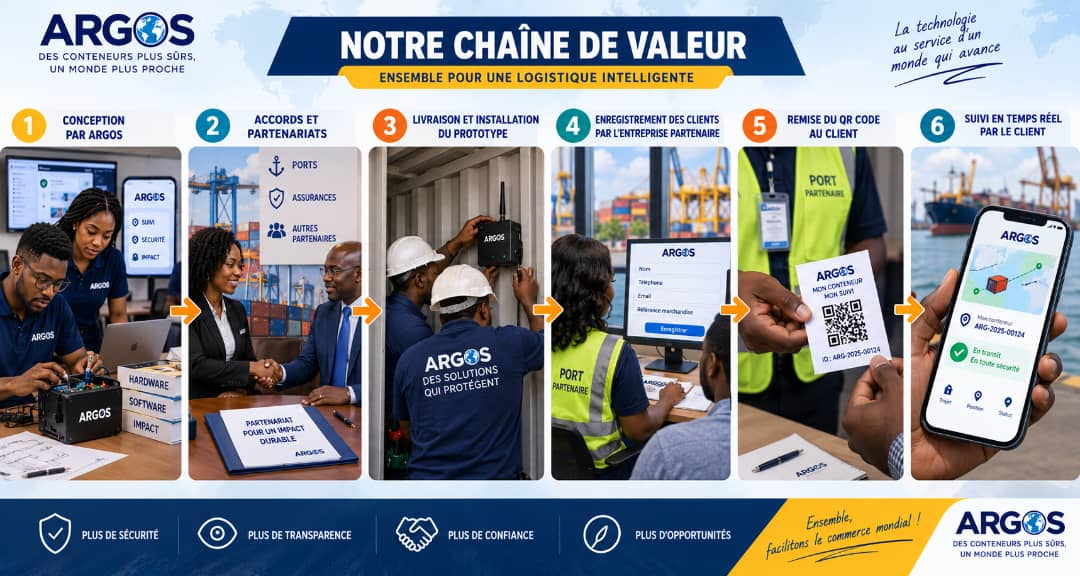
\includegraphics{figures/architecture.jpeg}%
}
\caption{Chaîne de valeur globale et parcours opérationnel ARGOS}
\label{fig-argos-chaine-valeur}
\tablesourcepromoteurs
\end{figure}

Cette architecture visuelle met en lumière les points clés suivants :
\begin{itemize}
    \item \textbf{R\&D et fabrication interne (\textit{Hardware} et \textit{Software}) :} maîtrise initiale de la conception des boîtiers intelligents et des interfaces logicielles par l'équipe technique d'ARGOS.
    \item \textbf{Ancrage partenarial et institutionnel :} formalisation des accords avec les autorités portuaires, les assurances et les acteurs logistiques pour assurer la conformité opérationnelle.
    \item \textbf{Déploiement physique et traçabilité sur le terrain :} installation matérielle autonome des boîtiers connectés à l'intérieur des conteneurs, couplée à un enregistrement rigoureux des profils clients.
    \item \textbf{Sécurisation des accès et supervision en temps réel :} remise d'un identifiant cryptographique unique (QR code) au client final et suivi télématique distant de l'acheminement des marchandises via l'application mobile.
\end{itemize}

En définitive, cette frise valide l'alignement stratégique de la solution autour de quatre piliers fondamentaux : la sécurité matérielle, la transparence des flux, la confiance partenariale et l'optimisation des opportunités logistiques.

\subsubsection{Architecture fonctionnelle}

La figure \ref{fig-architecture-systeme} présente l'architecture fonctionnelle et technique globale du système ARGOS. Ce schéma illustre de manière synthétique l'interaction entre les différentes composantes de la solution, de l'acquisition des données jusqu'à leur restitution.

\begin{figure}[htbp]
    \centering
    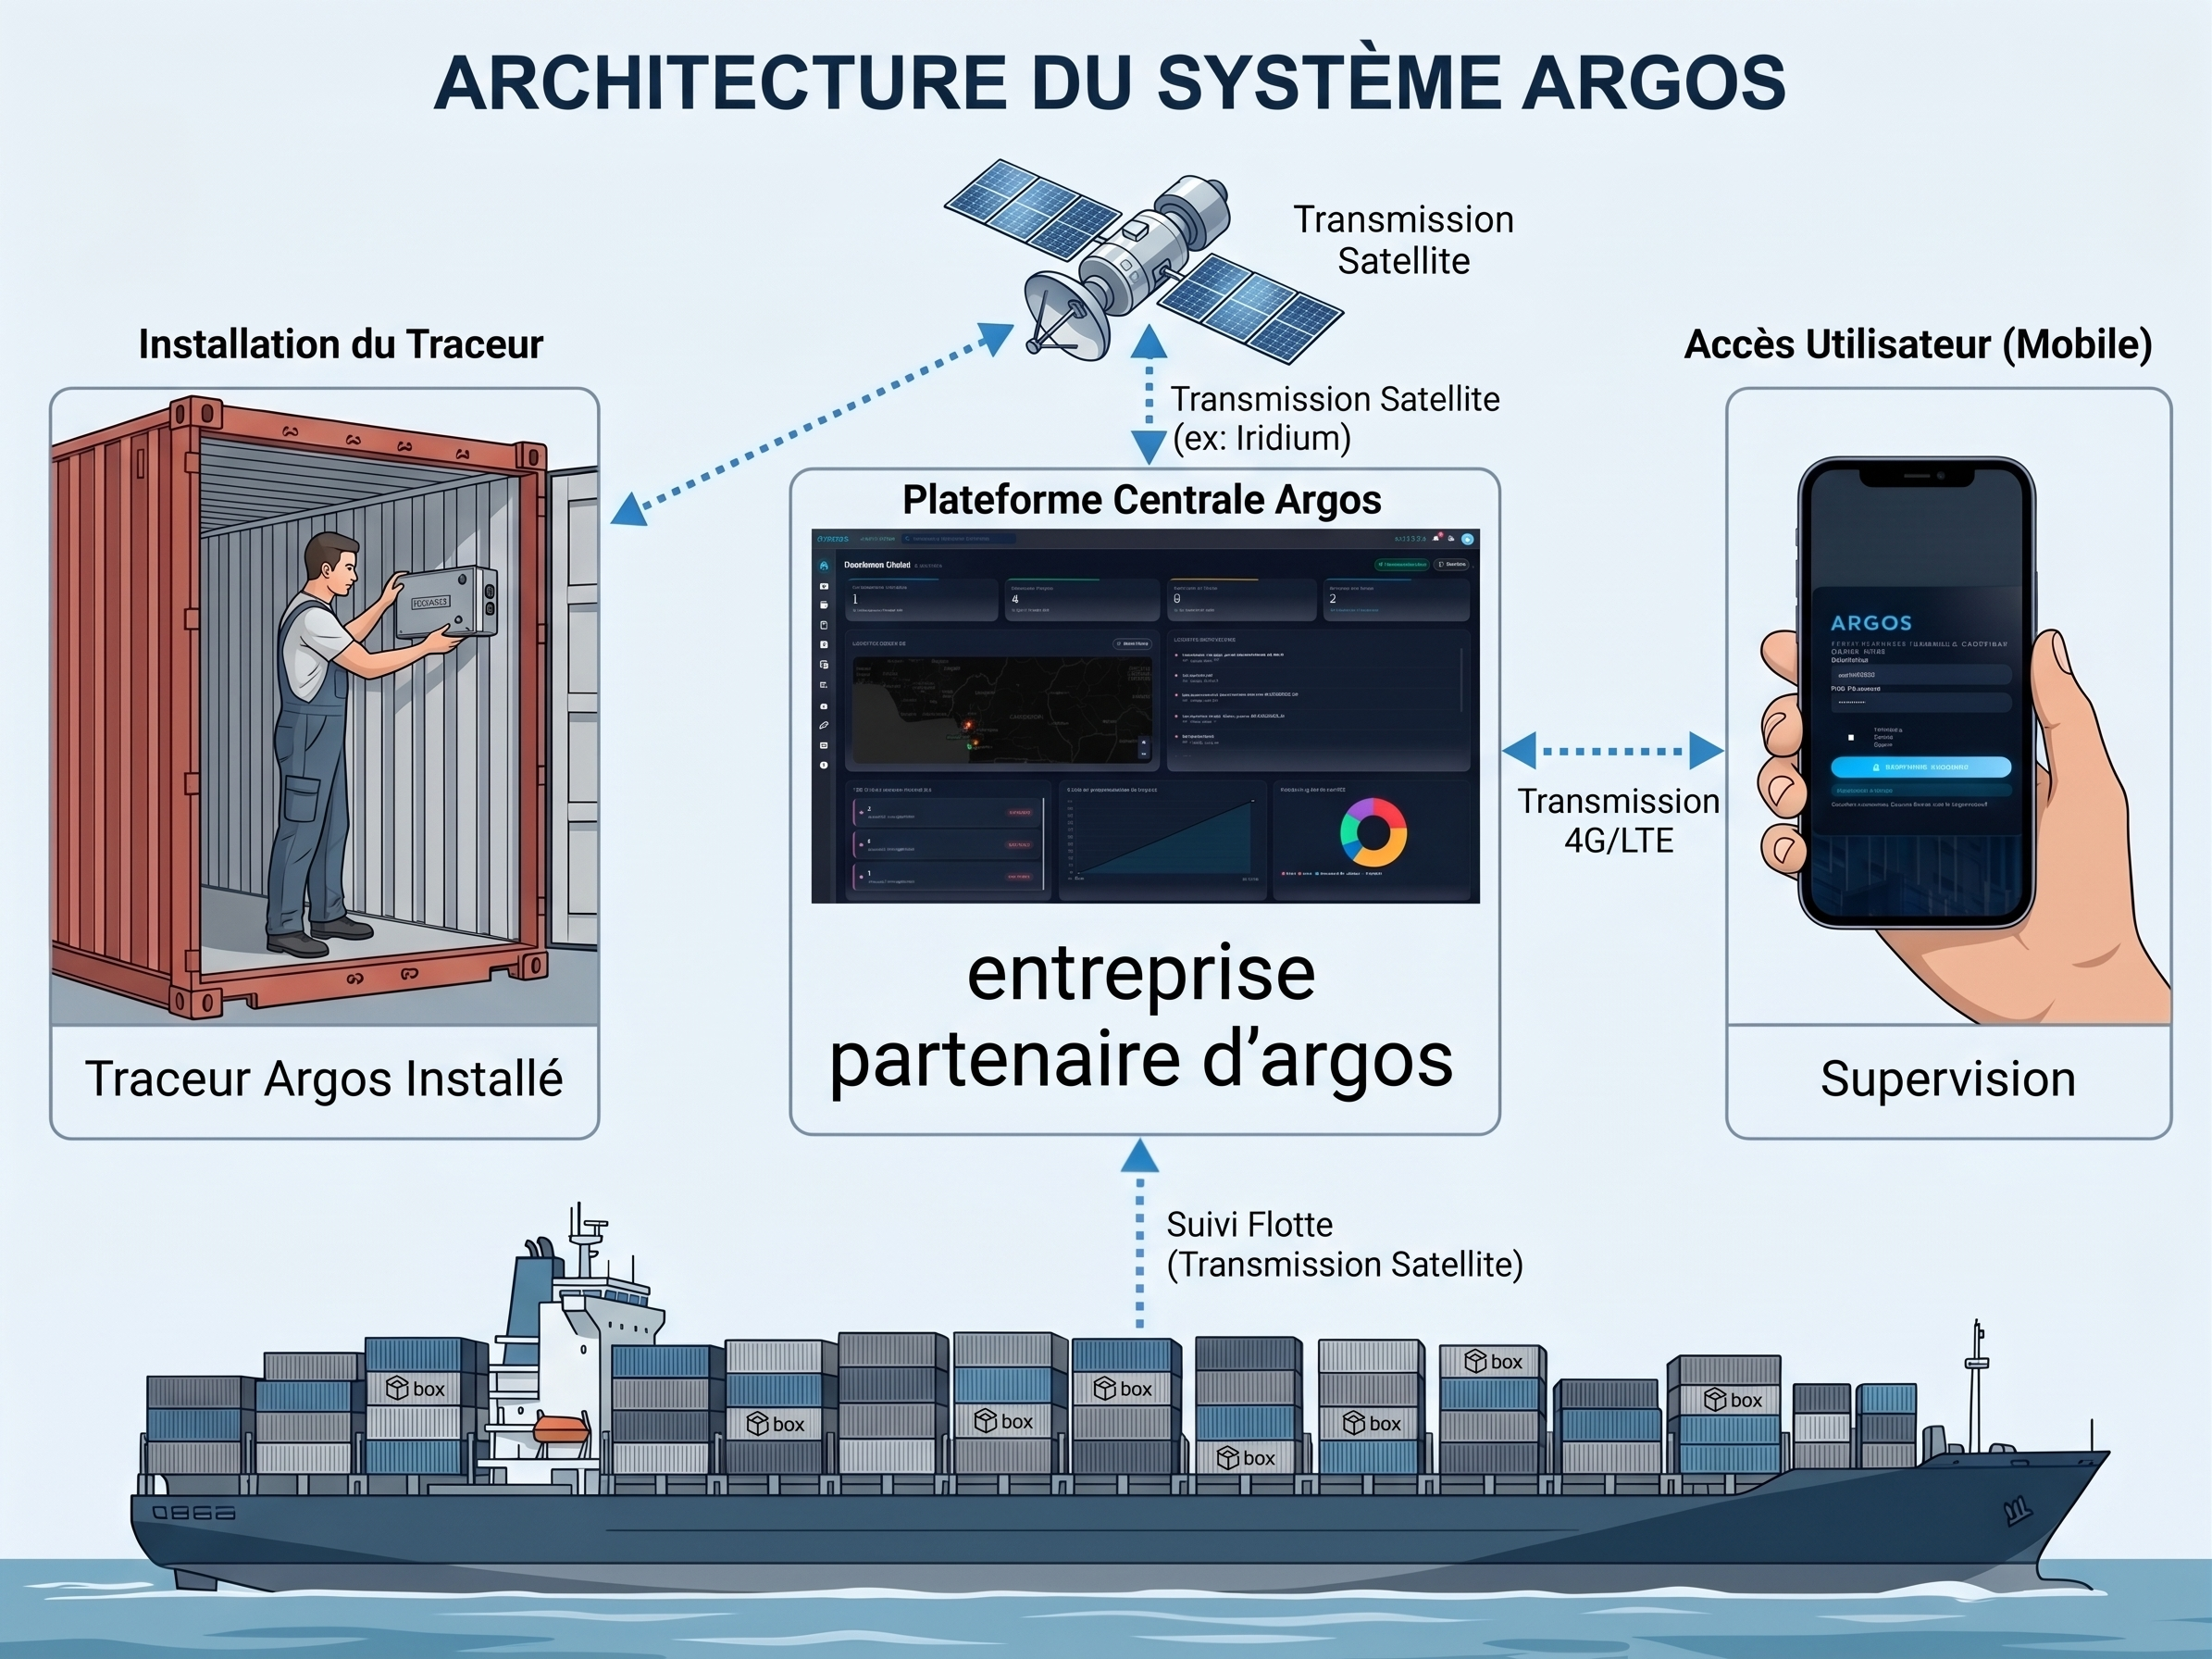
\includegraphics[width=\linewidth,keepaspectratio]{arch.jpeg}
    \caption{Architecture globale et flux de communication du système ARGOS}
    \label{fig-architecture-systeme}
    \tablesourcepromoteurs
\end{figure}

\begin{figure}[htbp]
    \centering
    % Architecture issue du code déployé. Vue volontairement synthétique pour
% rendre visibles les responsabilités et les stockages sans croiser les flux.
\resizebox{\textwidth}{!}{%
\begin{tikzpicture}[
  font=\sffamily\Large,
  client/.style={draw=argosmid,rounded corners=6pt,fill=white,
    text width=8.0cm,minimum height=2.4cm,align=center,line width=1.5pt},
  gateway/.style={draw=argosnavy,rounded corners=6pt,fill=argoslight,
    text width=12.0cm,minimum height=2.8cm,align=center,line width=1.6pt},
  service/.style={draw=argosmid,rounded corners=6pt,fill=argospale,
    text width=8.0cm,minimum height=2.8cm,align=center,line width=1.5pt},
  store/.style={draw=argosnavy,cylinder,shape border rotate=90,aspect=.22,
    fill=white,text width=8.2cm,minimum height=2.9cm,align=center,line width=1.6pt},
  worker/.style={draw=argosnavy,rounded corners=6pt,fill=argoslight,
    text width=8.0cm,minimum height=2.7cm,align=center,line width=1.6pt},
  external/.style={draw=argosrule,rounded corners=6pt,fill=white,
    text width=8.0cm,minimum height=2.4cm,align=center,line width=1.5pt},
  layer/.style={draw=argosrule,rounded corners=8pt,inner sep=10mm,line width=1.5pt},
  title/.style={font=\sffamily\huge\bfseries,text=argosblue,
    fill=white,inner sep=5pt},
  flow/.style={draw=argosgray,line width=1.6pt,-{Stealth[length=4.5mm]}},
  bidir/.style={draw=argosgray,line width=1.6pt,
    {Stealth[length=4.5mm]}-{Stealth[length=4.5mm]}},
  async/.style={draw=argosmid,dashed,line width=1.6pt,-{Stealth[length=4.5mm]}},
  bus/.style={draw=argosgray,line width=1.6pt},
  edgeLabel/.style={font=\sffamily\Large\bfseries,fill=white,inner sep=3pt,align=center}
]

% 1. Canaux d'acquisition.
\node[client] (web) at (-16.0,16.0)
  {Navigateur ARGOS\\Jinja, HTML/CSS et JavaScript};
\node[client] (station) at (0,16.0)
  {ESP32 en mode station\\HTTP REST + \texttt{X-Device-Key}};
\node[client] (ap) at (16.0,16.0)
  {ESP32 en point d'accès\\API locale \texttt{192.168.4.1}};
\node[layer,fit=(web)(station)(ap)] (clients) {};
\node[title] at (0,18.3) {CLIENTS ET CANAUX D'ACQUISITION};

% 2. Façades HTTP et contrôles.
\node[gateway] (webapi) at (-9.5,10.2)
  {Flask / Gunicorn et 12 blueprints\\API métier, Bearer signé, rôle et périmètre};
\node[gateway] (iotapi) at (9.5,10.2)
  {Contrôleurs IoT\\clé technique, enrôlement, télémétrie, audio, commandes et pont direct};
\node[layer,fit=(webapi)(iotapi)] (gateways) {};
\node[title] at (0,12.5) {COUCHE HTTP ET CONTRÔLE D'ACCÈS};

% 3. Services du monolithe.
\node[service] (business) at (-17.5,3.8)
  {Logistique et comptes\\conteneurs, boîtes, BIC, maritime et workflows};
\node[service] (iot) at (-5.8,3.8)
  {Pipeline IoT commun\\validation, liaison, séquence, qualité et seuils};
\node[service] (projection) at (5.8,3.8)
  {Projection applicative\\carte, boîtes, statistiques, alertes et événements};
\node[service] (documents) at (17.5,3.8)
  {Documents et diffusion\\PDF, QR, notifications internes et e-mail};
\node[layer,fit=(business)(iot)(projection)(documents)] (services) {};
\node[title] at (0,6.2) {SERVICES MÉTIER DU MONOLITHE MODULAIRE};

% 4. Données et traitement différé.
\node[store] (postgres) at (-16.5,-3.5)
  {PostgreSQL / TimescaleDB\\schéma \texttt{brady} : métier, mesures, positions, événements, audit et tâches};
\node[worker] (worker) at (-5.5,-3.5)
  {Worker Python\\verrouille \texttt{background\_jobs} dans PostgreSQL};
\node[store] (redis) at (6.0,-3.5)
  {Redis\\DB0 : limitation de débit\\DB1 : \texttt{latest} + stream IoT};
\node[store] (private) at (17.5,-3.5)
  {Volume privé persistant\\audio, contrats, inventaires et rapports};
\node[layer,fit=(postgres)(worker)(redis)(private)] (data) {};
\node[title] at (0,-0.8) {DONNÉES ET TRAITEMENTS DIFFÉRÉS};

% 5. Adaptateurs externes.
\node[external] (providers) at (-17.5,-10.5)
  {BIC BoxTech et fournisseur maritime\\adaptateurs configurables};
\node[external] (transport) at (-5.8,-10.5)
  {Transport de commandes\\HTTP ; MQTT/TLS optionnel};
\node[external] (tunnel) at (5.8,-10.5)
  {Cloudflare Tunnel\\publication HTTPS distante};
\node[external] (mail) at (17.5,-10.5)
  {SMTP / Infobip\\e-mail ; WhatsApp optionnel};
\node[layer,fit=(providers)(transport)(tunnel)(mail)] (externals) {};
\node[title] at (0,-8.0) {SYSTÈMES EXTERNES ET ADAPTATEURS};

% Entrées : le point d'accès est lu par le navigateur, jamais par le VPS.
\draw[flow] (web.south) -- node[edgeLabel,right]{HTTPS / JSON} (webapi.north west);
\draw[flow] (station.south) -- node[edgeLabel,right]{\texttt{/api/iot/*}} (iotapi.north west);
\draw[flow] (ap.south) -- ++(0,-0.85) -| node[edgeLabel,pos=.15,below]{lecture locale HTTP} (web.south east);
\draw[flow] (webapi.east) -- node[edgeLabel,above]{pont direct authentifié} (iotapi.west);

% Les deux façades distribuent vers un bus de services internes.
\draw[flow] (webapi.south) -- (-9.5,5.6);
\draw[flow] (iotapi.south) -- (9.5,5.6);
\draw[bus] (-17.5,5.6) -- (17.5,5.6);
\draw[flow] (-17.5,5.6) -- (business.north);
\draw[flow] (-5.8,5.6) -- (iot.north);
\draw[flow] (5.8,5.6) -- (projection.north);
\draw[flow] (17.5,5.6) -- (documents.north);

% Persistance et temps réel.
\draw[bidir] (business.south) -- node[edgeLabel,right]{métier} (postgres.north west);
\draw[flow] (iot.south west) -- node[edgeLabel,left]{durable} (postgres.north east);
\draw[bidir] (iot.south east) -- node[edgeLabel,left]{cache + stream} (redis.north west);
\draw[bidir] (projection.south) -- node[edgeLabel,right]{Redis d'abord} (redis.north);
\draw[bidir] (documents.south) -- (private.north);
\draw[bidir] (worker.west) -- node[edgeLabel,above]{\texttt{SKIP LOCKED}} (postgres.east);

\node[font=\sffamily\Large,text=argosgray,align=center] at (0,-13.2)
  {Figure~\ref{fig-argos-architecture} : architecture logicielle de la solution ARGOS.};
\end{tikzpicture}%
}
    \caption{Architecture logicielle}
    \label{fig-argos-architecture}
    \tablesourcepromoteurs

\end{figure}

La \cref{fig-argos-architecture} détaille la structure interne d'ARGOS sous la forme d'un monolithe modulaire organisé en cinq couches fonctionnelles superposées. Cette découpe assure une séparation stricte entre les réseaux d'acquisition, le contrôle d'accès, la logique métier, la persistance hybride et les intégrations tierces.

\paragraph{Clients et canaux d'acquisition.}
L'accès à la plateforme s'effectue via trois canaux complémentaires. Le navigateur web charge l'interface dynamique et consomme les API distantes. Sur le terrain, l'ESP32-S3 transmet sa télémétrie au serveur distant en mode station via le protocole HTTP REST sécurisé par la clé \code{X-Device-Key}. En mode point d'accès (\code{192.168.4.1}), le boîtier expose une API locale directement interrogeable par le navigateur client, qui agit alors comme un pont applicatif contrôlé entre le sous-réseau local du matériel et la plateforme ARGOS.

\paragraph{Couche HTTP et contrôle d'accès.}
La façade d'entrée est opérée par Gunicorn exécutant la fabrique d'application Flask, découpée en 12 \emph{blueprints}. Un filtre d'authentification centralisé intercepte l'ensemble des routes sous \code{/api/}, exigeant un jeton Bearer signé ainsi qu'une vérification stricte du rôle et du périmètre de l'utilisateur. En parallèle, les contrôleurs IoT gèrent l'enrôlement, la validation des clés techniques, l'ingestion de la télémétrie, le flux audio, l'émission des commandes et la session du pont direct.

\paragraph{Services métier du monolithe modulaire.}
La logique applicative regroupe quatre domaines fondamentaux à savoir :
\begin{itemize}
    \item \textbf{Logistique et comptes :} gestion du parc de conteneurs, des boîtes noires, intégration des normes BIC/BoxTech, suivi des trajets maritimes et orchestration des workflows ;
    \item \textbf{Pipeline IoT commun :} validation du contrat JSON, contrôle de séquence, évaluation de la qualité des capteurs et calcul automatique du franchissement des seuils d'alerte ;
    \item \textbf{Projection applicative :} agrégation temps réel pour la cartographie, suivi de l'état des boîtes, calcul des indicateurs statistiques et génération des événements ;
    \item \textbf{Documents et diffusion :} création automatique des rapports PDF, génération des QR codes, diffusion des notifications internes et expédition des courriels.
\end{itemize}

\paragraph{Données et traitements différés.}
La persistance repose sur une architecture hybride optimisée :
\begin{itemize}
    \item \textbf{Redis (Multi-DB) :} la base DB0 assure la limitation de débit (\emph{rate limiting}) pour prémunir le serveur contre les dénis de service, tandis que la base DB1 conserve l'instantané de la dernière mesure (\emph{latest}, durée de vie de 24 heures) et le flux tampon (\emph{stream}) borné à environ $10\,000$ entrées pour un affichage dynamique à très faible latence ;
    \item \textbf{PostgreSQL / TimescaleDB (Schéma \code{argos}) :} constitue la source de vérité durable pour l'ensemble des entités métier, lectures de capteurs, positions GPS, événements, journaux d'audit et tâches d'arrière-plan ;
    \item \textbf{Worker Python :} dépile et exécute de façon sécurisée les tâches différées (\code{background\_jobs}) enregistrées en base au moyen du verrouillage SQL \code{SKIP LOCKED} ;
    \item \textbf{Volume privé persistant :} garantit le stockage isolé des fichiers sensibles (segments audio, contrats PDF, inventaires et rapports) hors du répertoire statique public.
\end{itemize}

\paragraph{Systèmes externes et adaptateurs.}
La couche inférieure regroupe les connecteurs d'intégration : les adaptateurs BIC BoxTech et maritimes pour la normalisation du suivi, le transport HTTP/MQTT pour l'exécution distante des commandes, l'exposition distante sécurisée via Cloudflare Tunnel (HTTPS/HTTP2) sans ouverture directe des ports du routeur, ainsi que les passerelles SMTP et Infobip pour la diffusion des alerteurs par courriel ou WhatsApp.

\subsubsection{Organisation des modules}

\begin{longtable}{@{}p{3.2cm}p{5.6cm}p{6.2cm}@{}}
\caption{Organisation des douze blueprints Flask}
\label{tab-blueprints-argos}\\
\tableheadrow \thc{Blueprint} & \thc{Routes principales} & \thc{Responsabilités} \\
\midrule
\endfirsthead
\tableheadrow \thc{Blueprint} & \thc{Routes principales} & \thc{Responsabilités} \\
\midrule
\endhead
\code{auth} & \code{/api/login}, \code{/api/auth/*} & Connexion, disponibilité du login et changement du mot de passe \\
\hline
\code{dashboard} & \code{/}, \code{/api/stats*}, \code{/api/dashboard/*} & Page principale, KPI, statistiques historiques et temps réel \\
\hline
\code{containers} & \code{/api/containers/*}, \code{/api/notifications} & Parc de conteneurs, positions, vente, inventaire et notification \\
\hline
\code{black\_boxes} & \code{/api/black-boxes/*} & Création, QR, affectation, reconnexion, session directe, rapport et archivage \\
\hline
\code{boites\_noires} & \code{/api/boites-noires/*}, \code{/api/captive/*} & Compatibilité historique et parcours du portail captif \\
\hline
\code{telemetry} & \code{/api/telemetry}, \code{/api/config/thresholds}, \code{/api/events} & Compatibilité de télémétrie, seuils, monitoring et événements \\
\hline
\code{iot} & \code{/api/iot/*}, \code{/api/black-boxes/*/commands/*} & Enrôlement, ingestion, audio, commandes, acquittements et mode sécurité \\
\hline
\code{users} & \code{/api/companies}, \code{/api/clients}, \code{/api/drivers} & Comptes, entreprises, clients, chauffeurs et abonnements \\
\hline
\code{workflows} & \code{/api/contracts/*}, \code{/api/documents}, \code{/api/destocking/*} & Contrats, inventaires, documents, vote et déstockage \\
\hline
\code{maritime} & \code{/api/container/validate}, \code{/api/voyage/*}, \code{/api/litiges} & BIC, voyages, tracking et contrôles portuaires \\
\hline
\code{blockchain} & \code{/api/blockchain/*} & Consultation, statistiques et vérification du journal d'événements \\
\hline
\code{publication} & \code{/api/publications} & Création et consultation des publications \\
\tablebottomrule
\end{longtable}
\tablesourcepromoteurs

\subsection{Organigramme de l'application}

\begin{figure}[H]
    \centering
    \resizebox{\textwidth}{!}{% Force le schéma à tenir dans la largeur de la page
        \resizebox{\textwidth}{!}{%
\begin{tikzpicture}[
  font=\sffamily\small,
  start/.style={draw=argosnavy,rounded corners=8pt,fill=argoslight,
    text width=4.8cm,minimum height=1.3cm,align=center,line width=1pt},
  action/.style={draw=argosmid,rounded corners=4pt,fill=white,
    text width=4.8cm,minimum height=1.3cm,align=center,line width=.9pt},
  decision/.style={draw=argosnavy,diamond,aspect=2.2,fill=argospale,
    text width=3.4cm,minimum height=1.6cm,align=center,line width=1pt},
  module/.style={draw=argosrule,rounded corners=4pt,fill=argospale,
    text width=3.8cm,minimum height=1.4cm,align=center,line width=.9pt},
  api/.style={draw=argosblue,rounded corners=4pt,fill=argoslight,
    text width=6.5cm,minimum height=1.3cm,align=center,line width=1pt},
  flow/.style={draw=argosgray,line width=1pt,-{Stealth[length=3mm]}},
  label/.style={font=\sffamily\scriptsize\bfseries,fill=white,inner sep=2pt}
]

% 1. Authentification & Connexion
\node[start] (open) at (0,12.0) {Ouverture de l'application ARGOS};
\node[decision] (token) at (0,9.5) {Jeton signé valide ?};
\node[action] (login) at (-7.5,9.5) {Saisir le login et le mot de passe};
\node[decision] (credentials) at (-7.5,6.8) {Identifiants valides ?};
\node[action] (reject) at (-13.5,6.8) {Refus, message d'erreur};

% 2. Validation & Chargement du Périmètre
\node[decision] (contract) at (0,6.8) {Contrat en attente ?};
\node[action] (accept) at (-6.8,3.8) {Lire, télécharger et décider};
\node[action] (scope) at (0,3.8) {Charger le rôle et le périmètre\\de ressources autorisées};
\node[action] (nav) at (0,1.0) {Construire le menu du profil\\et ouvrir le tableau de bord};

% Flux d'authentification
\draw[flow] (open) -- (token);
\draw[flow] (token.west) -- node[label,above]{non} (login.east);
\draw[flow] (login) -- (credentials);
\draw[flow] (credentials.west) -- node[label,above]{non} (reject.east);
\draw[flow] (reject.north) |- (login.west);
\draw[flow] (credentials.east) -- node[label,above]{oui} (contract.west);
\draw[flow] (token) -- node[label,right]{oui} (contract);
\draw[flow] (contract.south west) -- node[label,above,sloped]{oui} (accept.north east);
\draw[flow] (accept.east) -- node[label,above]{accepté} (scope.west);
\draw[flow] (contract) -- node[label,right]{non} (scope);
\draw[flow] (scope) -- (nav);

% 3. Modules Applicatifs (Espacement horizontal de 4.4cm)
\node[module] (dash) at (-11.0,-2.0) {Tableau de bord\\KPI et état du parc};
\node[module] (map) at (-6.6,-2.0) {Carte et conteneurs\\positions, trajets, détails};
\node[module] (boxes) at (-2.2,-2.0) {Boîtes noires\\QR, affectation, connexion};
\node[module] (stats) at (2.2,-2.0) {Statistiques\\filtres et séries temporelles};
\node[module] (events) at (6.6,-2.0) {Événements et alertes\\tri, lecture, notifications};
\node[module] (docs) at (11.0,-2.0) {Documents et workflows\\contrats, inventaire, déstockage};

\foreach \target in {dash,map,boxes,stats,events,docs}
  \draw[flow] (nav.south) -- ++(0,-1.0) -| (\target.north);

% 4. Contrôle de Rôle & Actions Métier
\node[decision] (manager) at (-5.0,-5.2) {Gestionnaire autorisé ?};
\node[action] (direct) at (-10.5,-8.2) {Mode direct : vérifier \texttt{deviceUid},\\lire l'AP et synchroniser la file};
\node[action] (security) at (-5.0,-8.2) {Activer ou bloquer la sécurité\\et auditer l'auteur};
\node[action] (consult) at (3.5,-8.2) {Consultation filtrée selon\\rôle, boîte et conteneur};

% Flux métiers
\draw[flow] (boxes.south) |- (manager.north);
\draw[flow] (manager.south west) -- node[label,above,sloped]{oui} (direct.north east);
\draw[flow] (manager) -- node[label,right]{oui} (security);
\draw[flow] (map.south) |- (consult.north);
\draw[flow] (stats.south) |- (consult.north);
\draw[flow] (events.south) |- (consult.north);
\draw[flow] (docs.south) |- (consult.north);
\draw[flow] (manager.east) -- node[label,above]{non} (consult.west);

% 5. API Backend & Rendu Final
\node[api] (api) at (0,-11.2) {Appel API avec jeton Bearer\\contrôle rôle + propriété de la ressource};
\node[action] (data) at (0,-13.8) {Lecture Redis temps réel ou PostgreSQL\\puis rendu carte, boîtes, statistiques et événements};

\draw[flow] (direct.south) |- (api.west);
\draw[flow] (security.south) -- (api.north west);
\draw[flow] (consult.south) -- (api.north east);
\draw[flow] (api) -- (data);

\end{tikzpicture}%
}
    }
    \caption{Organigramme fonctionnel de navigation et de contrôle d'accès}
    \label{fig-argos-organigramme-application}
    \tablesourcepromoteurs
\end{figure}

L'organigramme de la \cref{fig-argos-organigramme-application} montre que le
menu n'est pas une preuve d'autorisation. Il améliore l'ergonomie en masquant
les pages étrangères au rôle, tandis que les principales API privées
recalculent le périmètre des boîtes et conteneurs autorisés. Le
superadministrateur reçoit le périmètre
global ; les autres profils reçoivent une liste issue des liens de propriété,
d'agence, d'abonnement, de transport ou de port.

\section{Conception détaillée}

Cette section approfondit les choix de conception présentés précédemment en entrant dans le détail technique de leur mise en œuvre. Elle décrit notamment l'architecture matérielle du prototype, les mécanismes de sécurité mis en place ainsi que la modélisation du système à travers différents diagrammes. Elle a pour but de montrer concrètement comment les orientations générales du projet se traduisent en solutions techniques précises et réalisables.

\subsection{Architecture du prototype ESP32}

L'ESP32 est un microcontrôleur à faible consommation d'énergie, doté d'une connectivité Wi-Fi et Bluetooth intégrée, largement utilisé dans les projets d'objets connectés (IoT). Il permet de piloter divers capteurs et modules de communication tout en assurant le traitement local des données. Cette section présente l'architecture du prototype ARGOS construite autour de ce composant, en détaillant le raccordement matériel des différents éléments ainsi que le fonctionnement du micrologiciel qui les pilote.

\subsubsection{Raccordement matériel}

Cette section décrit la manière dont les différents composants électroniques du prototype ARGOS sont physiquement reliés au microcontrôleur ESP32. Elle précise pour chaque élément capteurs, module de communication, module GPS, carte mémoire, alarme et indicateurs lumineux la broche à laquelle il est connecté ainsi que la fonction qu'il assure. Cette présentation permet de comprendre l'organisation matérielle du dispositif avant d'aborder le fonctionnement logiciel qui l'exploite.

\begin{table}[htbp]
\centering
\caption{Affectation des broches du micrologiciel ARGOS}
\label{tab-broches-esp32}
\begin{tabularx}{\textwidth}{@{}p{3.5cm}p{2.2cm}X@{}}
\tableheadrow \thc{Élément} & \thc{GPIO} & \thc{Fonction} \\
\midrule
LED bleue & 1 & Témoin d'alimentation et de fonctionnement, maintenu allumé en permanence \\
\hline
Bouton BOOT & 0 & Appui de trois secondes pour revenir au mode de configuration \\
\hline
Photorésistance LDR & 3 & Niveau lumineux et contribution à la détection d'ouverture \\
\hline
AM2302/DHT22 & 4 & Température et humidité \\
\hline
Microphone analogique & 5 & Niveau sonore \\
\hline
HC-SR04 & 6 / 7 & Déclenchement et écho de la mesure de distance \\
\hline
MPU6050 & 8 / 9 & Bus I\textsuperscript{2}C SDA/SCL, accélérations et choc \\
\hline
Buzzer & 10 & Alarme locale \\
\hline
Carte microSD & 11 / 12 / 13 / 14 & SPI MOSI, SCK, MISO et CS pour le journal local \\
\hline
SIM800 & 15 / 16 & UART prévu pour la communication cellulaire \\
\hline
GPS NEO-6M & 17 / 18 & UART de localisation \\
\hline
Capteur de flamme & 21 & Détection numérique de flamme \\
\hline
LED RGB intégrée & 48 par défaut & État visuel complémentaire de la carte ESP32-S3 \\
\tablebottomrule
\end{tabularx}
\tablesourcepromoteurs
\end{table}

\subsubsection{Cycle de vie du micrologiciel}

Au démarrage, le micrologiciel initialise les entrées/sorties, teste les LED,
interroge le DHT22, le MPU6050 et la carte SD, puis charge les paramètres
conservés dans \code{Preferences}. Le \code{deviceUid} est dérivé de l'eFuse
si aucune identité n'existe encore. Les numéros de séquence sont réservés par
blocs de 64 afin de rester monotones après un redémarrage sans user la mémoire
flash à chaque mesure.

Si le Wi-Fi, l'URL d'API ou l'identité de boîte manquent, ou après trois
échecs de connexion, l'ESP32 crée le réseau
\code{ARGOS-SETUP-...}. Son serveur local expose :
\begin{itemize}
    \item \code{GET /api/device/info} pour l'identité et les modes ;
    \item \code{GET /api/v1/telemetry} pour le dernier instantané ;
    \item \code{POST /api/v1/security} pour le mode de sécurité local ;
    \item \code{POST /api/v1/provision} pour recevoir la configuration ;
    \item \code{POST /api/v1/register} pour le parcours captif historique.
\end{itemize}

En mode station, l'appareil s'enrôle si sa clé permanente est absente, vérifie
les commandes toutes les cinq secondes et transmet normalement une mesure
toutes les trente secondes. Une nouvelle alarme provoque un envoi anticipé.
Le buzzer dépend du mode sécurité, de la distance, des seuils locaux et de la
détection de flamme. Le mode porte est initialement bloqué et ne peut être
activé que par un gestionnaire autorisé dans l'application.

\subsection{Sécurité et restrictions d'accès}

Cette section présente les mécanismes mis en place pour protéger l'accès à la plateforme ARGOS et contrôler les actions que peut effectuer chaque utilisateur. Elle aborde successivement l'authentification des utilisateurs, la gestion des jetons de session et les règles qui déterminent les droits accordés selon le profil. L'objectif est de garantir que seules les personnes autorisées puissent consulter ou modifier les données sensibles du système.

\subsubsection{Authentification humaine}

Après vérification du hash Werkzeug du mot de passe, ARGOS émet un jeton
Bearer signé et horodaté au moyen de
\code{itsdangerous.URLSafeTimedSerializer}. Il ne s'agit pas d'un JWT. Sa
durée maximale est de 28\,800 secondes par défaut. Il contient le rôle,
l'identifiant, le login, le nom affiché, la portée et la
\code{token\_version}. Le registre \code{identity\_registry} garantit
l'unicité du login entre les familles de comptes et permet de révoquer les
sessions après un changement de mot de passe ou une désactivation.

Les en-têtes historiques \code{X-Role} et \code{X-User-Id} sont ignorés comme
preuves d'identité. Un compte dont le contrat est en attente reçoit une portée
limitée aux routes de consultation et de décision du contrat.

\subsubsection{Authentification du dispositif}

Le provisionnement crée un \code{deviceUid}, un jeton d'enrôlement temporaire
et l'association à une boîte. Seule l'empreinte du jeton est conservée.
L'enrôlement retourne une clé permanente affichée une seule fois ; son hash
est stocké dans \code{iot\_devices}. Une télémétrie distante n'est acceptée
que si la clé, l'état \code{ACTIVE}, la boîte, le conteneur et la séquence
correspondent.

En mode direct, la clé permanente n'est jamais remise au navigateur. Le
navigateur présente son jeton humain au serveur et ARGOS exige l'égalité
exacte entre l'UID lu sur \code{192.168.4.1} et celui associé à la boîte.

\subsubsection{Matrice synthétique des autorisations}

\begin{table}[htbp]
\centering
\small
\caption{Droits fonctionnels principaux par profil}
\label{tab-matrice-roles}
\begin{tabularx}{\textwidth}{@{}p{3.0cm}*{6}{>{\centering\arraybackslash}X}@{}}
\tableheadrow \thc{Fonction} & \thc{Super-admin} & \thc{Proprié-taire} & \thc{Entreprise} & \thc{Client} & \thc{Transpor-teur} & \thc{Autorité portuaire} \\
\midrule
Voir le parc autorisé & Global & Propre & Délégué & Abonné & Mission & Port \\
\hline
Créer/affecter une boîte & Oui & Propre parc & Non & Non & Non & Non \\
\hline
Connexion directe ESP32 & Oui & Propre parc & Déléguée & Non & Non & Non \\
\hline
Activer/bloquer la sécurité & Oui & Propre parc & Déléguée & Non & Non & Non \\
\hline
Statistiques et événements & Global & Propre parc & Délégués & Liés & Liés & Port \\
\hline
Gérer comptes et abonnements & Oui & Clients et chauffeurs liés & Clients liés & Non & Non & Non \\
\hline
Contrôle maritime et douanier & Oui & Consult. & Consult. & Consult. liée & Consult. liée & Oui \\
\tablebottomrule
\end{tabularx}
\tablesourcepromoteurs
\end{table}

\subsection{Diagramme de classes}

Le diagramme de la \cref{fig-argos-classes} expose la vue conceptuelle des entités métiers qui composent la plateforme ARGOS. Cette modélisation UML s'attache à traduire la logique métier du système indépendamment de sa mise en œuvre logicielle, l'implémentation effective s'appuyant sur des services applicatifs et des requêtes SQL optimisées.

La conception statique de la plateforme repose sur un principe fondamental de découplage entre le conteneur logistique, la boîte noire logicielle et le dispositif matériel (ESP32). Cette séparation garantit une grande flexibilité opérationnelle : la réaffectation d'une boîte noire à un nouveau conteneur ou le remplacement d'un composant électronique défectueux s'effectuent sans discontinuité et sans altération de la traçabilité historique des mesures.

Afin d'assurer la cohérence globale des données et de faciliter la maintenance de l'application, le domaine métier est structuré autour de quatre agrégats majeurs :

\begin{itemize}
    \item \textbf{Agrégat 1 : Identités et Organisations :} Il constitue le socle de la gestion des accès et de la confidentialité. Cet agrégat regroupe la définition des profils utilisateurs, la résolution centralisée des rôles applicatifs et la délimitation stricte du périmètre de visibilité des parties prenantes sur les ressources du parc.
    
    \item \textbf{Agrégat 2 : Logistique et Workflows :} Il orchestre l'ensemble du cycle de vie opérationnel. Il régit la traçabilité des conteneurs, le suivi temporel des affectations de boîtes noires et la gouvernance des processus métiers complexes, notamment les procédures collaboratives de déstockage.
    
    \item \textbf{Agrégat 3 : Dispositifs et Télémétrie :} Il encadre la chaîne d'acquisition de données issues du terrain. Cet agrégat assure l'identification unique du matériel embarqué, la réception des messages bruts ainsi que leur transformation en observations physiques qualifiées (température, humidité, chocs) et en coordonnées de géolocalisation.
    
    \item \textbf{Agrégat 4 : Exploitation et Audit :} Il garantit la réactivité du système et l'immuabilité de la preuve. Il prend en charge la détection d'anomalies, la diffusion ciblée des alertes, le scellement de sécurité des événements critiques et la journalisation systématique des actions d'exploitation.
\end{itemize}

La correspondance détaillée entre ces concepts fonctionnels et la structure des tables physiques actuellement déployées en base de données est synthétisée dans le \cref{tab-correspondance-classes}.

\begin{table}[htbp]
\centering
\small
\caption{Correspondance entre agrégats métiers et tables de la base de données}
\label{tab-correspondance-classes}
\begin{tabularx}{\textwidth}{@{}p{4.0cm}p{5.0cm}X@{}}
\tableheadrow \thc{Agrégat} & \thc{Tables centrales} & \thc{Portée fonctionnelle} \\
\midrule
Identités \& Organisations & \code{identity\_registry}, tables de profils & Authentification, contrôle d'accès basé sur les rôles et périmètres de visibilité. \\
\hline
Logistique \& Workflows & \code{conteneurs}, \code{boite\_noir}, \code{assignments}, \code{destocking\_requests} & Gestion du parc, traçabilité des liaisons et suivi des processus d'approbation. \\
\hline
Dispositifs \& Télémétrie & \code{iot\_devices}, \code{iot\_raw\_messages}, \code{sensor\_readings}, \code{positions} & Registre du matériel, ingestion des paquets bruts et persistance des séries temporelles. \\
\hline
Exploitation \& Audit & \code{evenement\_save}, \code{notifications}, \code{audit\_logs}, \code{blockchain\_argos} & Traitement des alertes, traçabilité des opérations et scellement d'intégrité. \\
\tablebottomrule
\end{tabularx}
\tablesourcepromoteurs
\end{table}

\begin{figure}[htbp]
\centering
\resizebox{0.95\textwidth}{!}{%
  % Diagramme de classes métier ARGOS — Version aérée et lisible
\resizebox{\textwidth}{!}{%
\begin{tikzpicture}[
  font=\sffamily\small,
  uml/.style={draw=argosnavy,line width=1.1pt,rectangle split,
    rectangle split parts=2,align=left,inner sep=6pt,text width=5.0cm,fill=white},
  group/.style={draw=argosrule,dashed,rounded corners=6pt,inner sep=8mm,line width=1.2pt},
  assoc/.style={draw=argosgray,line width=1.1pt},
  dep/.style={draw=argosgray,dashed,line width=1.1pt,-{Stealth[length=3mm]}},
  mult/.style={font=\sffamily\small\bfseries,fill=white,inner sep=2pt},
  title/.style={font=\sffamily\large\bfseries,text=argosblue,fill=white,inner sep=4pt}
]

% ==========================================
% AGRÉGAT 1 — IDENTITÉS ET ORGANISATIONS
% ==========================================
\node[uml] (profile) at (-12,13) {\textbf{ProfilActeur}
  \nodepart{second}\texttt{idActeur : String}\\\texttt{rôle : Rôle}\\\texttt{login : String}};

\node[uml] (identity) at (-4,13) {\textbf{Identité}
  \nodepart{second}\texttt{actorRole : String}\\\texttt{actorId : String}\\\texttt{displayName : String}};

\node[uml] (party) at (4,13) {\textbf{PartieLogistique}
  \nodepart{second}\texttt{type : RôleMetier}\\\texttt{périmètre : List<Boîte>}};

\node[group,fit=(profile)(identity)(party),label={[title]above:AGRÉGAT 1 — IDENTITÉS ET ORGANISATIONS}] {};

\draw[assoc] (profile) -- node[mult,near start,above]{1} node[mult,near end,above]{1} (identity);
\draw[dep] (identity) -- node[mult,above]{résout} (party);


% ==========================================
% AGRÉGAT 2 — LOGISTIQUE ET WORKFLOWS
% ==========================================
\node[uml] (container) at (-12,6.5) {\textbf{Conteneur}
  \nodepart{second}\texttt{idConteneur : String}\\\texttt{type, statut : String}};

\node[uml] (box) at (-4,6.5) {\textbf{BoîteNoire}
  \nodepart{second}\texttt{idBoîte : Integer}\\\texttt{uuidQr : UUID}\\\texttt{statut : Boolean}};

\node[uml] (assignment) at (4,6.5) {\textbf{AffectationBoîteConteneur}
  \nodepart{second}\texttt{assignedAt : DateTime}\\\texttt{detachedAt : DateTime?}};

\node[uml] (destock) at (12,6.5) {\textbf{DemandeDéstockage}
  \nodepart{second}\texttt{requiredApprovals : Int}\\\texttt{statut : String}};

\node[group,fit=(container)(box)(assignment)(destock),
  label={[title]above:AGRÉGAT 2 — LOGISTIQUE ET WORKFLOWS}] {};

\draw[assoc] (container) -- node[mult,near start,above]{1} node[mult,near end,above]{0..1} (box);
\draw[assoc] (box) -- node[mult,near start,above]{1} node[mult,near end,above]{0..*} (assignment);
\draw[assoc] (container) |- ++(0,-2.2) -| node[mult,near end,below]{0..*} (destock);


% ==========================================
% AGRÉGAT 3 — DISPOSITIFS ET TÉLÉMÉTRIE
% ==========================================
\node[uml] (device) at (-12,0) {\textbf{DispositifIoT}
  \nodepart{second}\texttt{deviceUid : String}\\\texttt{statut : String}};

\node[uml] (raw) at (-4,0) {\textbf{MessageBrut}
  \nodepart{second}\texttt{messageId : UUID}\\\texttt{payload : JSON}};

\node[uml] (reading) at (4,0) {\textbf{LectureCapteur}
  \nodepart{second}\texttt{sequence : Integer}\\\texttt{temp, humid, choc}};

\node[uml] (position) at (12,0) {\textbf{Position}
  \nodepart{second}\texttt{latitude, longitude}\\\texttt{measuredAt : DateTime}};

\node[group,fit=(device)(raw)(reading)(position),
  label={[title]above:AGRÉGAT 3 — DISPOSITIFS ET TÉLÉMÉTRIE}] {};

\draw[assoc] (device) -- node[mult,near start,above]{1} node[mult,near end,above]{0..*} (raw);
\draw[assoc] (raw) -- node[mult,near start,above]{1} node[mult,near end,above]{0..1} (reading);
\draw[assoc] (raw) |- ++(0,-2.2) -| node[mult,near end,below]{0..1} (position);


% ==========================================
% AGRÉGAT 4 — EXPLOITATION ET AUDIT
% ==========================================
\node[uml] (event) at (-12,-6.5) {\textbf{Événement}
  \nodepart{second}\texttt{idEventInit : BigInt}\\\texttt{horodatage : DateTime}};

\node[uml] (notification) at (-4,-6.5) {\textbf{Notification}
  \nodepart{second}\texttt{type, message : String}\\\texttt{statut : String}};

\node[uml] (audit) at (4,-6.5) {\textbf{JournalAudit}
  \nodepart{second}\texttt{action, entityType}\\\texttt{createdAt : DateTime}};

\node[uml] (block) at (12,-6.5) {\textbf{BlocScellé}
  \nodepart{second}\texttt{blockHash : String}\\\texttt{eventType : String}};

\node[group,fit=(event)(notification)(audit)(block),
  label={[title]above:AGRÉGAT 4 — EXPLOITATION, AUDIT ET PREUVE}] {};

\draw[dep] (event) -- node[mult,above]{alerte} (notification);
\draw[dep] (event) |- ++(0,-2.2) -| node[mult,below]{scellement} (block);


% ==========================================
% LIAISONS ET INTER-RACCORDEMENTS INTER-AGRÉGATS
% ==========================================
% Lien Identité -> Logistique
\draw[assoc] (party.south) |- ++(0,-1.5) -| node[mult,near end,left]{1..*} (container.north);

% Lien BoîteNoire -> Événement
\draw[assoc] (box.south) -- node[mult,near start,right]{1} node[mult,near end,right]{0..*} (event.north);

% Lien DispositifIoT -> JournalAudit
\draw[dep] (device.south) |- ++(0,-1.5) -| node[mult,near end,right]{audit technique} (audit.north);

\end{tikzpicture}%
}%
}
\caption{Diagramme de classes d'ARGOS}
\label{fig-argos-classes}
\end{figure}
\tablesourcepromoteurs

La lecture directe du diagramme de classes permet de formaliser les règles de gestion fondamentales qui régissent les interactions entre les différents agrégats du système ARGOS :

\paragraph{Agrégat « Identités et Organisations »}
La gouvernance des accès repose sur un couplage strict entre les structures d'authentification et les profils. Ainsi, chaque \texttt{ProfilActeur} possède univoquement \textbf{une et une seule} \texttt{Identité}, laquelle se résout et s'articule directement vers une \texttt{PartieLogistique} par le biais d'une relation de dépendance garantissant la portée des droits.

\paragraph{Agrégat « Logistique et Workflows »}
Le suivi du parc opérationnel est conçu pour être flexible et traçable : un \texttt{Conteneur} peut être équipé d'au maximum \textbf{une} \texttt{BoîteNoire} (ou n'en avoir aucune à un instant donné). Pour assurer la traçabilité historique, chaque \texttt{BoîteNoire} fait l'objet de \textbf{zéro à plusieurs} enregistrements d'affectation (\texttt{AffectationBoîteConteneur}), tandis qu'un \texttt{Conteneur} peut initier et concerner \textbf{plusieurs} processus décisionnels de \texttt{DemandeDéstockage}.

\paragraph{Agrégat « Dispositifs et Télémétrie »}
La chaîne d'acquisition de données s'organise autour d'un flux maîtrisé où chaque \texttt{DispositifIoT} génère continuellement des paquets de type \texttt{MessageBrut}. Chacun de ces messages encapsule à son tour au plus \textbf{une} \texttt{LectureCapteur} qualifiée et \textbf{une} \texttt{Position} géolocalisée.

\paragraph{Agrégat « Exploitation, Audit et Preuve »}
La sécurité et la réactivité du système s'appuient sur des mécanismes de traçabilité événementielle. Par des relations de dépendance ciblées, chaque \texttt{Événement} critique déclenche instantanément une alerte sous forme de \texttt{Notification} et implique un scellement immuable au sein d'un \texttt{BlocScellé}.

\paragraph{Liaisons transversales et inter-agrégats}
Enfin, la cohérence globale de l'écosystème est assurée par des ponts relationnels majeurs : toute \texttt{PartieLogistique} doit piloter et gérer \textbf{au moins un} \texttt{Conteneur}. De son côté, chaque \texttt{BoîteNoire} consigne l'ensemble des anomalies sous forme de \textbf{zéro à plusieurs} \texttt{Événement}s, tandis que chaque \texttt{DispositifIoT} documente rigoureusement son intégrité opérationnelle en traçant son audit technique vers le \texttt{JournalAudit}.


\subsection{Diagramme des cas d'utilisation}
\par La modélisation fonctionnelle du diagramme de cas d'utilisation a pour objectif fondamental de décrire le système du point de vue de ses utilisateurs et des acteurs externes avec lesquels il interagit, en mettant en lumière les services et les fonctionnalités offerts par la plateforme. Pour ce faire, le diagramme de cas d'utilisation UML constitue l'outil de référence : son rôle est d'identifier de manière exhaustive les frontières du système ARGOS, de cartographier les interactions entre chaque profil d'utilisateur (humain ou technique) et de formaliser les exigences comportementales attendues. Afin de restituer fidèlement la complexité opérationnelle et administrative du projet, l'analyse fonctionnelle se décline ci-après à travers deux axes complémentaires : d'une part, les cas d'utilisation administratifs, qui régissent la gouvernance et la gestion du parc, et d'autre part, les cas d'utilisation opérationnels, qui encadrent l'exécution sur le terrain et le suivi télématique.

\subsubsection{Cas d'utilisation administratifs}

La modélisation fonctionnelle d'ARGOS s'articule autour de deux vues complémentaires : d'une part, 
les cas d'utilisation administratifs qui régissent la gouvernance, la configuration du parc et la gestion des comptes ; 
d'autre part, les cas d'utilisation opérationnels qui décrivent l'exécution sur le terrain, 
le suivi télématique direct et les interactions avec les dispositifs embarqués.

\begin{figure}[htbp]
\centering
\begin{minipage}{\textwidth}
\centering
\resizebox{0.82\textwidth}{!}{%
  % Diagramme de cas d'utilisation administratifs — ARGOS (Optimisé & Complet)
\resizebox{\textwidth}{!}{%
\begin{tikzpicture}[
  font=\sffamily\large\bfseries,
  uc/.style={draw=argosmid,ellipse,align=center,text width=5.5cm,
    minimum width=6.0cm,minimum height=1.5cm,fill=white,line width=1.4pt},
  link/.style={draw=argosgray,line width=1.4pt},
  inherit/.style={draw=argosnavy,line width=1.4pt,-{Triangle[open,length=4.5mm]}},
  boundary/.style={draw=argosnavy,rounded corners=8pt,inner sep=10mm,line width=1.8pt},
  actorfont/.style={font=\sffamily\large\bfseries,align=center,text=argosnavy}
]

% -----------------------------------------------------------------
% COMMANDE TIKZ POUR DESSINER UN BONSHOMME UML
% -----------------------------------------------------------------
\newcommand{\drawstickman}[3]{ % #1: name, #2: (x,y), #3: label
  \coordinate (center) at #2;
  \draw[draw=argosnavy,line width=1.5pt,fill=argospale] ($(center)+(0,0.9)$) circle (0.42cm);
  \draw[draw=argosnavy,line width=1.5pt] ($(center)+(0,0.48)$) -- ($(center)+(0,-0.4)$);
  \draw[draw=argosnavy,line width=1.5pt] ($(center)+(-0.5,0.25)$) -- ($(center)+(0.5,0.25)$);
  \draw[draw=argosnavy,line width=1.5pt] ($(center)+(0,-0.4)$) -- ($(center)+(-0.4,-1.0)$);
  \draw[draw=argosnavy,line width=1.5pt] ($(center)+(0,-0.4)$) -- ($(center)+(0.4,-1.0)$);
  \node[actorfont,anchor=north] at ($(center)+(0,-1.15)$) {#3};
  \node[rectangle,inner sep=2pt,minimum width=4.0cm,minimum height=3.0cm] (#1) at ($(center)+(0,0.1)$) {};
}

% -----------------------------------------------------------------
% POSITIONNEMENT DES ACTEURS (Echelle Y compacte pour affichage complet)
% -----------------------------------------------------------------
% Acteur racine
\drawstickman{user}{(-15.0, 1.8)}{Utilisateur Authentifié};

% Acteurs intermédiaires
\drawstickman{company}{(-7.5, 5.5)}{Agence / Entreprise};
\drawstickman{port}{(-7.5, -2.0)}{Autorité Portuaire};

% Acteur spécialisé
\drawstickman{owner}{(-15.0, 9.2)}{Propriétaire};

% Acteur suprême
\drawstickman{admin}{(-15.0, 13.5)}{Superadministrateur};

% -----------------------------------------------------------------
% LIENS D'HÉRITAGE (Sur les bordures externes)
% -----------------------------------------------------------------
\draw[inherit] (company.north west) -- node[above,font=\small\bfseries,sloped]{hérite} (user.north east);
\draw[inherit] (port.north west) -- node[below,font=\small\bfseries,sloped]{hérite} (user.south east);
\draw[inherit] (owner.south) -- node[right,font=\small\bfseries]{hérite} (company.north west);
\draw[inherit] (admin.south) -- node[right,font=\small\bfseries]{hérite} (owner.north);

% -----------------------------------------------------------------
% CAS D'UTILISATION (Disposition en grille verticale équilibrée)
% -----------------------------------------------------------------
% Superadministrateur
\node[uc] (accounts) at (4.0, 13.5) {Gérer entreprises, comptes et rôles globaux};
\node[uc] (audit) at (4.0, 11.2) {Consulter et vérifier les données scellées};

% Propriétaire
\node[uc] (fleet) at (4.0, 9.0) {Administrer le parc, boîtes et enrôlement ESP32};
\node[uc] (users) at (4.0, 6.8) {Gérer abonnements, clients et chauffeurs};

% Agence / Entreprise
\node[uc] (direct) at (4.0, 4.6) {Piloter le Systeme de securiter};
\node[uc] (workflows) at (4.0, 2.4) {Gérer contrats, documents et déstockage};

% Utilisateur Authentifié
\node[uc] (auth) at (4.0, 0.2) {S'authentifier et gérer sa session};
\node[uc] (dash) at (4.0, -2.0) {Consulter le tableau de bord};
\node[uc] (stats) at (4.0, -4.2) {Superviser la télémétrie, alertes et événements};

% Autorité Portuaire
\node[uc] (customs) at (4.0, -6.4) {Contrôler conteneurs et statut douanier};

% Cadre englobant le système
\node[boundary,fit=(accounts)(audit)(fleet)(users)(direct)(workflows)(auth)(dash)(stats)(customs),
  label={[font=\bfseries\Huge\color{argosnavy}]above:PLATEFORME ARGOS — CAS ADMINISTRATIFS}] {};

% -----------------------------------------------------------------
% ASSOCIATIONS DIRECTES
% -----------------------------------------------------------------
\draw[link] (user.east) -- (auth.west);
\draw[link] (user.east) -- (dash.west);
\draw[link] (user.east) -- (stats.west);

\draw[link] (company.east) -- (direct.west);
\draw[link] (company.east) -- (workflows.west);

\draw[link] (port.east) -- (customs.west);

\draw[link] (owner.east) -- (fleet.west);
\draw[link] (owner.east) -- (users.west);

\draw[link] (admin.east) -- (accounts.west);
\draw[link] (admin.east) -- (audit.west);

\end{tikzpicture}%
}%
}
\caption{Cas d'utilisation des profils administratifs}
\label{fig-argos-usecase-admin}
\end{minipage}
\tablesourcepromoteurs

\end{figure}

\paragraph{Architecture d'héritage des acteurs, }
Tous les utilisateurs authentifiés héritent des droits d'un acteur de base (\emph{Utilisateur Authentifié}), leur donnant accès aux fonctions transversales telles que l'authentification, la consultation du tableau de bord et la supervision globale de la télémétrie. se presente comme suite: 
\begin{itemize}
    \item \textbf{Agence / Entreprise :} Hérite de l'utilisateur de base et enrichit ses droits avec la gestion opérationnelle déléguée (pilotage de la sécurité des portes, connexion Wi-Fi directe, suivi des contrats et gestion des déstockages).
    \item \textbf{Autorité Portuaire :} Hérite de l'utilisateur de base et dispose d'une vue spécialisée pour le contrôle douanier et la vérification des conteneurs en zone portuaire.
    \item \textbf{Propriétaire :} Spécialise l'acteur \emph{Agence / Entreprise} en y ajoutant la pleine responsabilité de la gestion du parc (création/affectation des boîtes noires, enrôlement des ESP32) et la gestion des clients, chauffeurs et abonnements.
    \item \textbf{Superadministrateur :} Occupe le sommet de la hiérarchie en spécialisant le profil \emph{Propriétaire}. Il détient les privilèges d'administration globale, notamment la création d'entreprises, la gestion des comptes/rôles système et la vérification de l'intégrité des données scellées.
\end{itemize}

\paragraph{Contrôle d'accès et portée des données.}
Bien que le diagramme exprime les cas d'utilisation accessibles par chaque profil, 
le système ARGOS applique un contrôle dynamique à deux niveaux : 
d'abord la vérification du rôle système lors de l'appel aux endpoints d'API, 
puis le filtrage strict du périmètre de visibilité (propriété directe ou délégation active) sur les conteneurs et boîtes noires consultés.

\subsubsection{Cas d'utilisation opérationnels}

\begin{figure}[htbp]
\centering
\resizebox{0.95\textwidth}{!}{%
  % Diagramme des cas d'utilisation opérationnels — ARGOS (Police géante >= Titre)
\resizebox{\textwidth}{!}{%
\begin{tikzpicture}[
  font=\sffamily\Huge\bfseries,
  uc/.style={draw=argosmid,ellipse,align=center,text width=7.2cm,
    minimum width=7.8cm,minimum height=2.2cm,fill=white,line width=2.2pt},
  link/.style={draw=argosgray,line width=2.2pt},
  inherit/.style={draw=argosnavy,line width=2.2pt,-{Triangle[open,length=6mm]}},
  boundary/.style={draw=argosnavy,rounded corners=12pt,inner sep=20mm,line width=2.5pt},
  actorfont/.style={font=\sffamily\Huge\bfseries,align=center,text=argosnavy},
  sysactor/.style={draw=argosnavy,rounded corners=6pt,fill=argospale,
    minimum width=7.5cm,minimum height=2.0cm,align=center,line width=2.2pt,font=\sffamily\Huge\bfseries}
]

% -----------------------------------------------------------------
% COMMANDE TIKZ POUR DESSINER UN BONSHOMME UML
% -----------------------------------------------------------------
\newcommand{\drawstickman}[3]{ % #1: name, #2: (x,y), #3: label
  \coordinate (center) at #2;
  \draw[draw=argosnavy,line width=2.2pt,fill=argospale] ($(center)+(0,1.5)$) circle (0.7cm);
  \draw[draw=argosnavy,line width=2.2pt] ($(center)+(0,0.8)$) -- ($(center)+(0,-0.7)$);
  \draw[draw=argosnavy,line width=2.2pt] ($(center)+(-0.9,0.4)$) -- ($(center)+(0.9,0.4)$);
  \draw[draw=argosnavy,line width=2.2pt] ($(center)+(0,-0.7)$) -- ($(center)+(-0.7,-1.8)$);
  \draw[draw=argosnavy,line width=2.2pt] ($(center)+(0,-0.7)$) -- ($(center)+(0.7,-1.8)$);
  \node[actorfont,anchor=north] at ($(center)+(0,-2.0)$) {#3};
  \node[rectangle,inner sep=4pt,minimum width=6.0cm,minimum height=5.0cm] (#1) at ($(center)+(0,0.1)$) {};
}

% -----------------------------------------------------------------
% ACTEURS HUMAINS ET HÉRITAGE (GAUCHE)
% -----------------------------------------------------------------
\drawstickman{driver}{(-26.0, 5.2)}{Transporteur};
\drawstickman{client}{(-26.0, 15.6)}{Client};

% Lien d'héritage
\draw[inherit] (client.south) -- node[right,font=\Huge\bfseries]{hérite} (driver.north);

% -----------------------------------------------------------------
% ACTEURS SYSTÈMES ET MATÉRIELS (DROITE)
% -----------------------------------------------------------------
\node[sysactor] (esp) at (26.0, 0.0) {Dispositif ESP32};
\node[sysactor] (maritime) at (26.0, -5.2) {Fournisseur maritime / BIC};
\node[sysactor] (messaging) at (26.0, -10.4) {Service de courrier\\électronique};

% -----------------------------------------------------------------
% CAS D'UTILISATION ESPACÉS (GRILLE 13.5cm x 5.2cm)
% -----------------------------------------------------------------
% Ligne 1 (Y = 15.6)
\node[uc] (docs) at (0.0, 15.6) {Consulter les documents autorisés};

% Ligne 2 (Y = 10.4)
\node[uc] (auth) at (-13.5, 10.4) {S'authentifier};
\node[uc] (track) at (0.0, 10.4) {Suivre le conteneur sur la carte};
\node[uc] (consult) at (13.5, 10.4) {Consulter mesures et état de la boîte};

% Ligne 3 (Y = 5.2)
\node[uc] (mission) at (-13.5, 5.2) {Consulter la mission de transport};
\node[uc] (alerts) at (0.0, 5.2) {Consulter alertes et événements};
\node[uc] (destock) at (13.5, 5.2) {Demander ou voter un déstockage};

% Ligne 4 (Y = 0.0)
\node[uc] (requestpos) at (-13.5, 0.0) {Demander une position};
\node[uc] (telemetry) at (0.0, 0.0) {Émettre télémétrie, position et qualité};
\node[uc] (commands) at (13.5, 0.0) {Interroger et exécuter commandes};

% Ligne 5 (Y = -5.2)
\node[uc] (enroll) at (-13.5, -5.2) {S'enrôler avec jeton temporaire};
\node[uc] (voyage) at (0.0, -5.2) {Valider BIC et enrichir suivi maritime};
\node[uc] (audio) at (13.5, -5.2) {Téléverser un enregistrement audio};

% Ligne 6 (Y = -10.4)
\node[uc] (notify) at (0.0, -10.4) {Recevoir une notification d'alerte};

% Cadre de la plateforme
\node[boundary,fit=(auth)(track)(consult)(docs)(mission)(alerts)(destock)(requestpos)(telemetry)(commands)(enroll)(voyage)(audio)(notify),
  label={[font=\fontsize{32pt}{38pt}\selectfont\bfseries\color{argosnavy}]above:PLATEFORME ARGOS — CAS OPÉRATIONNELS}] {};

% -----------------------------------------------------------------
% ASSOCIATIONS DIRECTES ET HÉRITÉES
% -----------------------------------------------------------------
% Transporteur (et hérité par Client)
\draw[link] (driver.east) -- (auth.west);
\draw[link] (driver.east) -- (track.west);
\draw[link] (driver.east) -- (consult.west);
\draw[link] (driver.east) -- (mission.west);
\draw[link] (driver.east) -- (alerts.west);
\draw[link] (driver.east) -- (destock.west);

% Client
\draw[link] (client.east) -- (docs.west);

% Dispositif ESP32
\draw[link] (esp.west) -- (telemetry.east);
\draw[link] (esp.west) -- (commands.east);
\draw[link] (esp.west) -- (enroll.east);
\draw[link] (esp.west) -- (audio.east);

% Services externes
\draw[link] (maritime.west) -- (voyage.east);
\draw[link] (messaging.west) -- (notify.east);

\end{tikzpicture}%
}%
}
\caption{Cas d'utilisation des profils opérationnels et techniques}
\label{fig-argos-usecase-operations}
\tablesourcepromoteurs

\end{figure}

Le client suit sa marchandise et participe aux décisions qui le concernent.
Le transporteur consulte sa mission, la position et les alertes associées.
L'ESP32 est un acteur technique autonome : il publie les mesures, interroge
ses commandes et transmet les acquittements. Les services BIC et maritimes
enrichissent la classification et le voyage sans modifier l'identité IoT.

\subsubsection{Navigation visible selon le rôle}

Le Tableau~\ref{tab-pages-profils} met en lumière la stratégie d'ergonomie adaptative et de cloisonnement mise en œuvre au sein de l'interface d'ARGOS. Plutôt que de proposer une interface uniforme, la plateforme module dynamiquement les espaces de navigation accessibles à chaque utilisateur en fonction de ses prérogatives métiers. 

Tandis que le \textbf{Superadministrateur} dispose d'une vue exhaustive englobant le pilotage global, le monitoring infrastructurel et la gestion macroéconomique des entreprises et abonnés, les profils intermédiaires tels que le \textbf{Propriétaire} et l'\textbf{Entreprise} accèdent à un périmètre recentré sur le suivi de leur flotte, de leurs chauffeurs et de leurs clients. Les rôles opérationnels ciblés, à l'instar du \textbf{Transporteur} et du \textbf{Client}, bénéficient quant à eux d'interfaces épurées axées respectivement sur les missions assignées et sur le suivi direct des colis. Enfin, l'\textbf{Autorité portuaire} dispose d'un accès dédié aux vues macroscopiques des terminaux et aux données de contrôle. Cette compartimentation rigoureuse garantit une clarté visuelle optimale, allège la charge cognitive des opérateurs et renforce la sécurité logique des données en masquant les fonctionnalités étrangères aux responsabilités de l'utilisateur connecté.

\begin{table}[htbp]
\centering
\caption{Pages proposées par l'interface pour chaque profil}
\label{tab-pages-profils}
\begin{tabularx}{\textwidth}{@{}p{3.6cm}X@{}}
\tableheadrow \thc{Profil} & \thc{Pages principales} \\
\midrule
Superadministrateur & Dashboard, monitoring, conteneurs, boîtes, attribution, entreprises, abonnés, statistiques, événements, données scellées, publications, dossiers, archives, paramètres \\
\hline
Propriétaire & Dashboard, carte, conteneurs, boîtes, chauffeurs, clients, Statistiques, alertes, données scellées, dossiers, archives, paramètres \\
\hline
Entreprise & Dashboard, carte, conteneurs liés, clients, statistiques, alertes, dossiers, archives, paramètres \\
\hline
Transporteur & Mission, carte, conteneur, alertes, dossiers, paramètres \\
\hline
Client & Colis, suivi, événements, dossiers, paramètres \\
\hline
Autorité portuaire & Vue portuaire, conteneurs du port, alertes, données scellées, archives, paramètres \\
\tablebottomrule
\end{tabularx}
\tablesourcepromoteurs
\end{table}


% |||||||||||||||||||||||||||||||||

\subsection{Modélisation dynamique des diagrammes de séquences}

La modélisation dynamique des activités formalise le comportement temporel, séquentiel et transactionnel de la plateforme ARGOS. Contrairement aux vues statiques ou fonctionnelles, cette approche s'attache à tracer l'exécution chronologique des flux d'échanges, les interactions inter-objets et les changements d'états induits par les processus opérationnels. Elle permet de valider la robustesse de l'architecture logicielle en s'assurant de la conformité des règles de synchronisation, de persistance et de sécurité à chaque étape du cycle de vie des données.

\par La modélisation dynamique des séquences constitue une étape déterminante dans la phase de conception d'un système réparti et hétérogène tel qu'ARGOS. Alors que les vues statiques figent la structure de données et que les cas d'utilisation recensent les fonctionnalités, les diagrammes de séquence s'attachent à décrire l'enchaînement temporel et transactionnel des échanges entre les objets et les services. 

L'importance de cette démarche méthodologique réside dans sa capacité à valider la faisabilité technique des scénarios métiers avant toute phase de codage. En traçant rigoureusement chaque flux, qu'il s'agisse d'authentification, d'enrôlement matériel, d'ingestion télémétrique ou d'orchestration décisionnelle, ces diagrammes garantissent le respect des contrats d'interface, préviennent les goulots d'étranglement de l'architecture, sécurisent les frontières entre les composants embarqués et cloud, et certifient la conformité des règles de persistance et de synchronisation.


\subsubsection{Authentification et création du parc}

\begin{figure}[htbp]
\centering
\resizebox{0.85\textwidth}{!}{%
  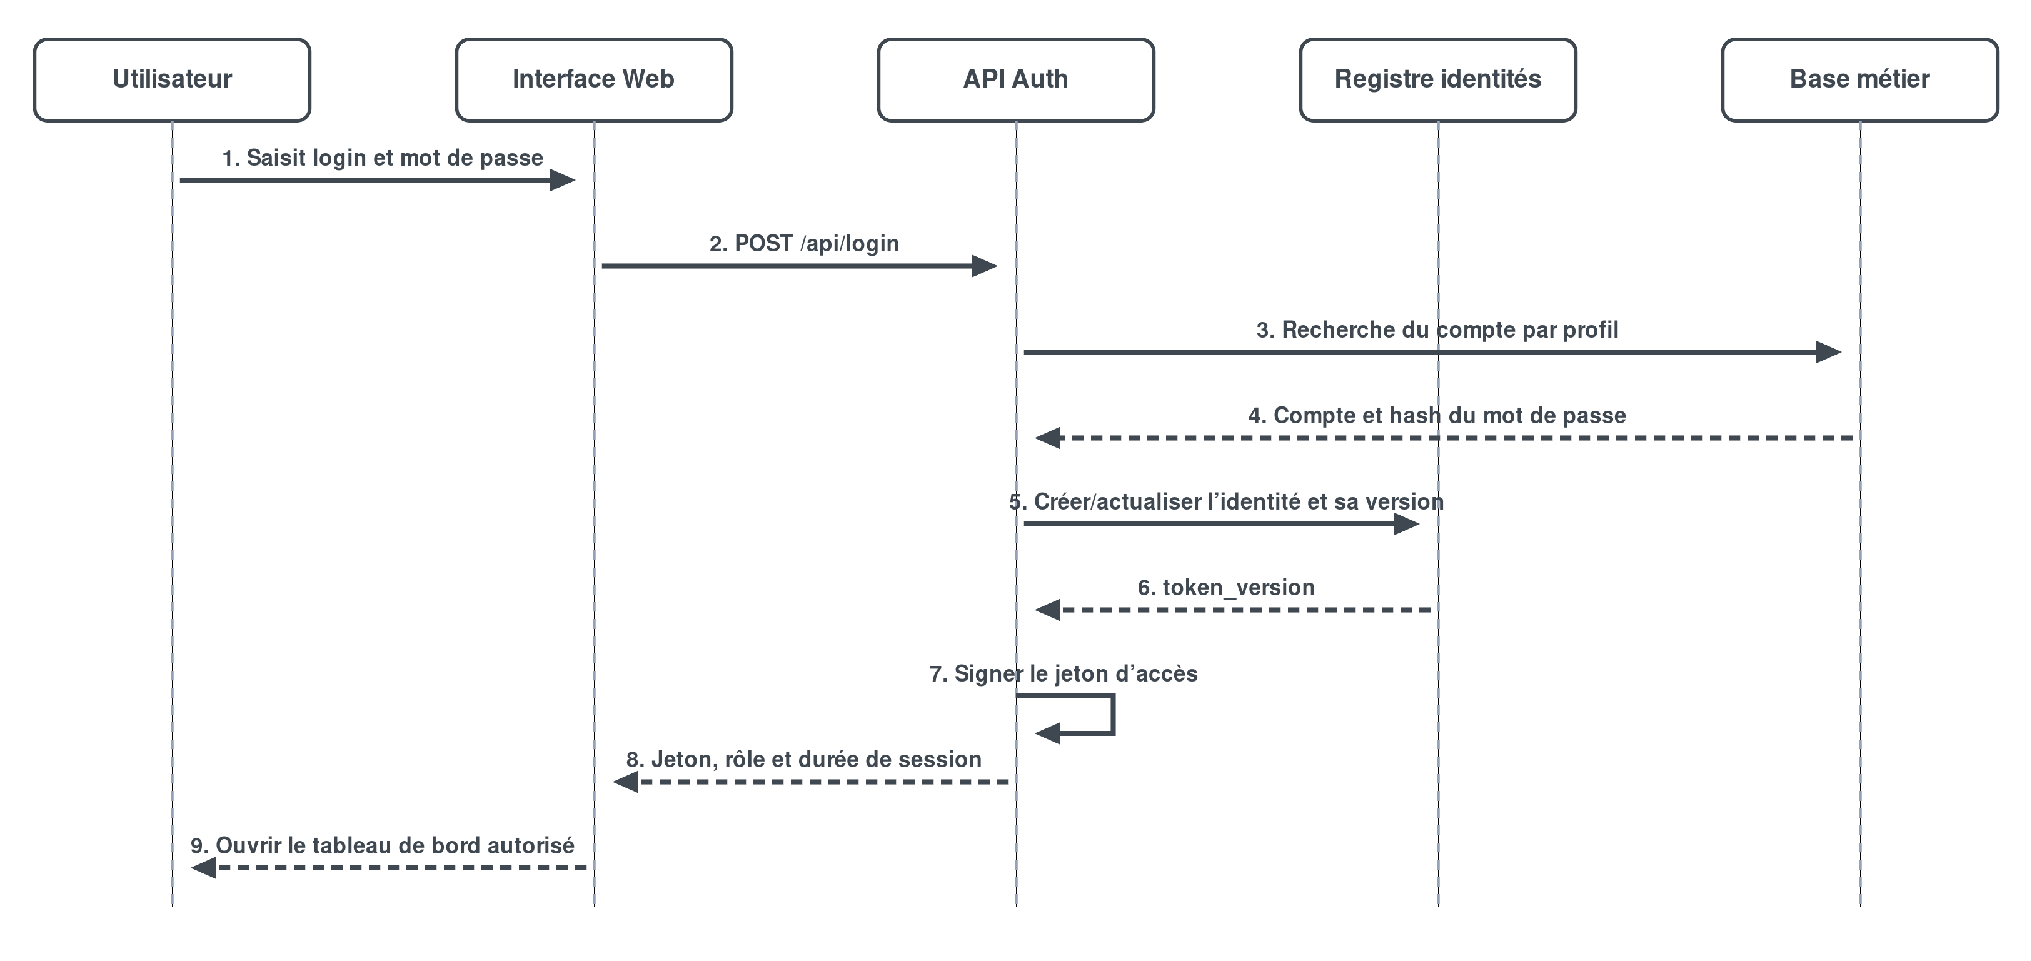
\includegraphics{figures/argos_05_sequence_authentification.pdf}%
}
\caption{Séquence d'authentification signée}
\label{fig-argos-seq-auth}
\tablesourcepromoteurs

\end{figure}

La sécurisation des accès et l'initialisation du parc logistique reposent sur des chaînes de transactions univoques qui garantissent l'intégrité de la plateforme. La séquence d'authentification formalise le processus d'accès par jetons signés : lors de la tentative de connexion d'un utilisateur, le système valide les informations d'identification au sein de la table de profils dédiée, synchronise le registre central des identités et génère un jeton sécurisé dont la validité est contrôlée à chaque requête par l'intermédiaire de la version de la clé (\texttt{token\_version}) et de l'état du compte.

\begin{figure}[htbp]
\centering
\resizebox{0.85\textwidth}{!}{%
  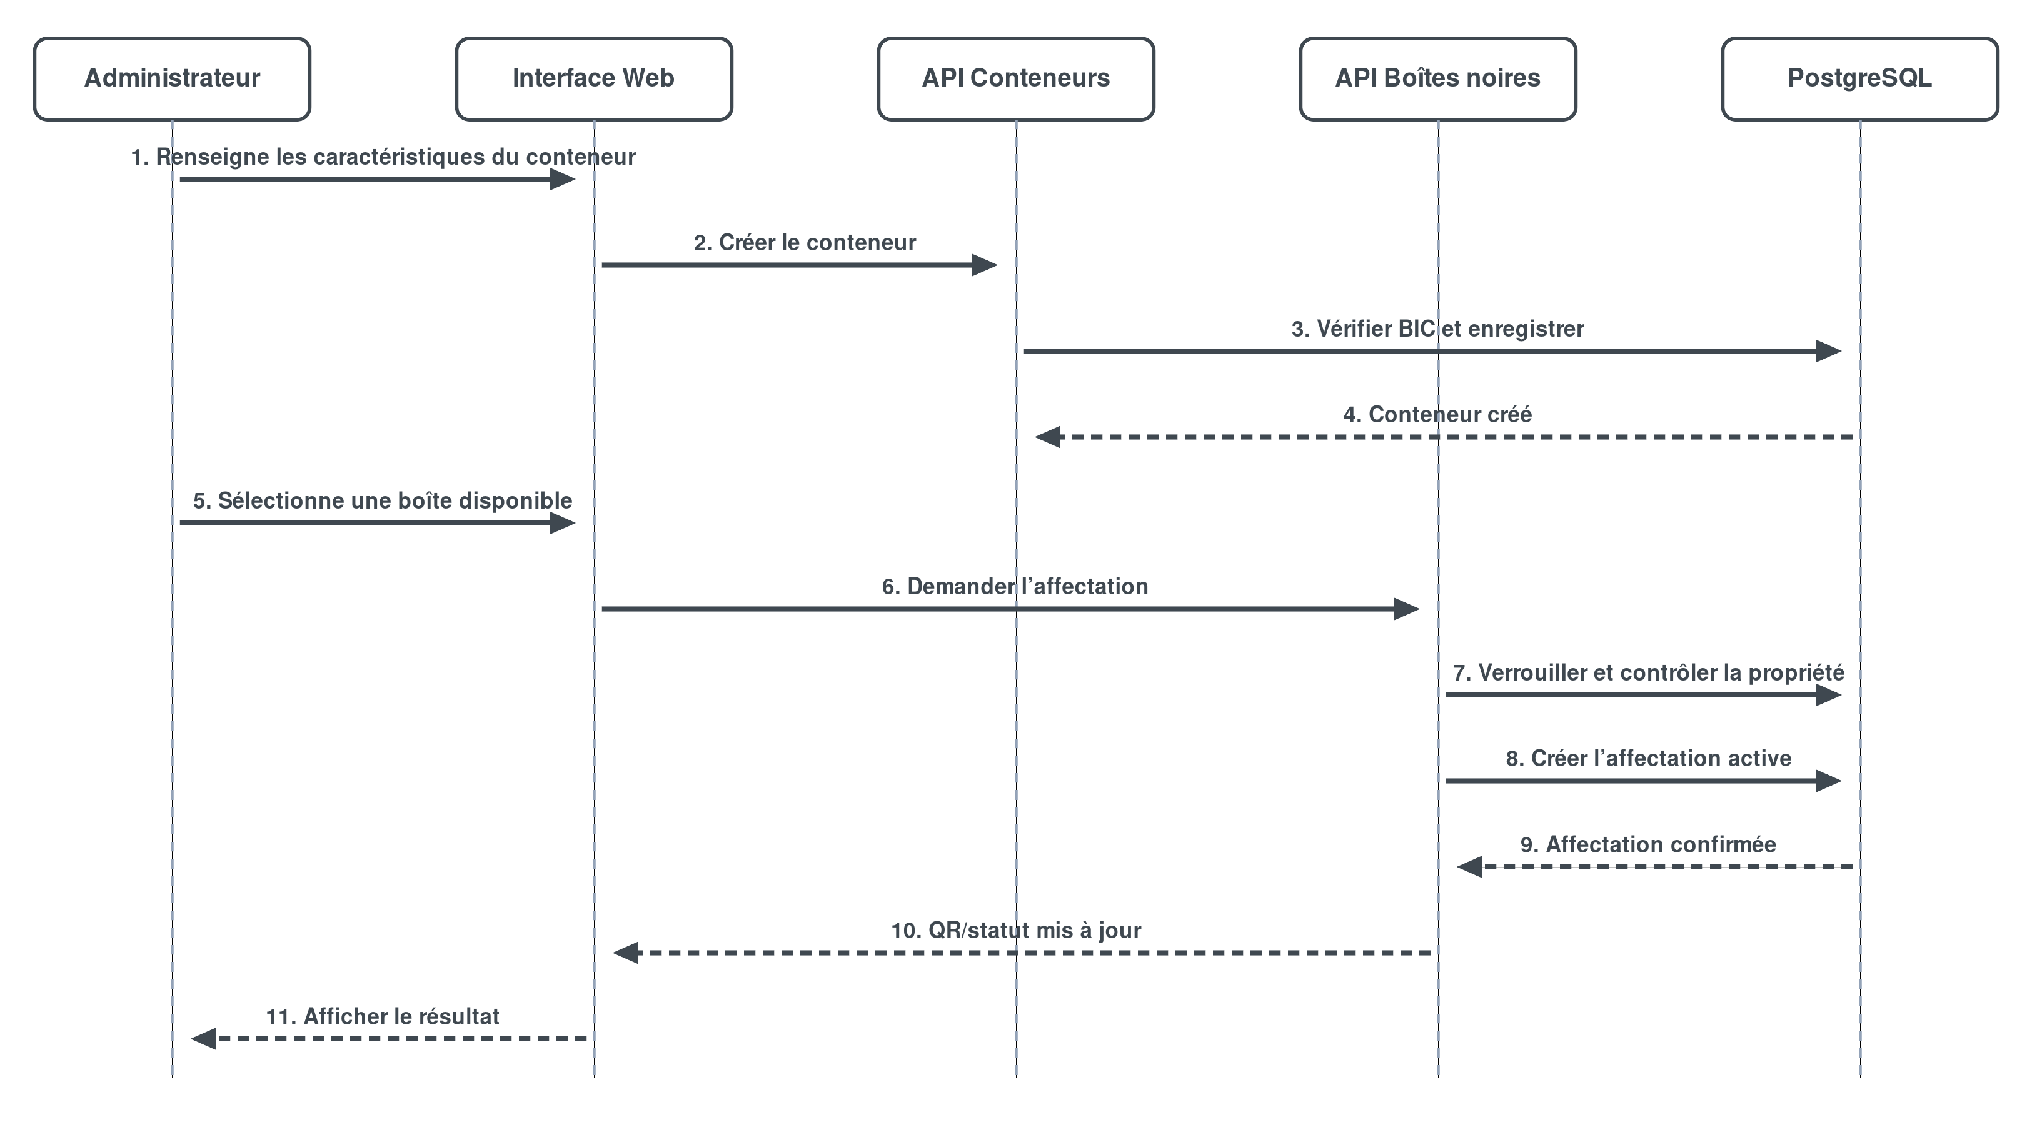
\includegraphics{figures/argos_06_sequence_gestion_conteneur_boite.pdf}%
}
\caption{Séquence de création et d'affectation conteneur--boîte}
\label{fig-argos-seq-affectation}
\tablesourcepromoteurs

\end{figure}

Le diagramme de gestion et d'affectation orchestre la création des unités logistiques. Le système réceptionne l'identifiant du conteneur, l'enrichit et le normalise dynamiquement via l'interopérabilité avec les services d'API externes (notamment l'API BIC), avant d'effectuer l'association transactionnelle avec un boîtier disponible dans le parc. Ce couplage garantit qu'aucune entité physique n'évolue sans rattachement traçable.


\subsubsection{Contrat et enrôlement IoT}

\begin{figure}[htbp]
\centering
\resizebox{0.85\textwidth}{!}{%
  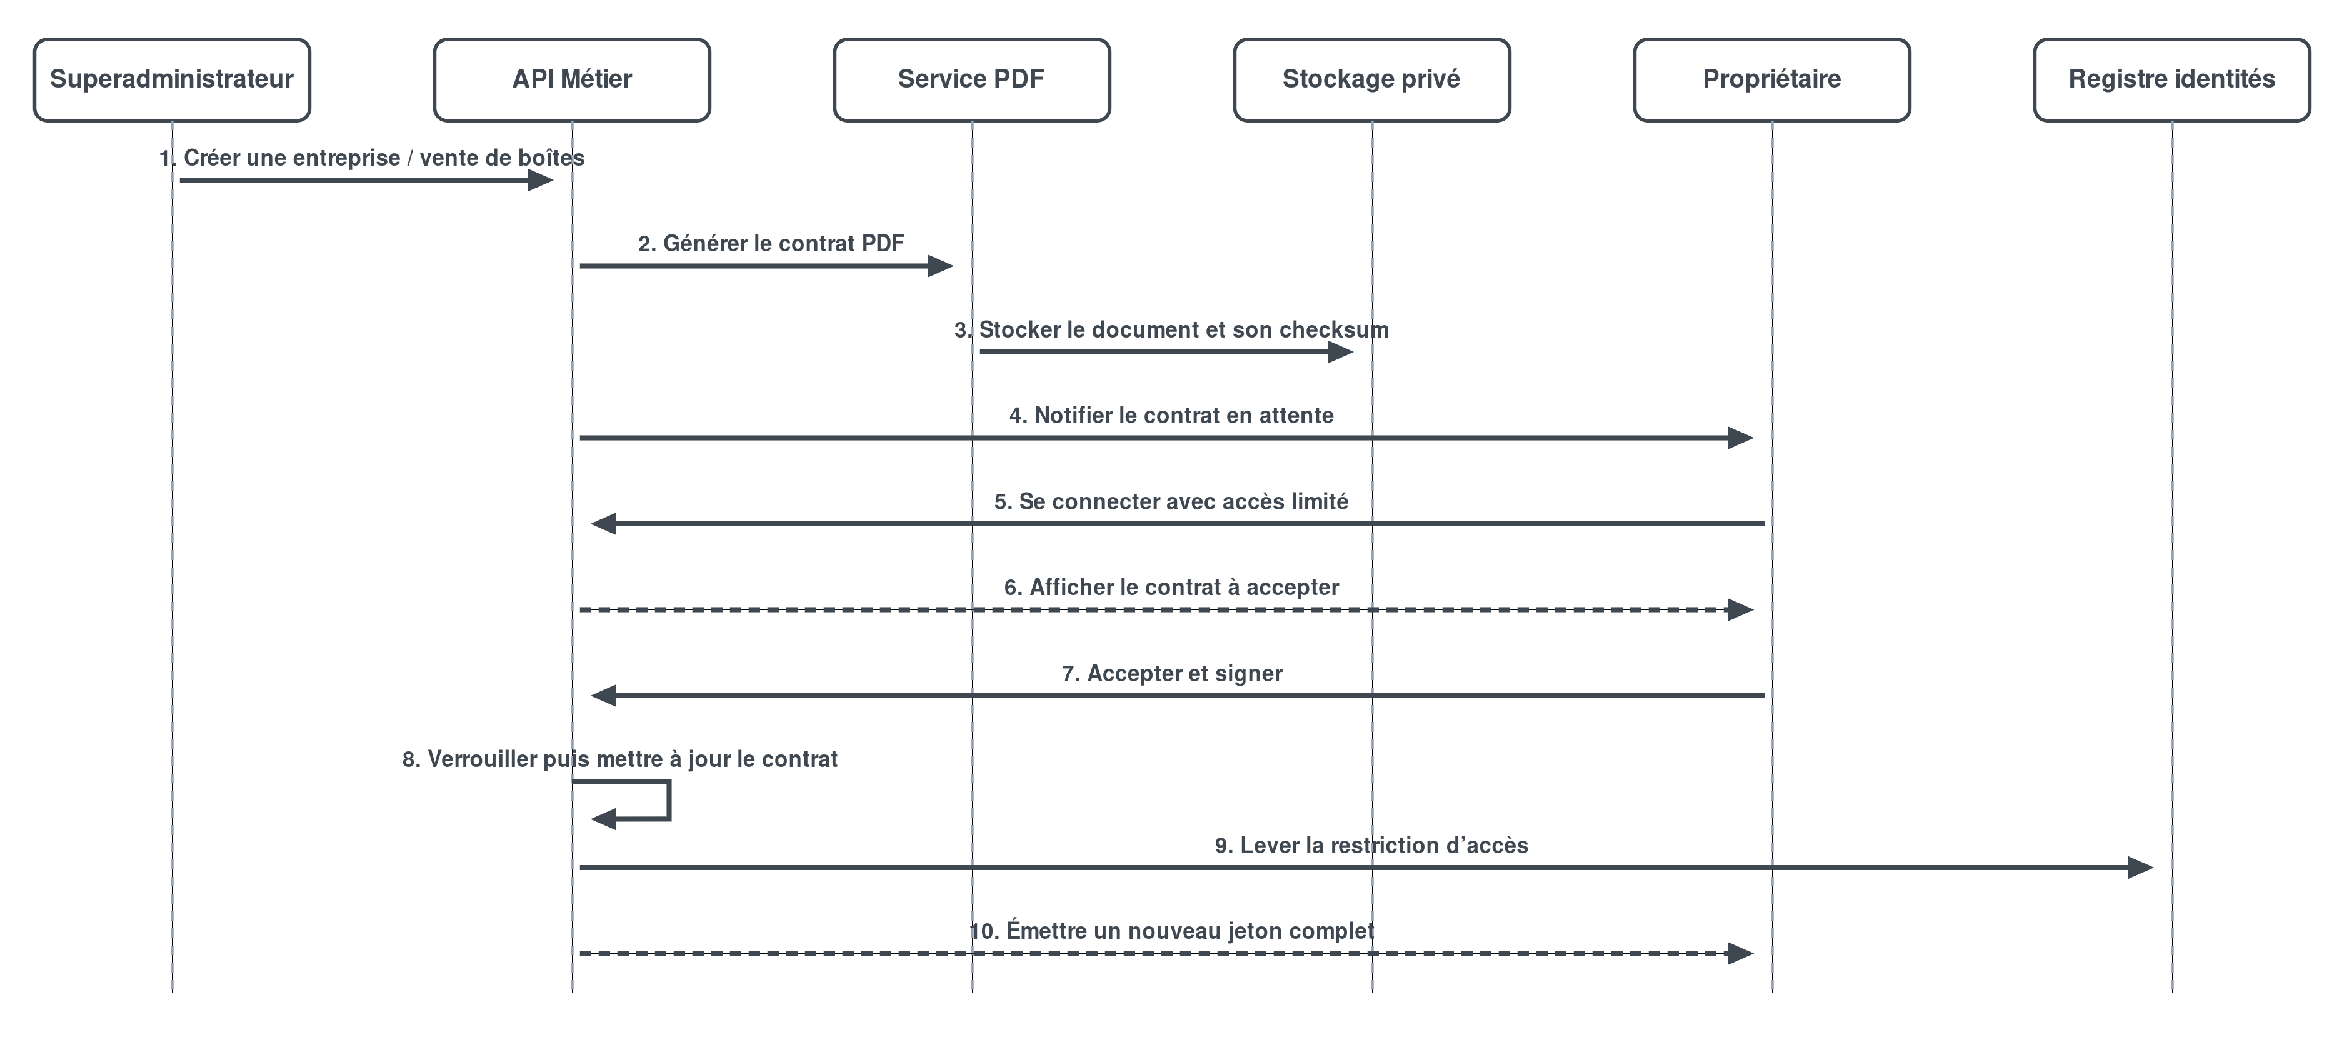
\includegraphics{figures/argos_07_sequence_contrat.pdf}%
}
\caption{Séquence de génération et d'acceptation d'un contrat}
\label{fig-argos-seq-contrat}
\tablesourcepromoteurs

\end{figure}

Le cycle de contractualisation et de provisionnement matériel matérialise la transition entre la gestion administrative et l'exploitation technique sur le terrain. Le diagramme de séquence des contrats retrace la chaîne décisionnelle allant de l'initiation de l'entreprise par le superadministrateur jusqu'à la signature numérique et l'archivage sécurisé du document dans le stockage privé. Cette validation lève automatiquement les restrictions d'accès initiales dans le registre d'identités et octroie au propriétaire ses pleines prérogatives opérationnelles.

\begin{figure}[htbp]
\centering
\resizebox{0.85\textwidth}{!}{%
  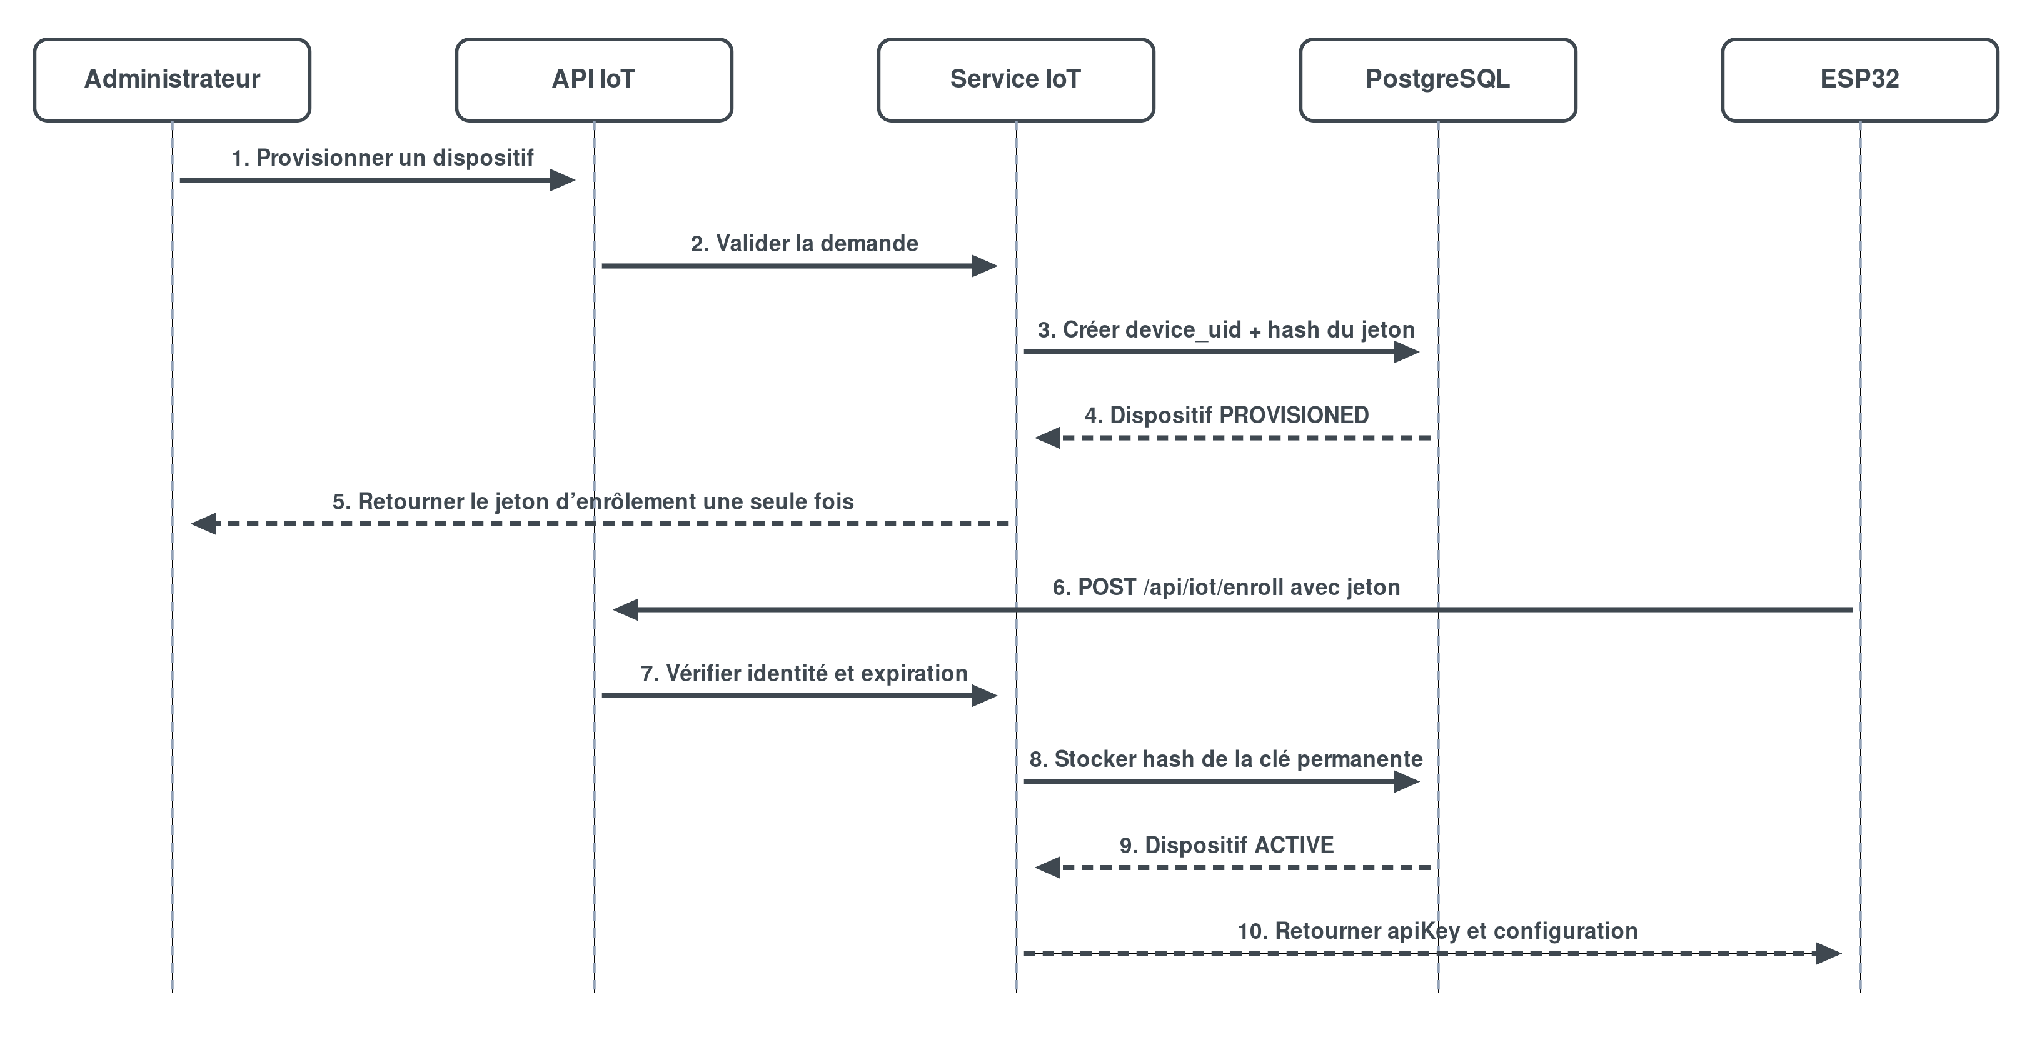
\includegraphics{figures/argos_08_sequence_enrolement_iot.pdf}%
}
\caption{Séquence de provisionnement et d'enrôlement d'un ESP32}
\label{fig-argos-seq-enrolement}
\tablesourcepromoteurs

\end{figure}

Dans la continuité, le processus d'enrôlement de l'ESP32 formalise le mécanisme d'initialisation sécurisée du dispositif embarqué. À partir d'un jeton temporaire valable par défaut 24 heures, le système authentifie le matériel, génère une empreinte, supprime le jeton initial après validation et délivre une clé permanente, faisant basculer l'état du boîtier à l'état \code{ACTIVE} au sein de la flotte.


\subsubsection{Télémétrie, commande, voyage et déstockage}

\begin{figure}[htbp]
\centering
\resizebox{0.85\textwidth}{!}{%
  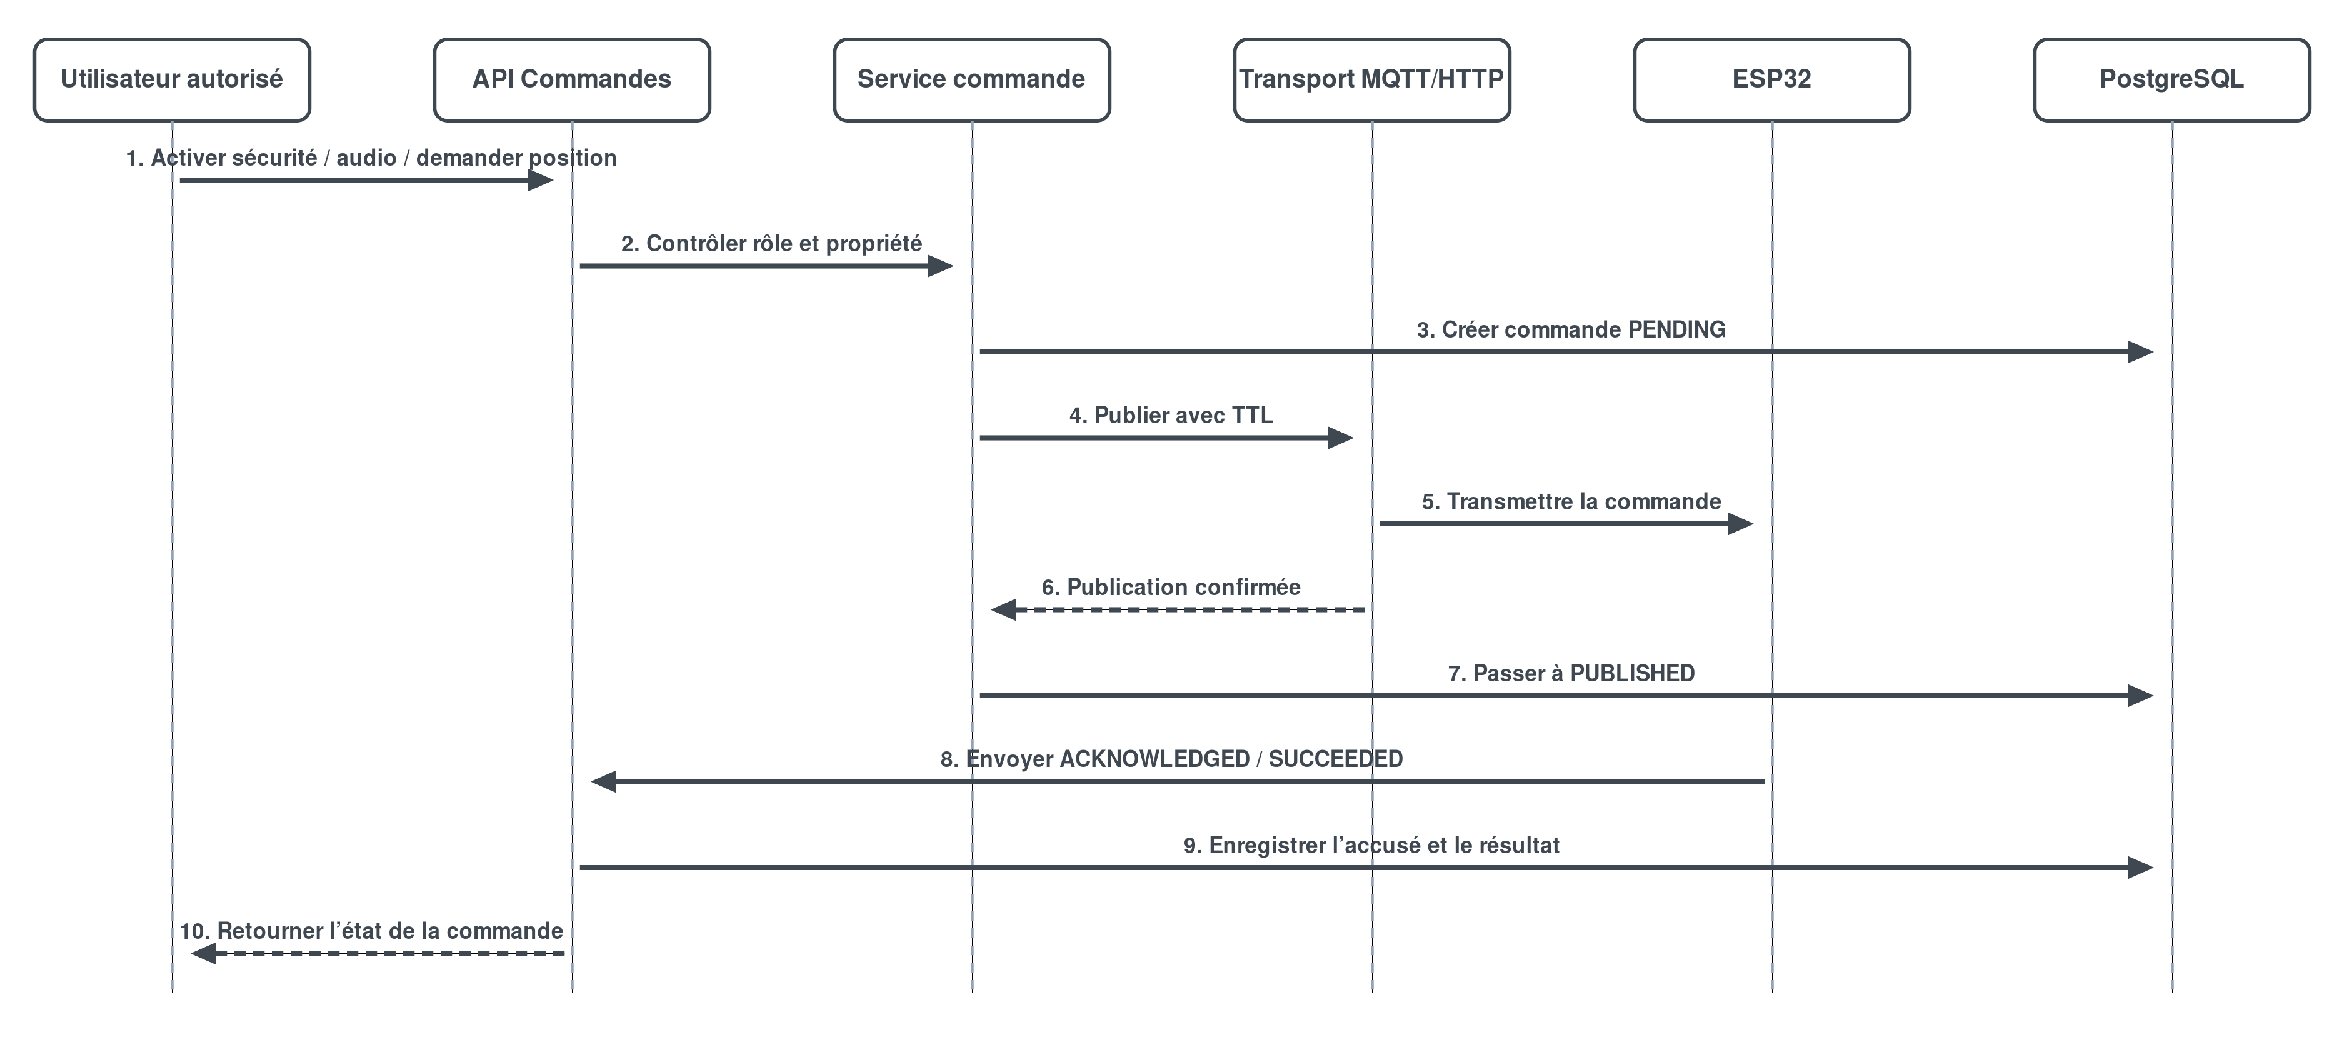
\includegraphics{figures/argos_10_sequence_commande_iot.pdf}%
}
\caption{Séquence d'émission et d'acquittement d'une commande}
\label{fig-argos-seq-commande}
\tablesourcepromoteurs

\end{figure}

L'exploitation quotidienne de la solution s'appuie sur des flux dynamiques complexes. Concernant le pilotage matériel, le diagramme d'émission de commandes illustre la boucle de transmission à distance vers les boîtiers. Les commandes transitent par des états stricts (\code{PENDING}, \code{PUBLISHED}, \code{ACKNOWLEDGED}, \code{SUCCEEDED}, \code{FAILED} ou \code{EXPIRED}), l'acquittement portant explicitement sur le \code{deviceUid} pour certifier l'exécutant.

\begin{figure}[htbp]
\centering
\resizebox{0.85\textwidth}{!}{%
  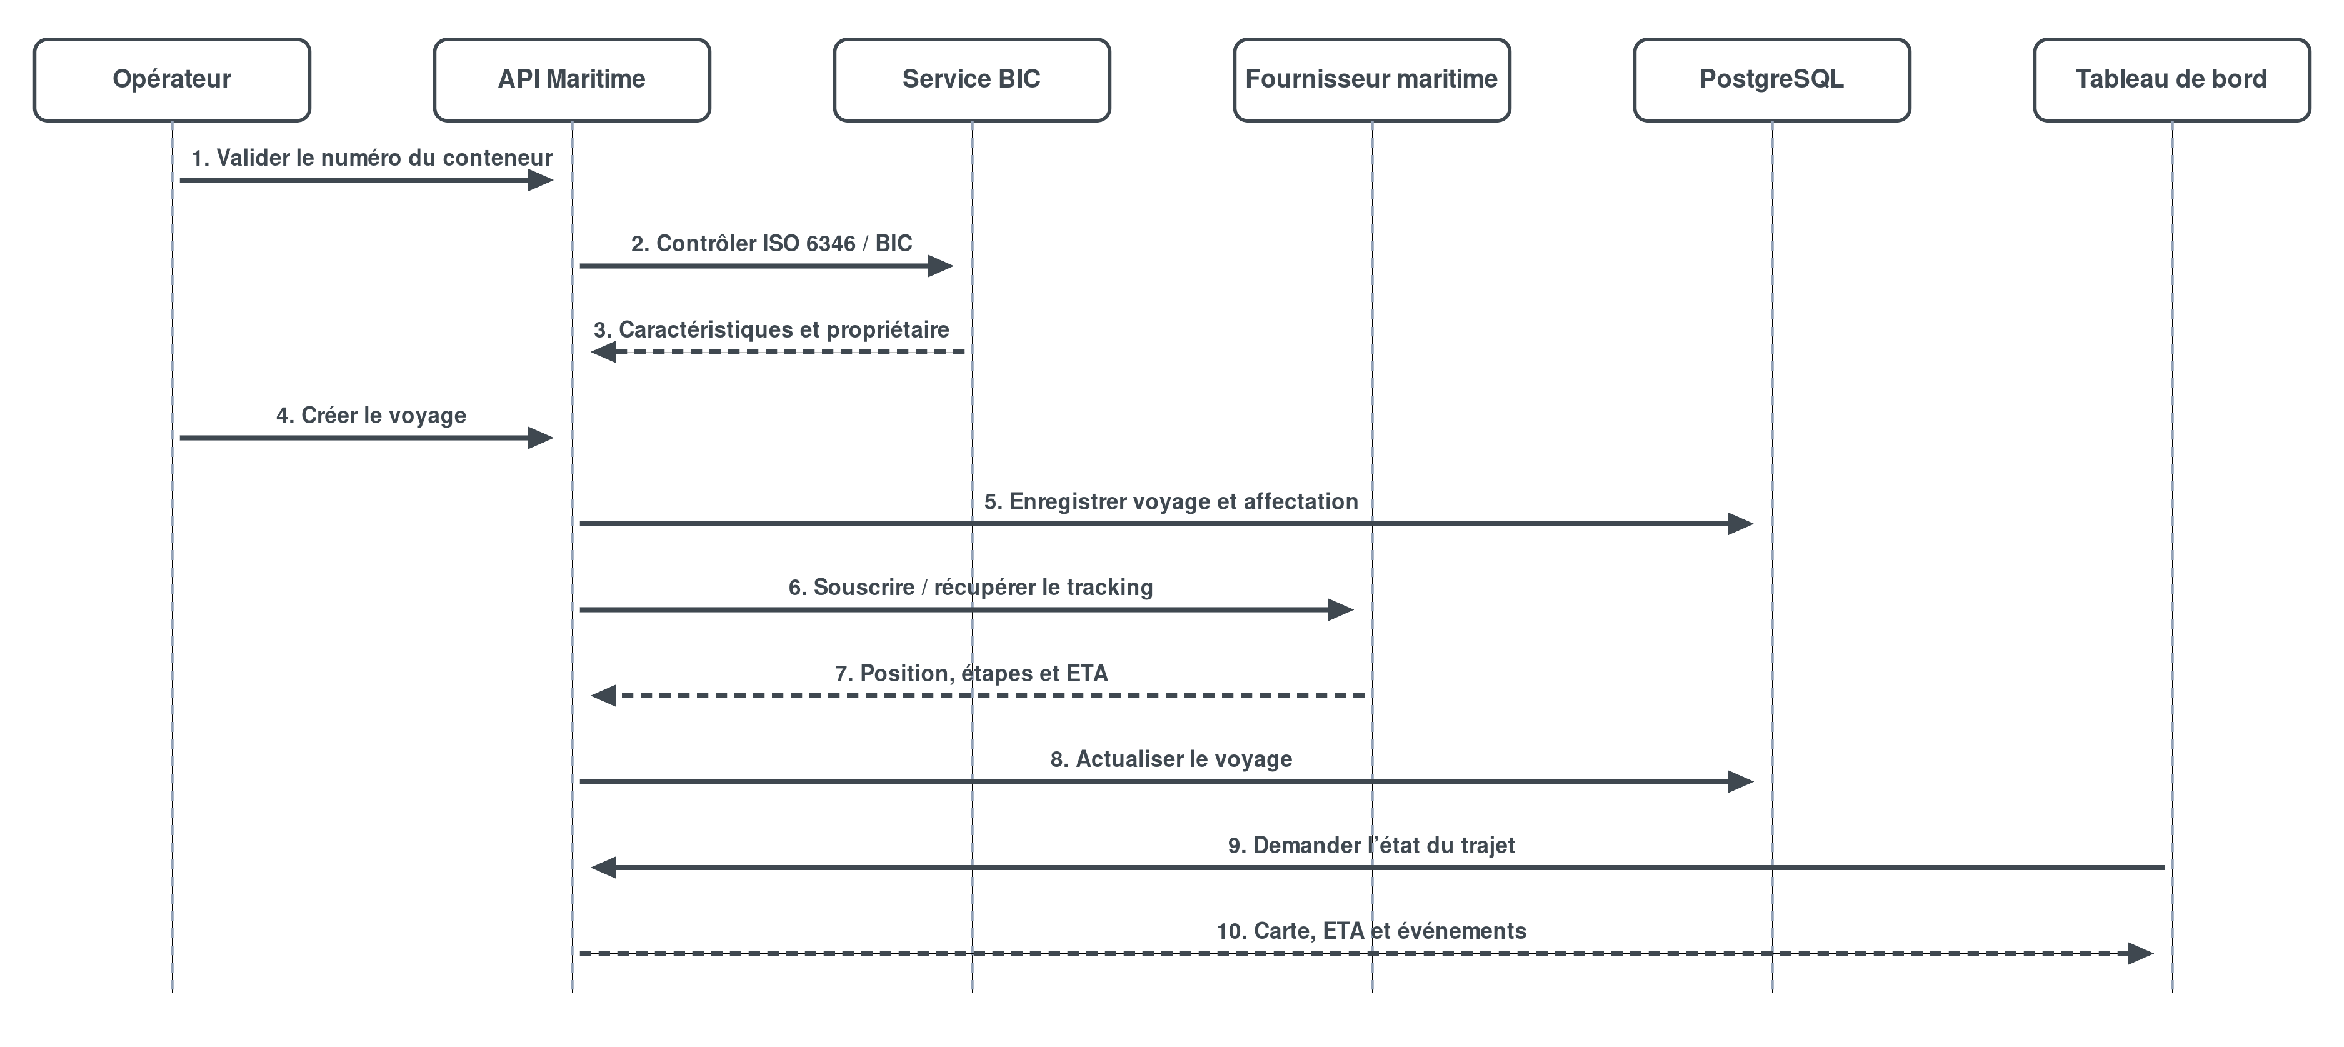
\includegraphics{figures/argos_11_sequence_voyage_tracking.pdf}%
}
\caption{Séquence de création et de suivi d'un voyage maritime}
\label{fig-argos-seq-voyage}
\tablesourcepromoteurs

\end{figure}

Le suivi des voyages maritimes met en évidence le rapprochement analytique entre la position GPS autonome du conteneur (transmise par la télémétrie IoT) et les données AIS du navire porteur. Cette corrélation permet d'anticiper les litiges, d'identifier le port le plus proche et de calculer précisément les distances de transport.

\begin{figure}[htbp]
\centering
\resizebox{0.85\textwidth}{!}{%
  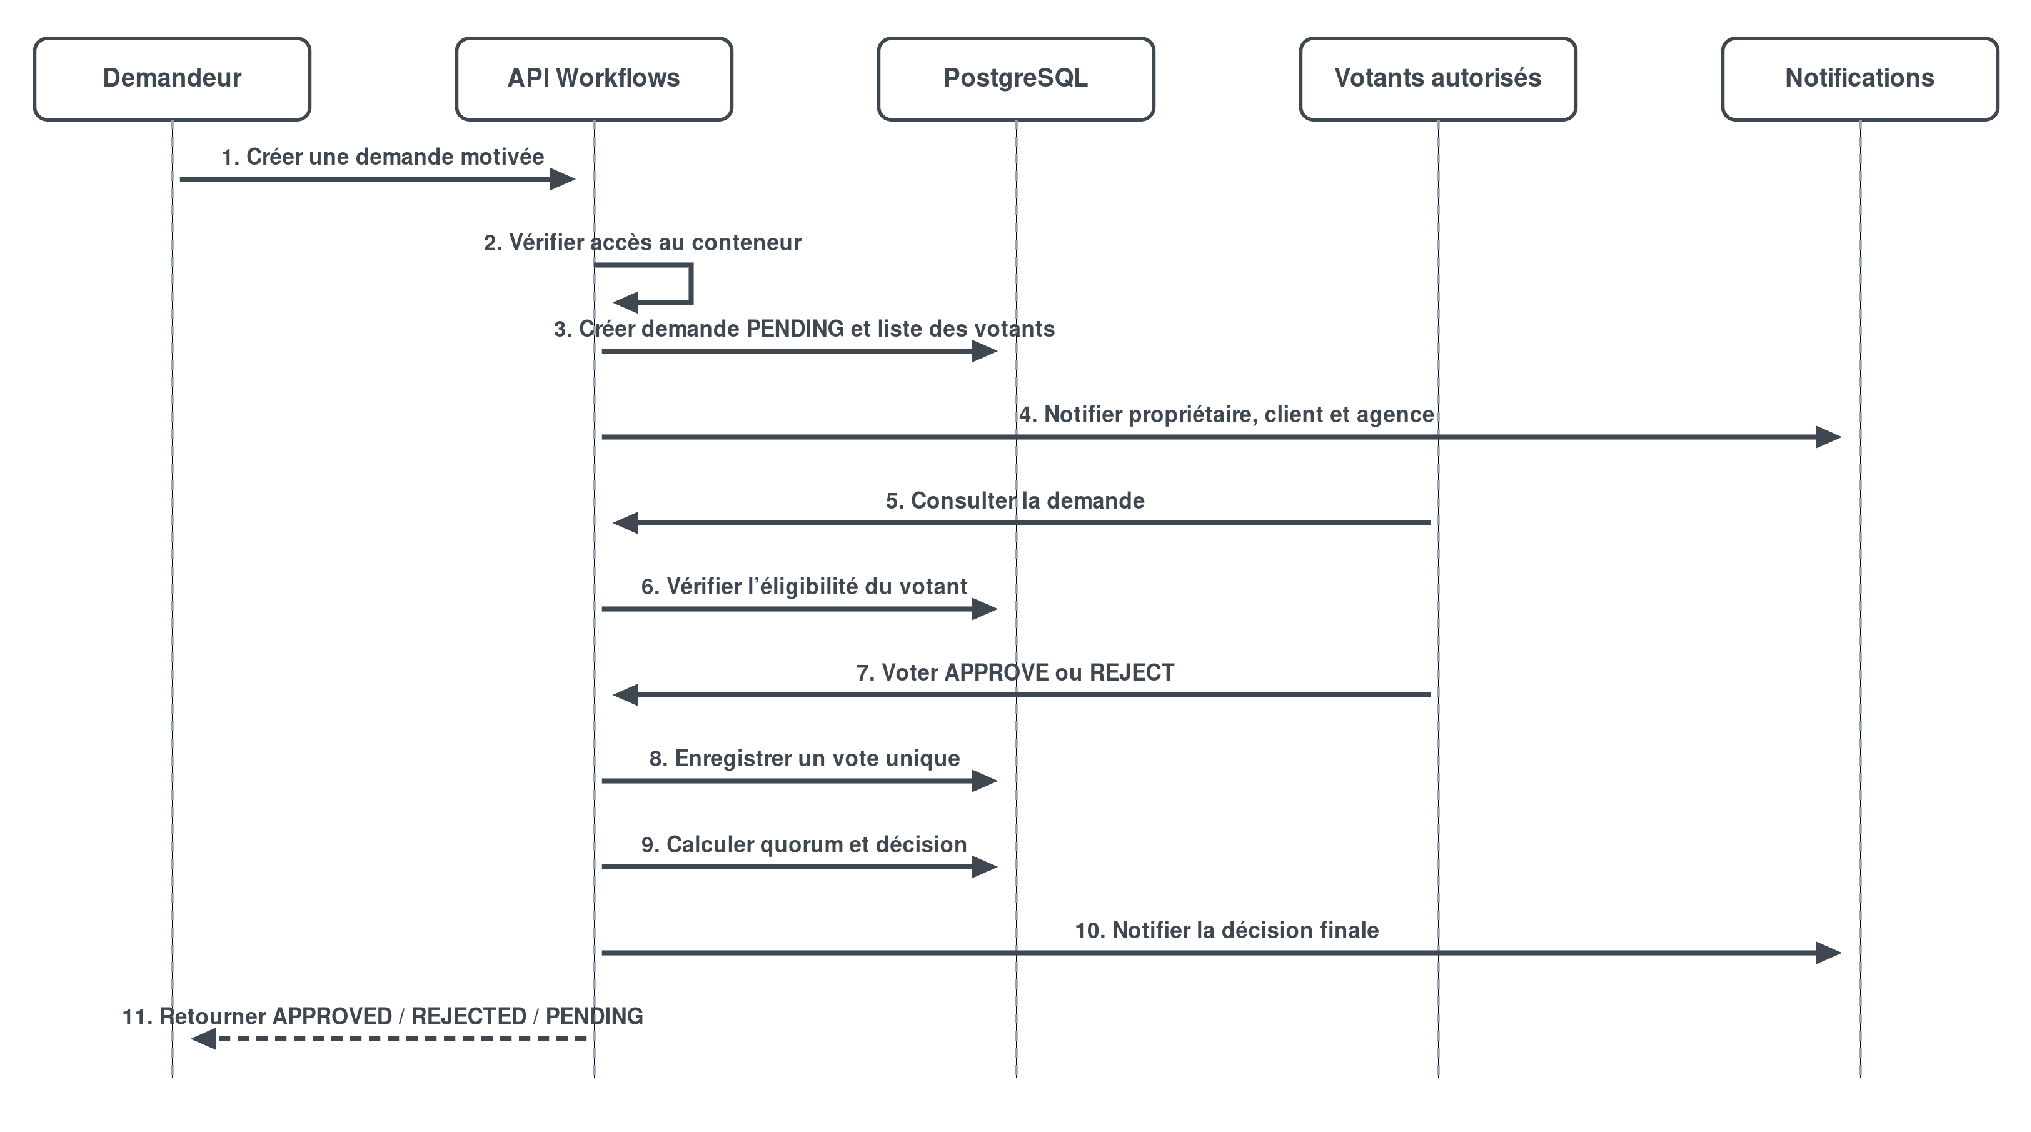
\includegraphics{figures/argos_12_sequence_destockage.pdf}%
}
\caption{Séquence de demande, vote et décision de déstockage}
\label{fig-argos-seq-destockage}
\tablesourcepromoteurs

\end{figure}

Enfin, le processus de déstockage formalise un workflow décisionnel collaboratif et sécurisé : l'émission d'une demande identifiant les votants et l'échéance déclenche une procédure d'approbation multipartite. À l'issue des votes requis, le worker automatisé génère le rapport final d'expertise, détache la boîte du conteneur et maintient temporairement l'accès selon le paramètre \code{visibility\_until}.

% \\\\\\\\\\\\\\\\\\\\\\\\\\\\\\\\\\\
\subsubsection{Chaîne de télémétrie de bout en bout}

\begin{figure}[htbp]
\centering
\resizebox{0.95\textwidth}{!}{%
  \resizebox{!}{0.82\textheight}{%
\begin{tikzpicture}[
  font=\sffamily\small,
  lane/.style={draw=argosrule,rounded corners=3pt,fill=argospale,
    minimum width=4.2cm,minimum height=1.15cm,align=center},
  procstep/.style={draw=argosmid,rounded corners=3pt,fill=white,
    minimum width=4.6cm,minimum height=1.15cm,align=center,line width=.8pt},
  store/.style={draw=argosnavy,cylinder,shape border rotate=90,aspect=.24,
    fill=argoslight,minimum width=4.3cm,minimum height=1.45cm,align=center,line width=.9pt},
  decision/.style={draw=argosnavy,diamond,aspect=2.25,fill=argospale,
    minimum width=4.5cm,minimum height=1.5cm,align=center,line width=.9pt},
  flow/.style={draw=argosgray,line width=.85pt,-{Stealth[length=2.4mm]}},
  async/.style={draw=argosmid,dashed,line width=.85pt,-{Stealth[length=2.4mm]}},
  note/.style={font=\sffamily\scriptsize,align=center,text=argosgray}
]
\node[lane] (sta) at (-9.6,7.4) {ESP32 en mode station\\POST \texttt{/api/iot/telemetry}\\clé \texttt{X-Device-Key}};
\node[lane] (ap) at (0,7.4) {ESP32 en point d'accès\\GET local \texttt{/api/v1/telemetry}\\toutes les 1 à 30 s (2 s par défaut)};
\node[lane] (browser) at (9.6,7.4) {Navigateur ARGOS authentifié\\vérification de l'UID, affichage immédiat\\et file FIFO locale bornée};
\node[procstep] (route) at (0,5.1) {Route commune d'ingestion\\standard ou \texttt{direct-telemetry}};
\node[procstep] (validate) at (0,3.1) {Valider UUID, \texttt{deviceUid}, boîte,\\conteneur, horodatage, séquence et plages};
\node[decision] (identity) at (0,.8) {Identité, affectation\\et séquence valides ?};
\node[store] (rawreject) at (-8.0,-1.7) {PostgreSQL (voie standard)\\message brut rejeté\\et motif};
\node[procstep] (normalise) at (0,-1.7) {Normaliser la qualité capteur\\et remplacer GPS 0,0 par un\\repli navigateur déjà autorisé};
\node[procstep] (threshold) at (-7.6,-4.4) {Comparer aux seuils\\et construire les alertes};
\node[store] (redis) at (0,-4.4) {Redis\\clé latest (TTL 24 h)\\+ stream borné à 10 000};
\node[store] (postgres) at (7.6,-4.4) {PostgreSQL\\raw, lectures, positions, événements,\\notifications et audit (transaction)};
\node[procstep] (liveapi) at (-5.1,-7.1) {\texttt{/api/stats/live}\\Redis d'abord, PostgreSQL en repli};
\node[procstep] (ui) at (0,-9.1) {Partager la mesure dans l'application\\carte, boîtes, statistiques, alertes, événements};
\node[procstep] (notify) at (7.0,-7.1) {Notifier les parties liées\\application et courriel, avec anti-doublon};

\draw[flow] (sta.south) -- (route.north west);
\draw[flow] (ap.east) -- (browser.west);
\draw[flow] (browser.south) |- node[note,pos=.25,right]{POST Bearer} (route.east);
\draw[flow] (route) -- (validate);
\draw[flow] (validate) -- (identity);
\draw[flow] (identity.west) -- node[note,above]{non} (rawreject.east);
\draw[flow] (identity) -- node[note,right]{oui} (normalise);
\draw[flow] (normalise.west) to[out=200,in=70] (threshold.north);
\draw[flow] (threshold.east) -- (redis.west);
\draw[flow] (redis.east) -- (postgres.west);
\draw[flow] (redis) -- (liveapi);
\draw[flow] (liveapi) -- (ui.north west);
\draw[flow] (browser.south east) |- node[note,pos=.24,right]{rendu local avant synchronisation} (ui.east);
\draw[async] (postgres) -- (notify);
\draw[async] (notify.south) |- (ui.east);
\end{tikzpicture}%
}
%
}
\caption{Chaîne de télémétrie de bout en bout}
\label{fig-argos-flux-telemetrie}
\tablesourcepromoteurs

\end{figure}

\subsubsection{Fichiers JSON de télémétrie}

\begingroup
\small
\begin{longtable}{@{}p{4.7cm}p{2.5cm}p{6.8cm}@{}}
\caption{Champs du message de télémétrie et règles de validation}
\label{tab-contrat-telemetrie}\\
\tableheadrow \thc{Chemin JSON} & \thc{Type} & \thc{Règle et utilisation} \\
\midrule
\endfirsthead
\tableheadrow \thc{Chemin JSON} & \thc{Type} & \thc{Règle et utilisation} \\
\midrule
\endhead
\code{messageId} & UUID & Identifiant de message unique ; doublon traité de manière idempotente \\
\hline
\code{type} & chaîne & Valeur obligatoire \code{telemetry} \\
\hline
\code{deviceUid} & chaîne & Identité unique du matériel, comparée à \code{iot\_devices.device\_uid} \\
\hline
\code{blackBoxId} & entier positif & Doit correspondre à l'association active du dispositif \\
\hline
\code{containerId} & chaîne ou nul & Normalisé en majuscules et contrôlé si une affectation existe \\
\hline
\code{timestamp} & ISO-8601 & Fuseau accepté ; écart maximal de six heures avec le serveur \\
\hline
\code{sequence} & entier $\geq 0$ & Doit être strictement supérieur à la dernière séquence traitée \\
\hline
\code{position.latitude} & réel & Intervalle $[-90,90]$ \\
\hline
\code{position.longitude} & réel & Intervalle $[-180,180]$ \\
\hline
\code{position.accuracy} & réel & Intervalle $[0,100000]$ mètres \\
\hline
\code{position.speed} & réel & Intervalle $[0,1000]$ ; affiché et comparé au seuil \\
\hline
\code{position.heading} & réel & Intervalle $[0,360]$ degrés \\
\hline
\code{position.source} & chaîne & \code{ESP32}, \code{DIRECT\_WIFI} ou \code{BROWSER\_FALLBACK} \\
\hline
\code{sensors.temperature} & réel & $[-80,120]$ \textdegree C ; neutralisé si DHT invalide \\
\hline
\code{sensors.humidity} & réel & $[0,100]$ \% ; neutralisé si DHT invalide \\
\hline
\code{sensors.shock} & réel & $[0,200]$ g ; neutralisé si MPU invalide \\
\hline
\code{sensors.pressure} & réel & $[300,1200]$ hPa ; neutralisé si non mesuré \\
\hline
\code{sensors.flameDetected} & booléen & Déclenche une alerte si vrai \\
\hline
\code{sensors.doorOpen} & booléen & Déclenche une alerte lorsque la sécurité est active \\
\hline
\code{sensors.batteryLevel} & réel & $[0,100]$ \% ; neutralisé si valeur non mesurée \\
\hline
\code{sensors.lightLevel} & réel & Valeur optionnelle $[0,4095]$ \\
\hline
\code{sensors.soundLevel} & réel & Valeur optionnelle $[0,4095]$ \\
\hline
\code{sensors.distanceCm} & réel & Valeur optionnelle $[0,1000]$ cm \\
\hline
\nolinkurl{sensors.accelerationX/Y/Z} & réels & Valeurs optionnelles dans $[-200,200]$ \\
\hline
\code{sensors.securityAlarm} & booléen & État synthétique de l'alarme locale \\
\hline
\code{modes.securityEnabled} & booléen & Sécurité des portes activée ou bloquée \\
\hline
\nolinkurl{modes.audioRecordingEnabled} & booléen & État de l'enregistrement audio \\
\hline
\nolinkurl{modes.audioListeningEnabled} & booléen & État de l'écoute audio \\
\hline
\nolinkurl{modes.flameDetectionEnabled} & booléen & État de la détection de flamme \\
\hline
\code{quality.dhtValid} & booléen & Fiabilité température/humidité \\
\hline
\code{quality.mpuValid} & booléen & Fiabilité choc/accélérations \\
\hline
\code{quality.gpsValid} & booléen & Validité du GPS embarqué \\
\hline
\code{quality.distanceValid} & booléen & Validité de la distance ultrasonique \\
\hline
\code{quality.sdReady} & booléen & Disponibilité de la carte SD \\
\hline
\code{quality.pressureMeasured} & booléen & Distingue une mesure réelle d'une valeur de substitution \\
\hline
\code{quality.batteryMeasured} & booléen & Distingue une mesure réelle d'une estimation \\
\hline
\code{quality.timestampSource} & chaîne & Origine de l'heure, appareil ou navigateur/API \\
\tablebottomrule
\end{longtable}
\tablesourcepromoteurs
\endgroup

\subsubsection{Ordre de traitement}

Après validation et contrôle de l'association, l'application applique le
repli de position et transforme en \code{NULL} les capteurs déclarés
invalides. Elle publie ensuite le document normalisé dans Redis DB1. La même
requête insère les vues durables dans PostgreSQL et valide la transaction.
L'ordre logique est donc :
\[
\text{route de télémétrie}
\rightarrow \text{validation}
\rightarrow \text{Redis temps réel}
\rightarrow \text{PostgreSQL durable}.
\]

Le message brut est préparé dans la transaction PostgreSQL pour conserver le
JSON reçu. La voie distante tente également de journaliser les messages
rejetés ; la voie directe annule actuellement sa transaction en cas de rejet.

\subsubsection{Propagation de l'identité et de la séquence}

\begin{table}[htbp]
\centering
\caption{Traçabilité de l'UID et de la séquence dans chaque représentation}
\label{tab-tracabilite-uid-sequence}
\begin{tabularx}{\textwidth}{@{}p{3.6cm}p{5.0cm}X@{}}
\tableheadrow \thc{Destination} & \thc{Identité} & \thc{Séquence et lien} \\
\midrule
Redis latest/stream & \code{deviceUid} direct & \code{sequence} directe et \code{messageId} \\
\hline
\code{iot\_raw\_messages} & \code{device\_uid} direct & \code{message\_id} pointe vers le JSON contenant la séquence \\
\hline
\code{sensor\_readings} & \code{device\_id} vers \code{iot\_devices} & \code{sequence} directe et \code{raw\_message\_id} \\
\hline
\code{positions} & \code{device\_id} vers \code{iot\_devices} & Lien \code{raw\_message\_id} vers le message et sa séquence \\
\hline
\code{evenement\_save} & \code{device\_uid} direct & \code{sequence} directe, boîte et horodatage \\
\hline
\code{notifications} & \code{device\_uid} direct pour les alertes IoT & \code{sequence} directe et boîte concernée \\
\hline
\code{audit\_logs} & UID dans \code{entity\_id} & Séquence et UUID dans \code{details} JSONB \\
\tablebottomrule
\end{tabularx}
\tablesourcepromoteurs
\end{table}

Cette propagation permet de trier les mesures par dispositif, détecter un
trou ou un rejeu de séquence, et relier une alerte à la mesure qui l'a
produite, même lorsque la table concernée ne duplique pas physiquement les
deux colonnes.

\subsubsection{Partage distant et QR code}

À l'ouverture d'une session directe unique, ARGOS crée une notification avec
le lien distant et évite une nouvelle annonce pendant 30 minutes pour le
même acteur. Si la boîte est liée à un conteneur, le propriétaire, les agences
actives et les clients abonnés ayant une adresse valide reçoivent le lien et
le QR code par courriel. Le scan n'annule pas les restrictions : une
authentification ARGOS et un lien actif avec la ressource restent obligatoires.
Pour une boîte non affectée, l'information demeure dans le périmètre du
superadministrateur.

\subsubsection{Sécurité des portes et diffusion des alertes}

\begin{figure}[htbp]
\centering
\resizebox{0.95\textwidth}{!}{%
  % Activation/désactivation du mode sécurité, avec variantes directe et distante.
\resizebox{\textwidth}{!}{%
\begin{tikzpicture}[
  font=\sffamily\small,
  participant/.style={draw=argosnavy,rounded corners=2pt,fill=argoslight,
    minimum width=3.6cm,minimum height=1.1cm,align=center,line width=.9pt,font=\sffamily\small\bfseries},
  life/.style={draw=argosrule,dashed,line width=.8pt},
  call/.style={draw=argosgray,line width=.9pt,-{Stealth[length=2.5mm]}},
  reply/.style={draw=argosgray,dashed,line width=.85pt,-{Stealth[length=2.5mm]}},
  async/.style={draw=argosmid,dashed,line width=.9pt,-{Stealth[length=2.5mm]}},
  note/.style={draw=argosrule,rounded corners=3pt,fill=argospale,
    align=left,inner sep=5pt,font=\sffamily\small},
  msg/.style={font=\sffamily\small,fill=white,inner sep=1.8pt,align=center}
]

% -----------------------------------------------------------------
% PARTICIPANTS
% -----------------------------------------------------------------
\node[participant] (manager) at (-14.0,7.8) {Gestionnaire\\autorisé};
\node[participant] (browser) at (-9.2,7.8) {Interface web\\ARGOS};
\node[participant] (esp) at (-4.5,7.8) {ESP32-S3\\local ou distant};
\node[participant] (api) at (0.2,7.8) {Route sécurité\\Flask};
\node[participant] (command) at (5.0,7.8) {Service de\\commandes};
\node[participant] (pg) at (9.8,7.8) {PostgreSQL +\\journal chaîné};
\node[participant] (parties) at (14.6,7.8) {Parties liées\\application / e-mail};

\foreach \p in {manager,browser,esp,api,command,pg,parties}
  \draw[life] (\p.south) -- ++(0,-17.0);

% -----------------------------------------------------------------
% FLUX PRINCIPAL & DÉBUT SESSION
% -----------------------------------------------------------------
\draw[call] (-14.0,6.45) -- node[msg,above]{1. basculer « Mode sécurité des portes »} (-9.2,6.45);

\node[note,anchor=west,text width=7.2cm] at (-8.8,5.25)
  {2. Vérifier la session et le rôle : \texttt{superadmin}, \texttt{owner} ou \texttt{company}. La route contrôle ensuite que la boîte appartient au périmètre du gestionnaire.};

% -----------------------------------------------------------------
% VARIANTE A — WI-FI DIRECT
% -----------------------------------------------------------------
\node[note,anchor=west,text width=5.6cm] at (-13.9,3.65)
  {\textbf{Variante A} — session Wi-Fi directe active};

\draw[call] (-9.2,2.75) -- node[msg,above]{3A. POST local \texttt{/api/v1/security} \{enabled\}} (-4.5,2.75);
\draw[reply] (-4.5,2.05) -- node[msg,above]{mode appliqué et mémorisé} (-9.2,2.05);
\draw[call] (-9.2,1.25) -- node[msg,above]{4A. POST audit, \texttt{delivery=direct}, position autorisée} (0.2,1.25);

% -----------------------------------------------------------------
% VARIANTE B — COMMANDE DISTANTE
% -----------------------------------------------------------------
\node[note,anchor=west,text width=5.6cm] at (-13.9,-0.2)
  {\textbf{Variante B} — commande distante};

\draw[call] (-9.2,-1.1) -- node[msg,above]{3B. POST \texttt{/commands/security} \{enabled\}} (0.2,-1.1);
\draw[call] (0.2,-1.9) -- node[msg,above]{4B. créer \texttt{SET\_SECURITY\_MODE}} (5.0,-1.9);
\draw[call] (5.0,-2.7) -- node[msg,above]{\texttt{PENDING}, publication, puis \texttt{PUBLISHED}} (9.8,-2.7);

\draw[call] (0.2,-3.65) -- node[msg,above,align=center]{5. immédiatement : insérer événement et notification\\UID, auteur, rôle/poste, date, heure et position éventuelle} (9.8,-3.65);
\draw[reply] (9.8,-4.45) -- node[msg,above]{\texttt{COMMIT} durable} (0.2,-4.45);

\draw[async] (0.2,-5.25) -- node[msg,above]{6. sceller séparément \texttt{SECURITY\_MODE\_CHANGED}} (9.8,-5.25);
\draw[async] (9.8,-6.05) -- node[msg,above]{7. notification interne ; e-mail si conteneur et adresses liés} (14.6,-6.05);

\draw[reply] (0.2,-6.85) -- node[msg,above]{202 + message et horodatage} (-9.2,-6.85);
\draw[reply] (-9.2,-7.65) -- node[msg,above]{état affiché et événement visible} (-14.0,-7.65);

% -----------------------------------------------------------------
% EXECUTION DIFFÉRÉE ESP32
% -----------------------------------------------------------------
\draw[async] (5.0,-8.45) -- node[msg,above]{8. plus tard : transport ou interrogation de l'API} (-4.5,-8.45);
\draw[call] (-4.5,-9.25) -- node[msg,above]{accusé \texttt{SUCCEEDED} ou \texttt{FAILED}} (5.0,-9.25);
\draw[call] (5.0,-10.05) -- node[msg,above]{9. mettre à jour la commande et ses horodatages} (9.8,-10.05);

% -----------------------------------------------------------------
% NOTE FINALE
% -----------------------------------------------------------------
\node[note,anchor=north,text width=14.5cm] at (0.2,-10.9)
  {En mode direct, si ARGOS distant est momentanément inaccessible, l'action locale est immédiate mais son audit reste dans la FIFO du navigateur et ne peut être rejoué que par le même compte. En mode distant, l'événement atteste immédiatement la demande du gestionnaire ; l'accusé matériel arrive ensuite et met à jour la commande séparément.};

\end{tikzpicture}%
}%
}
\caption{Séquence d'activation ou de blocage de la sécurité des portes}
\label{fig-argos-seq-securite}
\tablesourcepromoteurs

\end{figure}

Le commutateur de sécurité est visible aux gestionnaires
\code{superadmin}, \code{owner} et \code{company}. En mode station, ARGOS crée
une commande \code{SET\_SECURITY\_MODE}. En mode direct, le navigateur
applique d'abord le changement à \code{/api/v1/security}, puis envoie son
audit au serveur.

Dans le parcours distant, l'événement et la notification attestent la demande
du gestionnaire dès la publication de la commande ; ils n'attendent pas
l'acquittement matériel. L'acquittement du dispositif met ensuite à jour la
commande et trace séparément son résultat d'exécution.

Chaque changement durable enregistre :
\begin{itemize}
    \item l'état activé ou bloqué ;
    \item la date et l'heure UTC ;
    \item l'identifiant, le nom affiché, le rôle et le poste fonctionnel du
    gestionnaire ;
    \item la boîte, l'UID du dispositif et, si disponible, la position ;
    \item un événement dans \code{evenement\_save}, une notification et une
    entrée dédiée dans le journal d'événements.
\end{itemize}

Lorsqu'une mesure franchit un seuil, ARGOS construit une liste sans doublon.
Les seuils couvrent température minimale et maximale, humidité minimale et
maximale, choc maximal, pression minimale et maximale et vitesse maximale.
La flamme, l'ouverture sous sécurité et l'alarme locale ajoutent leurs propres
messages. Les notifications \code{IOT\_ALERT} sont limitées par un délai
anti-répétition de 45 minutes pour la même boîte et le même message.

Les courriels d'alerte sont envoyés au propriétaire, aux agences actives et
aux clients abonnés lorsque la boîte est liée à un conteneur. L'application
présente la notification aux profils dont le périmètre inclut la boîte. Une
notification \code{IOT\_ALERT} diffuse un événement déjà enregistré ; les KPI
la comptent séparément afin d'éviter de doubler le nombre d'anomalies.

\subsubsection{Affichage, statistiques et tri}

\begin{table}[htbp]
\centering
\caption{Destination fonctionnelle des données télémétriques}
\label{tab-destinations-telemetrie}
\begin{tabularx}{\textwidth}{@{}p{3.6cm}p{5.0cm}X@{}}
\tableheadrow \thc{Vue} & \thc{Données affichées} & \thc{Traitement} \\
\midrule
Carte & latitude, longitude, vitesse, cap, source, fraîcheur & Dernière position valide et marqueur filtré par périmètre \\
\hline
Conteneurs/boîtes & température, humidité, pression, choc, batterie, accélérations, modes, qualité & Fusion par \code{blackBoxId} et actualisation de la fiche \\
\hline
Statistiques live & dernière mesure, UID, séquence, date, heure, état en ligne & Redis d'abord ; PostgreSQL si aucune clé Redis \\
\hline
Statistiques historiques & moyennes, minima, maxima, choc maximal, accélérations, batterie, couverture GPS/UID/séquence & Agrégation de \code{evenement\_save} par heure, jour, semaine ou mois \\
\hline
Alertes & distribution choc, température, humidité, vitesse, pression & Événements plus notifications non-IoT pour éviter le double comptage \\
\hline
Événements & date/heure, boîte, UID, séquence, mesures, action et notification & Tri décroissant, filtre par boîte et périmètre utilisateur \\
\hline
Dashboard & entreprises, abonnés, clients, boîtes, alertes récentes et conteneurs critiques & Agrégats adaptés au rôle \\
\tablebottomrule
\end{tabularx}
\tablesourcepromoteurs
\end{table}

Les périodes autorisées sont 5 heures, 24 heures, 7 jours, 30 jours, 3 mois
et tout l'historique. La valeur HTTP est normalisée vers cette liste avant
l'interpolation de l'intervalle SQL. Les séries sont triées chronologiquement ;
les tableaux par dispositif exposent le dernier numéro de séquence, la
première et la dernière observation et la couverture GPS. L'indicateur actuel
de fiabilité vaut
\[
\max\!\left(0,\;100-\frac{\text{nombre d'événements avec alerte}}
{\text{nombre total d'événements}}\times100\right).
\]
Il mesure donc la proportion d'observations sans alerte et non, à lui seul,
la disponibilité du réseau ou la précision métrologique des capteurs.


Ce chapitre a permis de présenter l'étude technique du projet ARGOS, depuis l'analyse des besoins jusqu'à la conception détaillée du système. Il a mis en évidence les choix méthodologiques retenus, l'architecture logicielle et matérielle adoptée, ainsi que les mécanismes de sécurité destinés à protéger les données collectées. L'ensemble de ces éléments constitue la base technique sur laquelle repose la réalisation pratique du prototype, présentée dans le chapitre suivant.

	\chapter{Simulation et déploiement}
\label{chap-simulation}

Après l'étude technique de la plateforme, ce chapitre présente la réalisation
du prototype connecté ARGOS et son intégration avec le backend. Il distingue
les éléments effectivement développés, les mécanismes simulés et le protocole
de validation du dispositif physique.

\newcommand{\photoattendue}[1]{%
\begin{figure}[!htbp]
\centering
\fbox{\begin{minipage}[c][5.8cm][c]{0.86\textwidth}
\centering\mbox{}
\end{minipage}}
\caption{#1}
\end{figure}}

\section{Atelier de production}
\subsection{Objectif du prototype}

Le prototype matérialise la boîte noire associée à un conteneur. Il assure
quatre fonctions principales :
\begin{itemize}
    \item acquérir les mesures environnementales et les états de sécurité ;
    \item récupérer une position GNSS et estimer le mouvement et les chocs ;
    \item enregistrer des séquences audio et les transférer vers le stockage
    privé de la plateforme ;
    \item transmettre périodiquement un message de télémétrie au serveur ;
    \item recevoir des modes de fonctionnement et rendre compte de leur
    exécution.
\end{itemize}

La version de firmware fournie dans le projet cible un ESP32. Elle utilise
le Wi-Fi et HTTP pour le développement, un DHT22, un MPU-6050, une carte
microSD, un microphone, un HC-SR04, un détecteur de flamme, un buzzer, une LED
d'état et un récepteur GNSS NEO-6M interprété par TinyGPS++. Le contrat JSON
prévoit aussi la pression et le niveau de batterie. La pression reste fixée à
\SI{1013.25}{\hecto\pascal} tant qu'un BME280 ou BMP280 n'est pas intégré.

\subsection{Déploiement de la plateforme, outils et langages utilisés}

Cette phase relie le prototype à la plateforme ARGOS. Le fichier \code{docker-compose.yml} orchestre PostgreSQL/TimescaleDB, Redis, l'application Flask exécutée par Gunicorn, le worker et Cloudflare Tunnel pour l'accès HTTPS de démonstration. Les volumes Docker préservent les données et les documents privés ; les paramètres sensibles sont fournis par variables d'environnement.

\subsubsection{Outils de réalisation}

Visual Studio Code est utilisé pour l'édition et le débogage du code ; Docker reproduit l'environnement d'exécution ; ChatGPT a servi d'assistant de rédaction et de vérification ; Arduino IDE permet de compiler et téléverser le firmware de l'ESP32 ; \LaTeX{} produit le rapport et Excel facilite les calculs et la préparation des tableaux. La \cref{fig-outils-atelier-argos} regroupe ces outils.

\begin{figure}[!htbp]
\centering
\begin{subfigure}[b]{0.15\textwidth}\centering
  
\includegraphics[height=2.05cm,keepaspectratio]{vscode.png}\caption{VS Code}
\end{subfigure}\hfill
\begin{subfigure}[b]{0.15\textwidth}\centering
  
\includegraphics[height=2.05cm,keepaspectratio]{docker.png}\caption{Docker}
\end{subfigure}\hfill
\begin{subfigure}[b]{0.15\textwidth}\centering
  
\includegraphics[height=2.05cm,keepaspectratio]{images.png}\caption{ChatGPT}
\end{subfigure}\hfill
\begin{subfigure}[b]{0.15\textwidth}\centering
  
\includegraphics[height=2.05cm,keepaspectratio]{arduino.png}\caption{Arduino IDE}
\end{subfigure}\hfill
\begin{subfigure}[b]{0.15\textwidth}\centering
  
\includegraphics[height=2.05cm,keepaspectratio]{latex.png}\caption{\LaTeX}
\end{subfigure}\hfill
\begin{subfigure}[b]{0.15\textwidth}\centering
  
\includegraphics[height=2.05cm,keepaspectratio]{excel.png}\caption{Excel}
\end{subfigure}
\caption{Outils mobilisés pour le prototype et la plateforme ARGOS}
\label{fig-outils-atelier-argos}
\end{figure}

\subsection{Langages utilisés}
Cette section présente les différents langages de programmation mobilisés pour la réalisation de la plateforme ARGOS. Chacun d'eux intervient à un niveau spécifique du système, qu'il s'agisse du traitement des données côté serveur ou de la présentation et de l'interactivité de l'interface utilisateur. Cette présentation permet de situer le rôle de chaque technologie dans l'architecture globale du projet.
\begin{itemize}
    \item \textbf{Python} : il nous permet d'implémenter les services Flask, les traitements métier, l'accès aux données et le simulateur IoT.
    \item \textbf{HTML/CSS} : ils nous permettent de mieux structurer les pages web et de définir leur présentation responsive pour les utilisateurs de la plateforme.
    \item \textbf{JavaScript} : il nous permet d'apporter l'interactivité de l'interface, les requêtes vers l'API, les cartes et l'actualisation des données.
\end{itemize}

\subsection{Architecture fonctionnelle du prototype}

\begin{figure}[!htbp]
\centering
\resizebox{0.98\linewidth}{!}{%
\begin{tikzpicture}[font=\sffamily\small,
 block/.style={draw=argosnavy,rounded corners=2pt,align=center,minimum width=3.5cm,minimum height=1.15cm,fill=argospale},
 core/.style={block,minimum width=4.4cm,minimum height=1.65cm,fill=argoslight,line width=1.1pt},
 flow/.style={-{Stealth[length=2.5mm]},draw=argosmid,line width=.9pt},
 bidir/.style={{Stealth[length=2.5mm]}-{Stealth[length=2.5mm]},draw=argosmid,line width=.9pt}]
\node[core] (esp) at (0,0) {ESP32\\acquisition, fusion et file locale};
\node[block] (env) at (-7,3) {DHT22 + BME280\\température, humidité, pression};
\node[block] (motion) at (-7,1) {MPU-6050\\accélération, choc};
\node[block] (security) at (-7,-1) {flamme + HC-SR04\\lumière, porte, distance};
\node[block] (audio) at (-7,-3) {microphone\\niveau sonore et WAV};
\node[block] (gnss) at (0,3.4) {NEO-6M\\position, vitesse, cap};
\node[block] (sd) at (0,-3.4) {microSD\\télémétries et audio en attente};
\node[block] (network) at (7,2) {sélecteur multiréseau\\Wi-Fi / LTE-M / NB-IoT / LoRaWAN};
\node[block] (sat) at (7,0) {satellite IoT\\secours hors couverture};
\node[block] (argos) at (7,-2.4) {Plateforme ARGOS\\HTTP REST + MQTT/TLS};
\draw[flow] (env.east) -- (esp.west);
\draw[flow] (motion.east) -- (esp.west);
\draw[flow] (security.east) -- (esp.west);
\draw[flow] (audio.east) -- (esp.west);
\draw[bidir] (gnss.south) -- (esp.north);
\draw[bidir] (sd.north) -- (esp.south);
\draw[bidir] (esp.east) -- (network.west);
\draw[bidir] (esp.east) -- (sat.west);
\draw[bidir] (network.south east) -- (argos.north east);
\draw[bidir] (sat.south east) -- (argos.north);
\end{tikzpicture}%
}

\caption{Architecture fonctionnelle du prototype ARGOS}
\label{fig-argos-prototype-fonctionnel}
\end{figure}
\tablesourcepromoteurs

La \cref{fig-argos-prototype-fonctionnel} place l'ESP32 au centre du
prototype. Les capteurs fournissent les mesures à l'unité de traitement. Le
GNSS et le modem échangent leurs données par UART ; le MPU-6050 utilise I²C et
la carte microSD utilise SPI. Après agrégation, les données sont sérialisées en
JSON puis transmises vers la plateforme ARGOS. Les enregistrements audio sont
envoyés séparément sous forme de fichiers multiparties.

Les flèches du schéma sont uniquement utilisées lorsqu'un sens de circulation
est défini : acquisition d'une mesure vers l'ESP32, commande d'une sortie
depuis l'ESP32 ou transmission réseau vers la plateforme.

\subsection{Composition matérielle}

Cette section présente l'architecture matérielle de notre dispositif. Pour garantir les performances, la fiabilité et l'efficacité de notre système, chaque composant a été rigoureusement sélectionné. Les points suivants détaillent les différents modules, cartes et éléments électroniques qui constituent le cœur opérationnel de notre ensemble.

\subsubsection{Unité centrale ESP32}

L'ESP32 exécute le firmware, lit les entrées, pilote les sorties, dialogue
avec le GNSS et communique avec le serveur. Le port série de diagnostic est
initialisé à 115\,200 bauds et le NEO-6M à 9\,600 bauds. La mémoire NVS conserve
le \code{deviceUid}, le \code{blackBoxId}, l'affectation au conteneur et la clé
technique après l'enrôlement.

\begin{figure}[!htbp]
\centering
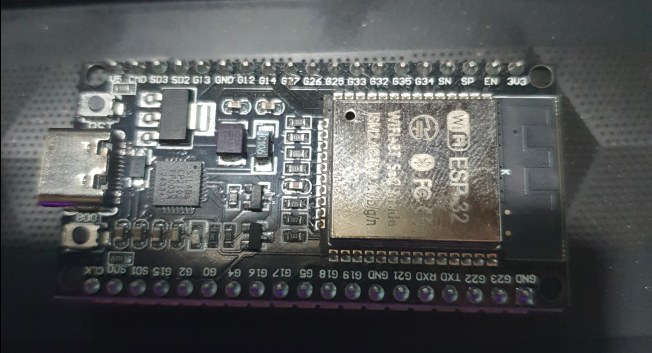
\includegraphics[width=0.56\textwidth]{figures/eespp.png}
\caption{Carte ESP32 utilisée pour le prototype ARGOS}
\label{fig-argos-esp32}
\end{figure}
\tablesourcepromoteurs

\subsubsection{Capteur de température et d'humidité}

Le firmware déclare un AM2302/DHT22 raccordé au GPIO~4. Il fournit les valeurs
\code{temperature} et \code{humidity} du message de télémétrie. Toute
conclusion sur sa précision doit être fondée sur un étalonnage ou sur la fiche
technique exacte du composant monté.

\begin{figure}[!htbp]
\centering
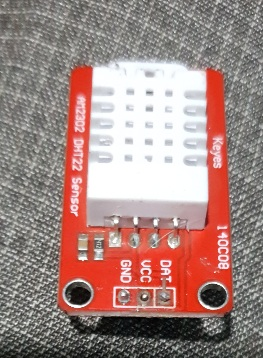
\includegraphics[width=0.26\textwidth]{figures/dht22.jpg}
\caption{Capteur de température et d'humidité}
\label{fig-argos-am2302}
\end{figure}
\tablesourcepromoteurs

\subsubsection{Pression, mouvement et détection de choc}

Le MPU-6050 est raccordé au bus I²C, SDA sur GPIO~8 et SCL sur GPIO~9. Le choc
instantané est exprimé en multiples de l'accélération de la pesanteur :
\begin{equation}
 a_m=\sqrt{a_x^2+a_y^2+a_z^2},\qquad
 choc=\frac{|a_m-g|}{g},\quad g=\SI{9.80665}{\metre\per\second\squared}.
\end{equation}
Une calibration des biais, un filtrage et la conservation du maximum sur une
courte fenêtre sont nécessaires pour limiter les faux positifs. La vitesse de
référence provient du GNSS. Une intégration de l'accélération horizontale du
MPU peut seulement combler une brève perte GNSS, car la dérive rend une vitesse
calculée uniquement par centrale inertielle rapidement inexploitable.

La pression atmosphérique nécessite l'ajout d'un BME280 ou BMP280 sur le même
bus I²C. Jusqu'à cette intégration, la valeur envoyée par le firmware est une
constante de compatibilité et non une observation du milieu.

\begin{figure}[!htbp]
\centering
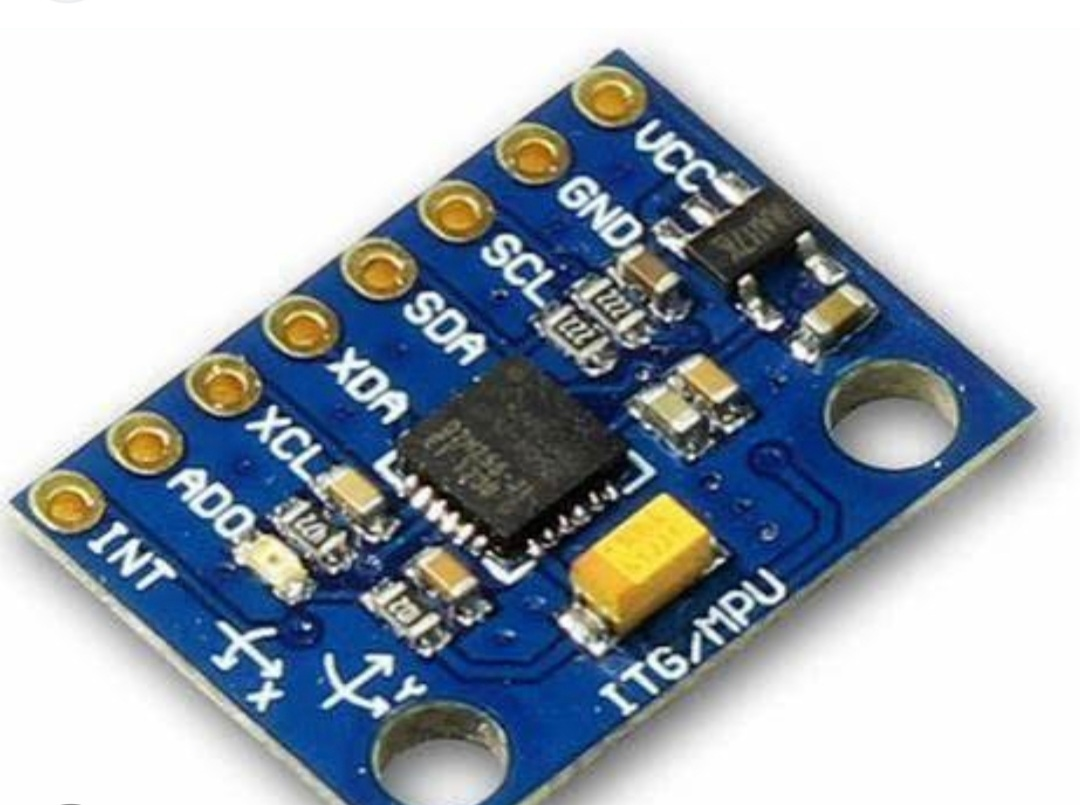
\includegraphics[width=0.26\textwidth]{figures/sda.jpg}
\caption{Pression, mouvement et détection de choc}
\label{fig-argos-BME}
\end{figure}
\tablesourcepromoteurs

\subsubsection{Détection de flamme et acquisition audio}

Le détecteur de flamme est raccordé au GPIO~21 et le microphone analogique au
GPIO~5. Le niveau sonore est inclus dans la télémétrie. Pour produire un son
lisible, le firmware doit échantillonner le signal, construire un fichier WAV,
le conserver temporairement sur la microSD puis l'envoyer à
\code{/api/iot/audio}. Le backend limite actuellement un fichier à 25~Mio,
calcule son empreinte SHA-256 et le place dans le stockage privé. Un découpage
en segments de 5 à 30 secondes fournit un quasi-direct compatible avec les
coupures réseau ; ce mécanisme ne constitue pas un flux audio continu.

\begin{figure}[!htbp]
\centering
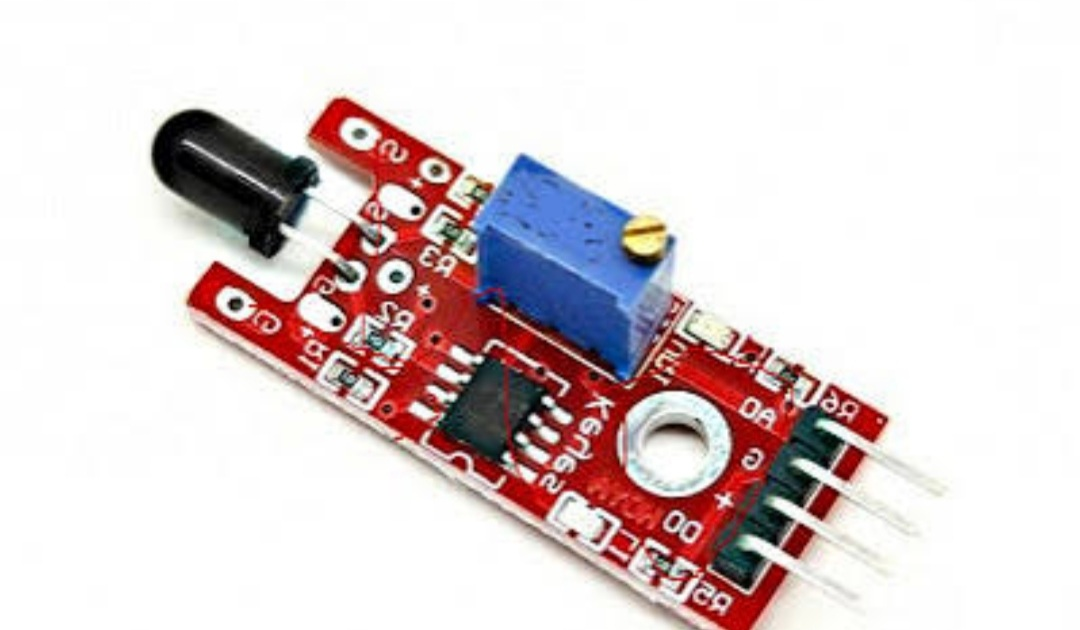
\includegraphics[width=0.26\textwidth]{figures/fl.jpg}
\caption{Module de Détection de flamme}
\label{fig-argos-flamme}
\end{figure}
\tablesourcepromoteurs

\subsubsection{Module de géolocalisation}

Le NEO-6M communique avec l'ESP32 par UART : TX du GPS vers GPIO~17 et RX du
GPS vers GPIO~18. TinyGPS++ interprète les trames et fournit latitude,
longitude, vitesse et cap. Les coordonnées alimentent directement les tables
de positions et le marqueur Leaflet de la boîte noire. En l'absence de position
valide, la donnée doit être qualifiée comme indisponible et la dernière
position valide peut être affichée avec son horodatage.

\begin{figure}[!htbp]
\centering
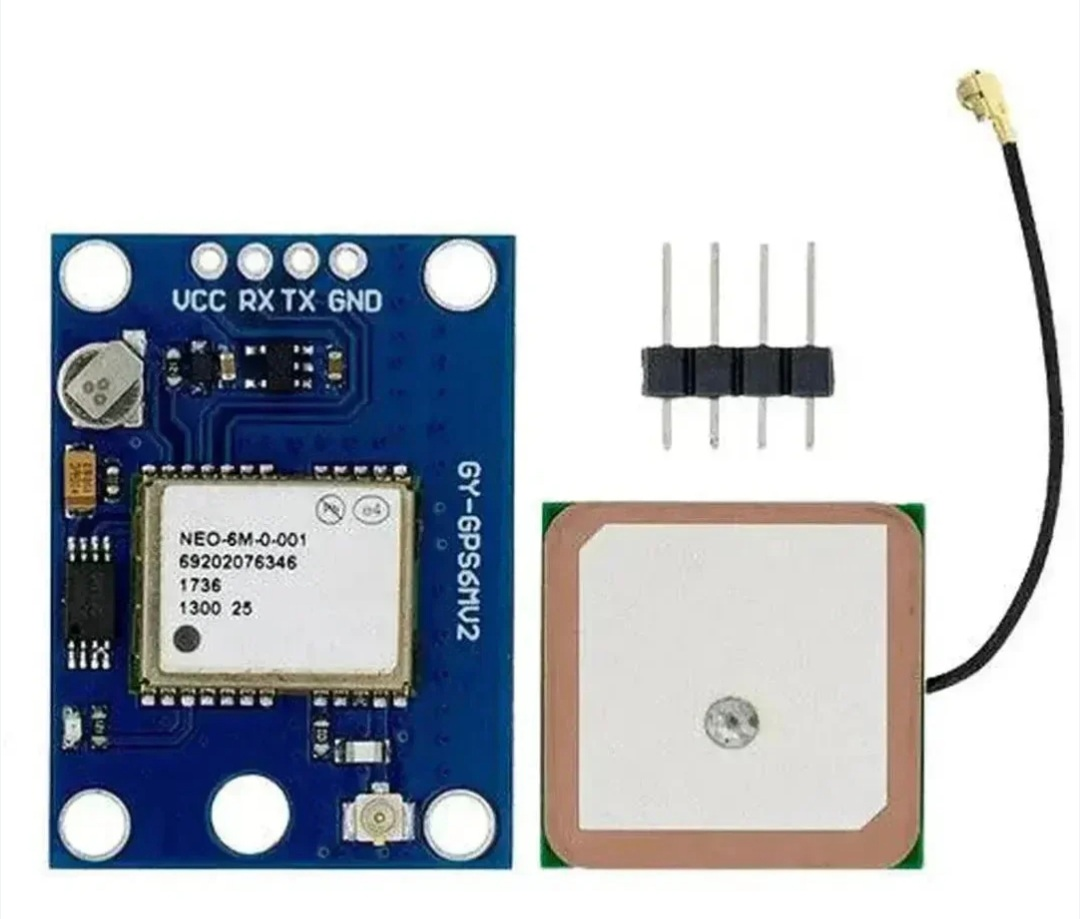
\includegraphics[width=0.26\textwidth]{figures/asp.jpg}
\caption{Module GPS du prototype ARGOS}
\label{fig-argos-gps}
\end{figure}
\tablesourcepromoteurs

\subsubsection{Alimentation et signalisation}

La LED bleue est raccordée au GPIO~1 et le buzzer actif au GPIO~10. La LED
indique que le Wi-Fi, l'identité du boîtier, son affectation, le MPU-6050 et la
carte SD sont opérationnels. Le choix définitif de la batterie, du régulateur, des
protections et du boîtier doit être documenté à partir du montage réellement
assemblé. L'autonomie ne doit être annoncée qu'après mesure du courant dans
les différents modes.

\begin{figure}[!htbp]
\centering
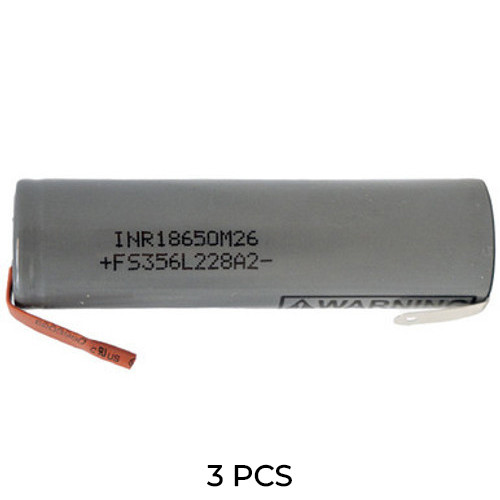
\includegraphics[width=0.26\textwidth]{figures/pile.jpg}
\caption{Alimentation}
\label{fig-argos-alimentation}
\end{figure}
\tablesourcepromoteurs


\section{Processus de réalisation}
\subsection{Connectivité terrestre et maritime}

Le Wi-Fi demeure le canal du prototype de laboratoire et de la configuration
locale. Pour l'exploitation mobile internationale, l'architecture retient une
stratégie multiréseau :
\begin{itemize}
    \item LTE-M ou NB-IoT avec profil eSIM et itinérance multi-opérateurs pour
    les zones terrestres et portuaires couvertes ;
    \item LoRaWAN pour les ports, entrepôts et corridors équipés de passerelles,
    avec itinérance entre opérateurs lorsqu'elle est contractuellement disponible ;
    \item satellite IoT à faible débit comme secours en mer et dans les zones
    isolées dépourvues de couverture terrestre.
\end{itemize}

LoRaWAN est une technologie longue portée et basse consommation, mais sa
couverture internationale dépend d'infrastructures de passerelles et de
réseaux interconnectés. Le satellite complète donc LoRaWAN et les réseaux
cellulaires ; il n'est sollicité que pour les messages prioritaires afin de
maîtriser l'énergie, le débit et le coût. Le firmware place les messages non
confirmés dans une file sur microSD, conserve une séquence croissante et les
retransmet après le rétablissement d'un canal.

\begin{figure}[!htbp]
\centering
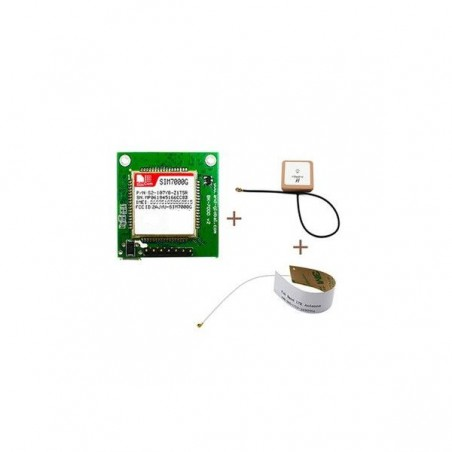
\includegraphics[width=0.56\textwidth]{figures/sim.jpg}
\caption{Sim 800l LTE-4G}
\label{fig-argos-sim}
\end{figure}
\tablesourcepromoteurs


\subsection{Schéma de raccordement}

Le schéma de raccordement formalise l'architecture matérielle et les interconnexions physiques du prototype ARGOS, articulé autour de la carte microcontrôlée principale et de ses périphériques capteurs. Cette vue d'ensemble est essentielle pour garantir la conformité du montage électronique, la fiabilité des transmissions de données et l'alimentation stable des composants embarqués en condition réelle.

\begin{figure}[!htbp]
\centering
\resizebox{0.85\textwidth}{!}{%
  \resizebox{0.98\linewidth}{!}{%
\begin{tikzpicture}[font=\sffamily\scriptsize,
 module/.style={draw=argosnavy,rounded corners=2pt,align=left,minimum width=4cm,minimum height=.9cm,fill=white},
 mcu/.style={draw=argosnavy,rounded corners=2pt,align=center,minimum width=4.2cm,minimum height=7cm,fill=argoslight,line width=1.1pt},
 wire/.style={draw=argosmid,line width=.8pt}]
\node[mcu] (mcu) at (0,0) {\textbf{ESP32}\\[3pt]
GPIO 1 : LED\\\\GPIO 4 : DHT22 (ou autre)\\GPIO 5 : SCL (I²C)\\
GPIO 13 : buzzer\\GPIO 14 : MOSI (SD)\\GPIO 15 : RX (GPS)\\GPIO 16 : ECHO (HC-SR04)\\
GPIO 17 : flamme\\GPIO 18 : TRIG (HC-SR04)\\GPIO 21 : SDA (I²C)\\GPIO 22 : microphone\\
GPIO 26 : SCK (SD)\\GPIO 27 : MISO (SD)};
\node[module] (dht) at (-7,3.3) {DHT22 : DATA $\rightarrow$ GPIO 4};
\node[module] (analog) at (-7,1.9) {Microphone : GPIO 22};
\node[module] (ultra) at (-7,.5) {HC-SR04 : TRIG 18, ECHO 16\footnotemark};
\node[module] (i2c) at (-7,-.9) {MPU-6050 + BME280 : SDA 21, SCL 5};
\node[module] (alarm) at (-7,-2.3) {LED / Buzzer / Flamme : GPIO 1 / 13 / 17};
\node[module] (sd) at (7,3.3) {microSD SPI : MOSI 14, SCK 26, MISO 27};
\node[module] (modem) at (7,1.4) {Modem LTE-M/NB-IoT ou LoRaWAN};
\node[module] (gnss) at (7,-.5) {NEO-6M UART : TX $\rightarrow$ 2, RX $\leftarrow$ 15};
\node[module] (sat) at (7,-2.4) {Modem satellite IoT\\UART/SPI selon module};
\foreach \n in {dht,analog,ultra,i2c,alarm} \draw[wire] (\n.east) -- (mcu.west |- \n.east);
\foreach \n in {sd,modem,gnss,sat} \draw[wire] (mcu.east |- \n.west) -- (\n.west);
\end{tikzpicture}%
}
\footnotetext{La sortie ECHO 5 V du HC-SR04 doit être abaissée à 3,3 V par pont diviseur ou convertisseur de niveau.}%
}
\caption{Schéma de raccordement logique du prototype ARGOS}
\label{fig-argos-cablage}
\end{figure}
\tablesourcepromoteurs

Le dispositif repose principalement sur le module ESP32-S3, qui centralise l'acquisition des données métrologiques et géographiques. Les bus de communication numérique (I2C et SPI) interconnectent les capteurs de position, d'inertie et environnementaux, tandis que les interfaces spécifiques gèrent le module de téléphonie mobile et les capteurs analogiques. Cette disposition modulaire assure une maintenance aisée du prototype tout en garantissant l'intégrité des signaux électriques face aux perturbations électromagnétiques rencontrées sur le terrain.

\par Le schéma de la \cref{fig-argos-cablage} présente les raccordements définis
dans le firmware. Les traits orientés représentent les signaux d'entrée ou de
sortie. Les liaisons d'alimentation sont séparées des données. Avant la mise
sous tension, il est indispensable de vérifier la tension admissible de
chaque module, de partager une masse commune et d'empêcher qu'une entrée
analogique reçoive une tension supérieure à la limite de l'ESP32.

\begin{figure}[!htbp]
\centering
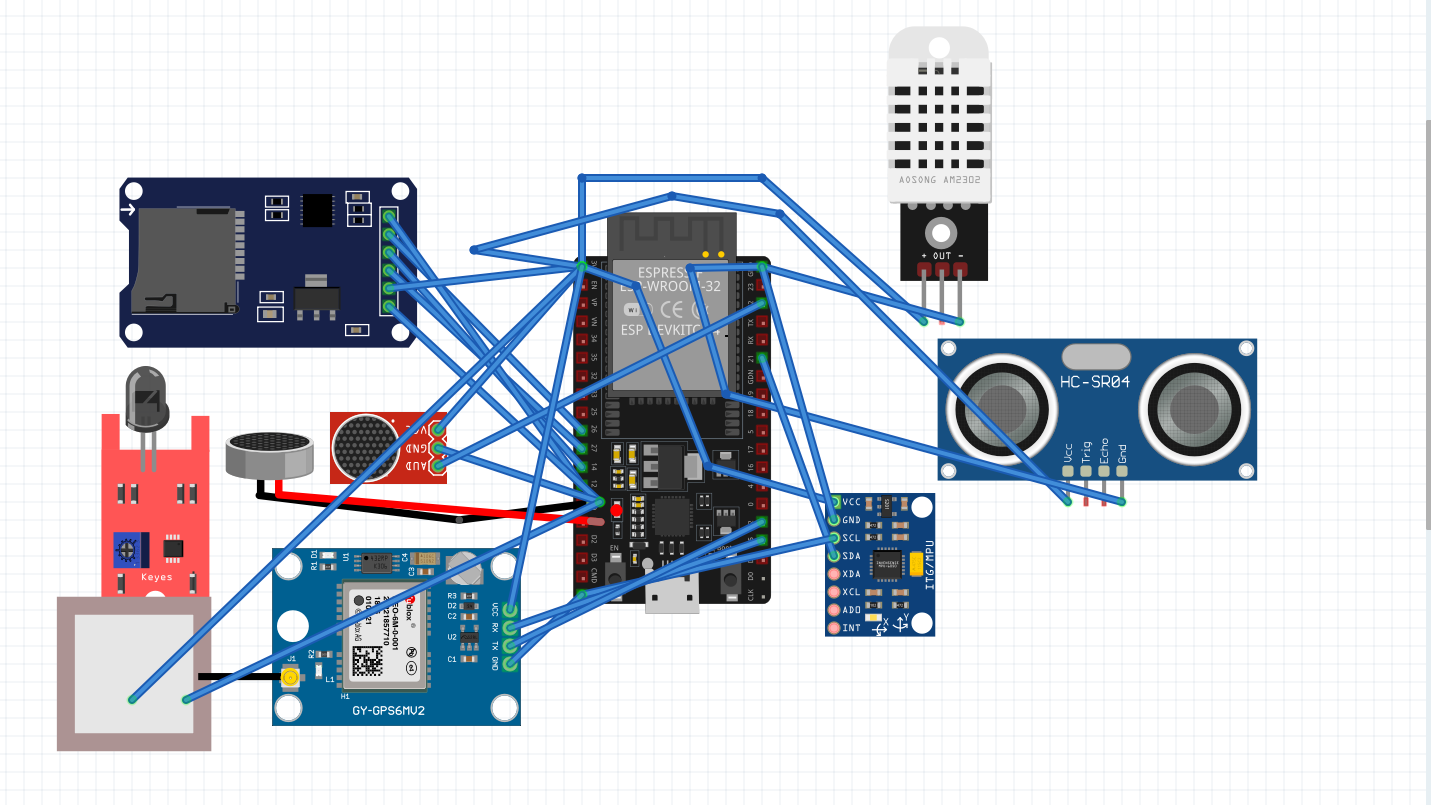
\includegraphics[width=0.86\textwidth]{figures/platine_de.png}
\caption{Vue générale du câblage réel}
\label{fig-cablages-jumpeur}
\end{figure}
\tablesourcepromoteurs

\begin{figure}[!htbp]
\centering
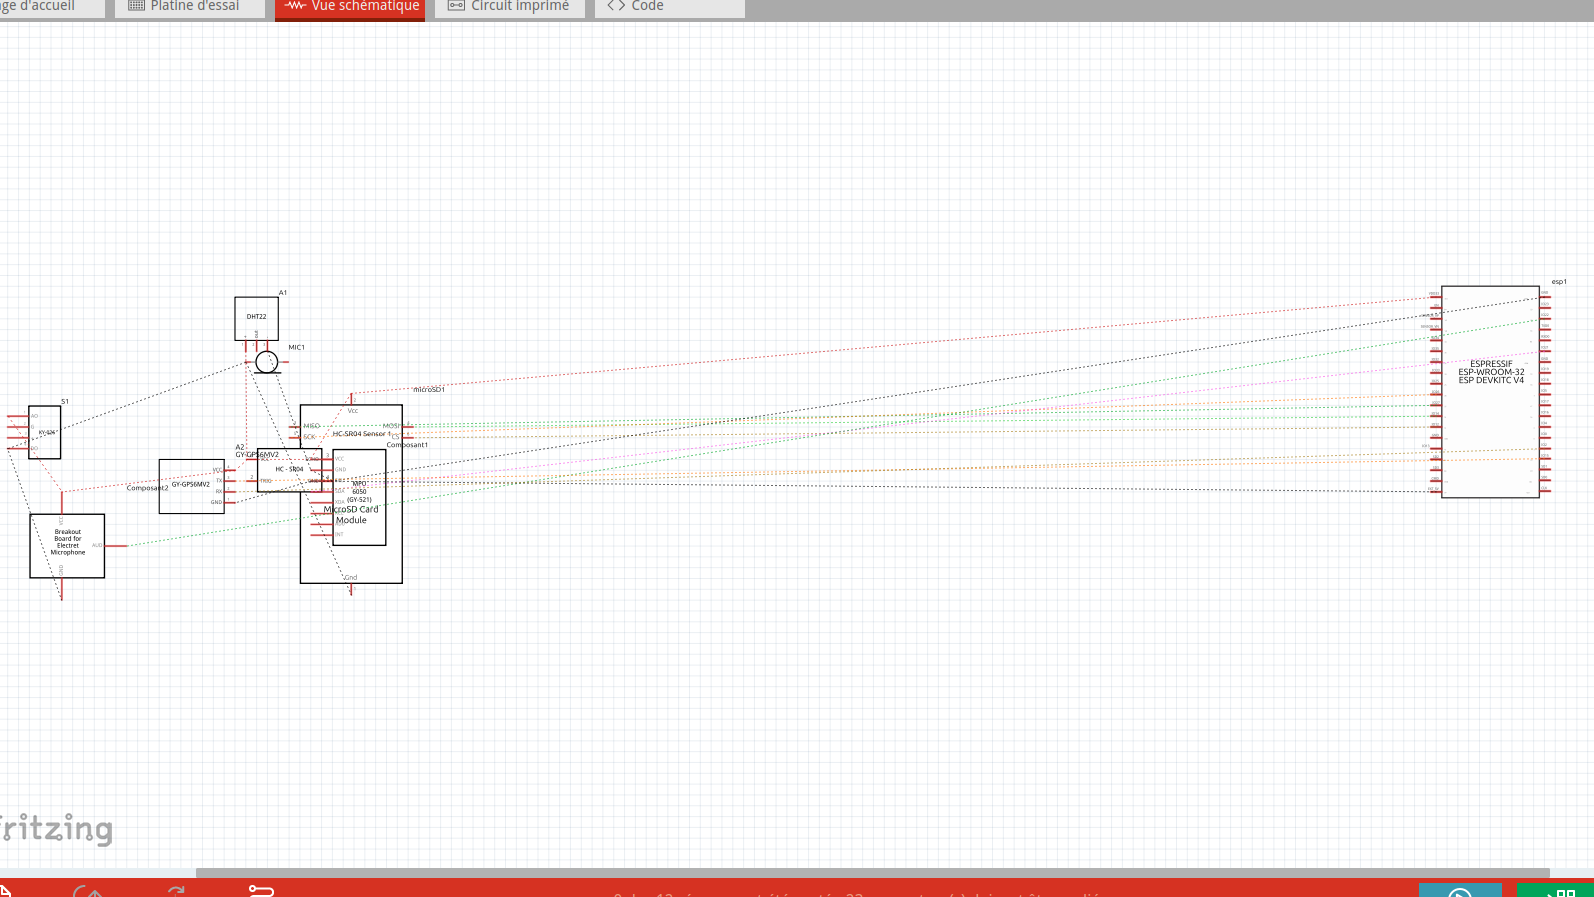
\includegraphics[width=0.86\textwidth]{figures/shemat.png}
\caption{Vue générale du câblage imprimé}
\label{fig-cablages-imprimer}
\end{figure}
\tablesourcepromoteurs


\subsection{Organisation du firmware}

Cette section décrit le fonctionnement interne du micrologiciel embarqué sur l'ESP32, depuis son initialisation jusqu'à la construction et l'envoi des messages de télémétrie. Elle détaille les principales étapes exécutées par le programme, notamment la mise en route des différents modules, l'enrôlement du dispositif et la collecte des mesures issues des capteurs. Cette présentation permet de comprendre comment les données physiques acquises par le prototype sont transformées en informations exploitables par la plateforme.

\subsubsection{Initialisation}

Au démarrage, le programme initialise les interfaces série, I²C et SPI, les
broches, le DHT22, le MPU-6050, la microSD, le GNSS et le canal réseau. Lors du premier usage, la fonction
\code{enrollDevice()} envoie le \code{deviceUid} et le jeton d'enrôlement à
\code{/api/iot/enroll}. Si la demande est acceptée, le serveur retourne une
clé permanente utilisée pour les échanges suivants.

\subsubsection{Acquisition et construction du message}

La fonction \code{sendTelemetry()} lit les capteurs et construit un document
JSON contenant :
\begin{itemize}
    \item un identifiant de message, l'identité du dispositif et une séquence ;
    \item la date, le type du message et la version implicite du protocole ;
    \item la position, la précision, la vitesse et le cap ;
    \item les mesures de température, humidité, choc, pression, niveau sonore,
    distance et accélérations triaxiales ;
    \item les indicateurs de flamme, porte, batterie et modes actifs.
\end{itemize}

Le message est envoyé à \code{/api/iot/telemetry} avec la clé du dispositif
dans l'en-tête \code{X-Device-Key}. Le serveur répond avec un code HTTP et un
résultat JSON affichés sur le port série.

\subsubsection{Commandes et audio}

Le backend expose la consultation de l'état, les commandes et la réception
d'un fichier audio authentifié. Il reconnaît les commandes
de sécurité, écoute, enregistrement, détection de flamme, demande de position,
demande d'état et alerte locale. Le cycle complet prévoit un accusé
\code{ACKNOWLEDGED}, puis un résultat final tel que \code{SUCCEEDED} ou
\code{FAILED}.

\subsection{Protocole d'intégration avec la plateforme}

L'intégration suit le cycle ci-dessous :
\begin{enumerate}
    \item création préalable d'une boîte noire dans ARGOS ;
    \item provisionnement du dispositif par un superadministrateur ou un
    propriétaire autorisé ;
    \item configuration du \code{deviceUid} et du jeton temporaire ;
    \item enrôlement du prototype et réception de la clé permanente ;
    \item transmission périodique de la télémétrie avec
    \code{blackBoxId}, \code{containerId}, UUID et séquence croissante ;
    \item transfert séparé des segments audio authentifiés ;
    \item validation, normalisation et stockage par le backend ;
    \item génération éventuelle d'un événement et d'une notification ;
    \item publication des commandes et retour des accusés de réception.
\end{enumerate}

En production, les échanges doivent utiliser TLS. La clé permanente ne doit
pas être écrite dans les journaux et doit être conservée dans une zone
persistante protégée. Un dispositif compromis peut être révoqué côté serveur.

\subsection{Présentation du prototype assemblé}

Les vues du montage documentent son organisation interne, son enveloppe et
son intégration au support de transport.

\begin{figure}[!htbp]
\centering
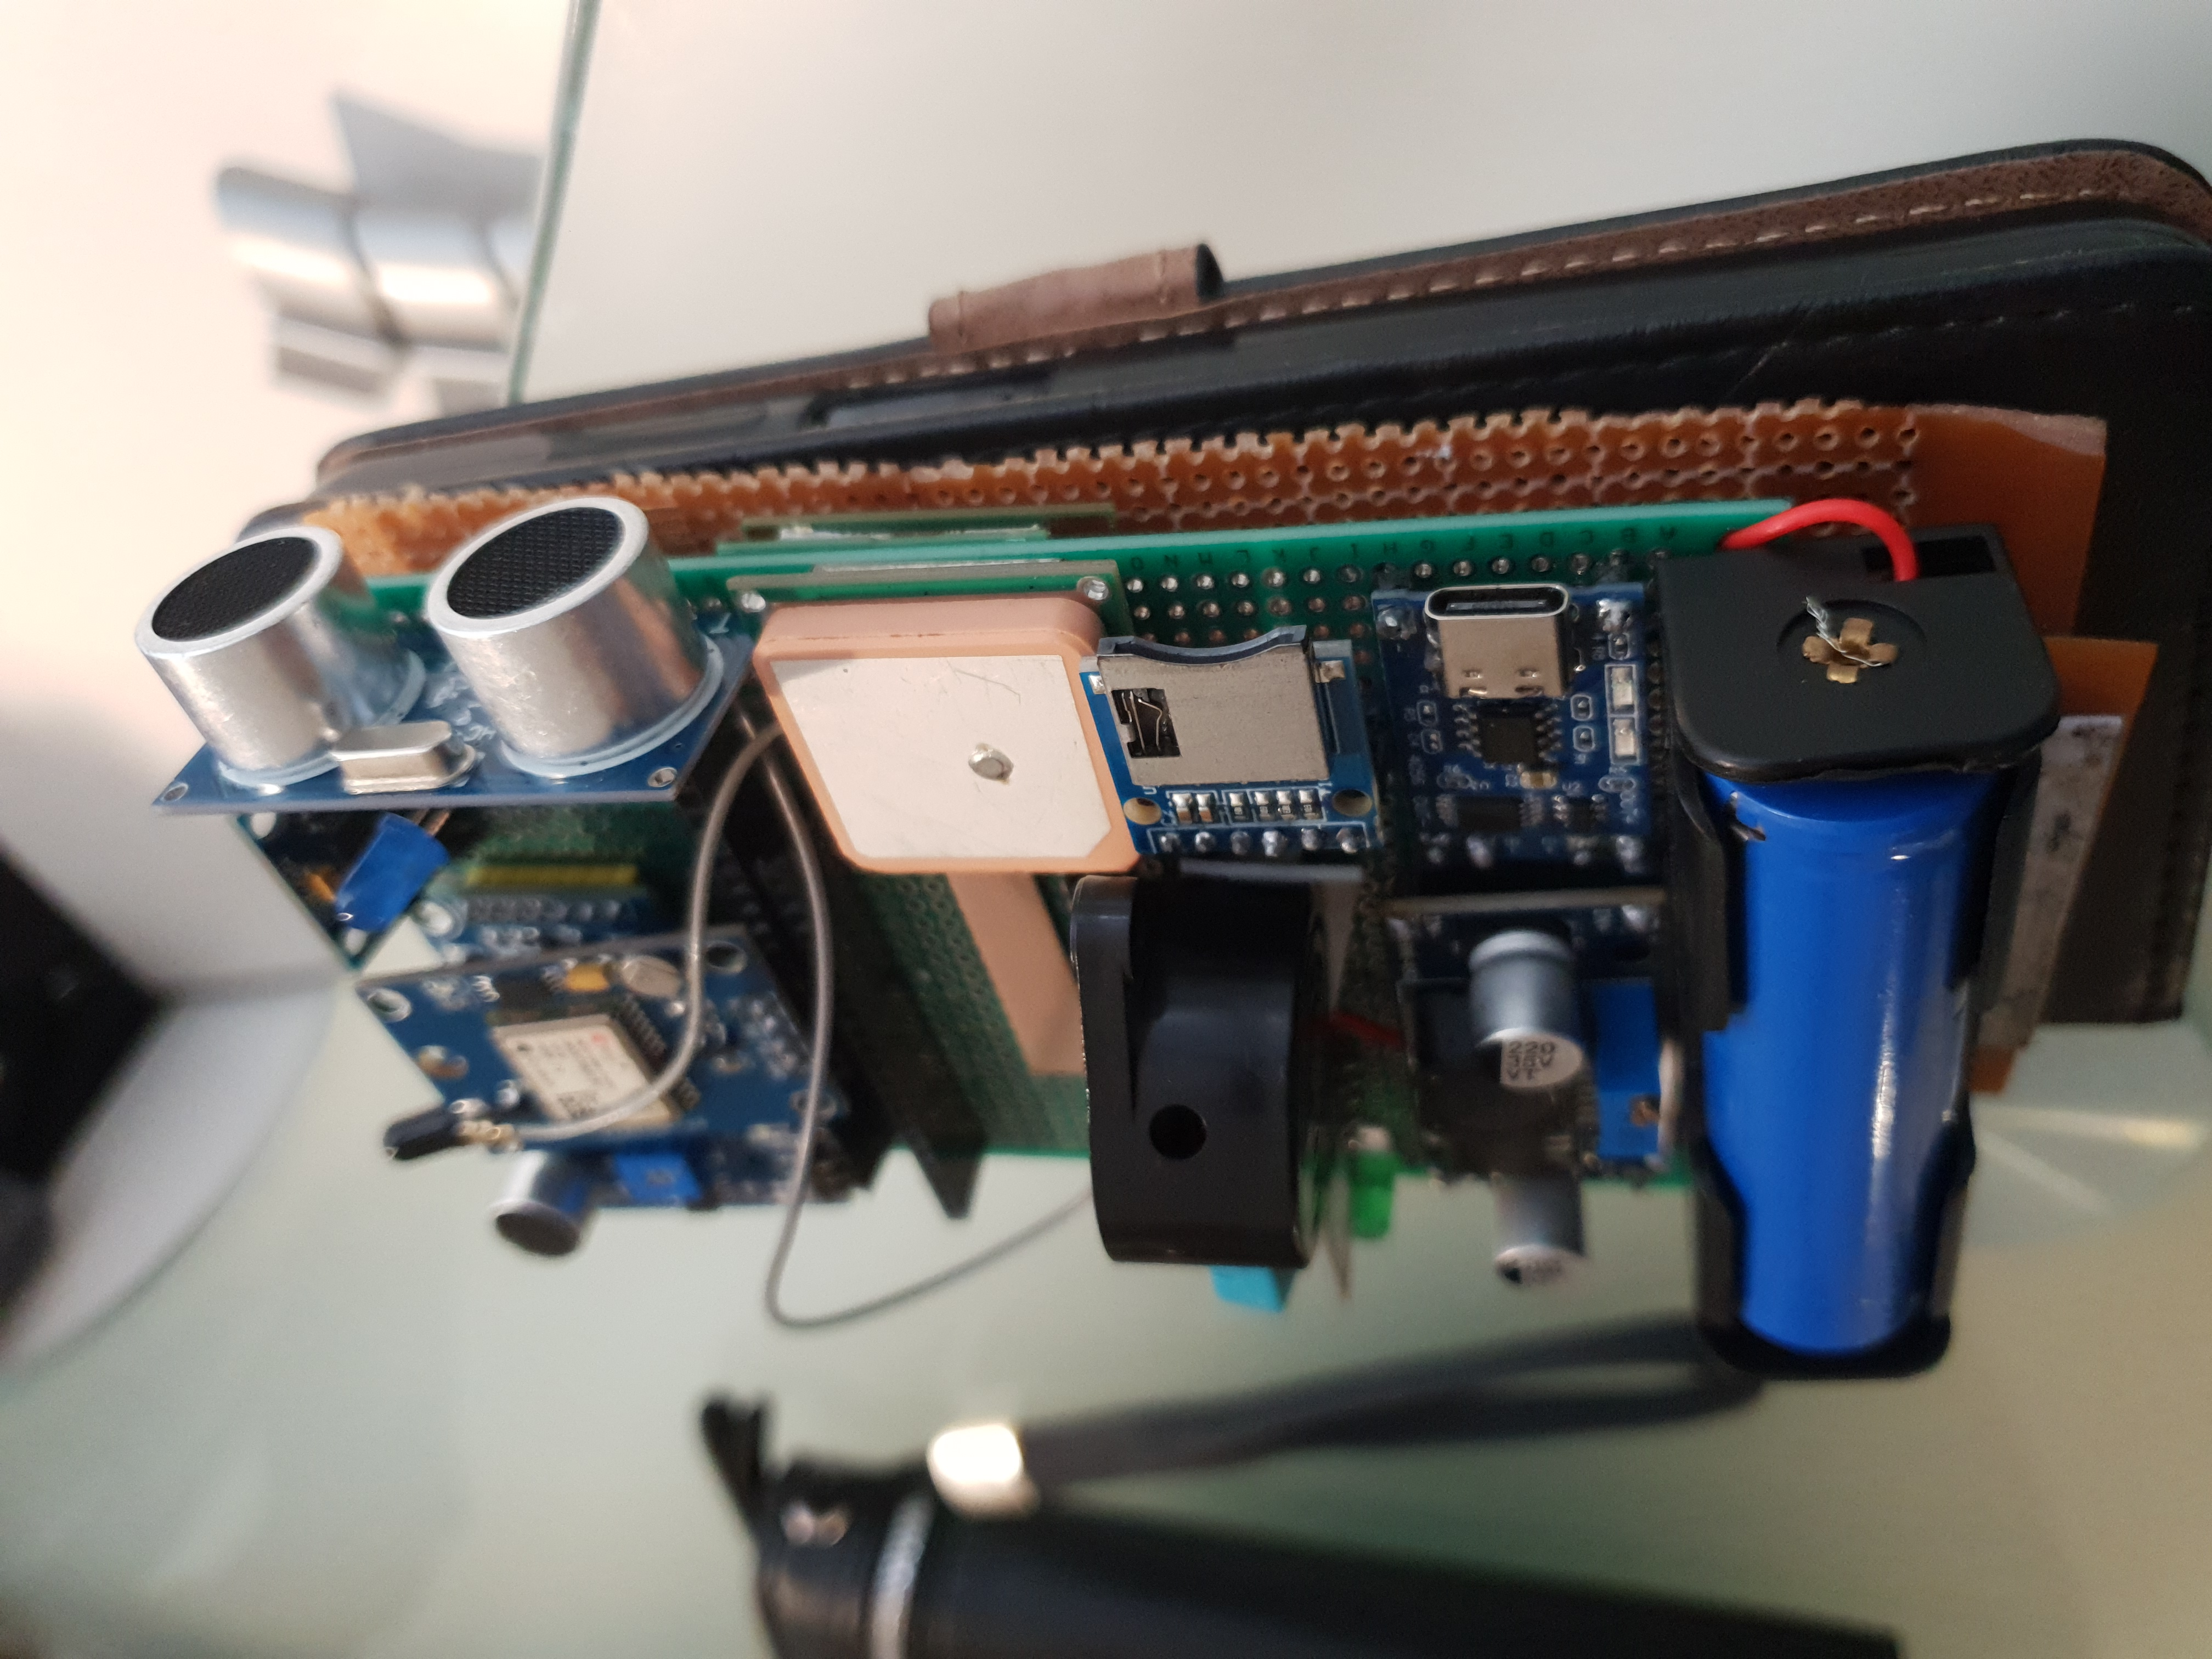
\includegraphics[width=0.86\textwidth, angle=180]{figures/argosint.png}
\caption{Vue interne du prototype ARGOS assemblé}
\label{fig-prototype-argos-interieur}
\end{figure}
\tablesourcepromoteurs

\begin{figure}[!htbp]
\centering
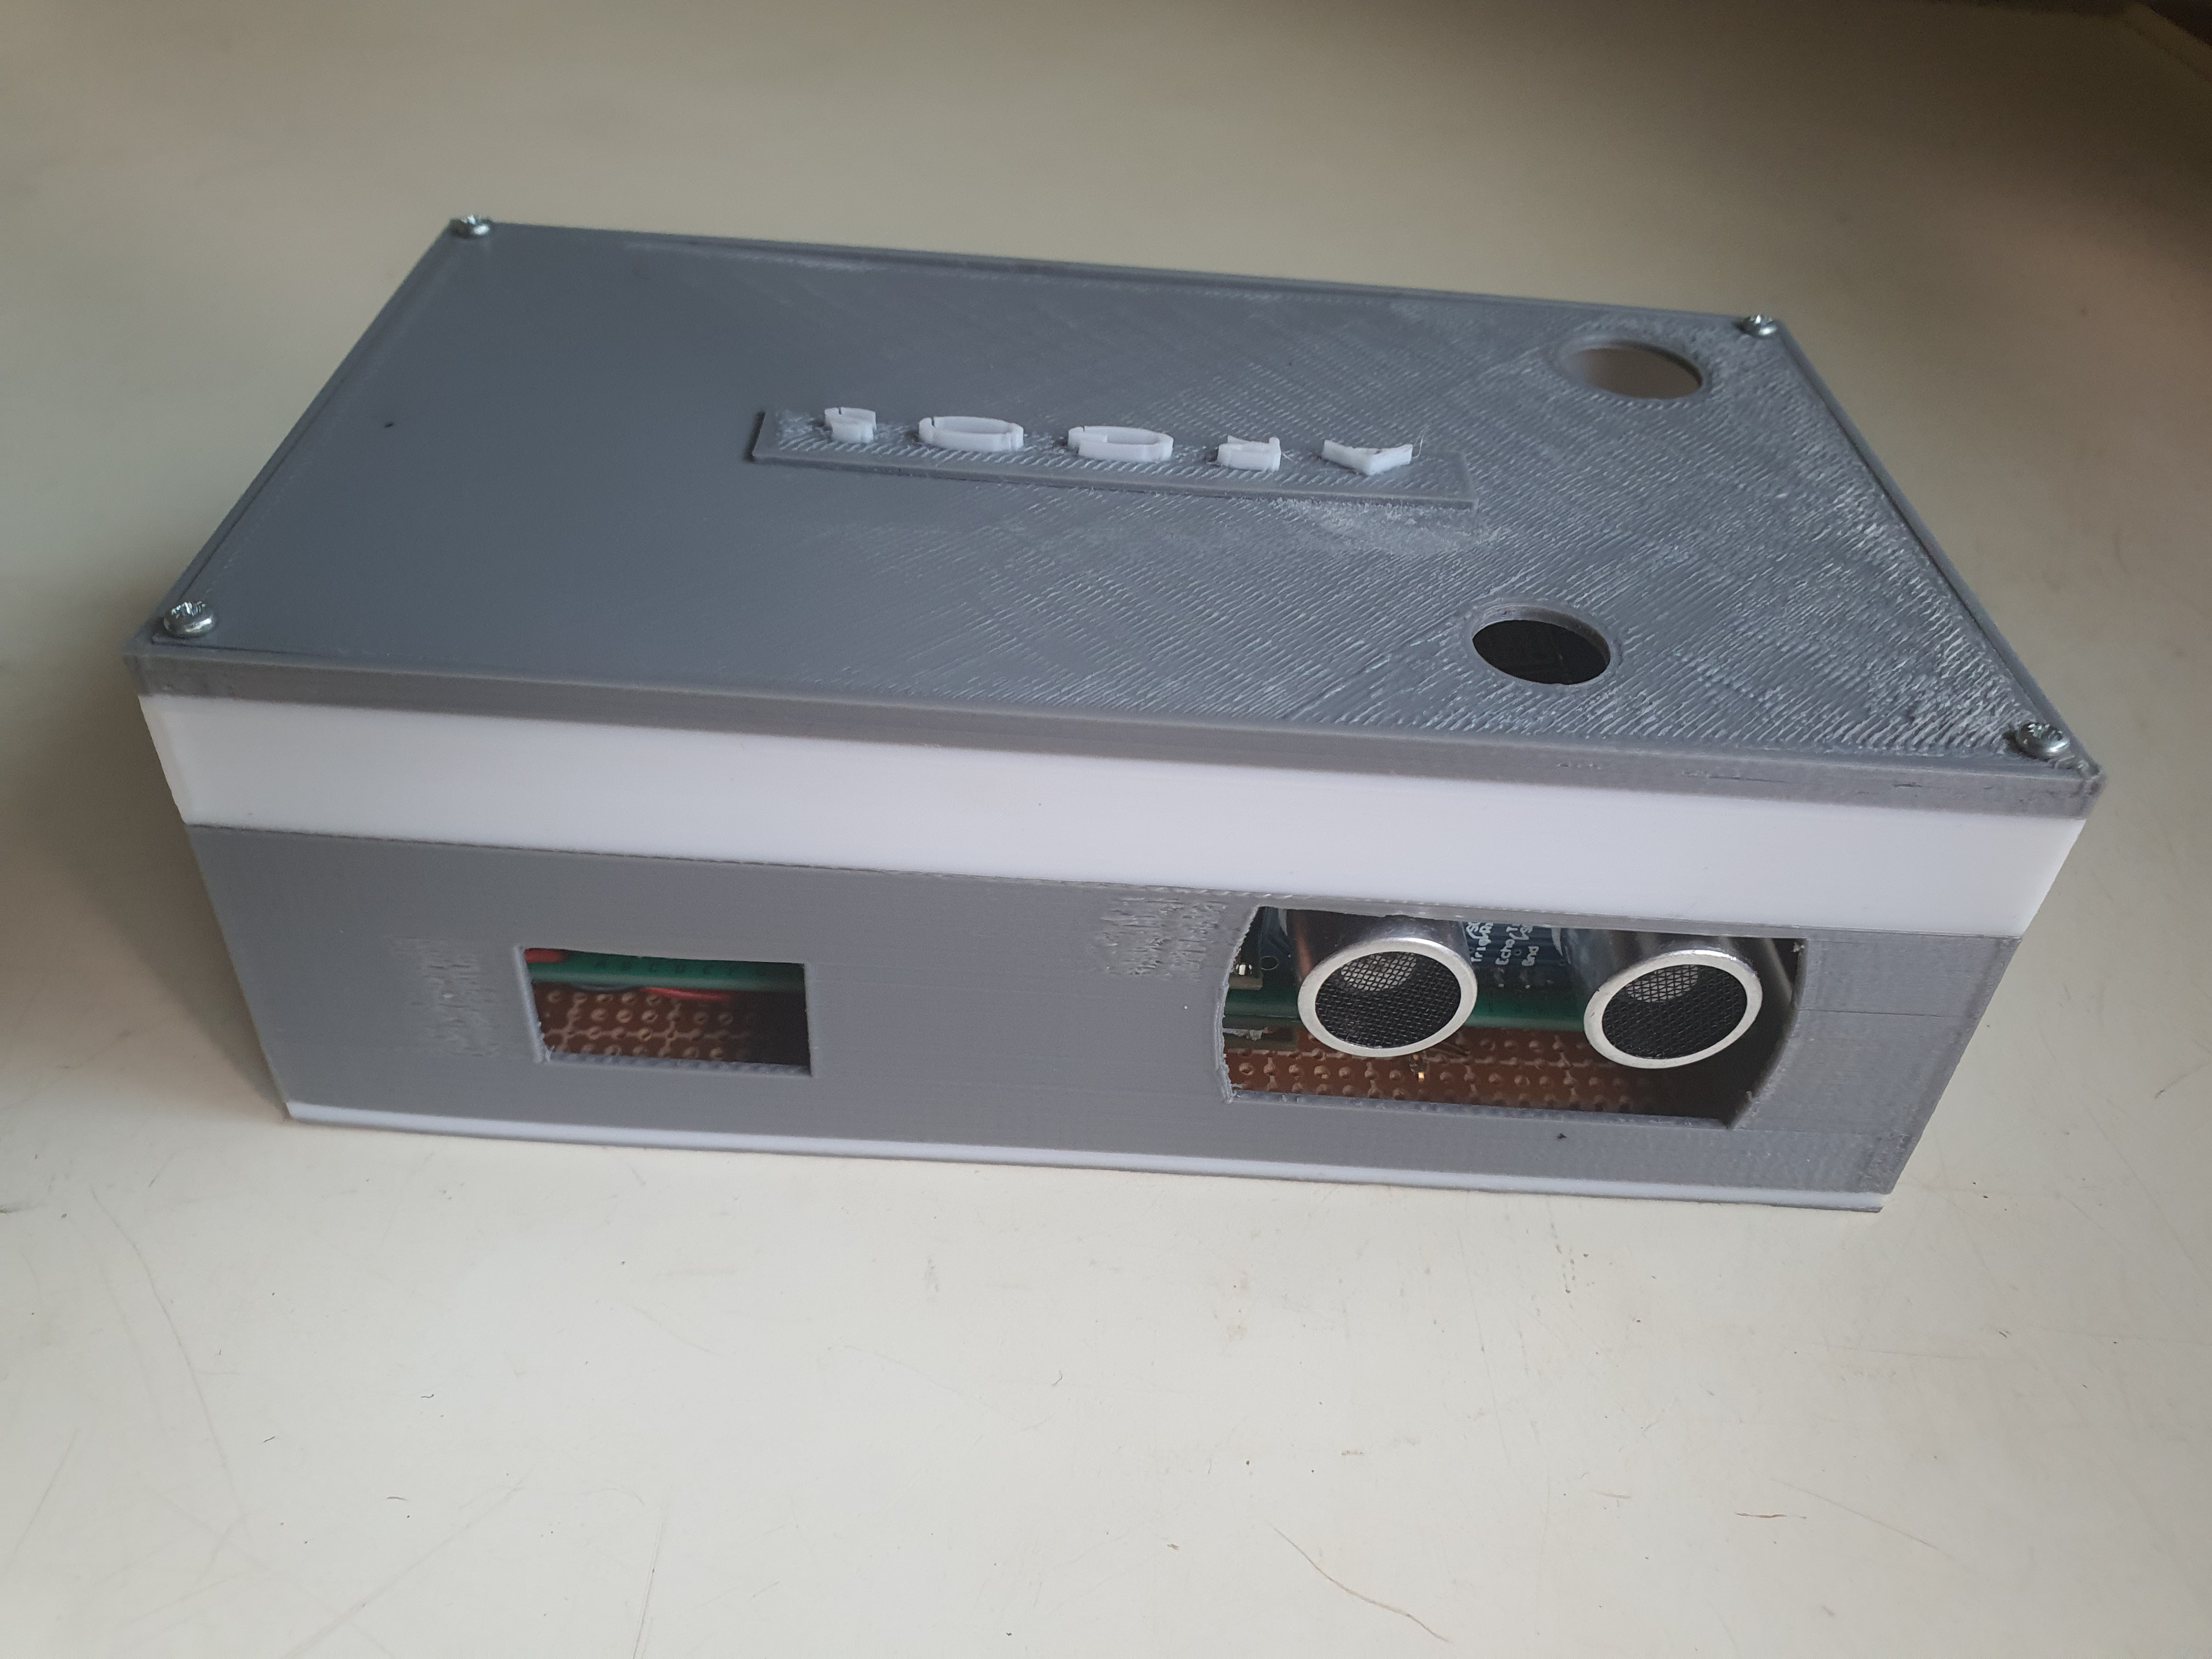
\includegraphics[width=0.86\textwidth]{figures/argosface.png}
\caption{Aspect extérieur du prototype ARGOS}
\label{fig-prototype-argos-exterieur}
\end{figure}
\tablesourcepromoteurs

\subsection{Interfaces de démonstration}

Les interfaces web permettent de vérifier visuellement le résultat des
traitements : authentification, affichage des conteneurs, carte, alertes,
boîtes noires et statistiques.

\begin{figure}[!htbp]
\centering
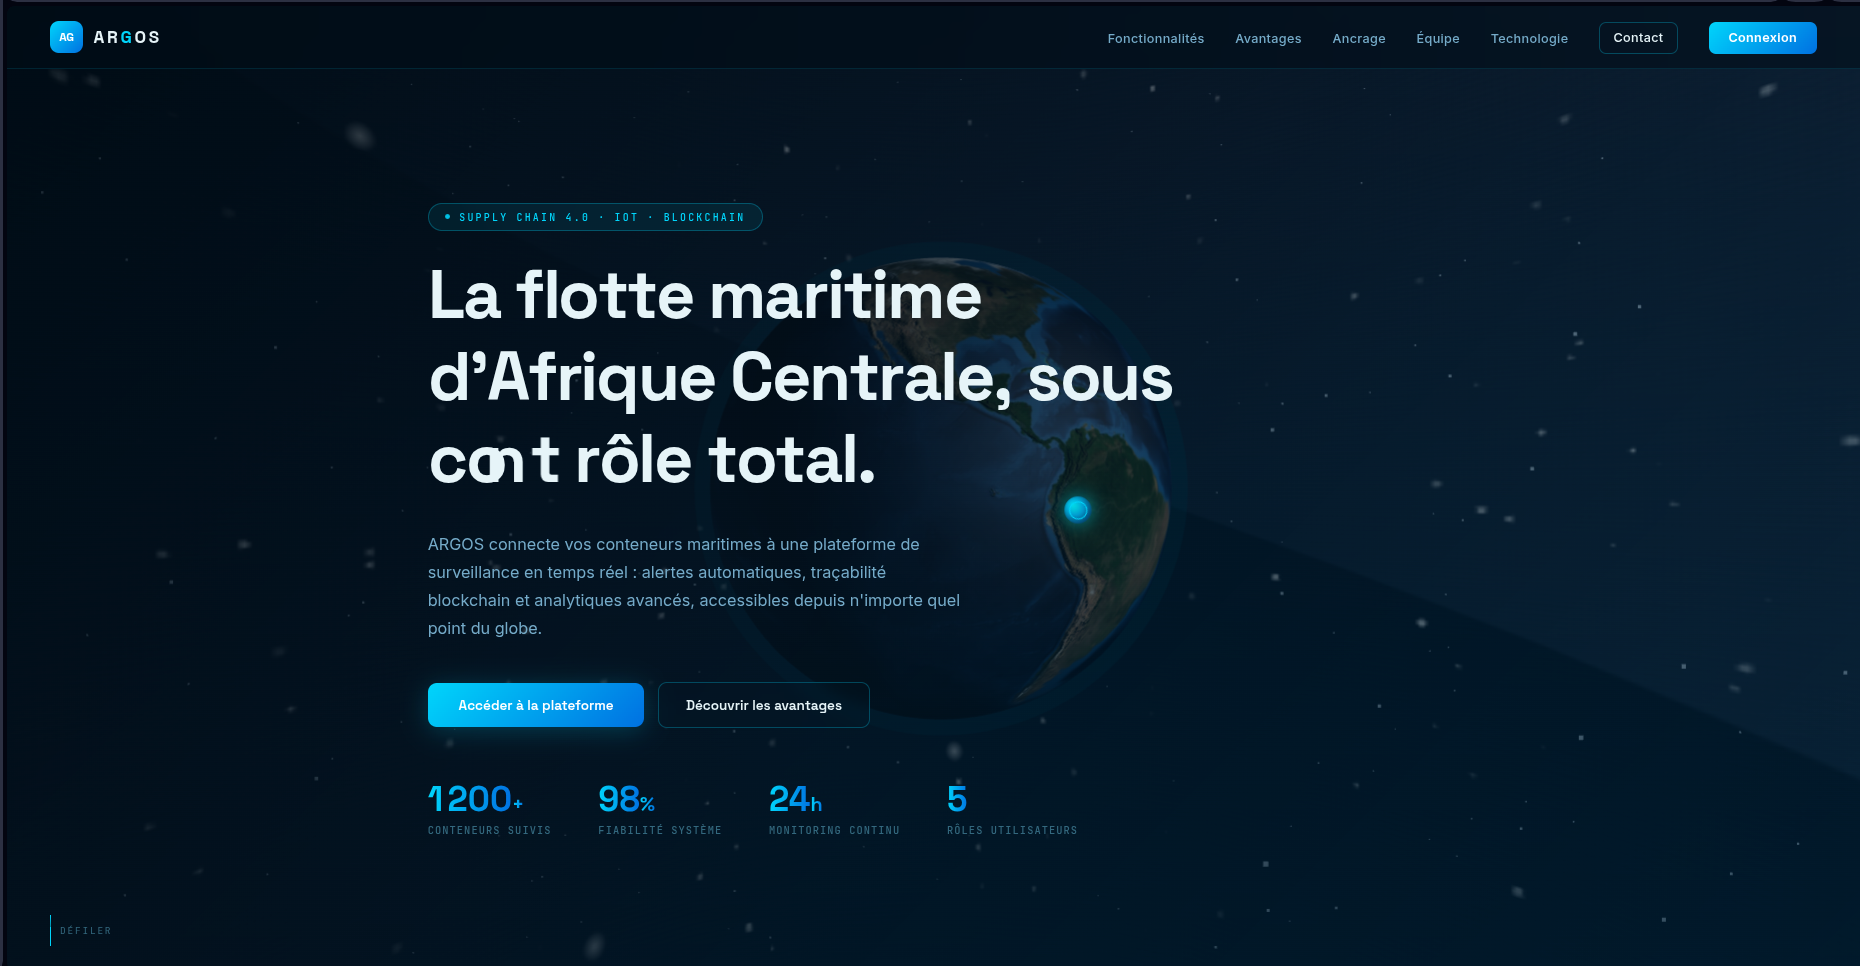
\includegraphics[width=0.66\textwidth]{figures/vitrine.png}
\caption{Page publique de présentation d'ARGOS}
\label{fig-vitrine-argos}
\end{figure}
\tablesourcepromoteurs

\begin{figure}[!htbp]
\centering
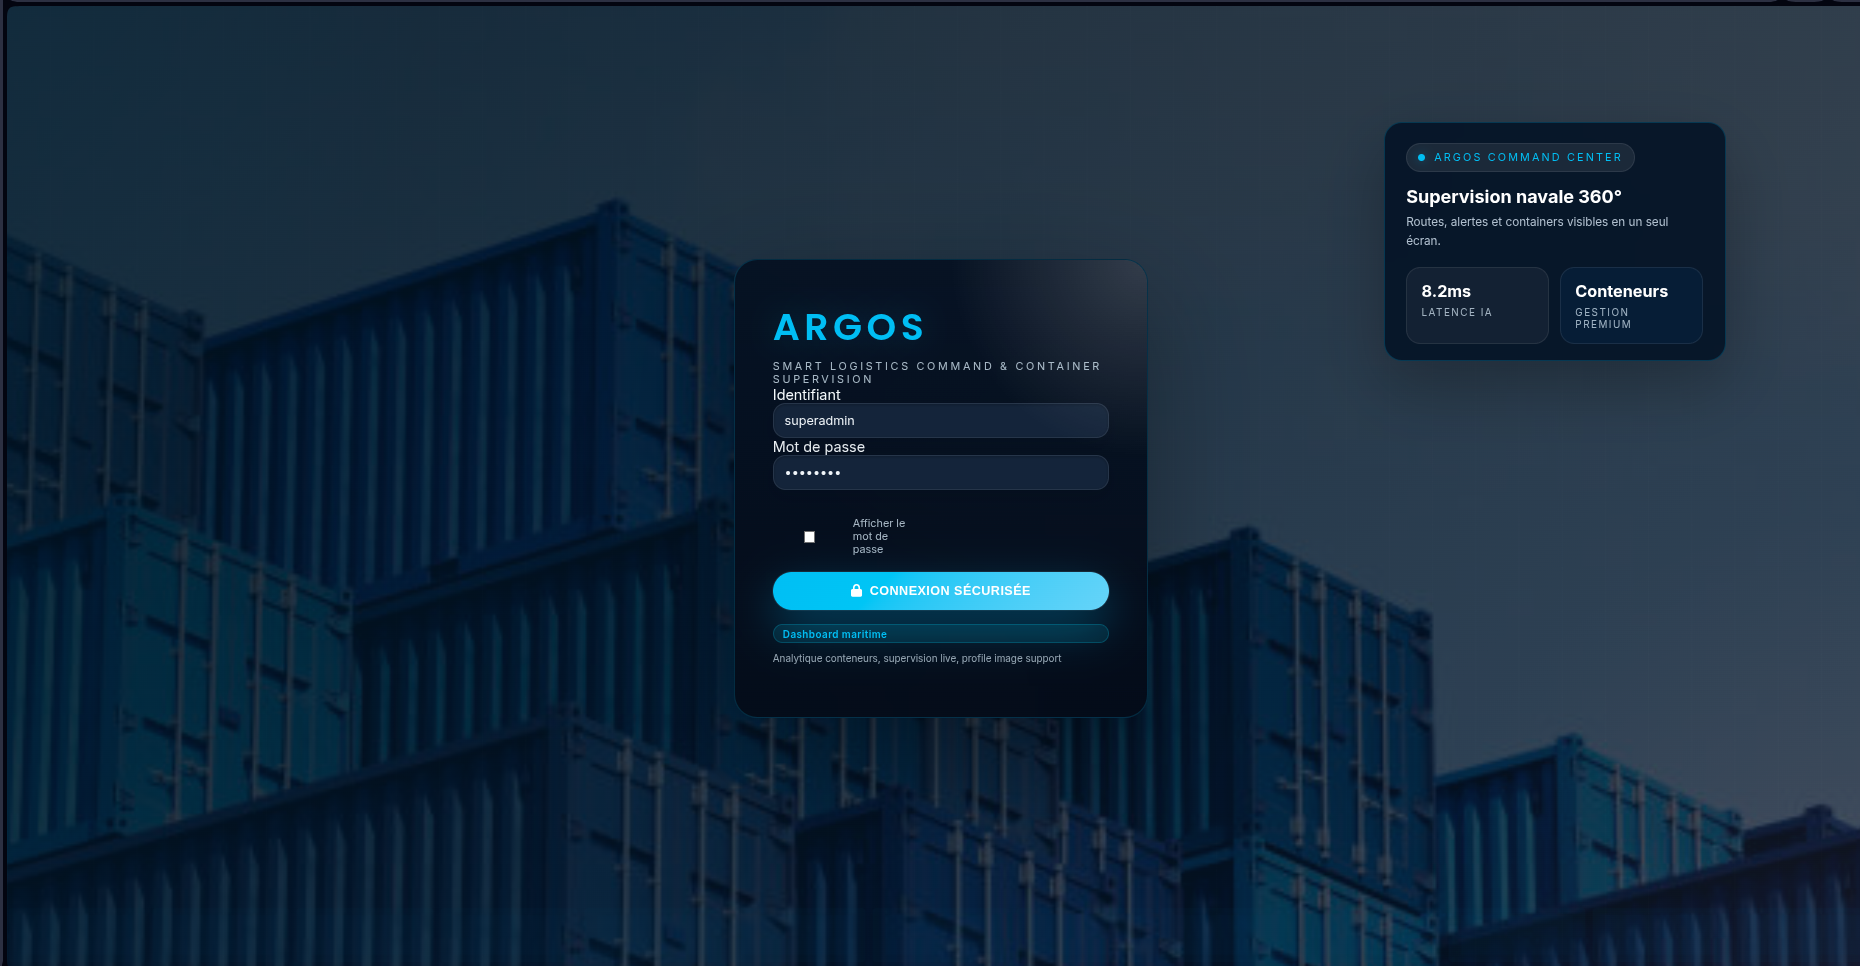
\includegraphics[width=0.66\textwidth]{figures/log.png}
\caption{Interface d'authentification d'ARGOS}
\label{fig-auth-argos}
\end{figure}
\tablesourcepromoteurs

\begin{figure}[!htbp]
\centering
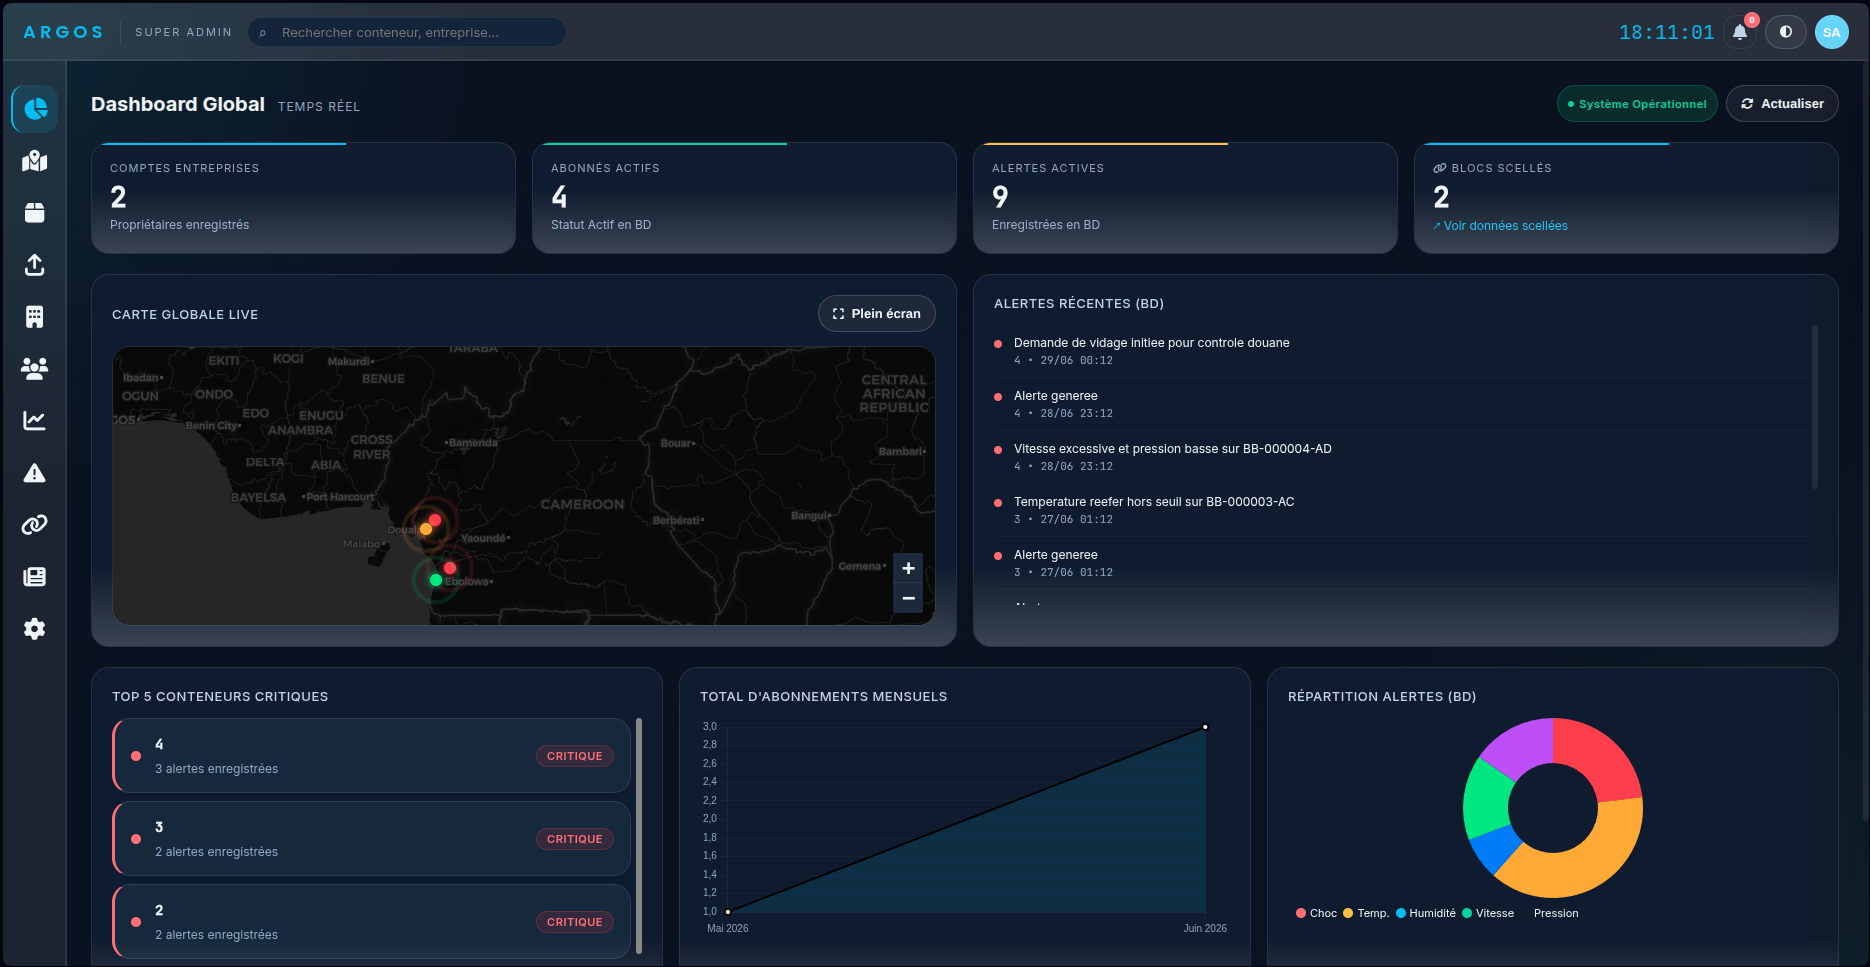
\includegraphics[width=0.66\textwidth]{figures/dash.png}
\vspace{0.5cm} % Petit espace ajouté pour séparer les deux images
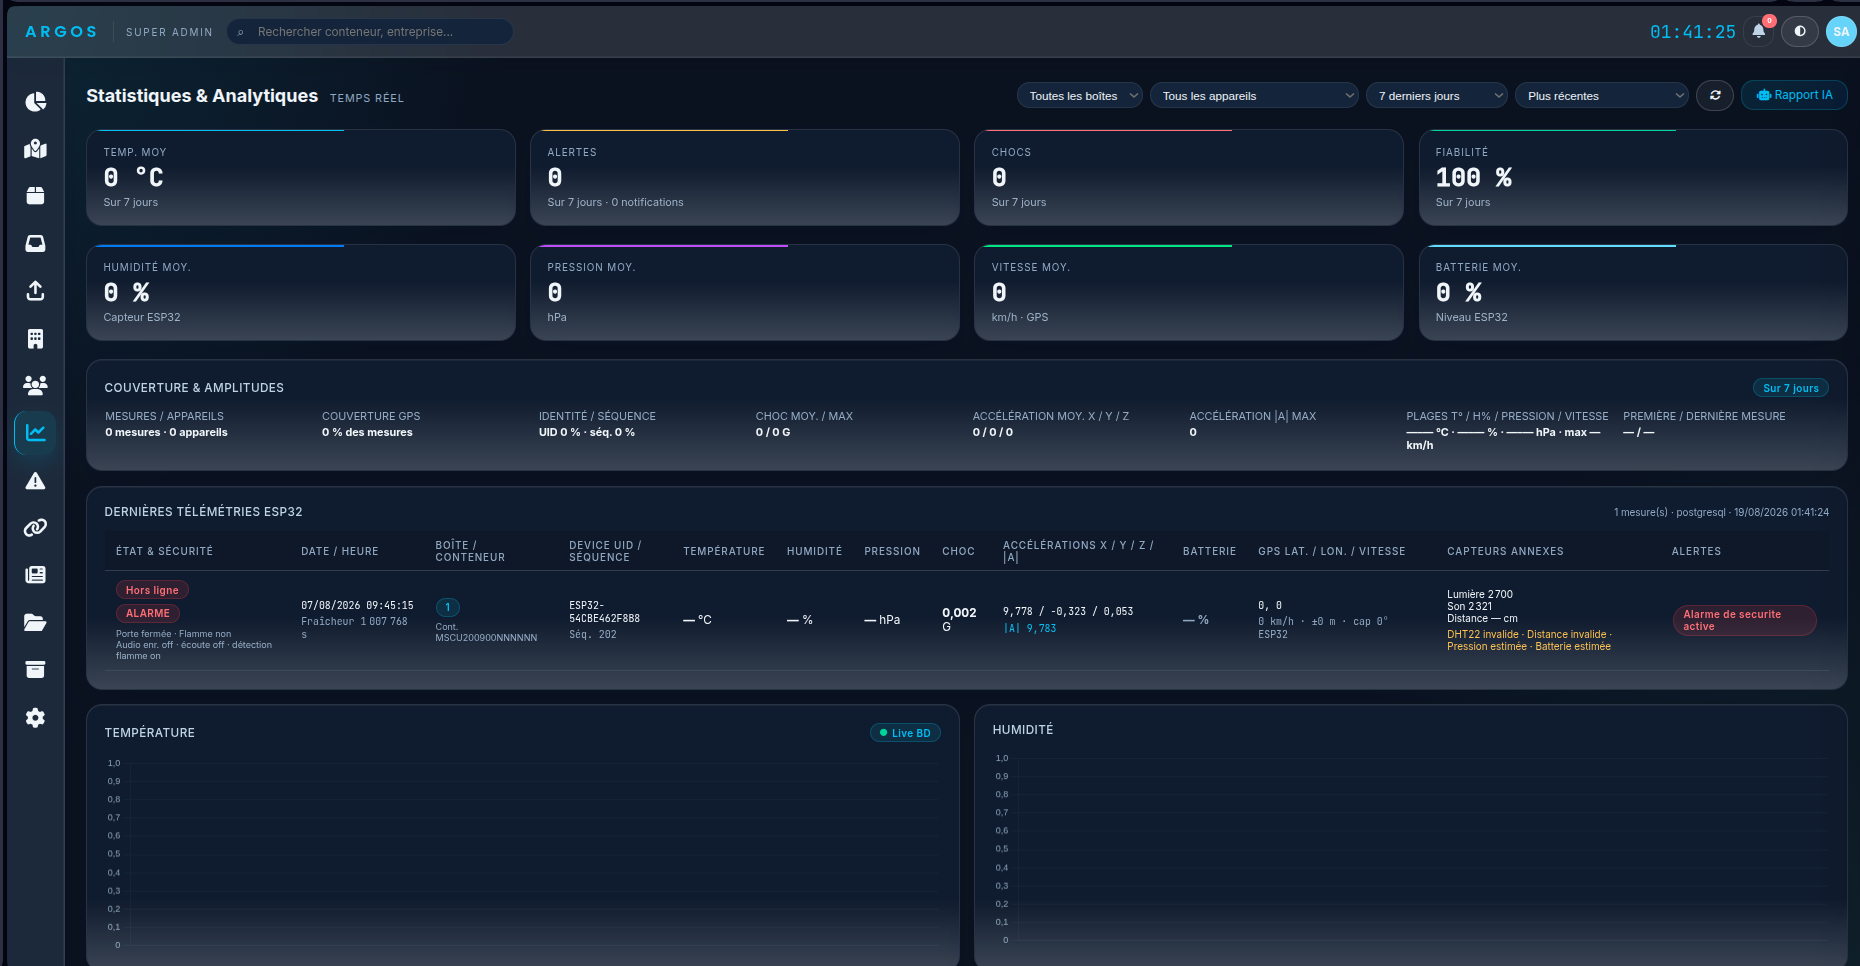
\includegraphics[width=0.66\textwidth]{figures/donnee.png}
\caption{Tableau de bord de supervision ARGOS}
\label{fig-dashboard-argos}
\end{figure}
\tablesourcepromoteurs


\subsection{Validation expérimentale}

\subsubsection{Tests déjà présents}

Les tests logiciels couvrent notamment la validation des coordonnées, les
types de capteurs, les statuts de commande, l'identité signée, le
provisionnement, la résolution QR et la protection des documents. Ils
constituent une validation du contrat logiciel entre le dispositif et le
backend.

\subsubsection{Protocole de mesures sur le prototype physique}

\begin{table}[!htbp]
\centering
\caption{Plan de validation expérimentale du prototype}
\label{tab-validation-prototype}
\begin{tabularx}{\textwidth}{@{}p{3.5cm} X p{3.2cm}@{}}
\tableheadrow \thc{Mesure} & \thc{Méthode proposée} & \thc{Résultat} \\
\midrule
Latence de télémétrie & Mesurer le délai entre l'émission série et la
confirmation du serveur sur 100 messages & Intervalle d'actualisation : 2~s \\
\hline
Taux de livraison & Comparer les séquences émises aux messages persistés,
avec et sans coupure réseau & 900 messages transmis sur 900 (100~\%) \\
\hline
Précision GPS & Comparer plusieurs positions à une référence connue en
extérieur & Précision horizontale : 5~m \\
\hline
Température, humidité et pression & Comparer les capteurs à des instruments de référence
dans plusieurs conditions & 25,45--28,55~\textdegree C ; 64,6--71,4~\% ;
1007,65--1010,35~hPa \\
\hline
Choc et vitesse & Étalonner le MPU-6050, provoquer des accélérations contrôlées
et comparer la vitesse fusionnée à la vitesse GNSS & Choc maximal : 7,35~g ;
vitesse : 54--70~km/h \\
\hline
Autonomie & Calculer puis vérifier la durée avec la batterie réellement
installée & Batterie : 100~\% à 98~\% après 30~min \\
\hline
Réaction à une alerte & Provoquer un dépassement contrôlé et mesurer le délai
jusqu'à la notification & Alerte déclenchée dès le dépassement de 5~g \\
\tablebottomrule
\end{tabularx}
\end{table}
\tablesourcepromoteurs

La réalisation du prototype démontre la continuité technique entre
l'acquisition embarquée, la communication réseau, la validation serveur, la
persistance et la supervision web. Le simulateur permet de tester les mêmes
contrats d'API indépendamment du montage physique. Le protocole expérimental
défini dans ce chapitre assure la traçabilité des performances mesurées lors
de la validation finale.
\\
\\
\\
\\
\\
\\
\\
\\
\\
\\
\\
\\
\\
\\
\\
\\
\subsection{Processus de déploiement}
\begin{figure}[h]
    \centering
    \begin{tikzpicture}[
        node distance=1.8cm,
        auto,
        % Style des boîtes d'étape
        box/.style={
            rectangle,
            rounded corners=4pt,
            draw=black, 
            thick,
            fill=blue!5,
            text width=11cm,
            align=left,
            inner sep=8pt,
            minimum height=1cm
        },
        % Style de la boîte finale
        finalbox/.style={
            rectangle,
            rounded corners=4pt,
            draw=green!60!black, 
            thick,
            fill=green!10,
            text width=11cm,
            align=center,
            inner sep=8pt,
            minimum height=1cm
        },
        % Style des flèches
        arrow/.style={
            thick,
            ->,
            >=stealth
        }
    ]

    % Définition des nœuds (étapes)
    \node[box] (step1) {\textbf{1. Financement \& Incubation} \\ Levée de fonds (prêts bancaires, investisseurs) et accompagnement par l'incubateur de SUP'PTIC.};
    
    \node[box, below of=step1, yshift=-0.5cm] (step2) {\textbf{2. Création \& Certification d'Entreprise} \\ Structuration juridique et certification officielle du projet sous l'entité ARGOS.};
    
    \node[box, below of=step2, yshift=-0.5cm] (step3) {\textbf{3. Agrément International (OMI)} \\ Négociations avec l'Organisation Maritime Internationale pour certifier la conformité, la fiabilité et la déployabilité de la solution.};
    
    \node[box, below of=step3, yshift=-0.5cm] (step4) {\textbf{4. Facilitation Douanière} \\ Enregistrement du dispositif à la douane en tant qu'« équipement de transit » afin de bénéficier d'exonérations fiscales.};
    
    \node[box, below of=step4, yshift=-0.5cm] (step5) {\textbf{5. Déploiement Commercial} \\ Présentation de la solution aux partenaires commerciaux, appuyée par une preuve de concept (PoC) garantissant la véracité des données.};
    
    \node[box, below of=step5, yshift=-0.5cm] (step6) {\textbf{6. Partenariats Assurances} \\ Négociations avec les compagnies d'assurance pour imposer l'installation du dispositif ARGOS sur les conteneurs couverts.};
    
    \node[finalbox, below of=step6, yshift=-0.5cm] (step7) {\textbf{7. Mise sur le Marché \& Opérationnalisation} \\ La solution ARGOS est officiellement déployée et fonctionnelle sur le marché de la logistique.};

    % Tracé des flèches
    \draw[arrow] (step1) -- (step2);
    \draw[arrow] (step2) -- (step3);
    \draw[arrow] (step3) -- (step4);
    \draw[arrow] (step4) -- (step5);
    \draw[arrow] (step5) -- (step6);
    \draw[arrow] (step6) -- (step7);

    \end{tikzpicture}
    \caption{Feuille de route du déploiement de la solution ARGOS}
    \label{fig:deploiement_argos}
\end{figure}
	
	% ============================================================
	% CONCLUSION GÉNÉRALE
	% ============================================================
	\chapter*{Conclusion générale}
\addcontentsline{toc}{chapter}{Conclusion générale}
\argossetpart{CONCLUSION GÉNÉRALE}
\argossetchapter{Conclusion générale}

Le transport maritime conteneurisé constitue l'une des composantes essentielles du commerce mondial\cite{unctad2025}. Pourtant, un conteneur sec, dépourvu d'alimentation et de connectivité embarquées, ne permet pas de suivre en continu l'intégrité physique de la marchandise durant le transit. Cette opacité, source de litiges et de pertes financières, se double d'une contrainte réglementaire renforcée par les amendements SOLAS/MARPOL de janvier 2026\cite{omi2026}, particulièrement sensible sur les corridors camerounais et centrafricains\cite{corridor_transit,logcluster}. C'est dans ce contexte que s'inscrit le projet ARGOS, boîte noire logistique connectée visant à assurer la continuité numérique et l'intégrité physique de la chaîne conteneurisée, de la mer jusqu'à la destination finale.

Ce mémoire a conduit une démarche en trois volets. L'étude de marché a validé la pertinence commerciale du projet en substituant à la vente de matériel un modèle de service indexé sur la valeur de la marchandise (3\,\%), levant la barrière à l'entrée pour les transporteurs et instaurant une relation tripartite entre client finaux, propriétaires de conteneurs et promoteurs d'ARGOS. L'étude de faisabilité financière a confirmé la robustesse économique du projet, avec une VAN positive (Tableau~\ref{tab:van}), un TRI de 89,5\,\% et un délai de récupération d'environ vingt mois (Tableau~\ref{tab:tri_drci}). Enfin, l'étude technique et la réalisation du prototype ont démontré la faisabilité opérationnelle : architecture logicielle complète, base de données de 48 tables et 559 champs, chaîne d'acquisition embarquée (température, humidité, choc, position GPS, audio) reliée à une plateforme web de supervision, évaluée par les essais du Tableau~\ref{tab-validation-prototype}.

L'apport principal de ce travail réside dans le caractère intégré de la solution : ARGOS associe traçabilité, intégrité physique, preuve numérique horodatée et modèle économique adapté aux réalités d'Afrique centrale, où l'autonomie énergétique et la couverture réseau intermittente sont des contraintes majeures. Le projet répond ainsi aux trois objectifs fixés en introduction : sécurisation du conteneur en temps réel, réduction des pertes liées aux litiges et prise en compte des instruments internationaux pertinents, notamment SOLAS et le code IMDG\cite{imo_solas,imo_imdg}.

Ce travail comporte des limites assumées, qui tracent les développements futurs. L'intégration matérielle et les essais réels des modems LTE-M/NB-IoT et LoRaWAN restent à mener au-delà de la simulation ; la transmission dépend aujourd'hui des réseaux cellulaires terrestres, d'où des zones d'ombre qu'un module hybride cellulaire-satellitaire viendrait combler. L'infrastructure logicielle repose sur des services d'hébergement tiers ; pour garantir la souveraineté numérique des données du fret, un serveur physique local dédié devrait être déployé. Le service d'enrichissement BIC écrit encore des noms de colonnes obsolètes (\textit{type\_code}, \textit{tare\_mass\_kg}, \textit{max\_gross\_mass\_kg}) alors que le schéma actif expose \textit{iso\_type\_code}, \textit{tare\_kg} et \textit{max\_gross\_kg} ; ce contrat de données doit être aligné avant de considérer l'enrichissement comme fiable. L'interface, limitée au français et à l'anglais, gagnerait à être internationalisée pour les équipages et opérateurs portuaires transfrontaliers. Bien que les données générées soient scellées et auditables, leur force probante auprès des assurances et autorités suppose encore audits et certifications ; l'OMI établit les conventions maritimes mais ne certifie pas directement un boîtier commercial\cite{imo_solas,imo_imdg}. Enfin, les fonctionnalités décisionnelles reposant sur des algorithmes génériques, des travaux visant à entraîner un modèle d'IA dédié aux réalités du secteur portuaire.

En définitive, le projet ARGOS démontre qu'une solution de traçabilité active, techniquement maîtrisée et économiquement viable, peut transformer le conteneur passif en un objet connecté et digne de confiance. Les prochaines étapes telque la validation en conditions réelles, l'homologations et la spécialisation d'un modèle d'IA dédié ouvrent la voie à un déploiement à plus grande échelle sur les corridors logistiques d'Afrique centrale, et à une contribution africaine aux enjeux mondiaux de sécurisation du fret maritime.


    \pagenumbering{roman}
	\setcounter{page}{1}
	
	% ============================================================
	% RÉFÉRENCES
	% ============================================================
	\chapter*{RÉFÉRENCES}
\addcontentsline{toc}{chapter}{RÉFÉRENCES}
\markboth{\sffamily\small\textsc{RÉFÉRENCES}}{}

\begin{thebibliography}{99}

\argosbibitem{unctad2025}
\argosbibitem{cts2025}
\argosbibitem{gmi2025}
\argosbibitem{omi2026}
\argosbibitem{pad2025}
\argosbibitem{corridor2025}
\argosbibitem{pak2026}
\argosbibitem{banquemondiale2025}
\argosbibitem{tresor2025}
\argosbibitem{cemac2025}
\argosbibitem{cncc2025}
\argosbibitem{agenceecofin}
\argosbibitem{esp32}
\argosbibitem{sim7000}
\argosbibitem{ublox}
\argosbibitem{iso21502}
\argosbibitem{cncc_missions}
\argosbibitem{apn_missions}
\argosbibitem{loi2010_tel}
\argosbibitem{iso2018}
\argosbibitem{art}
\argosbibitem{imo_web}
\argosbibitem{wsc2025}
\argosbibitem{logcluster}
\argosbibitem{loi2010_cyber}
\argosbibitem{imo_solas}
\argosbibitem{imo_imdg}
\argosbibitem{rgpd_officiel}
\argosbibitem{art_homologation}
\argosbibitem{ohada_auscgie}
\argosbibitem{cgi_cameroun}
\argosbibitem{incitations2025}
\argosbibitem{cnps_employeurs}
\argosbibitem{loi2024_donnees}
\argosbibitem{minpmeesa_cfce}
\argosbibitem{bpifrance}
\argosbibitem{vernimmen_dalloz}
\argosbibitem{vernimmen_fnac}
\argosbibitem{flask}
\argosbibitem{postgresql}
\argosbibitem{leaflet}
\argosbibitem{chartjs}
\argosbibitem{corridor_transit}
\argosbibitem{supptic2024}
\argosbibitem{playwright}
\argosbibitem{tailwind}
\argosbibitem{lcsc}
\argosbibitem{mermaid}
\argosbibitem{antic}
\argosbibitem{babu_mbuangi2023}

\end{thebibliography}


	\clearpage
\phantomsection
\addcontentsline{toc}{chapter}{Index}
\chapter*{Index}
\markboth{INDEX}{INDEX}

Le présent index répertorie les annexes et illustrations documentaires clés de la solution ARGOS, facilitant leur repérage au sein du rapport.

\begin{itemize}
    \item textbf{Formulaire d'enquête} \dotfill \pageref{tab:synthese-enquete}

    \clearpage
    \phantomsection
    \addcontentsline{toc}{section}{Formulaire d'enquête détaillé}

    % Insère toutes les pages du fichier cc.pdf à partir de la page 1 jusqu'à la fin
    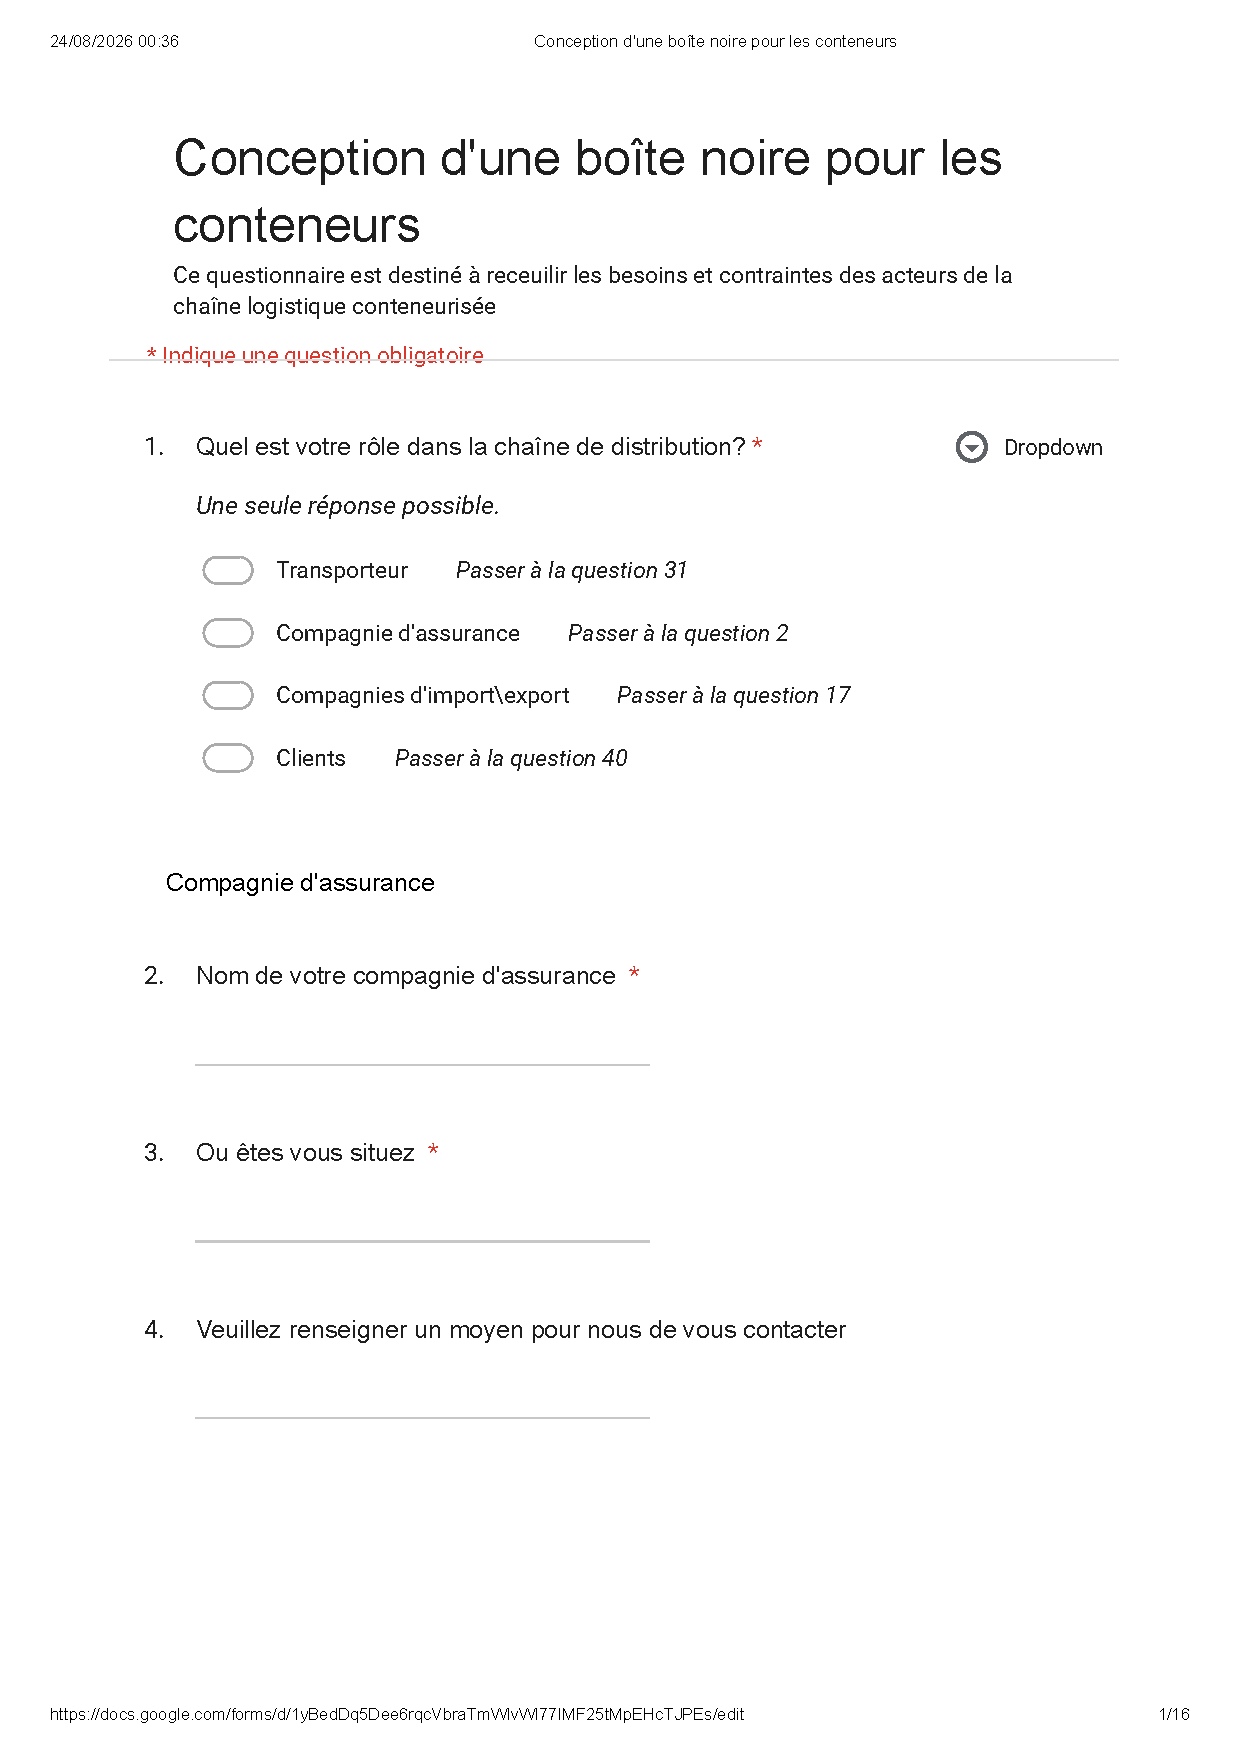
\includepdf[pages=-, scale=0.85, width=\textwidth, keepaspectratio=true]{figures/cc.pdf}

    \item \textbf{Logo ARGOS} \dotfill \pageref{fig-argos-chaine-valeur}

    \begin{figure}[htbp]
    \centering
    
\includegraphics[width=0.66\textwidth]{figures/logo.jpeg}
    \caption{Tableau de bord de supervision ARGOS}
    \label{fig-index-logo-argos}
    \end{figure}

\end{itemize}

	
	% ============================================================
	% TABLE DES MATIÈRES DÉTAILLÉE (fin du document)
	% ============================================================
	\cleardoublepage
	\tableofcontents
	\thispagestyle{plain}
	
\end{document}
